% !TeX root = ./thesis.tex
% export PATH=/usr/local/texlive/2021/bin/x86_64-linux:$PATH
\documentclass[twoside,openright,titlepage,numbers=noenddot,headinclude,footinclude=true,cleardoublepage=empty,BCOR=5mm,fontsize=10pt,dutch,english]{scrbook}
                     
\newlength{\mytextwidth}
\setlength{\mytextwidth}{288pt}

\newlength{\mytextheight}
\setlength{\mytextheight}{555pt}

\setlength{\footskip}{25pt}

\usepackage[papersize={17cm,24cm}, width=\mytextwidth, height=\mytextheight,hmarginratio={1:2},vmarginratio={1:1},bindingoffset=4mm]{geometry}

\PassOptionsToPackage{eulerchapternumbers,listings, pdfspacing, subfig,beramono,thesispaper}{classicthesis}					

\usepackage{ifthen}
\newboolean{enable-backrefs}
\setboolean{enable-backrefs}{false}

% Personal data
\newcommand{\myTitle}{Unsupervised Brain Anomaly Detection in MR Images\xspace}
\newcommand{\mySubtitle}{}
\newcommand{\myName}{Samuel Botter Martins\xspace}
\newcommand{\myUni}{University of Groningen\xspace}

% Setup and useful commands
\newcounter{dummy} 
\newlength{\abcd} 
\providecommand{\mLyX}{L\kern-.1667em\lower.25em\hbox{Y}\kern-.125emX\@}
\newcommand{\abbr}[1]{\textsc{\MakeLowercase{#1}}}

\newlength{\figureHalf}\setlength{\figureHalf}{139.74pt}
\newlength{\figureThird}\setlength{\figureThird}{90.32pt}
\newlength{\figureFourth}\setlength{\figureFourth}{65.61pt}

\newlength{\figureHalfBigSkip}\setlength{\figureHalfBigSkip}{129.8pt}
\newlength{\figureThirdBigSkip}\setlength{\figureThirdBigSkip}{77.0667pt}
\newlength{\figureFourthBigSkip}\setlength{\figureFourthBigSkip}{50.7pt}

% More packages
\usepackage{verbatim}
\usepackage{printlen}
\usepackage{makeidx}

\usepackage[lining]{libertine}
\usepackage[T1]{fontenc}
\usepackage{textcomp}
\usepackage[fleqn]{amsmath}
\usepackage{amsthm}
\usepackage[libertine]{newtxmath}
\usepackage{mathtools}
\usepackage[bb=pazo,bbscaled=0.94,cal=cm,calscaled=0.96]{mathalfa}
\usepackage{bm}
\usepackage{rotating}
\usepackage{mdframed}			% Create frames

% \usepackage[ruled,noline,noend]{algorithm2e}
% \usepackage[ruled,vlined,linesnumbered]{algorithm2e}
% \usepackage{algorithm}
\usepackage{algorithmic}

\renewcommand{\algorithmicrequire}{\textbf{Input:}}
\renewcommand{\algorithmicensure}{\textbf{Output:}}

\usepackage{sidecap}
\usepackage{marginnote}
\usepackage{tikz}
\usetikzlibrary{arrows,calc,positioning}
\usepackage{tabulary}

\usepackage{enumitem}

\newenvironment{myabstract}%
{\textsc{abstract:} \slshape\footnotesize }%
{}

\PassOptionsToPackage{utf8}{inputenc}	
 \usepackage{inputenc}				

\PassOptionsToPackage{dutch,english,portuguese}{babel}
 \usepackage{babel}					

\PassOptionsToPackage{square,numbers,sort&compress}{natbib}
% \PassOptionsToPackage{round}{natbib}
\usepackage{natbib}				

\usepackage{scrhack} % fix warnings when using KOMA with listings package          
\usepackage{xspace} % to get the spacing after macros right  
\usepackage{mparhack} % get marginpar right
\PassOptionsToPackage{printonlyused,smaller}{acronym}
	\usepackage{acronym} 
\ifdefined\bflabel
	\renewcommand{\bflabel}[1]{{#1}\hfill} % fix the list of acronyms
\else
\fi


% Setup floats: tables, (sub)figures, and captions
\usepackage{tabularx} % better tables
	\setlength{\extrarowheight}{3pt} % increase table row height
\newcommand{\tableheadline}[1]{\multicolumn{1}{c}{\spacedlowsmallcaps{#1}}}
\newcommand{\myfloatalign}{\centering} % to be used with each float for alignment
\usepackage{caption}
\captionsetup{format=hang,font=small}
\usepackage{subfig}  

%Setup code listings
\usepackage{listings} 
\lstset{language=[LaTeX]Tex,%C++,
    keywordstyle=\color{RoyalBlue},%\bfseries,
    basicstyle=\small\ttfamily,
    %identifierstyle=\color{NavyBlue},
    commentstyle=\color{Green}\ttfamily,
    stringstyle=\rmfamily,
    numbers=none,%left,%
    numberstyle=\scriptsize,%\tiny
    stepnumber=5,
    numbersep=8pt,
    showstringspaces=false,
    breaklines=true,
    frameround=ftff,
    frame=single,
    belowcaptionskip=.75\baselineskip
    %frame=L
} 

% PDFLaTeX, hyperreferences and citation backreferences
\PassOptionsToPackage{pdftex,hyperfootnotes=false,pdfpagelabels,breaklinks}{hyperref}
	\usepackage{hyperref}
\pdfcompresslevel=9
\pdfadjustspacing=1 
\PassOptionsToPackage{pdftex}{graphicx}
	\usepackage{graphicx} 
\usepackage[capitalise]{cleveref}

% Setup the style of the backrefs from the bibliography
\newcommand{\backrefnotcitedstring}{\relax}%(Not cited.)
\newcommand{\backrefcitedsinglestring}[1]{(Cited on page~#1.)}
\newcommand{\backrefcitedmultistring}[1]{(Cited on pages~#1.)}
\ifthenelse{\boolean{enable-backrefs}}%
{%
		\PassOptionsToPackage{hyperpageref}{backref}
		\usepackage{backref} % to be loaded after hyperref package 
		   \renewcommand{\backreftwosep}{ and~} % separate 2 pages
		   \renewcommand{\backreflastsep}{, and~} % separate last of longer list
		   \renewcommand*{\backref}[1]{}  % disable standard
		   \renewcommand*{\backrefalt}[4]{% detailed backref
		      \ifcase #1 %
		         \backrefnotcitedstring%
		      \or%
		         \backrefcitedsinglestring{#2}%
		      \else%
		         \backrefcitedmultistring{#2}%
		      \fi}%
}{\relax}    

% Hyperreferences
\hypersetup{%
    colorlinks=true, linktocpage=true, pdfstartpage=3, pdfstartview=FitV,%
    breaklinks=true, pdfpagemode=UseNone, pageanchor=true, pdfpagemode=UseOutlines,%
    plainpages=false, bookmarksnumbered, bookmarksopen=true, bookmarksopenlevel=1,%
    hypertexnames=true, pdfhighlight=/O,
    urlcolor=black, linkcolor=black, citecolor=black, 
    pdftitle={\myTitle},%
    pdfauthor={\textcopyright\ \myName},%
    pdfsubject={},%
    pdfkeywords={},%
    pdfcreator={pdfLaTeX},%
    pdfproducer={LaTeX with hyperref and classicthesis}%
}   

% Setup autoreferences
\makeatletter
\@ifpackageloaded{babel}%
    {%
       \addto\extrasenglish{%
					\renewcommand*{\figureautorefname}{Figure}%
					\renewcommand*{\tableautorefname}{Table}%
					\renewcommand*{\partautorefname}{Part}%
					\renewcommand*{\chapterautorefname}{Chapter}%
					\renewcommand*{\sectionautorefname}{Section}%
					\renewcommand*{\subsectionautorefname}{Section}%
					\renewcommand*{\subsubsectionautorefname}{Section}% 	
				}%
       \addto\extrasngerman{% 
					\renewcommand*{\paragraphautorefname}{Absatz}%
					\renewcommand*{\subparagraphautorefname}{Unterabsatz}%
					\renewcommand*{\footnoteautorefname}{Fu\"snote}%
					\renewcommand*{\FancyVerbLineautorefname}{Zeile}%
					\renewcommand*{\theoremautorefname}{Theorem}%
					\renewcommand*{\appendixautorefname}{Anhang}%
					\renewcommand*{\equationautorefname}{Gleichung}%        
					\renewcommand*{\itemautorefname}{Punkt}%
				}%	
			\providecommand{\subfigureautorefname}{\figureautorefname}%  			
    }{\relax}
\makeatother


\listfiles

\usepackage{classicthesis} 

% Further adjustments (experimental)
\usepackage{bibentry}
\nobibliography*

\providecommand{\doi}[1]{\abbr{DOI} \href{http://dx.doi.org/#1}{\urlstyle{same}\nolinkurl{#1}}}

\emergencystretch=1em

\newtheoremstyle{theoremStyle}
    {\topsep}                    % Space above
    {\topsep}                    % Space below
    {\itshape}                   % Body font
    {}                           % Indent amount
    {\scshape}                   % Theorem head font
    {.}                          % Punctuation after theorem head
    {.5em}                       % Space after theorem head
    {}  % Theorem head spec (can be left empty, meaning ‘normal’)
\theoremstyle{theoremStyle}
\newtheorem{theorem}{Theorem}
\newtheorem{lemma}[theorem]{Lemma}
\newtheorem{corollary}[theorem]{Corollary}
\newtheorem{proposition}[theorem]{Proposition}

\newtheoremstyle{exampleStyle}
    {0}                          % Space above
    {0}                          % Space below
    {}                           % Body font
    {}                           % Indent amount
    {\scshape}                   % Theorem head font
    {.}                          % Punctuation after theorem head
    {.5em}                       % Space after theorem head
    {}  % Theorem head spec (can be left empty, meaning ‘normal’)
\theoremstyle{exampleStyle}
\newtheorem{example}[theorem]{Example}
\usepackage{mdframed}
\surroundwithmdframed[bottomline=false,topline=false,rightline=false,
	linewidth=1pt,
	linecolor=gray,
	%innerleftmargin=7pt,
	skipabove=\topsep,
	skipbelow=0,
	innertopmargin=0,
	innerbottommargin=0]{example}

% Counters
\numberwithin{equation}{chapter}
\numberwithin{theorem}{chapter}
\numberwithin{figure}{chapter}

% CRef names
\crefname{algocf}{Alg.}{Algs.}
\Crefname{algocf}{Algorithm}{Algorithms}

\setlength{\marginparwidth}{8em}%

% Personal commands
\newcommand{\makenote}[1]{{ \color{red} [#1]}}

\DeclareMathOperator*{\argmax}{arg\,max}
\newcommand{\defaultwidth}{width=}

\DeclareMathOperator{\cov}{cov}
\DeclareMathOperator{\corr}{corr}
\DeclareMathOperator{\std}{std}
\DeclareMathOperator{\var}{var}
\DeclareMathOperator{\Val}{Val}

\DeclareMathOperator*{\KL}{KL}
\newcommand{\bs}{\bm}

\newcommand\independent{\protect\mathpalette{\protect\independenT}{\perp}}
\def\independenT#1#2{\mathrel{\rlap{$#1#2$}\mkern2mu{#1#2}}}

%% -----------------------------------------------
% My own commands
%% -----------------------------------------------

\newcommand{\fold}[1]{\mathcal{#1}}
\newcommand{\set}[1]{\mathbb{#1}}
\newcommand{\vecx}[1]{\boldsymbol{#1}}
\newcommand{\state}{\vecx{\phi}}

\newcommand{\chref}[1]{\autoref{ch:#1}}
\newcommand{\secref}[1]{\autoref{sec:#1}}
\newcommand{\figref}[1]{\autoref{fig:#1}}
\newcommand{\eqnref}[1]{\autoref{eqn:#1}}
\newcommand{\tabref}[1]{\autoref{tab:#1}}
\newcommand{\quadref}[1]{\autoref{quad:#1}}
\newcommand{\parref}[1]{\autoref{par:#1}}	
\newcommand{\coderef}[1]{\autoref{code:#1}}	
\newcommand{\appref}[1]{\autoref{app:#1}}
\newcommand{\itemref}[1]{\autoref{item:#1}}

\hypersetup{
	pdftitle={\myTitle}, 
	pdfauthor={\myName},
	pdfsubject={},
	pdfcreator={},
	pdfkeywords={}, 
	colorlinks=true,       		% false: boxed links; true: colored links
	linkcolor=blue,          	% color of internal links
	citecolor=blue,        		% color of links to bibliography
	filecolor=magenta,      	% color of file links
	urlcolor=blue,
	bookmarksdepth=4,
	plainpages = false,
  	linktocpage
}

% Just right frame
\newmdenv[leftline=false, topline=false, bottomline=false]{rightframe}

% Left and bottom frame
\newmdenv[topline=false, rightline=false]{leftbot}

% Top and bottom frame
\newmdenv[rightline=false, leftline=false]{topbot}

\newcommand{\hyp}[1]{
	\begin{topbot}
		\vspace{.5cm}	
		% \setlength{\parindent}{4em}
		% \setlength{\parskip}{2em}
		\noindent
		\emph{Hyphotesis: ``{#1}''}.
		\vspace{.5cm}
	\end{topbot}
}


%%%%%%% SAMUEL'S DEFINITIONS %%%%%%%%
\usepackage[ruled,vlined,linesnumbered]{algorithm2e}
\newcommand{\la}{\leftarrow}

\usepackage[]{appendix}
\usepackage{colortbl}
\usepackage{booktabs} 
\usepackage{hyperref}
\usepackage{multirow}
\usepackage{rotating}
\usepackage{subfig}
\usepackage{xprintlen}
% \printlen[2][cm]{\columnwidth} % to find out the column width in cm

% customizing colors from url, citations, and links
% RoyalBlue defined by the command \definecolor in classicthesis.sty
\hypersetup{%
	urlcolor=RoyalBlue,
	citecolor=RoyalBlue,
	linkcolor=RoyalBlue
}


% footnotes without numbers
\newcommand\blfootnote[1]{%
	\begingroup
	\renewcommand\thefootnote{}\footnote{#1}%
	\addtocounter{footnote}{-1}%
	\endgroup
}


\newcommand{\etal}{\emph{et al.}}
\newcommand{\eg}{\emph{e.g., }}
\newcommand{\ie}{\emph{i.e., }}

\newcommand{\fig}{Fig.}
\newcommand{\figs}{Figs.}

\newcommand{\tbf}[1]{\textbf{#1}}
\newcommand{\tit}[1]{\textit{#1}}
\newcommand{\mbf}[1]{\mathbf{#1}}

% review highlighting
\newcommand{\red}[1]{\textcolor{red}{#1}}
\newcommand{\blue}[1]{\textcolor{blue}{#1}}
\newcommand{\alex}[1]{\textcolor{red}{\textbf{Alex:} #1}}
\newcommand{\falcao}[1]{\textcolor{orange}{\textbf{Falcao:} #1}}
\newcommand{\samuel}[1]{\textcolor{magenta}{\textbf{Samuel:} #1}}


\newcommand{\adapro}{AdaPro\xspace}
\newcommand{\sosms}{SOSM-S\xspace}
\newcommand{\volbrain}{volBrain\xspace}
\newcommand{\malf}{MALF\xspace}

% \interfootnotelinepenalty=10000



%% Eduardo's additions
\usepackage[utf8]{inputenc}
\DeclareUnicodeCharacter{2010}{-}% support older LaTeX versions
\usepackage{rotating}
\usepackage[font=itshape]{quoting}
\newcommand{\eduardo}[1]{\textcolor{red}{#1}}
\newcommand{\alex}[1]{\textcolor{blue}{#1}}
\newcommand{\joao}[1]{\textcolor{blue}{#1}}
%% Be careful here


\hyphenation{net-works}

\begin{document}

\sloppy

\frenchspacing
\raggedbottom
\selectlanguage{english}

\pagenumbering{roman}
\pagestyle{plain}

% Front matter
\begin{titlepage}
	\begin{addmargin}[-1cm]{-3cm}
    \begin{center}
        \large  

        \hfill

        \vfill

        \begingroup
            \color{Maroon}\spacedallcaps{\myTitle} \\ \bigskip
        \endgroup

        \spacedlowsmallcaps{\myName}

        \vfill

        \mySubtitle \\ \medskip   

        \vfill                      

    \end{center}  
  \end{addmargin}       
\end{titlepage}   
\thispagestyle{empty}

\hyphenation{}

\null
\vfill

\noindent Cover: add cover image description.
\vspace{1.5cm}

\noindent\myTitle\\
\hangindent=1em

\noindent \myName\\
PhD Thesis\\

\vspace{1.5cm}
\noindent This thesis is the result of a joint PhD between the Federal University of Rio Grande do Sul and the University of Groningen. \\

\vspace{1.5cm}

% TODO: ISBN when there is one
%\noindent \abbr{ISBN} 978-90-367-9288-2 (printed version)\\
%\abbr{ISBN} 978-90-367-9287-5 (electronic version)


\thispagestyle{empty}

\begin{addmargin}[-1cm]{-3cm}

\includegraphics[width=7.38cm]{figures/rugr_logoen_zwart_cmyk}

\begin{center}

\large 

\vfill\vfill\vfill\vfill\vfill

{\LARGE\textbf{\myTitle}}

\vfill\vfill\vfill\vfill\vfill

{\Large\textbf{PhD thesis}}

\vfill\vfill\vfill\vfill

to obtain the degree of PhD at the\\
University of Groningen\\
on the authority of the\\
Rector Magnificus Prof.\ C. Wijmenga\\
and in accordance with\\
the decision by the College of Deans,
and\\
to obtain the degree of PhD at the\\
University of Rio Grande do Sul\\
on the authority of\\
Rector Magnificus Prof.\ C. Bulhões Mendes.\\
\vfill
Double PhD Degree\\
\vfill

This thesis will be defended in public on\\

\vfill
% TODO: fill this when after room is reserved
Weekday DD Month YYYY at HH.MM hours\\

\vfill\vfill\vfill\vfill

by

\vfill\vfill\vfill\vfill

{\Large\textbf{\myName}}\\

\vfill
born on March 30th, 1995\\
in Porto Alegre, Brazil 
\end{center}
\end{addmargin}

\newpage
\thispagestyle{empty}
{\large
\noindent\textbf{Supervisors}\\
Prof. dr. Alexandru Cristian Telea\\
Prof. dr. João Luiz Dihl Comba\\

\noindent\textbf{Assessment committee}\\
Prof. Assessment prof1\\
Prof. Assessment prof2\\
Prof. Assessment prof3\\
Prof. Assessment prof4\\

\vfill
}


\pagestyle{scrheadings}

\cleardoublepage\null
\vfill

\hfill \begin{minipage}{.75\textwidth}
Just about anything looks better from a distance.

\hfill --- Haruki Murakami 
\end{minipage}

\cleardoublepage

\cleardoublepage\begingroup

\let\clearpage\relax
\let\cleardoublepage\relax
\let\cleardoublepage\relax

\manualmark
\markboth{\spacedlowsmallcaps{Abstract}}{\spacedlowsmallcaps{Abstract}} 
\phantomsection 

\pdfbookmark[0]{Abstract}{Abstract}
\chapter*{Abstract}

When it comes to tools and techniques designed to help understanding complex abstract data, visualization methods play a prominent role. They enable human operators to leverage their pattern finding, outlier detection, and questioning abilities to visually reason about a given dataset. Many methods exist that create suitable and useful visual representations of \emph{static} abstract, non-spatial, data. However, for \emph{temporal} abstract, non-spatial, datasets, in which the data changes and evolves through time, far fewer visualization techniques exist.

This thesis focuses on the particular cases of temporal hierarchical data representation via dynamic treemaps, and temporal high-dimensional data visualization via dynamic projections. We tackle the joint question of how to extend projections and treemaps to stably, accurately, and scalably handle temporal multivariate and hierarchical data. In both cases, the literature for the static techniques is rich and the state-of-the-art methods have proven to be valuable tools in data analysis. Their temporal/dynamic counterparts, however, are not as well studied, and, until recently, there were few hierarchical and high-dimensional methods that explicitly took into consideration the temporal aspect of the data. In addition, there are few or no metrics to assess the quality of these temporal mappings, and even fewer comprehensive benchmarks to compare these methods. 

This thesis addresses the abovementioned shortcomings. For both dynamic treemaps and dynamic projections. We propose ways to accurately measure temporal stability; we evaluate existing methods considering the tradeoff between stability and visual quality; and we propose new methods that strike a better balance between stability and visual quality than existing state-of-the-art techniques. We demonstrate our methods with a wide range of real-world data, including an application of our new dynamic projection methods to support the analysis and classification of hyperkinetic movement disorder data.

\newpage

\selectlanguage{dutch}

\manualmark
\markboth{\spacedlowsmallcaps{Samenvatting}}{\spacedlowsmallcaps{Samenvatting}} 
\phantomsection 

\pdfbookmark[0]{Samenvatting}{samenvatting}
\chapter*{Samenvatting}

Thesis abstract in Dutch.

\newpage

\selectlanguage{portuguese}

\manualmark
\markboth{\spacedlowsmallcaps{Resumo}}{\spacedlowsmallcaps{Resumo}} 
\phantomsection 

\pdfbookmark[0]{Resumo}{resumo}
\chapter*{Resumo}

Thesis abstract in Portuguese.

\selectlanguage{english}

\endgroup			

\cleardoublepage\begingroup
\let\clearpage\relax
\let\cleardoublepage\relax
\let\cleardoublepage\relax

\manualmark
\markboth{\spacedlowsmallcaps{Publications}}{\spacedlowsmallcaps{Publications}} 
\phantomsection 

\pdfbookmark[0]{Publications}{publications}
\chapter*{Publications}
This thesis is the result of the following publications:
\begin{itemize}
\item Quantitative Comparison of Treemap Techniques for Time-Dependent Hierarchies (poster) ~\citep{vernier17} \footnote{Best Poster Award at Eurovis 2017}
\item Quantitative Comparison of Dynamic Treemaps for Software Evolution Visualization~\citep{vernier18software} \footnote{Distinguished paper award at VISSOFT 2018}
\item A Stable Greedy Insertion Treemap Algorithm for Software Evolution Visualization~\citep{vernier18git}
\item Selecting and Sharing Multidimensional Projection Algorithms~\citep{EspadotoSharing}
\item Quantitative Comparison of Time-Dependent Treemaps~\citep{vernier_treemap}
\item Quantitative Evaluation of Time-Dependent Multidimensional Projection Techniques~\citep{Vernier2020}
\item Guided Stable Dynamic Projections~\citep{Vernier2021}
\end{itemize}


\endgroup

\cleardoublepage\refstepcounter{dummy}
\pdfbookmark[0]{\contentsname}{tableofcontents}

\setcounter{tocdepth}{4} 
\setcounter{secnumdepth}{4}

\manualmark
\markboth{\spacedlowsmallcaps{\contentsname}}{\spacedlowsmallcaps{\contentsname}}

\tableofcontents 

\automark[section]{chapter}
\renewcommand{\chaptermark}[1]{\markboth{\spacedlowsmallcaps{#1}}{\spacedlowsmallcaps{#1}}}
\renewcommand{\sectionmark}[1]{\markright{\thesection\enspace\spacedlowsmallcaps{#1}}}



% Main matter
\cleardoublepage
\pagenumbering{arabic}

\chapter{Introduction}
\label{ch:intro}
%
As science and technology evolves, a myriad of data collections are produced. The common denominator of all these data collections is the same -- they are regarded as containing useful and usable information from which actionable evidence can be extracted, the latter leading to improvements in many directions -- increased sales, better customer support, more accurate assessments of phenomena, or, at a higher level, the advance of understanding of these phenomena that have created the data, and, thereby, an increase of knowledge and advancement to science. These datasets challenge their consumers in many ways. Several relevant aspects that induce such challenges include the \emph{size} of datasets (the `big data' revolution has made the efficient processing of terrabyte dataset collections a mandatory requirement for most application areas); the \emph{quality} of data (principled statistical analysis and modeling of phenomena captured by data require accurately measured and collected datasets); and the \emph{provenance} of data (one needs to know how the entire end-to-end pipeline of obtaining a given dataset looks like before being able to make strong statements concerning insights derived from the respective data).

Yet, the challenges of understanding data are not limited to the above issues. A separate, and equally important, one regards the \emph{structure} of data itself. By structure, we mean here the relations that connect the measured data samples, also called observations or data points, so as to allow scientists to infer high-level considerations about the underlying phenomena. Data structure regards many aspects, including, but not limited to, the \emph{nature} of the data samples (\emph{e.g.}, these can be quantitative, categorical, text, relational, or multimedia types); the \emph{dimensionality} of the samples (how many independent attributes are measured to yield a single data sample); the \emph{temporality} of data (are the samples part of a single measurement of a phenomenon done at a single moment in time, or are they spread over a time range); and the \emph{organization} of the samples (do the samples create a flat, unstructured, set, or are they organized in a more refined manner, to denote a part-whole relationship).

Among many methods for data analysis, including statistics and machine learning, \emph{visualization} has a special place. Data visualization essentially leverages the skills of the human operator in \emph{e.g.} pattern finding, outlier detection, and at a higher level discovering unknown relationships between the data samples and thereby the ability to pose valuable questions by depicting the measured data via visual representations. Further on, data visualization can be enhanced by \emph{visual analytics}, which leverages the interactive dimension to allow human operators to view data from various angles, pose questions, and most importantly, formulate, check, and (in)validate hypotheses that ultimately lead to understanding the phenomena that have generated the data in the first place.

Data visualization -- and by extension, visual analytics -- can be roughly split into two main subfields. \emph{Scientific visualization} is traditionally concerned with the visual exploration of datasets consisting of samples having a relatively low number of dimensions (measurements). More importantly, these data points sample \emph{continuous} phenomena that cover the evolution of natural systems in the 2D or 3D space that describes our physical world, \emph{e.g.}, the flow of fluids, evolution of weather systems, the observable Universe, or chemical, anatomical, or medical phenomena embedded in their respective sciences. While far from having solved all problems in these fields, scientific visualization can exploit the 2D or 3D embedding of the measured samples, and, more importantly, exploit the continuous nature of the sampled phenomena, by using well-understood sampling, aggregation, statistical, and signal reconstruction methodology.

\emph{Information visualization} aims at leveraging the visual exploration power for all datasets which do not fall within the scientific visualization realm, meaning datasets where samples (a) do not reside in physical 2D or 3D space and/or (b) where the sampled dimensions are not necessarily continuous. An enormous realm of datasets, arguably larger than the scientific visualization ones, falls into this class. Examples include arbitrary data tables in any database or graphs and networks. Major challenges of information visualization stem precisely from the \emph{abstract} nature of the data it needs to depict: Since this data does not (usually) have a physical counterpart, it is (a) far less clear than for the scientific visualization case how to \emph{map} this data to suitable visual representations. On the other hand, by their very definitions, visualizations are perceived as continuous phenomena by users looking at them -- whether this regards the \emph{spatial} distribution of visual shapes drawn or the \emph{temporal} dynamics of how visualizations change over time as the depicted data changes. Since abstract data does not have an inherent continuity, the fundamental question arises on how to map non-continuous data to continuous visual representations for a good interpretation. Additional issues concerning big data, such as aggregation and sampling, only complicate the picture.

In this thesis, we attack a part of the above problem by focusing on abstract data that has three specific aspects:

\begin{itemize}
\item\emph{Hierarchical:} We consider data that can be organized into a hierarchy. Examples include files and folders stored on a hard disk, organigrams of people in an organization, or, more generally, any data that allows successive grouping and binning via multiple criteria;
\item\emph{High-dimensional:} We consider data whose samples consist of a large number (tens or more) of independently measured variablles, such as patient records, images treated by deep learning, or any data table having a large number of data columns;
\item\emph{Time-dependent:} We consider data that changes over time, also called \emph{temporal} or \emph{dynamic} data. Here, the samples of a dataset consist of both measurements taken at the same time instant and measurements taken at different, consecutive, time instants. 
\end{itemize}

In isolation, information visualization provides many methods to depict data which is hierarchical, high-dimensional, or temporal. However, the combination of at least two of the above three data aspects immediately makes the visualization problem far harder to address. In particular, we are interested on exploring how to visualize abstract datasets which are \emph{hierarchical and time-dependent}, respectively \emph{high-dimensional and time-dependent}. We outline the two separate challenges -- visualizing abstract data which is hierarchical and temporal, respectively high-dimensional and temporal, in Secs.~\ref{sec:ch1_tempo} and~\ref{sec:ch1_highdim} next.

\alex{You see I added quite a bit. Important: here and elsewhere: you NEED to go gently step-by-step and introduce/defend/explain the problem in SMALL increments.}

\eduardo{add necessary refs later}

\section{Visualizing temporal hierarchical data}
\label{sec:ch1_tempo}
%
Hierarchical datasets are trees, or hierarchies, with weighted nodes. Typically, weights are given for leaf nodes and computed for non-leaf nodes as the sum of their children's weights. One example of a hierarchical dataset is a computer's file system -- the ``shape of the tree'' is given by the organization of the directories, and the weight of the leaf nodes can be defined as a file attribute such as size. Many other examples exist. As already hinted at earlier in this chapter, virtually any tabular dataset can be reduced to such a hierarchy, by grouping rows (samples) successively on multiple criteria, each of them based on the similarity of the rows according to a given table column. Hence, any tabular dataset can lead to multiple hierarchies. Apart from that, inherently hierarchical datasets do exist, such as the file system example mentioned earlier.

The temporal aspect is introduced when data changes over time. Building upon the file system example, if we collect "snapshots", as in a Git repository or periodic backups of a hard drive, our data would be an evolving tree -- its organization (hierarchy) changes as we create and delete folders and files, and the weight of the leaf nodes change as files are edited.

There is a range of visual encodings suitable/designed for displaying hierarchical data, including node-link diagrams, icicle plots, sunburst plots, and, the focus of our research, \emph{treemaps}.
Given an input weighted tree, treemaps recursively partition a 2D spatial region into cells whose area (and possibly color, shading, and labels) encode the tree's data attributes. Treemaps have several major advantages compared to other visualizations of hierarchical data: They are visually compact -- every single screen pixel is used to convey data, which favors them for visualizing large hierarchies; and they are simple to understand.

Connecting back to our initial example, the first treemaping algorithm \citep{shneiderman92} was, in fact, designed for the purpose of displaying the contents and use of a file system by Ben Shneiderman:

\begin{quoting}
    "During 1990, in response to the common problem of a filled hard disk, I became obsessed with the idea of producing a compact visualization of directory tree structures. Since the 80 Megabyte hard disk in the HCIL was shared by 14 users it was difficult to determine how and where space was used. Finding large files that could be deleted, or even determining which users consumed the largest shares of disk space were difficult tasks".
\end{quoting}

Compared to other hierarchical visualization methods, treemaps scale well, making use of all available screen pixels to show data and thus able to handle trees of thousands of nodes. As Shneiderman realized when trying to reason and make decisions about the use of space in his lab's hard drives:
\textit{"Tree structured node-link diagrams grew too large to be useful, so I explored ways to show a tree in a space-constrained layout."}

Over the years, a range of different treemapping techniques was proposed, each designed to optimize different goals such as cell aspect ratio of cells (tied to readability), order preservation, similarity-based placement, and portrayal of uncertainty. The most common form of treemaps are rectangular treemaps, but a range of alternative models exist, such as Voronoi treemaps~\citep{balzer05,balzer05b}, orthoconvex~\citep{deberg14}, Bubble~\citep{bubble}, and Jigsaw treemaps~\citep{jigsaw}.

Yet, not much work has been done regarding dynamic treemaps, that is, treemap methods designed to portray temporal hierarchical datasets ensuring that temporal coherence is kept. In other words: While treemaps work well for depicting any (large) hierarchical dataset, when one adds the requirement that the data is changing, we do not know whether, and how, to use or adapt treemaps to display such data. As hinted at in the beginning of this chapter, a major issue here is the \emph{continuity} aspect: As data changes, so will treemaps that depict it. However, how to ensure that what a user sees in terms of visualization changes (in the treemaps) faithfully conveys the change in the underlying data? This is a major requirement for using treemaps for dynamic data. Indeed: If a dataset changed a lot, but the corresponding dynamic treemap visualization would not, then the user would get the false feeling that the data is not changing when it actually does. Conversely, if a dataset changed little over time, but the corresponding dynamic treemap visualization exhibited major changes between its different snapshots (corresponding to different measurement moments of the hierarchical data), the user would get the false feeling that data is changing a lot when it actually does not. In both above examples, we would have clear cases of \emph{false negatives}, respectively \emph{false positives} (related to interpreting change in the visualization), which are both detrimental for the added value of a visualization. While the above problems are known and recognized, there are no clear solutions to designing treemap algorithms to address them for dynamic data. This is our first key research question (detailed next in this chapter).

% \begin{figure*}[]
%     \centering
%     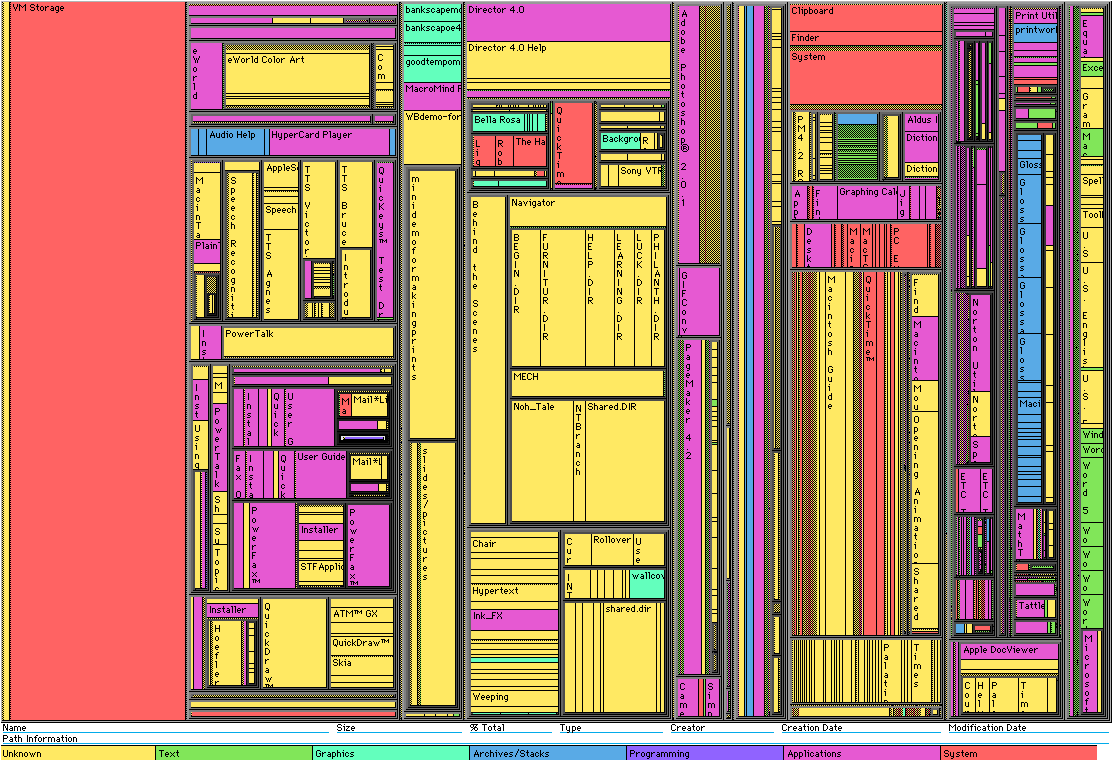
\includegraphics[width=.8\textwidth]{figures/intro/treemap_snd_colorful.png}
%     \caption{Earliest treemap method, Slice-and-Dice, displaying a file system.}
% \end{figure*}

\section{Visualizing temporal multidimensional data}
\label{sec:ch1_highdim}
%
Multidimensional (or high-dimensional) datasets have a number of observations (also called points or samples) where each observation has many attributes, also called variables, dimensions, or measurements. 
For datasets with relatively small numbers of observations and dimensions, techniques such as glyphs, parallel coordinate plots, table lenses, and scatterplot matrices can produce accurate and useful visual encodings.  
If a dataset has a large number of dimensions, roughly more than 4 to 5, however, multidimensional \emph{projections} tend to be the only scalable approach.  

Multidimensional projections take data in a high-dimensional space and project it into a lower-dimensional space, usually creating a 2D or 3D scatter plot, which we can directly visualize and reason about. In this transformation, the projection method attempts to create visual patterns that reflect the similarities or structure found in the high-dimensional space. That is, points which are similar -- according to any suitable similarity metric -- in the high-dimensional space are placed close in the 2D or 3D projection, and conversely.

Reflecting the similarities or structure found in the high-dimensional space can be interpreted in many ways, and the search for the ``best'' projection method has led to the proposal of a huge number of projection techniques.
There are many desirable traits projection methods can have, such as creating high distance or neighborhood preservation maps, scalability, simplicity, interpretability, out-of-sample capability, stability, and ease of use, among others. 
Optimizing a single one of these traits is already a challenging task that requires tradeoffs regarding the remaining traits. No single current method optimally satisfies all desirable requirements.

The trait that concerns us most in this thesis is \emph{stability}. Stability, or temporal coherence, needs to be taken into account when we project \emph{temporal} multidimensional data, that is, when the multidimensional data changes over time and, as illustrated in the previous section, we have multiple snapshots of the data. Most projection techniques are designed for static data. When used for time-dependent data, they usually fail to create a stable and suitable low dimensional representation. To follow the analogy with the dynamic treemaps discussed in Sec.~\ref{sec:ch1_tempo}: If we have a high-dimensional and temporal dataset, current projection methods usually create a visualization in which the observed points either do not change much while their corresponding high-dimensional counterparts change a lot; or they do change a lot whereas the high-dimensional data points only change little. Globally, the problem with projections is the same as that of treemaps -- they can produce false negatives and/or false positives which impair the ability of the user to judge about the data dynamics from seeing the visualization of the projected data.

\section{Temporal coherence}
\label{sec:ch1_coherence}
%
Treemaps and projections are incredibly useful techniques that, due to their compact and easy to interpret design, give unique insights into large and complicated datasets.
As mentioned so far, they were initially designed for static datasets. However, given the presence of dynamic datasets, the natural question arises on how to adapt them to handle such data, while avoiding the already discussed false-negative and false-positive problems. 

To illustrate the dynamic projections' instability, Fig.~\ref{fig:intro-pj-demo-instability} shows three different methods (G-PCA, TF-PCA~\citep{pca}, and TF-tSNE~\citep{tsne}) projecting the same dataset, using a trail-like visual encoding. The \emph{gaussians} dataset is a 100-dimensional dataset of 2000 samples covering 10 distinct isotropic Gaussian distributions that collapse into 10 single points over 10 timesteps. Knowing the dataset, we can tell that G-PCA renders quite faithfully the data dynamics and structure; TF-PCA creates an artificial amount of spiraling; and TF-tSNE creates a very large amount of apparently random and unstable motion that is not present in the data.  For the purpose of the illustration in Fig.~\ref{fig:intro-pj-demo-instability}, detailed knowledge of the G-PCA, TF-PCA, and TF-tSNE projection methods is not needed. The point being made is that different projection methods show widely different visual insights in the \emph{same} dataset. As such, they clearly cannot be all right -- raising the question of which method is the best and, subsequently, how to define what a good method is in this context.

% https://docs.google.com/drawings/d/1XENnHkpmsl6AqJfx5l2b-H4bSuKonbjgjYY_E599Q5c/edit
\begin{figure*}[h]
    \centering
    \includegraphics[width=\linewidth]{figures/projection-algorithm/demo-instability-trails-rebuttal-with-color-3.eps}
   %  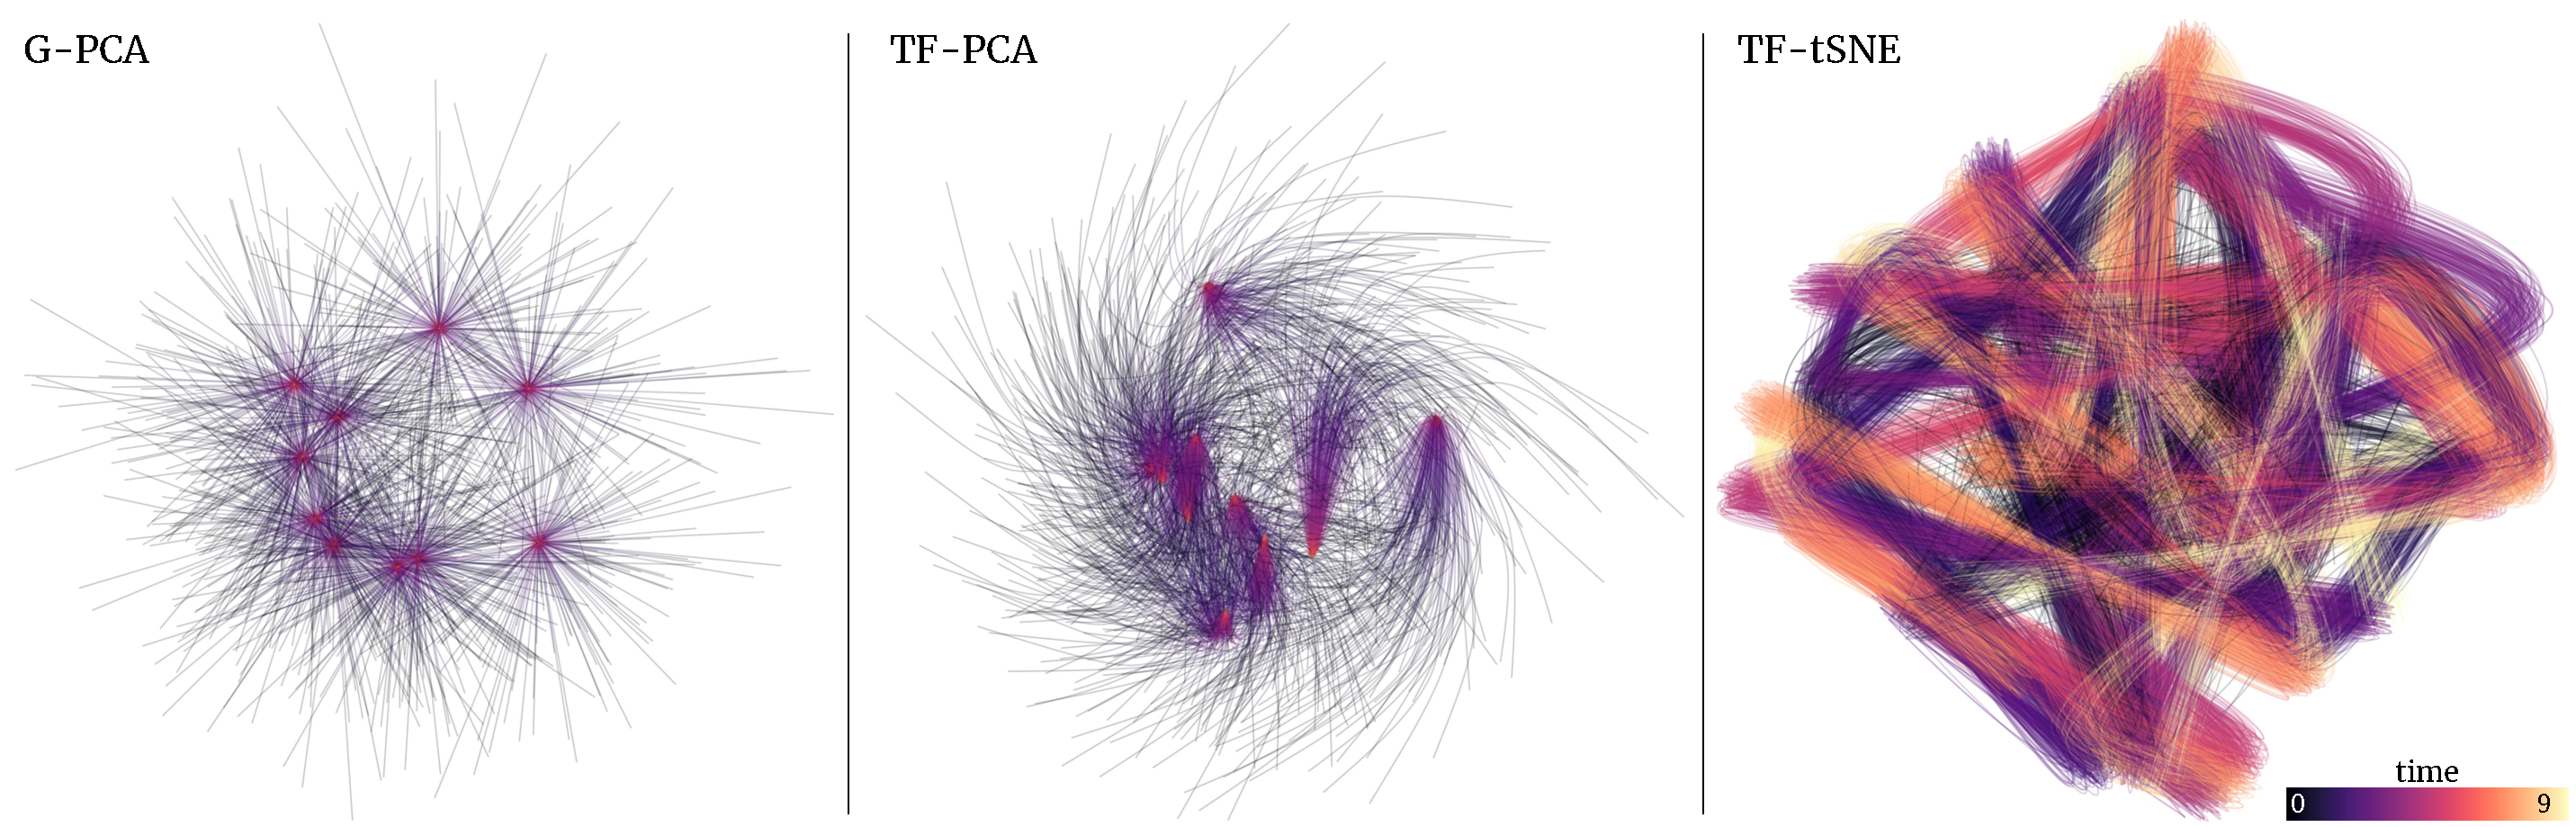
\includegraphics[width=0.48\linewidth]{figures/projection-algorithm/demo-instability-trails-rebuttal-with-color.pdf}
    \caption{A time-dependent collapsing 100-dimensional 10-Gaussian-distributions dataset (2000 points) from \cite{Rauber2016} is visualized by three projection methods. Point trails are colored by time (top) and class (bottom). The images show increasing amounts of instability artefacts.}
    \label{fig:intro-pj-demo-instability}
\end{figure*}

The same effect occurs when we create treemaps for time-dependent datasets. The top row of Fig.~\ref{fig:intro-tm-demo-instability} shows three snapshots/timesteps of the evolution of a simple weighted tree. The next two rows show two different treemapping algorithms creating rectangular treemap representations for the data (NMap and Squarified Treemap). Nmap creates a stable layout; that is, there are no significant changes in the positions of the cells driven by the small changes in the data, and the adjacencies in the layout remain the same over the evolution. In contrast, in the Squarified Treemap layout, cell \emph{d} (red) keeps changing its relative position. When dealing with more complicated datasets, this movement can happen for multiple cells simultaneously, making it impossible to accurately reason about the data and the change in the data. As for the projection example in Fig.~\ref{fig:intro-pj-demo-instability}, the issue is not understanding how NMap or Squarified Treemap work. Rather, the higher level question is that (at least) one of these methods is suboptimal, and, as a consequence, how to measure the quality of a dynamic treemapping method.

\begin{figure*}[h]
    \centering
    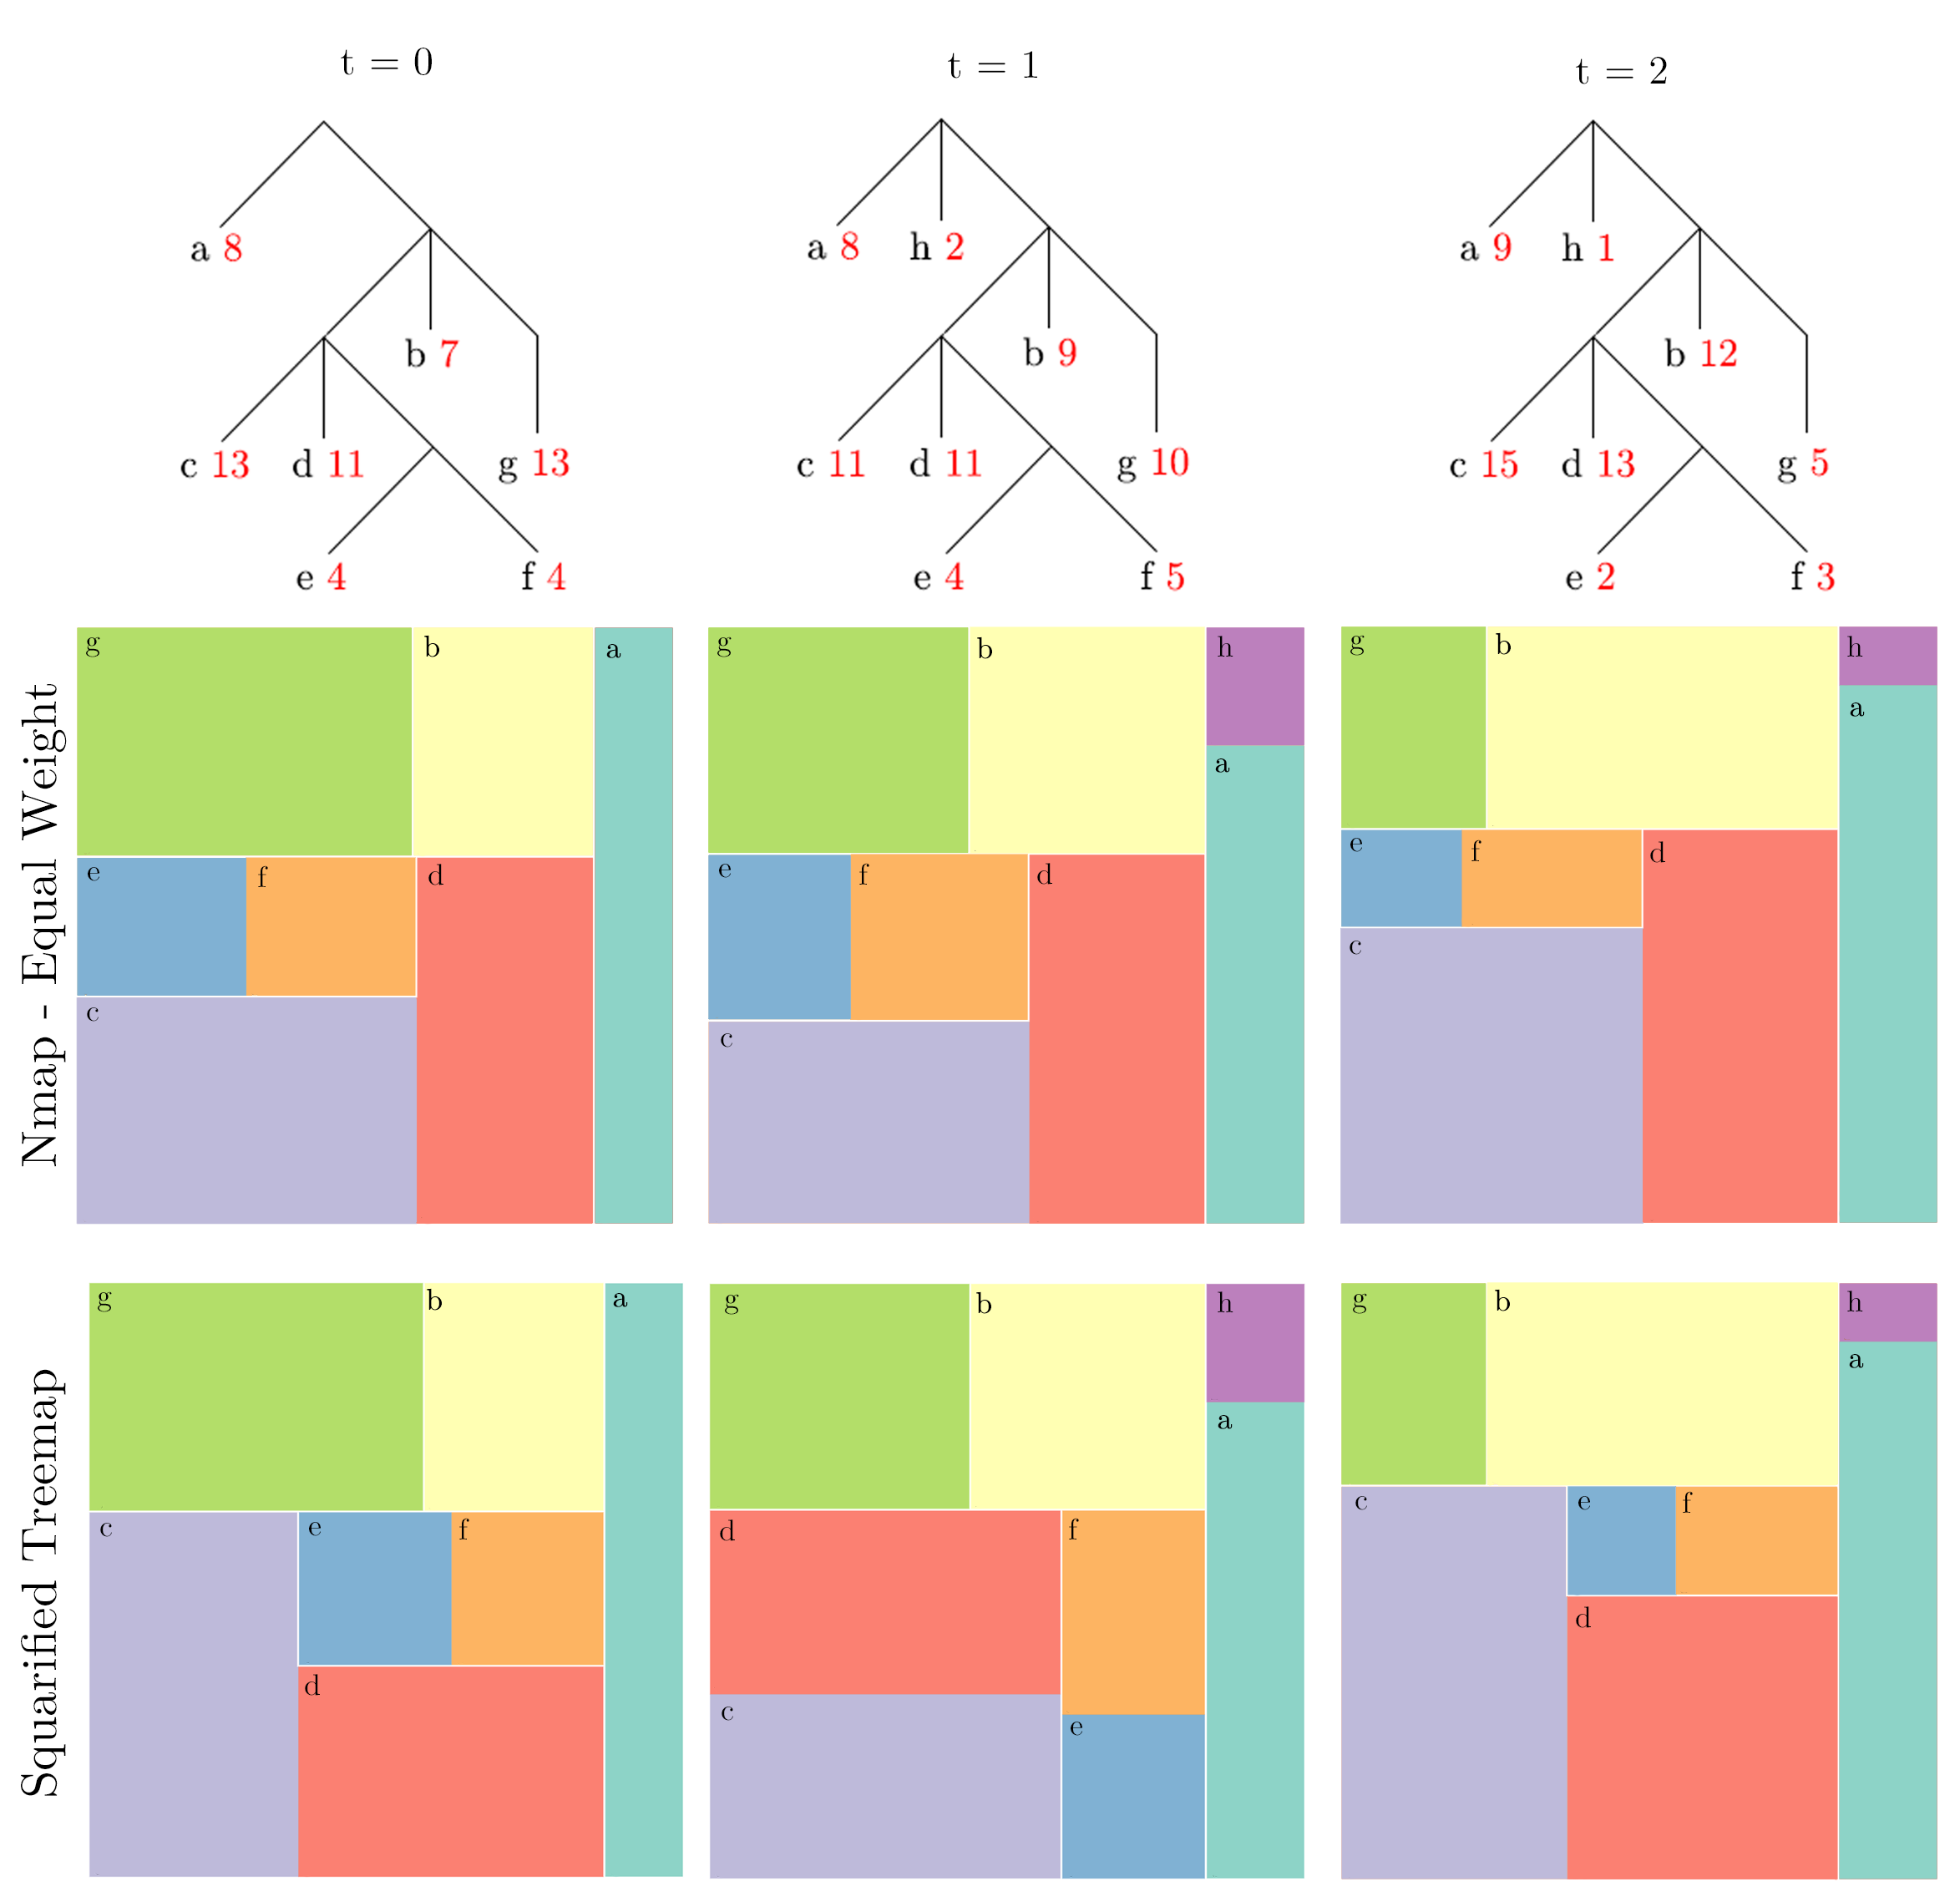
\includegraphics[width=\linewidth]{figures/intro/mov_sub_new.png}
    \caption{Layouts generated by NMap\,\citep{nmap} and Squarified Treemap\,\citep{sqr} for a sample hierarchical dataset
    of 3 time steps. We see how NMap is more stable, and similar in aspect ratio, than Squarified Treemap.}
    \label{fig:intro-tm-demo-instability}
\end{figure*}

To create faithful and useful representation of temporal data, we need to be able to ensure \emph{temporal coherence}: Small changes in the data should result in small changes in the visualization; large changes in the data should result in large changes in the visualization. All other mappings of changes in the data to changes in the visualization are arguably bad. Simply put, we want to guarantee that changes perceived by the viewer are due to changes in the data alone. However, while this 
desiderate is -- we argue -- clear and evident, there are no treemapping or projection algorithms that comply with it. Even more fundamentally, the very issue of relating data change to visualization change in these two contexts, and deciding what is a `good' mapping of the former to the latter, is not defined by theory or metrics to gauge it.

\section{Objectives and contributions}

We have argued that treemaps and projections are valuable tools for making sense of hierarchical and multidimensional data, respectively. However, when it comes to applying these visual encodings to \emph{time-dependent} data, these methods tend to show undesirable traits; and only limited research effort has been dedicated to understanding, testing, and developing methods that preserve temporal coherence. This research gap leads us to this thesis' high-level research question, stated next as

\subsection*{How to extend projections and treemaps to stably, accurately, and scalably handle temporal multivariate and hierarchical data?}

To address this question, there are three components that must be satisfied in either track. We must be able to

\subsection*{A. Develop ways of accurately measuring stability}

To evaluate the stability of a dynamic treemap or dynamic projection, we need to have reliable measurement tools that quantify the relationship between data change and visual change.

For treemaps, we developed the \emph{Unavoidable Change} \citep{vernier18software} metric, based on the mathematically proven minimum change that cells would need to undergo to accommodate the data change, and \emph{Baseline Treemaps} \citep{vernier_treemap}, a similar method to approximate the minimum amount of change that any time-dependent treemap must incur when data changes. We also proposed a set of stability metrics for dynamic projections based on the mathematics of visual quality metrics.
Before our work, there were no methods designed to measure instability that took into consideration data change -- they only looked at visual change, which can be deceiving. As such, we argue that our work provides a contribution to the fundamentals of using treemaps for reliably depicting dynamic hierarchical data.

\subsection*{B. Evaluate methods in the literature considering the tradeoff between stability and visual quality}

As already hinted, tens of methods for constructing treemaps and projections exist. However, and as also already hinted, few if none of these methods were gauged from the perspective of stability -- one reason thereof being the lack of a \emph{measure} for stability. Having developed such a measure, as mentioned above at point (A), we next use it to produce comprehensive evaluations for dynamic treemaps and projections from the stability perspective. Our contributions in this direction entail work along the following axes:

\begin{itemize}
    \item \emph{Metrics:} We proposed and implemented a novel set of metrics that reliably measures visual quality and stability.
    \item \emph{Datasets:} Since there was no previous extensive evaluation or benchmark designed for testing dynamic treemaps or projections, we collected and/or generated a comprehensive collection of datasets that drove our evaluations. 
    \item \emph{Methods:} Collection, implementation, and proposal of several dynamic treemap and projection algorithms. Most of the work on the topic up until our work was conjectural and not quantitatively tested.  Simply put, there was no central collection of algorithms that one could use to compare and gauge the performance of dynamic treemaps and dynamic projections. We claim that work solved a large part of this challenge.
    \item \emph{Analysis:} We combined the previous axes into comprehensive insights into dynamic projections and treemaps. Simply put, we generated quantitative and qualitative evidence showing how existing dynamic projection and treemap algorithms compare to each other, allowing both researchers and practitioners to choose which subset of algorithms are best suited to extend next, respectively directly use in practice.
\end{itemize}

\subsection*{C. Design state-of-the-art methods that strike a good balance between stability and visual quality}

Once the tools necessary to test and compare dynamic treemaps and projections were in place, we were able to leverage the gained insights to produce state-of-the-art algorithms that strike a better balance between stability and visual quality.

Specifically, we have developed Greedy Insertion Treemap (GIT) \citep{vernier18git}, a stable and scalable state-aware method for displaying dynamic treemaps. Compared to all treemapping algorithms that we were aware of at the time of GIT's development, we showed that GIT provides a better tradeoff between spatial quality and stability, therefore surpassing its competitors. Moreover, GIT is simple to implement, generic, and computationally scalable.

Regarding projections, we proposed PCD-tSNE and LD-tSNE \citep{Vernier2021}, two neighborhood-based projection methods that use global guides to steer the projected points. This avoids unstable movement that does not encode data dynamics while keeping, at the same time, the highly praised visual quality of the t-Stochastic Neighborhood Embedding (t-SNE) projection method\,\citep{tsne}, arguably the best known high-quality projection method used nowadays for high-dimensional data. As for GIT, PCD-tSNE and LD-tSNE are generic methods, with good computational scalability.

\bigbreak

Lastly, it is important to mention that all aspects of our research are open. All the code and data is organized and available online to facilitate further research on dynamic treemaps and projections. This directly supports our answering of the earlier mentioned research questions -- which, besides theory, require materials such as data and software for interested researchers and practitioners to replicate, extend, and ultimately use our contributions.

\section{Organization of the thesis}

\alex{Here and later: I added cite{xxx} reference placeholders for the obvious things - like the 1st time you refer to a term or method. Please fill these in. It's trivial to do so. Will add more as I read/correct more Please pedantically fill these in!}

\eduardo{will add refs later}

\alex{Yes please do. Also, in sec 1.5, be short: simply list the chapters and say what you do in which and how that relates to what PREVIOUS sections in this chapter mention. Easy. Just, like, 1..2 paragraphs per chapter, not more.}

\eduardo{(explanation for unavoidable change metric is not in the text yet -- software visualization paper)}

\eduardo{quotes come from here http://www.cs.umd.edu/hcil/treemap-history/index.shtml}


\chapter{Treemap Evaluation for Software Evolution Data}
\label{ch:soft-eval}
\blfootnote{This chapter is based on the paper ``Quantitative Comparison of Dynamic Treemaps for Software Evolution Visualization'' \citep{vernier18software}}
% \title{Quantitative Comparison of Dynamic Treemaps for Software Evolution Visualization}

\textit{
As outlined in Chapter \ref{ch:intro}, one of our two research questions concerns how to extend treemapping algorithms to handle time-dependent hierarchical data. To do this, we need first and foremost to understand how existing treemapping algorithms fare when displaying dynamic data. In more detail, we also need to know how to quantitatively compare such algorithms. In this chapter, we address the above two questions by a first evaluation. For this, we consider a smaller scope in terms of datasets, focusing on dynamic hierarchies coming from evolving software repositories. Using this limited scope of datasets, and beyond evaluating existing treemapping algorithms, we introduce a stability metric for gauging the performance of such algorithms in the presence of time-dependent data, that quantifies the relationship between data change and change in the data's visualization using treemaps. We next extend this approach in Chapter \ref{ch:tree-eval} to reliably and fairly test treemapping algorithms on generalized data, \emph{i.e.}, a large number of datasets from different sources, displaying a variety of traits and dynamics, beyond dynamic hierarchies coming from software evolution.}


\vspace{5mm} %5mm vertical space

\noindent \textbf{Abstract:}
Dynamic treemaps are one of the methods of choice for displaying large hierarchies that change over time, such as those encoding the structure of evolving software systems. While quality criteria (and algorithms that optimize for them) are known for static trees, far less has been studied for treemapping dynamic trees. We address this gap by proposing a methodology and associated quality metrics to measure the quality of dynamic treemaps for the specific use-case and context of software evolution visualization. We apply our methodology on a benchmark containing a wide range of real-world software repositories and 12 well-known treemap algorithms. Based on our findings, we discuss the observed advantages and limitations of various treemapping algorithms for visualizing software structure evolution, and propose ways for users to choose the most suitable treemap algorithm based on the targeted criteria of interest.

\section{Introduction}
\label{sec:treemap_eval_intro}
%
Hierarchies play a central role in understanding large software systems. Such systems evolve over hundreds of revisions or more, and can have thousands of elements or more, which are typically organized hierarchically (\emph{e.g.} in folders, files, classes, and methods). Hence, tools for visually understanding evolving hierarchies are a key component in the program comprehension arsenal. Treemaps are a well known method for visualizing hierarchical data. Given an input tree whose leafs have several attributes, treemaps recursively partition a 2D spatial region into cells whose area, color, shading, or labels encode the tree's data attributes. Compared to other methods such as node-link~\citep{harel,frick} or Sunburst~\citep{sunburst,sunburst2} techniques, treemaps use all available screen pixels to show data and thus can handle trees of tens of thousands of nodes.

\emph{Dynamic} treemaps leverage the above advantages to show dynamic, or evolving, trees. Given a tree sequence, they create an animated sequence of treemap layouts that reflect how the structure and attributes of the trees in the sequence change in time. Evolving treemaps have been created both by using classical static treemap algorithms~\citep{treevis} or by specialized algorithms~\citep{sondag17,hees17,hahn10}.

Evolving treemaps have received great interest in software visualization\,\citep{diehl08,hees17,hahn10,fisher10,gotz11}. As many treemap techniques exist, the question emerged of how to measure their quality. For common rectangular treemaps, which map tree nodes to rectangles, visual quality is typically measured by the aspect ratio of these rectangles. However, the aspect ratio may not capture all desirable qualities of such treemaps. For example, bad aspect-ratio cells of a tiny area could influence the overall visual quality far less than large bad aspect-ratio cells. Atop visual quality, evolving treemaps are assessed by measuring their rate of visual change. However, this metric may not capture all desirable properties: Large visual changes in a treemap are expected (and actually desirable) when the underlying tree changes drastically, but undesired when the tree changes only slightly.

Although treemaps are used for over two decades in software visualization~\citep{shneiderman92,schulz11_treesurvey,treevis,landesberger11}, there are few comprehensive evaluations of the quality of dynamic treemap techniques and, to our knowledge, none that focuses on trees capturing software evolution. The aim of this chapter is to fill this gap. For this, we first review the related work in (dynamic) treemaps and their quality measurement, with a focus on software visualization (Sec.~\ref{sec:init-background}). We next refine desirable treemap properties into 5 quality metrics that capture both spatial quality and dynamic quality (Sec.~\ref{sec:init_metrics}). We measure these metrics on 12 well-known treemap algorithms on 28 tree sequences, ranging from a few hundred to tens of thousands of elements, all extracted from software repositories. We next visualize and analyze our results to address questions that practitioners would like to answer to choose a suitable technique (Sec.~\ref{sec:mat_aggr}). We discuss our findings and proposed methodology in Sec.~\ref{sec:init-discussion}. Our results (datasets, metrics, treemap implementations, evaluation results, and visualizations thereof) are publicly accessible for researchers in the software visualization field interested in evaluating treemap methods for evolving software hierarchies.

\section{Background}
\label{sec:init-background}
%
%
Hierarchies are arguably the central element in most software visualizations. They capture the physical (\emph{e.g.} files and folders) or logical software (\emph{e.g.} syntax tree) system structure, together with static or dynamic attributes, \emph{e.g.}, code size, quality metrics~\citep{lanza06}, change requests, or testing results~\citep{diehl08}. Both static and dynamic hierarchies in program comprehension are typically extracted by mining software repositories~\citep{lanza03,kagdi07}.
When small (a few hundred nodes), such trees can be visualized using classical node-link layouts such as in class or architecture diagrams~\citep{muller88,lanza03,telea02}. This works well for architecture-level views on a software system. However, code-level views, which contain nodes from subsystems all the way to classes and methods, generate large trees, having hundreds of thousands of nodes\,\citep{sunburst2}. These require space-filling methods, such as icicle plots~\citep{holten06,cornelissen07} or, the method of choice, treemaps. The latter are discussed below.

\subsection{Treemap algorithms}
%
%
Let $T=\{n_i\}$ be a tree with nodes $n_i$, and let $a_i \in \mathbb{R}^{+}$ be an attribute defined on the tree leaves. For non-leaf nodes $n_i$, $a_i$ equals the sum of the attributes of the children of $n_i$. A rectangular treemap algorithm $TM$ creates a set of rectangle cells $\{c_i\} = TM(T)$, $c_i \subset \mathbb{R}^2$ for the nodes $n_i$ so that the area of $c_i$ equals $a_i$ and children node cells create a partition of their parent cell. Several treemap algorithms exist, as follows (for detailed surveys, see\,\cite{schulz11_treesurvey,hci_treemaps,treevis,landesberger11}). Slice and dice (SND) treemaps pioneered the concept but were found to create too long-and-thin cells which are hard to grasp\,\citep{shneiderman92}. Subsequent algorithms tried to improve this aspect, quantified by the aspect ratio (AR) of the treemap cells. Squarified treemaps (SQR) propose a slicing heuristic that achieves, in general, very good (close to one) AR values~\citep{sqr}. Nagamochi and Abe refined this idea in an algorithm (APP) that approximates the optimal AR a given treemap can reach~\citep{nagamochi07}. However, SQR is not particularly \emph{stable} -- small changes in the input tree can yield large changes in the treemap layout. Several algorithms have aimed to improve stability. Ordered treemaps (OT)~\citep{ordered} and Strip treemaps (STR)~\citep{bederson02} lay out cells $c_i$ to follow a predefined order of the nodes $n_i$. Different algorithms propose different orderings: Pivot-by-Middle (PBM), Pivot-by-Size (PBZ), and Pivot-By-Split-Size (PBS)~\citep{ordered}; Engdahl's Split algorithm~\citep{engdahl}; and laying out cells along a space-filling curve, \emph{e.g.}, Spiral (SPI)~\citep{spiral}, and Hilbert (HIL) and Moore (MOO) fractal curves~\citep{hilbert_moore}. Spatially-Ordered Treemaps (SOT)~\citep{sot} extend SQR by ordering sibling nodes so that the most similar ones are processed in turn. NMap~\citep{nmap} uses a related idea; cells are placed according to the similarity of their attributes, using a dimensionality-reduction approach. Two versions exist: NMap Alternate Cuts (NAC) alternate horizontal and vertical cuts to subdivide the space (akin to SND), while NMap Equal Weights (NEW) splits the space to create similar-size cells. However, NMap was only applied to single-level trees. Recently, Sondag \emph{et al.} proposed stable treemaps~\citep{sondag17}, which aim to improve both the AR and stability for dynamic treemaps by using non-sliceable layouts.

Other cell shapes can be used besides rectangles. Voronoi treemaps~\citep{balzer05,balzer05b} exploit the properties of weighted Voronoi diagrams to create organic-looking visualizations where cells are convex polygons with, in general, good AR values. Voronoi methods have also been used, with good results, to construct dynamic treemaps for visualizing software structure evolution~\citep{hees17,gotz11}. Hybrid treemaps (HTM)~\citep{htm} combine various basic treemap techniques to generate the final layout. Other variants include jigsaw treemaps~\citep{jigsaw}, orthoconvex treemaps~\citep{deberg14}, and bubble treemaps~\citep{bubble}.

\subsection{Treemap quality metrics}
\label{sec:quality}
%
%
In practice, the quality of treemaps is measured using two types of metrics, as follows.

\noindent\emph{Spatial quality} metrics capture how easy one can read the information shown in a static treemap. Such metrics include the aspect ratio (AR) of the treemap cells, which ideally should equal one. For ordered treemaps, the readability metric measures how often one switches visual scanning direction while reading the treemap in order~\citep{bederson02}; and the continuity metric measures how often cells for neighbor nodes (following the given node order) are not neighbors in the treemap layout~\citep{spiral}.\\

\noindent\emph{Stability} metrics capture how easy one can follow the changes in a dynamic treemap. Given two  treemaps for two (typically consecutive) time-moments $t_i$ and $t_j$, \cite{ordered} define stability as the distance between the vectors $(x_k(t_i), y_k(t_i), w_k(t_i), h_k(t_i))$ and $(x_k(t_j), y_k(t_j), w_k(t_j), h_k(t_j))$, where $x$ and $y$ are the coordinates of the top-left corner, and $w$ and $h$, the width, and the height of a cell $c_k$, averaged over all cells in the treemap.
\cite{hahn10} use for stability the change of distance between the centroids of $c_k(t_i)$ and $c_k(t_j)$, averaged over all cells.
\cite{hilbert_moore} use the same cell-change metric (top-left corner, width, height) as \cite{ordered}, but aggregate via variance rather than average. They also propose a drift metric which measures how much a cell moves away from its average position over a time period. Two recent metrics measure stability at the level of pairs of cells rather than individual cells. \cite{Hahn2017} propose the relative direction change, which measures the angle change of centroids for every pair of cells in a layout. \cite{sondag17} measure the relative position change of each cell with respect to eight planar zones defined by four lines given by the edges of that cell, averaged over all treemap cells.

%ALEX: I didn't cite our EuroVis poster here since it doesn't introduce any new metrics as such

\subsection{Software visualization challenges}
\label{sec:current_state}
%
%
Summarizing, considerable effort went into designing static treemap methods and measuring their quality. Less effort went to evaluating dynamic treemaps. We identify limitations in several directions, with a focus on our use-case of visualizing large evolving software hierarchies:\\

\noindent\textbf{Algorithms:} Treemap papers typically compare a few (2--5) algorithms from the much larger set of available ones. In particular, it is not clear how most existing static treemap algorithms perform on the types of dynamic trees extracted from software evolution analyses.\\

\noindent\textbf{Datasets:} Existing methods are typically evaluated on one or a few datasets. While in this chapter, we cannot (and do not aim to) cover the full space of all possible trees, we can do better than existing work: For our specific context of software visualization, we aim to know how treemap methods perform on a representative collection of software hierarchies capturing software evolution.\\

\noindent\textbf{Metrics:} As outlined in Sec.~\ref{sec:quality}, stability is currently measured by looking at how much two treemaps (typically for consecutive time moments) change with respect to each other. However, when the underlying tree sequence changes a lot, \emph{e.g.} by insertions or deletions of many files or classes at the same moment during a software repository's evolution (an event well-known to take place often in software evolution), the treemap will change a lot, so its evolution will be labeled as unstable. However, it is actually \emph{desirable} to have a large visual change in this case, as this correctly shows the presence of a large data change. We argue that ways to measure stability as a function of the data change are needed.\\

\noindent\textbf{Result exploration:} Most evaluations consider only aggregated metrics with one value per technique or per technique-and-dataset. Analyzing the actual distribution of metric values over both layout-space and time can give extra insights into the strengths and weaknesses of specific techniques.\\

\noindent\textbf{Replicability:} Treemap evaluations can be hard to replicate as datasets and algorithm implementations are not always openly available or not integrated to make a comparison on different datasets, and along different metrics, easy. Replicability is a growing concern in information visualization but with particular weight in software visualization\,\citep{sensalire09,seriai14,merino18}.

The remainder of this chapter is dedicated to addressing the above points.


\begin{table}[htbp!]
\small
\centering
\scalebox{0.9}{
\begin{tabular}{|l|l|r|r|}
\hline
\textbf{Dataset} & \textbf{Revisions} & \textbf{Nodes (total)} & \textbf{Average depth} \\
\hline
animate.css & 50 & 3454 & 2.87\\
AudioKit & 22 & 11178 & 6.95\\
bdb & 62 & 2658  & 3.83\\
beets & 106   & 9844 & 3.75\\
brackets &  88  & 120292 & 12.85\\
caffe & 44 & 12969   & 4.93\\
calcuta & 50 & 2882 & 10.76\\
cpython   & 321 & 584821 & 6.50\\
earthdata-search   &  46& 18539 & 6.82\\
emcee & 64 & 1746  & 3.62\\
exo & 97 &  36436  & 11.88\\
fsharp   & 69 & 22906 & 7.89\\
gimp   & 72 &  170418 & 5.19\\
hospitalrun-frontend   & 38 &  16759 & 5.71\\
Hystrix & 61 & 15530  & 13.29\\
iina & 74 &  6849  & 4\\
jenkins & 137  & 277185 & 11.94 \\
Leaflet &  84  & 13381 & 4.86 \\
OptiKey   & 36 & 9782 & 6.72\\
osquery  & 37 & 14111 & 5.75 \\
PhysicsJS   & 20 & 2022 & 4.6\\
pybuilder   & 53 & 5457 & 7\\
scikitlearn   & 88 & 48468 & 5.75\\
shellcheck   & 53 & 746 & 2.39\\
soundnode-app   & 35 & 3196 & 6.88\\
spacemacs   & 51 & 10201 & 4.96\\
standard   & 29 & 203 & 2\\
uws & 122 & 4093 & 2.76\\
\hline
\hline
\textbf{Totals:} & 2132 & 1458036 & 5.77\\
\hline
\end{tabular}
}
\caption{Software evolution tree datasets used in the evaluation.}
\vspace{-0.2cm}
\label{tab:software_datasets}
\end{table}

\begin{figure*}[htbp!]
\centering
\includegraphics[width=\textwidth]{figures/initial-treemap-evaluation/datasets.eps}
\caption{Union trees of software evolution tree datasets used in the evaluation. Names correspond to public repositories on GitHub.}
\label{fig:datasets}
\end{figure*}


\section{Measuring the quality of dynamic treemaps}
\label{sec:init_metrics}
%
%
To address the current limitations of dynamic treemap evaluations in software visualization, we performed an in-depth study covering the five directions in Sec.~\ref{sec:current_state}, as follows.

\subsection{Algorithms}
\label{sec:mat_algos}
%
We consider in our evaluation 12 methods: Approximate (APP), Hilbert (HIL), Moore (MOO), NMap-Alternate-Cuts (NAC), NMap-Equal-Weights (NEW), Pivot-by-Middle (PBM), Pivot-by-Size (PBZ), Pivot-by-Split-Size (PBS), Slice-and-Dice (SND), Spiral (SPI), Squarified (SQR), and Strip (STR) treemaps. For NMap, we use as seed layout the one computed by SQR (for details, see\,\cite{nmap}). We do not consider non-rectangular treemap methods, as their quality is less easy to compare with rectangular ones, and are also less used in practice. Also, we do not consider the stable treemaps in~\citep{sondag17} as this method is considerably slower (over one order of magnitude) than the above-mentioned methods.

\subsection{Datasets}
\label{sec:mat_data}
%
We evaluate all above treemap methods on a collection of 28 datasets (Tab.~\ref{tab:software_datasets}). All of them consist of trees describing the hierarchy of public and well-known GitHub software repositories (folders, files, classes), one tree per revision, where leaves (classes) are attributed by their number of lines of code. The trees and their attributes have been extracted from the actual repositories by a fully automatic pipeline we built using \emph{libgit2}\,\citep{libgit2} for repository parsing and Understand\,\citep{understand} for code analysis. For a more detailed description of the extraction pipeline, we refer to~\cite{vmv}. The respective software projects have widely different sizes, tree depths and structures, durations, numbers of contributors, language (C, C++, Java, Python), and code type (library, framework, application). This is seen in the figures in Tab.~\ref{tab:software_datasets} and also in Fig.~\ref{fig:datasets} which shows the union trees $\cup_{i} T(t_i)$ for the considered datasets. Hence, we argue that this collection covers reasonably well the space of tree sequences obtained from software evolution.

\subsection{Metrics}
\label{sec:mat_metrics}
%
Let $w_k$ and $h_k$ be the width and height of cell $c_k$; and $(W,H)$ the width and height of the screen space we draw the treemap in. With these, we consider the following metrics.

\subsubsection{Spatial quality metric}
\label{sec:mat_met_spatial}
%
We first consider the classical aspect-ratio metric
%
\begin{equation}
Q^{AR}_k = \min(w_k,h_k)/\max(w_k,h_k).
\label{eqn:spatial_ratio}
\end{equation}
%
Introduced in~\cite{sqr}, this metric has been since then used by all treemap evaluations to capture spatial quality. As such, we keep it in our evaluation. It is designed to give high scores for rectangles with sides of similar length, and low scores otherwise.
%

\subsubsection{Stability metrics}
\label{sec:mat_met_stab}
%
Let $c_k(t_i)$ and $c_k(t_j)$ be two cells in two consecutive versions $T(t_i)$ and $T(t_j=t_{i+1})$ for the same node in a dynamic tree. Typical stability metrics (Sec.~\ref{sec:quality}) only measure the \emph{visual} change $\delta c_k$ between $c_k(t_i)$ and $c_k(t_j)$. We use for $\delta c_k$ the average sum of distances between the four corresponding corners of $c_k(t_i)$ and $c_k(t_j)$~\citep{ordered}, normalized by the treemap diagonal $\sqrt{W^2+H^2}$, so $\delta \in [0,1]$. We next define the \emph{data change} between nodes $n_k(t_i)$ and $n_k(t_j)$ as $\delta a_k = |a_k(t_i)-a_k(t_j)|$, where $a_k$ is the relative weight of $n_k$ at time $t_i$. If either of $n_k(t_i)$ or $n_k(t_j)$ does not exist, \emph{i.e.}, a node was created or deleted in versions $t_i$ or $t_j$, we set the respective $a_k$ to zero, which is as if the respective node was depicted by a zero-size cell. We normalize $a_k(t_i)$ by the weight sum of all nodes $n_k$ present at time $t_i$, so $\delta a_k \in [0,1]$. With this, we define the stability of a cell $c_k$ in a treemap in several ways. First, we define stability as
%
\begin{equation}
Q^{RATIO}_k =  (1-\delta c_k) / (1 - \delta a_k).
\label{eqn:stab_ratio_1}
\end{equation}
%
When visual changes are proportional to data changes, since both are normalized, $Q^{RATIO}_k$ goes to one. Note that an analogy to Eqn.~\ref{eqn:spatial_ratio}, \emph{i.e.}, $Q^{RATIO}_k=\min(\delta c_k, \delta a_k)/\max(\delta c_k, \delta a_k)$ does not work: Eqn.~\ref{eqn:spatial_ratio} is symmetric in width and height. For stability (Eqn.~\ref{eqn:stab_ratio_1}), we want to assess visual change as a function of data change, and not conversely.

\noindent A second way to define stability is by
%
\begin{equation}
Q^{MOD}_k = 1 - | \delta c_k - \delta a_k |.
\end{equation}
%
For proportional visual \emph{vs} data changes, $Q^{MOD}_k=1$.

\begin{figure}[htbp!]
\centering
\includegraphics[width=.6\textwidth]{figures/initial-treemap-evaluation/unavoidable.eps}
%\includegraphics[width=1.0\linewidth]{figures/unavoidable.eps}
\vspace{-0.1cm}
\caption{Computation of unavoidable change metric $Q^{UNAV}_k$.}
\vspace{-0.2cm}
\label{fig:unavoidable}
\end{figure}


%\noindent We compute ($Q_k^{RATIO}$ and $Q_k^{MOD}$) and area-weighted ($Q_k^{WRATIO}$ and $Q_k^{WMOD}$) versions of the above metrics, like in Eqn.~\ref{eqn:spatial_weighted}. For a whole tree, we average per-cell metrics, like for spatial metrics (Sec.~\ref{sec:mat_met_spatial}). }

To compare data and visual changes, $Q_k^{RATIO}$ and $Q_k^{MOD}$ must be normalized to the same range, therefore we clip $Q_k^{RATIO}$ to the $[0,1]$ interval. However, this can introduce normalization biases, \emph{e.g.} when the data changes and visual changes have very different ranges. To address this, we next propose to define stability purely in visual space. For this, we consider the actual change $\delta c_k$ of a cell \emph{vs} the \emph{unavoidable}, \emph{i.e.} minimal, change $\Delta c_k$ that $c_k$ would need to undergo to accommodate the data change from $a_k(t)$ to $a_k(t+1)$. If $\delta c_k > \Delta c_k$, the algorithm is unstable; if $\delta c_k = \Delta c_k$, it is fully stable. We compute $\Delta c_k$ as follows (Fig.~\ref{fig:unavoidable}). Let $c_k(t)$ be a cell of width $w$ and height $h$ at time step $t$. Let $c_k(t+1)$ be the version of $c_k(t)$, of area $a_k(t+1)$, at step $t+1$. We first note that $\delta c_k$ is minimal when $c_k(t)$ and $c_k(t+1)$ have the same center, as visual change is then caused \emph{purely} by data change and not by avoidable `drift' of the cell corners. Taking a $xy$ coordinate frame centered in this common cell center, the top-right corner of $c_k(t)$ is constrained to a hyperbola $y = a_k(t+1)/4x$. Hence the minimal change $\Delta c_k$ is four times the minimal distance $D$ from this corner to the hyperbola, \emph{i.e.}
%
\begin{equation}
D(x) = \sqrt{(x - w/2)^2 + (a_k(t+1)/4x - h/2)^2}. \nonumber
\end{equation}
%
To find the minimum of $D$, we solve $\frac{d D^2}{d x}=0$ for $x \geq 0$. This quartic equation in $x$ has analytic solutions. We obtain $x$, the width of the optimal cell $c_k(t+1)$, and thereby the minimal $\Delta c_k$. We define the unavoidable-motion stability as
%
\begin{equation}
Q^{UNAV}_k = 1 - (\delta c_k - \Delta c_k).
\end{equation}
%

Finally, we define stability for a whole tree $T$ as the \emph{absolute} value of the Pearson correlation coefficient
%
\begin{equation}
Q^{CORR} = \left| \frac{  \sum_k (\delta c_k - \overline{\delta c_k}) (\delta a_k - \overline{\delta a_k})  } {\sqrt { \sum_k (\delta c_k - \overline{\delta c_k})^2} \sqrt { \sum_k (\delta a_k - \overline{\delta a_k})^2}   }\right|
\label{eqn:pearson}
\end{equation}
%
of the signals $\{\delta c_k\}$ and $\{\delta a_k\}$ for all cells $c_k \in T$, where $\overline{\delta c_k}$ and $\overline{\delta a_k}$ are the signals' averages, so $Q^{CORR} \in [0,1]$. If visual and data changes $\delta c_k$ and $\delta a_k$ are linearly correlated, $Q^{CORR}$ reaches one. $Q^{CORR}$ close to zero indicates uncorrelated changes, \emph{i.e.}, instability.

\noindent Compared to existing treemap stability metrics~\citep{ordered,hahn10,hilbert_moore,sondag17}, all our above metrics consider the \emph{relation} of visual change $\delta c_k$ to data change $\delta a_k$. This is a fundamental difference: A treemap method $TM(T) = \{c_i\}$ is a \emph{function} from trees $T$ to cell-sets $\{c_i\}$, so its stability should be defined akin to Cauchy or Lipschitz continuity, which relate function-value ($\{c_i\}$) changes to variable ($T$) changes rather than measuring function changes only. Indeed: If a function's output strongly changes, the function \emph{itself} is not necessarily unstable; this can happen when the input variable strongly changes.

\subsubsection{Metric weighting}
%
As mentioned in Sec.~\ref{sec:treemap_eval_intro}, very small but bad aspect-ratio cells may not strongly influence the overall perceived spatial quality of a treemap, since they are barely visible. The same argument could be made for very small unstable cells \emph{vs} the overall perceived stability. To model these, when computing the average value of the metrics $Q^{AR}$, $Q^{RATIO}$, $Q^{MOD}$, and $Q^{UNAV}$, we weigh the respective per-cell values $Q^{AR}_k$ (and the other three ones) by the sizes $a_k$ of their cells. We used such weighted metrics in all experiments described next in Secs.~\ref{sec:q2}-\ref{sec:q4}. However, the obtained results showed that the aggregated weighted metric values differ only very slightly from their unweighted versions. As such, in the following we will only consider the unweighted metric versions.


\section{Result exploration}
\label{sec:mat_aggr}
%
We measure the five metrics (Eqns.~\ref{eqn:stab_ratio_1}-\ref{eqn:pearson}) on all 28 test datasets (Sec.~\ref{sec:mat_data}) processed by all 12 treemap methods (Sec.~\ref{sec:mat_algos}). We record metrics at the \emph{cell} level (except $Q^{CORR}$, recorded at tree level). This yields a high-dimensional-and-hierarchical dataset, conceptually a
 table with seven columns (5 metrics, algorithm ID, dataset ID, time step) and as many rows as the number of measured cells in all datasets, all timesteps. Exploring this data space is a challenge in itself. As noted in Sec.~\ref{sec:current_state}, current treemap evaluations typically present only a few metrics, aggregated to a single (typically average) value per algorithm or per algorithm-and-dataset. To get more insight, we propose several visualizations that present various aspects of the evaluation data to answer specific questions concerning the evaluated algorithms. We proceed in a bottom-up fashion: We first explore the data at the finest (cell) level-of-detail (Sec.~\ref{sec:q1}). This shows subtle differences between different methods (we show all table rows), but cannot show all evaluated metrics (table columns). Next, we study the quality as a function of time, for one given evolution sequence (Sec.~\ref{sec:q2}). Thirdly, we compare the aggregated 5 metrics for all dataset and algorithm combinations (Sec.~\ref{sec:q3}). Finally, we aggregate all results to present a compact comparison of all algorithms (Sec.~\ref{sec:q4}).

\subsection{How does visual change relate to data change (Q1)?}
\label{sec:q1}
%
%
Before actually evaluating stability, we want to study the distribution of visual changes created by the tested algorithms as function of the respective data changes for all datasets, all timesteps. For this, we show a scatterplot per algorithm (Fig.~\ref{fig:scatterplot}), where, for all datasets, $x$ maps $\delta a_i(t_j)$, \emph{i.e.} data change of all cells $c_i$ from time step $t_j$ to $t_{j+1}$, for all time steps $j$; and $y$ maps $\delta c_i(t_j)$ (see Sec.~\ref{sec:mat_met_stab}). A point is thus a cell in a revision of a dataset. To account for overplotting, we compute density maps from these scatterplots using kernel density estimation\,\citep{kde} and color-code the density using a heat colormap.
%
\begin{figure}[htbp!]
\centering
\includegraphics[width=.93\linewidth]{figures/initial-treemap-evaluation/scatterplots.eps}
\vspace{-0.2cm}
\caption{Correlation of data and visual change per algorithm, all datasets.}
\vspace{-0.1cm}
\label{fig:scatterplot}
\end{figure}
%
Ideally, the visual change should be proportional to data change (Sec.~\ref{sec:mat_met_stab}), so our scatterplots should be close to a diagonal line. We see that this is not the case. All plots show an upwards-pointing `tail' close to the origin. This tells that most cells with small data changes have disproportionately large visual changes, so instability affects more the small than the large cells. Shallower tails indicate more stable methods, \emph{e.g.} SND. To get a more summarized insight, we also plot a linear-regression line (red), characterized by the slope ($\alpha$) and the $y$-intercept ($\beta$), and compute the linear correlation coefficient ($r$) and standard error ($s_e$) of the points. Larger $r$ coupled with small $s_e$ values indicate methods which correlate visual change with data change better, \emph{e.g.} SND and NAC. We also find the worst-correlating methods, SQR and PBS, and see that SQR is about 7 times worse than SND.

\subsection{How is quality evolving in time (Q2)?}
\label{sec:q2}
%
%
Q1 does not show how quality fluctuates over time for a given tree sequence. Knowing this is important to assess what one can expect when using a given treemap algorithm for a sequence of hundreds of revisions extracted from a repository. To assess this, we show a chart per method, per dataset, and per metric family (that is, spatial quality $Q^{AR}$ and per-timestep averaged values of the four stability metrics $Q^{RATIO}$, $Q^{MOD}$, and $Q^{UNAV}$). In all charts, $x$ maps time and $y$ shows a box plot indicating median (black), 25-75\% range (green), and 5-95\% range (gray). Since we 
cannot show this chart for all our 28 datasets (nor can we aggregate them in a single chart), we select one representative dataset to depict: \emph{cpython}. The dataset was extracted from the official Github repository hosting the source code of the Python programming language\,\citep{cpython}. This is our largest dataset with 321 revisions and an average of over two thousands tree nodes per revision. Results for other datasets can be found online\,\citep{benchmark}.

\begin{figure*}[htbp!]
\centering
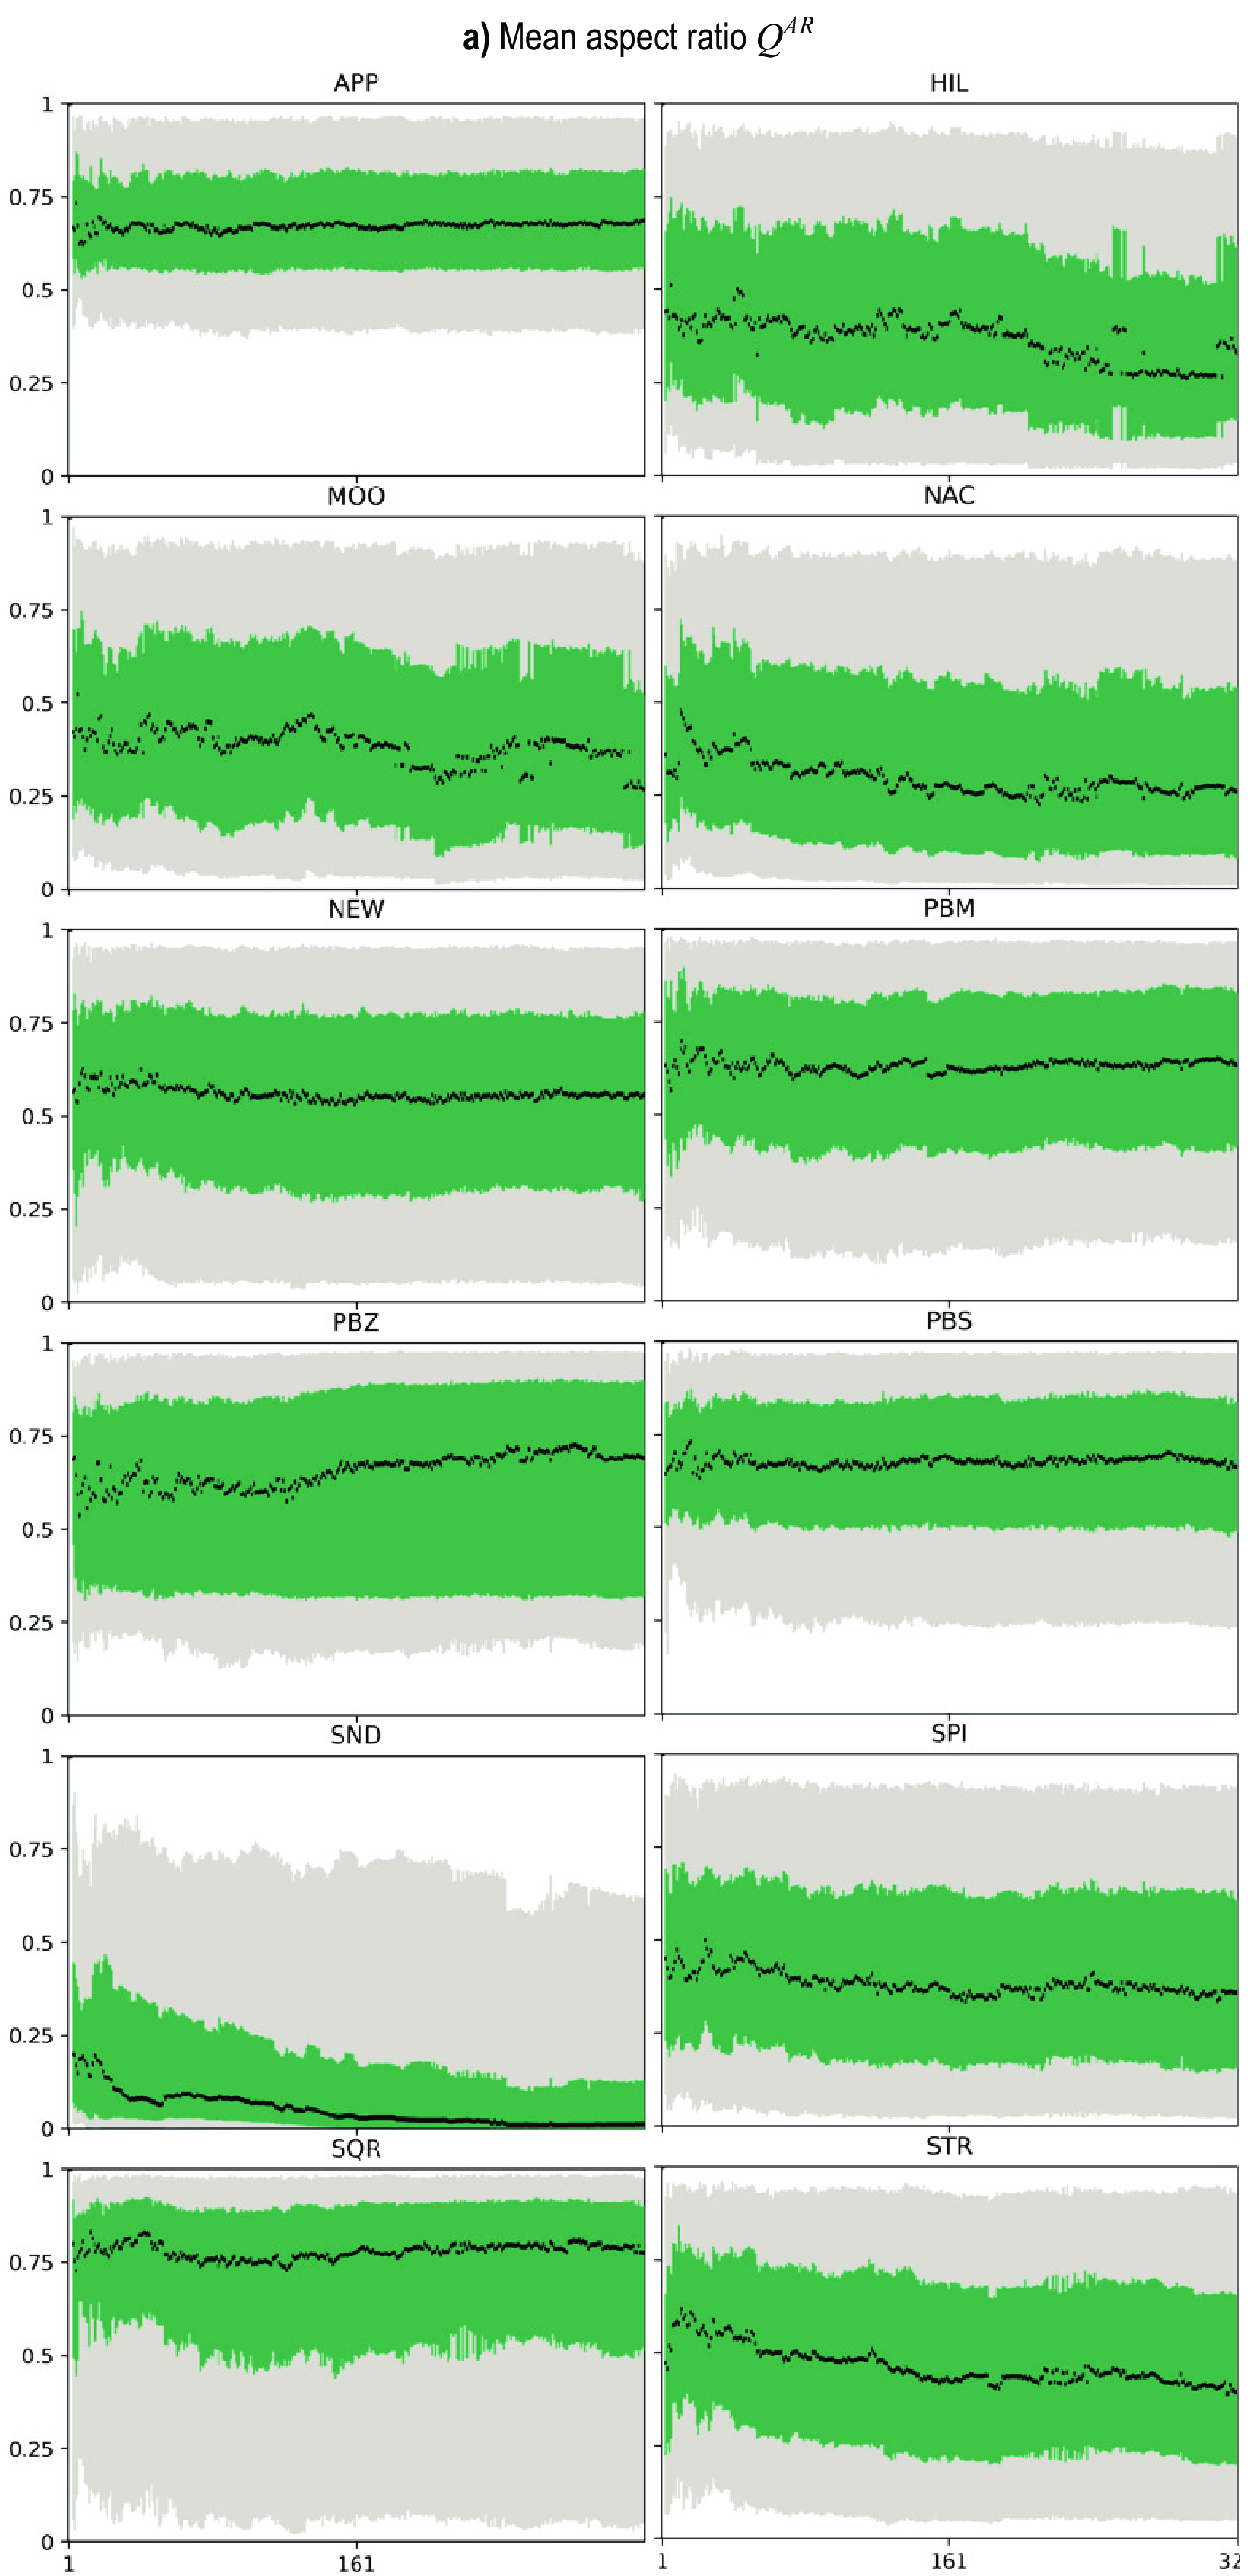
\includegraphics[width=.8\textwidth]{figures/initial-treemap-evaluation/boxplot-a.png}
%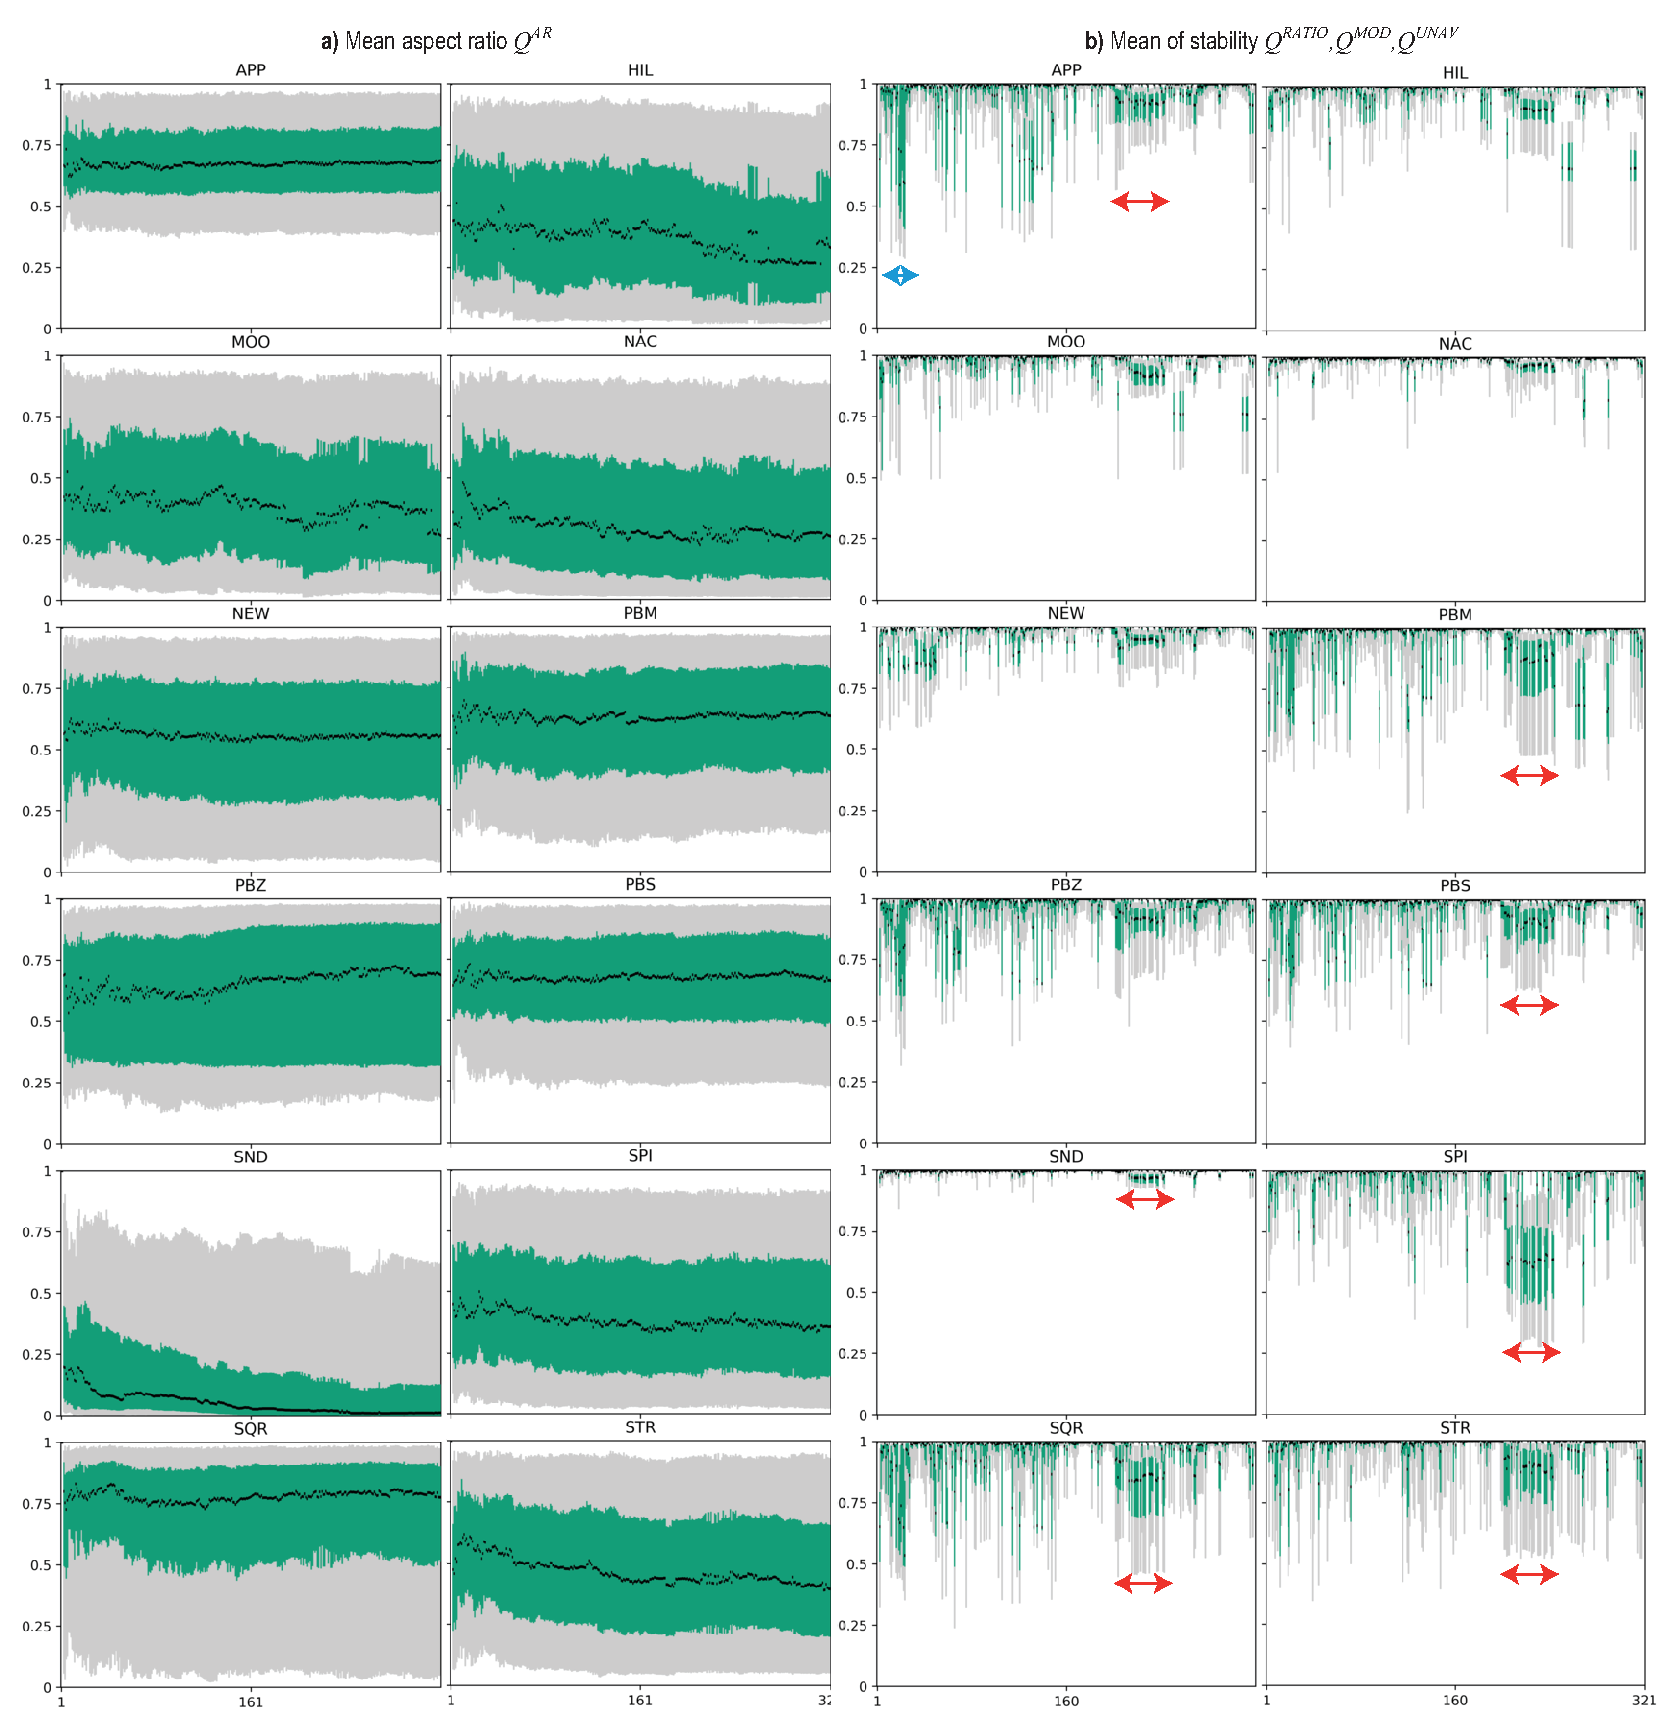
\includegraphics[width=1.0\linewidth]{figures/boxplots.eps}
\vspace{-0.25cm}
\caption{Evolution in time of spatial quality for the \emph{cpython} dataset.}
\label{fig:boxplots_1a}
\end{figure*}

\begin{figure*}[htbp!]
\centering
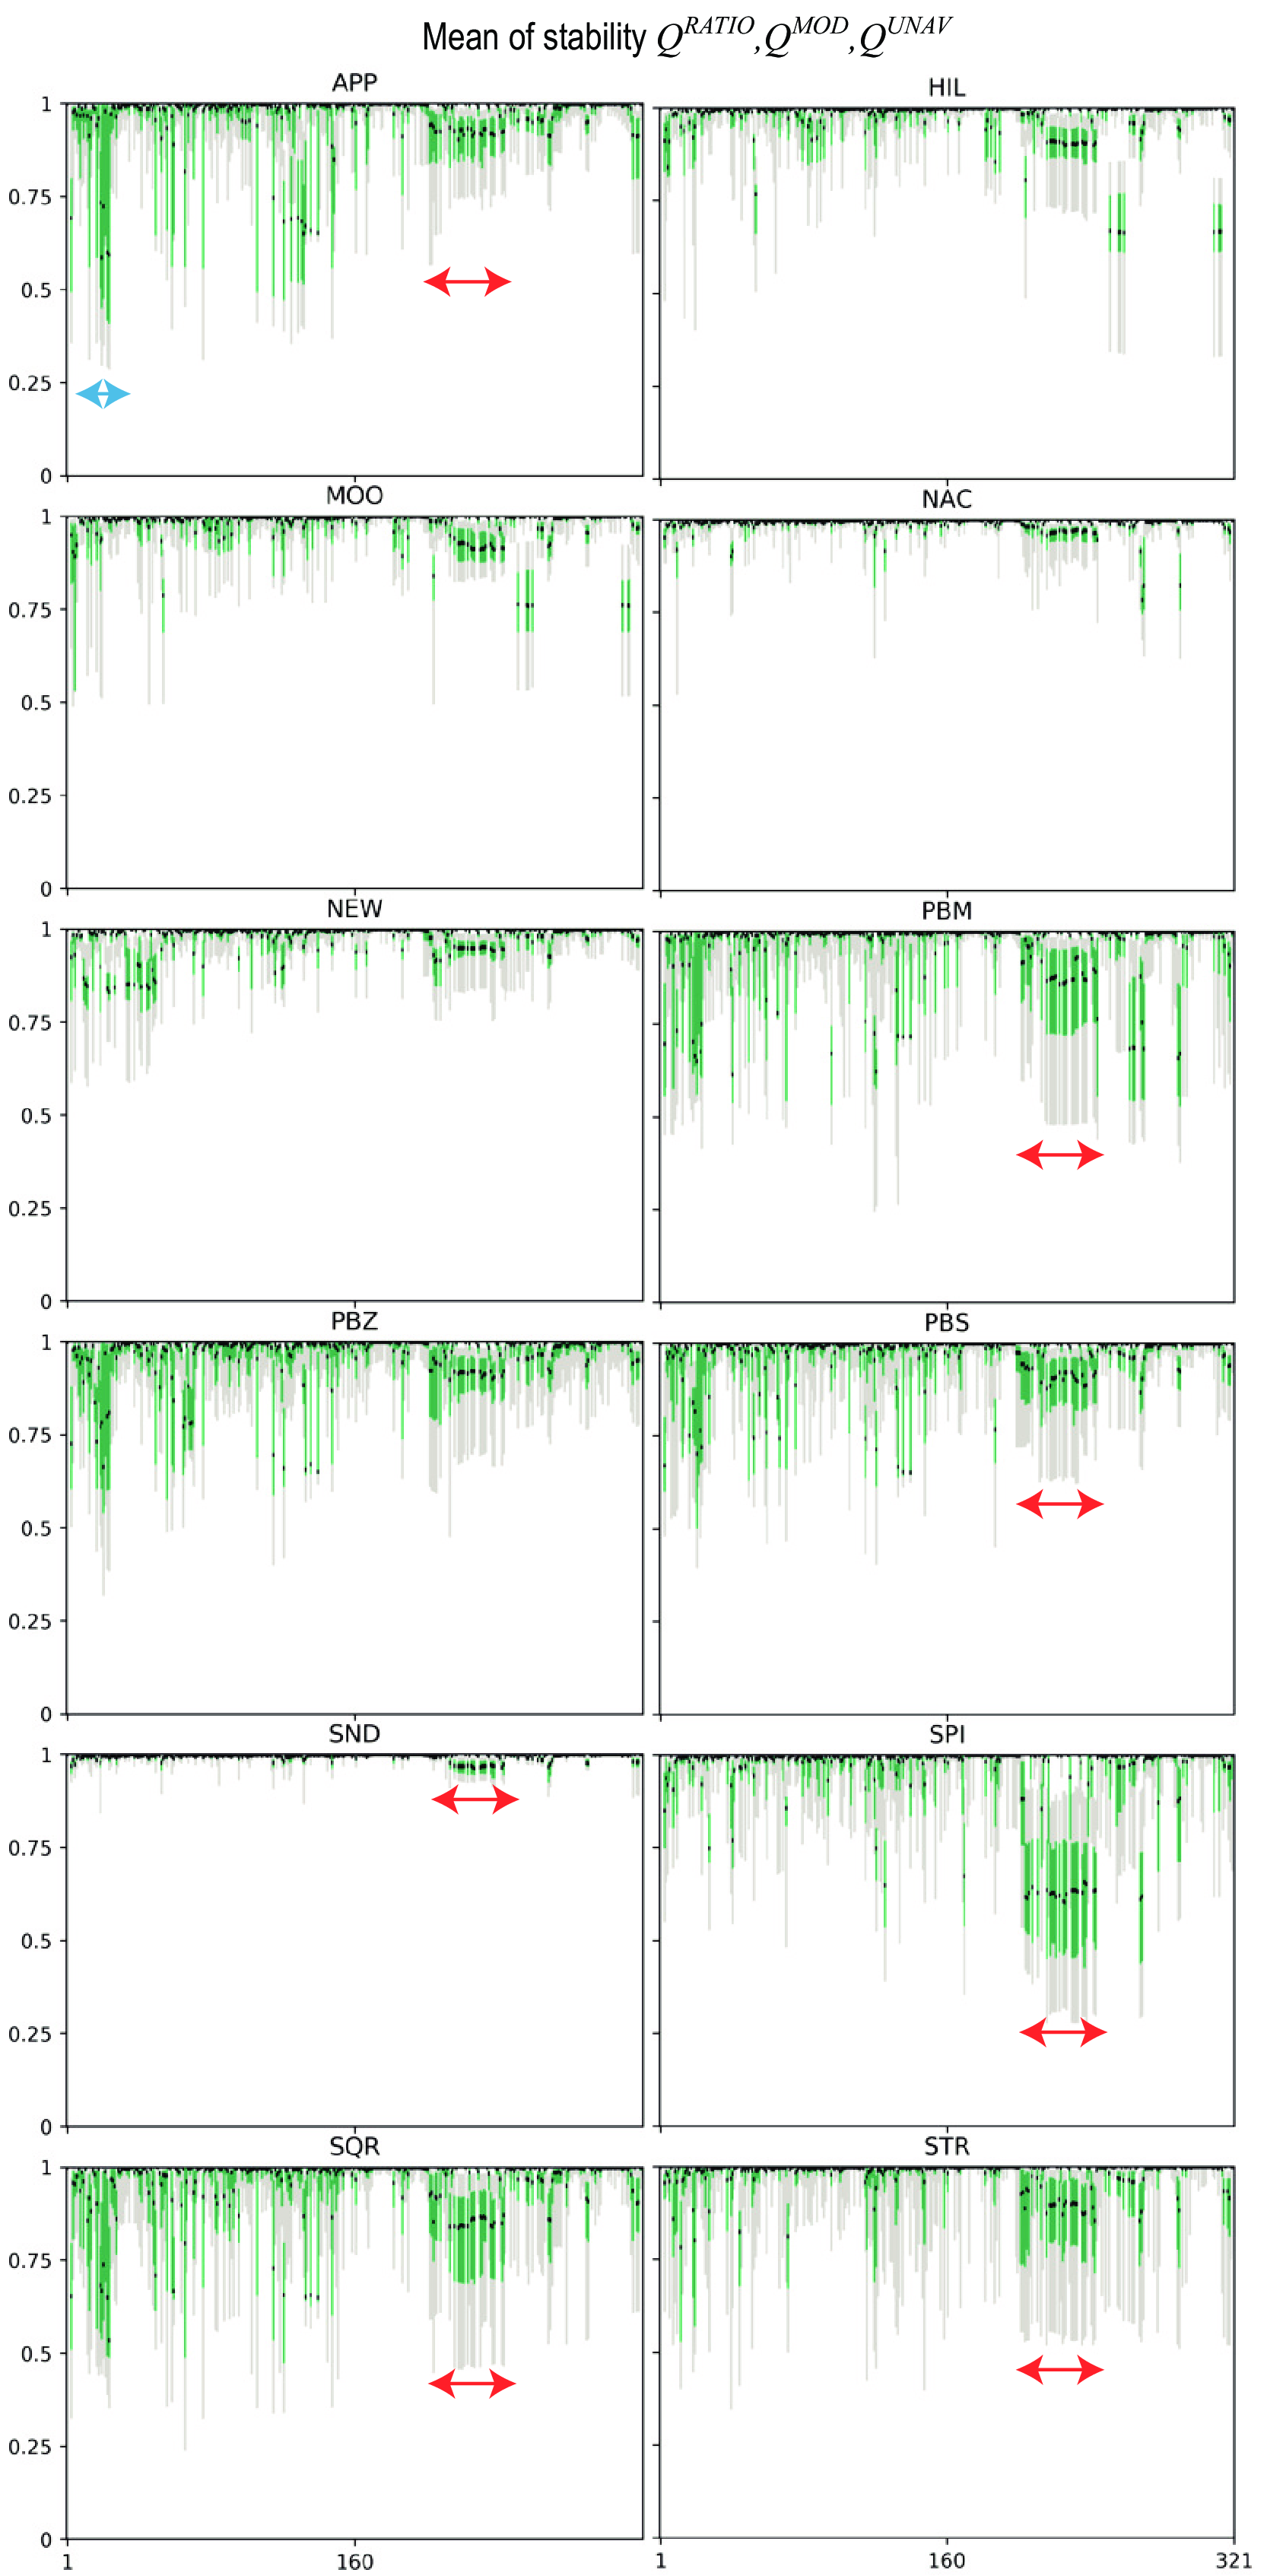
\includegraphics[width=.8\textwidth]{figures/initial-treemap-evaluation/boxplot-b.png}
%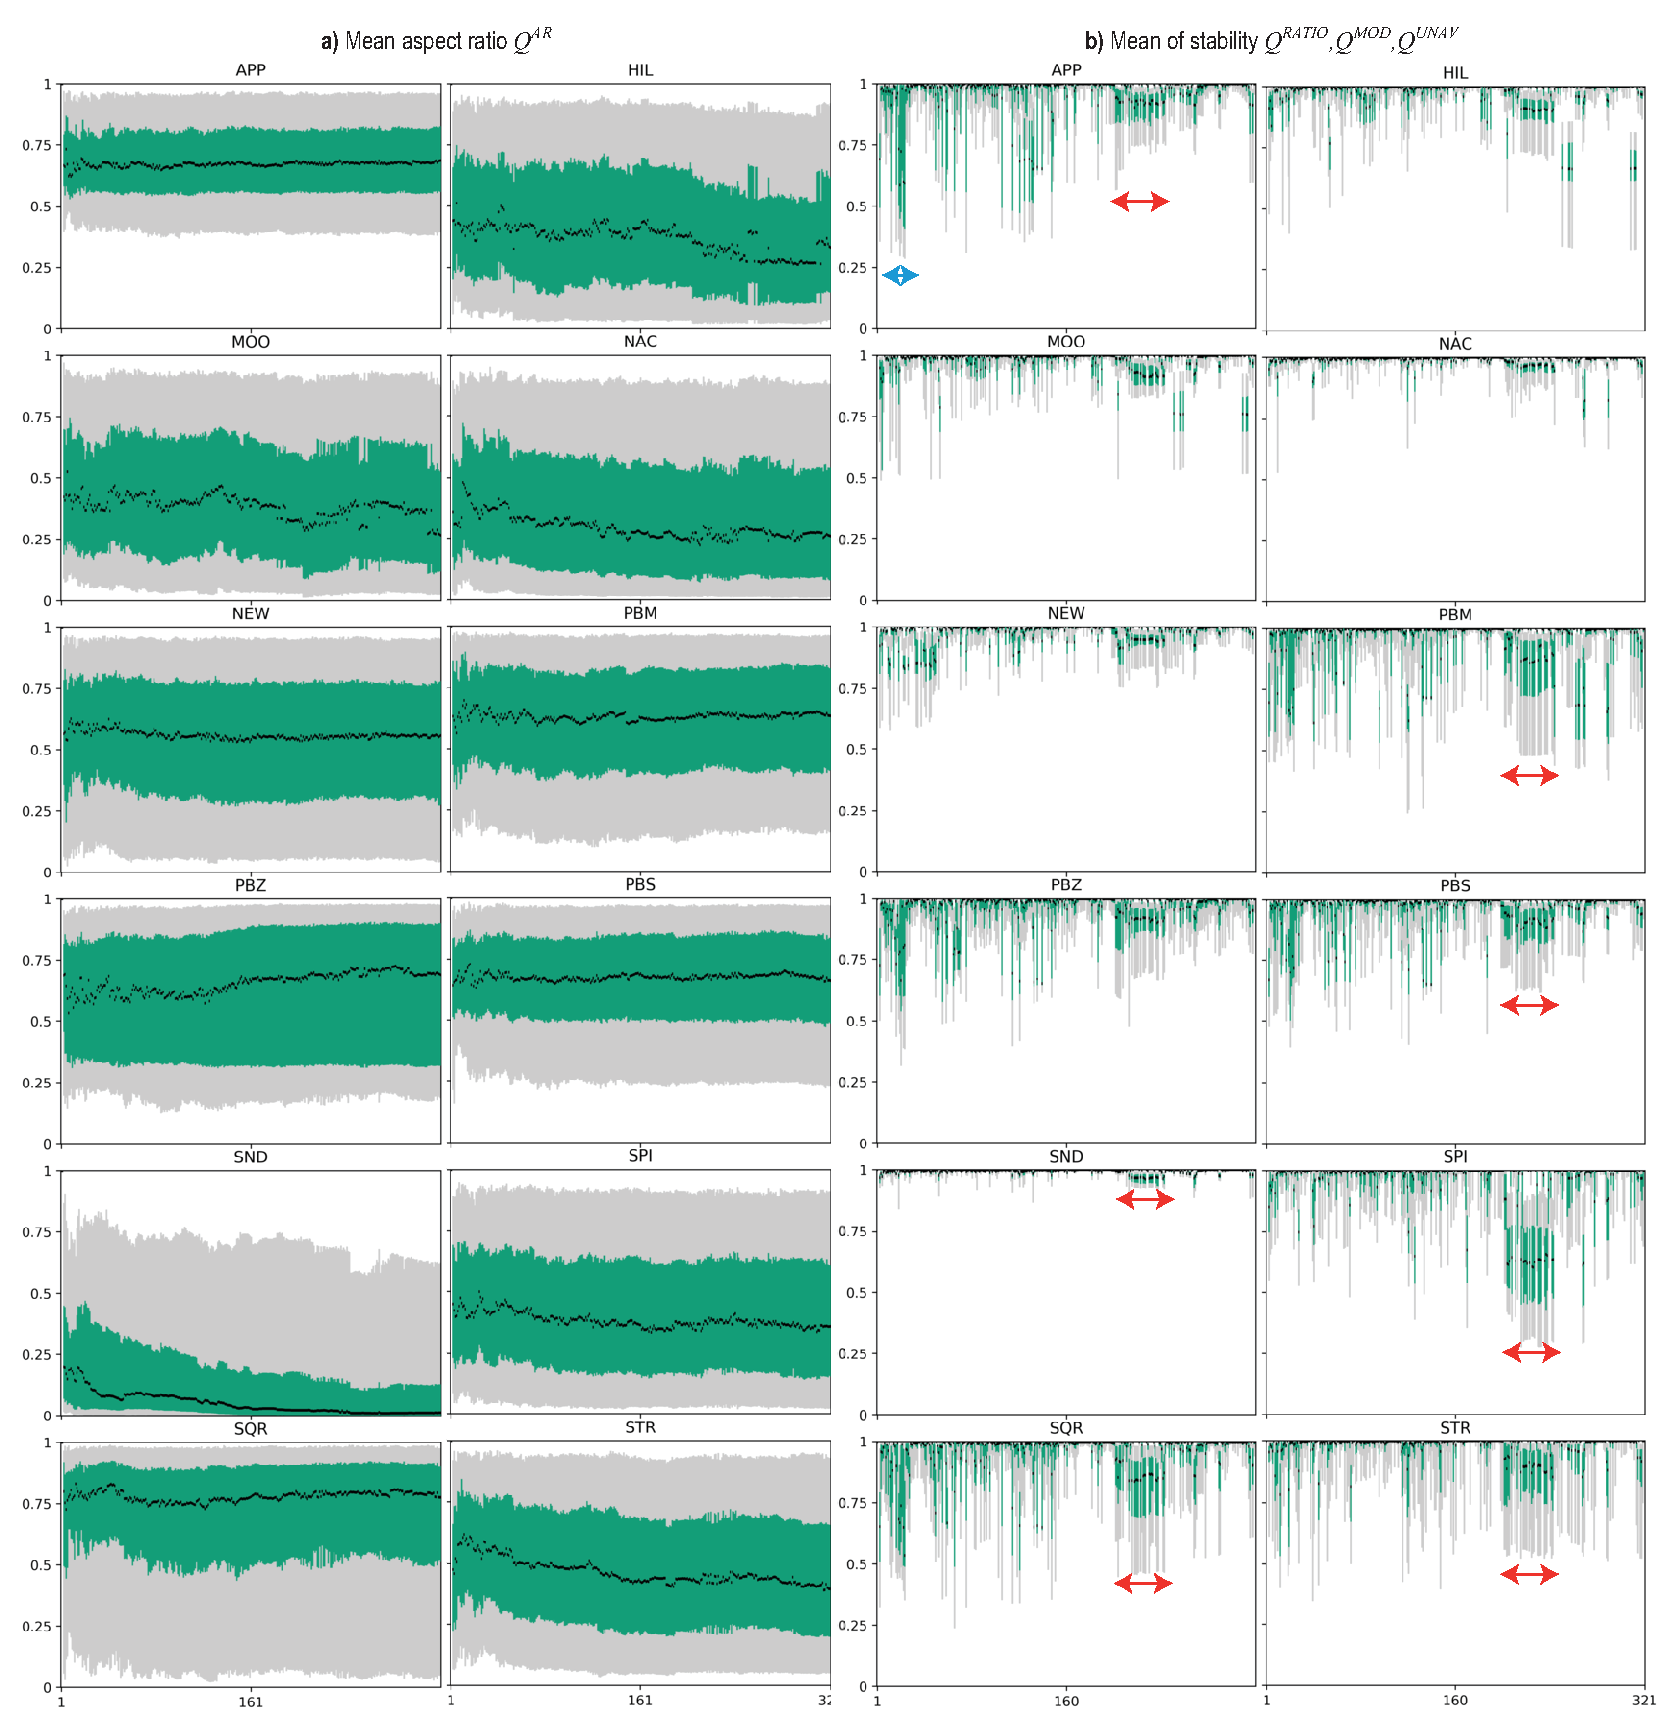
\includegraphics[width=1.0\linewidth]{figures/boxplots.eps}
\vspace{-0.25cm}
\caption{Evolution in time of the averaged four stability metrics for the \emph{cpython} dataset.}
\label{fig:boxplots_1b}
\end{figure*}

Figure~\ref{fig:boxplots_1a}a shows the evolution of the $Q^{AR}$ metric (Eqn.~\ref{eqn:spatial_ratio}) for all tested methods for \emph{cpython}. We see that APP and PBS deliver overall quite high and constant-over-time aspect ratios (0.7), so they are the best methods for spatial quality, with APP being better as it has a narrower $Q^{AR}$ spread around a slightly higher median value. SQR scores higher median values, but has a larger spread -- for every revision, it can score as bad as 0.05 aspect-ratio, while APP does not drop below 0.4 (compare the bottoms of the gray bands in Fig.~\ref{fig:boxplots_1a} for APP and SQR). SND shows the worst spatial quality, with a tight spread around a median $Q^{AR}$ below 0.1. The chart also tells us that most methods deliver \emph{consistent} spatial quality regardless of the data changes in the 321 revisions (which we found to be large by manually examining the sequence). The quality decrease shown by SND and (less) by HIL and STR is somehow surprising, as none of the studied methods uses a `history' of the tree-sequence in its layout heuristics.

Figure~\ref{fig:boxplots_1b}b shows the evolution of four stability metrics $Q^{RATIO}$, $Q^{MOD}$, and $Q^{UNAV}$, averaged per time-step. Compared to spatial quality, we see now much more variation between methods and also much more variation (of the stability) over time. We see that SND is by far the most stable method, whereas SQR, SPI, and PBM score worst. Long `icicle' like boxplots indicate revisions where much more visual change was present than `warranted' by the data change. Interestingly, these appear at the same moments for different algorithms (Fig.~\ref{fig:boxplots_1b}b, red markers shows one example). For such moments we see large variations across methods: For SPI, this is the most unstable part of the sequence, both in median and 5-95\% range sense, whereas APP finds earlier sequences (marked in blue in Fig.~\ref{fig:boxplots_1b}) which are harder to lay out stably.

%
% Refinements:\\
%
% Aggregate all the metrics in the same family (AR and STAB) when you generate every single plot (so, for one dataset, we will have M*2 plots, two plots (AR and STAB) for every of the M methods).
% We also cannot have 30*M*2 plots in the paper. So, select 1..max 2 interesting datasets, like, the largest ones, to generate these plots (so we have in total either 2*M or 4*M individual plots).
% make sure, when you generate the plots, that you use the most up-to-date definitions of AR and STAB metrics! We used some pretty old/early versions of these in the snapshot above.


\subsection{How do methods perform on different datasets (Q3)?}
\label{sec:q3}
%
%
So far, we presented charts that aggregate over all datasets (Sec.~\ref{sec:q1}) or focus on a single dataset, but aggregate all stability metrics (Sec.~\ref{sec:q2}). We would like to see how the proposed stability metrics compare to each other, as we are still in the process of understanding their measurement characteristics. Also, we would like to see how these metrics vary over several datasets. For these goals, we use a set of table views, one per quality metric. In each table, columns are datasets and rows are algorithms. Each cell thus encodes the average value of one quality metric for one dataset tested by one algorithm. Cells are colored with a luminance-based colormap, with data values separately normalized per metric table, so that darkest cells indicate worst cases in all tables (but with potentially different metric absolute values), and brightest cells indicate best cases in all tables.

\begin{figure}[htbp!]
\centering
  \includegraphics[width=.8\linewidth]{figures/initial-treemap-evaluation/matrixplots.eps}
\vspace{-0.1cm}
    \caption{The five quality metrics for all tested methods, all datasets.}
\vspace{-0.2cm}
  \label{fig:table}
\end{figure}

Figure~\ref{fig:table} tells several interesting things. Scanning the first table row-wise, we see that there are no large aspect-ratio quality differences between the tested datasets. This says that most methods (with the notable exception of SND) achieve quite good aspect ratios for a wide dataset variation. Over all datasets, APP is the best method, surpassed by SQR only for a few datasets. Conversely, we see that SND is the most stable method with respect to all four considered stability metrics. Stability-wise, we see that some datasets (\emph{hospitalrun-frontend}, \emph{Leaflet}, and \emph{PhysicsJS}) consistently score worse than all others for basically all algorithms. These are also the datasets yielding the worst stabilities, when PBM, SQR, STR, and SPI methods are used. This indicates that these methods are quite sensitive in stability on the type of input dataset so, for obtaining higher stabilities, other methods should be used. At a higher level, we see that the $Q^{RATIO}$, $Q^{MOD}$, and $Q^{UNAV}$ stability metrics yield very similar plots. This is an interesting finding, since the metrics have quite different formulations (Sec.~\ref{sec:init_metrics}), and indicates that the results can be trusted -- the chance of three metrics having such different expressions yielding so similar values being very small. In contrast, the $Q^{CORR}$ metric has much lower values, which is explained by the fact it is much more conservative -- a good algorithm would need to yield very well correlated $\delta a_k$ and $\delta c_k$ values, and we have seen in Sec.~\ref{sec:q1} that this is by far not the case. We conclude that visual \emph{vs} data change correlation is a too strong quality desiderate for dynamic treemaps handing large real-world datasets, and advise next to use in practice any of the $Q^{RATIO}$, $Q^{MOD}$, and $Q^{UNAV}$ metrics to gauge stability, or, as we have done in Sec.~\ref{sec:q3}, their average value.

\begin{figure*}[htbp!]
\centering
%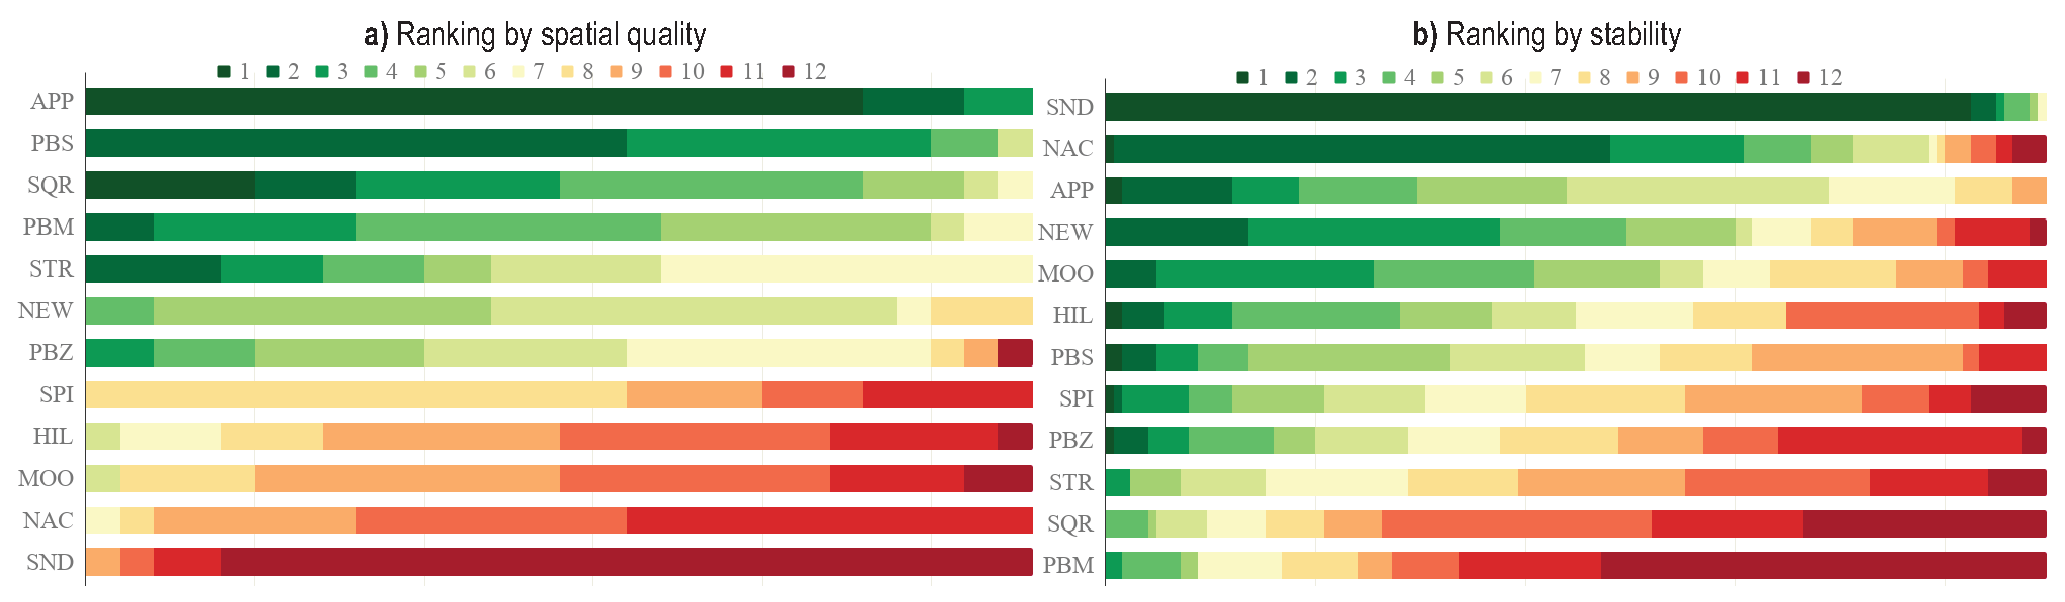
\includegraphics[width=.8\textwidth]{figures/rankcharts.eps}
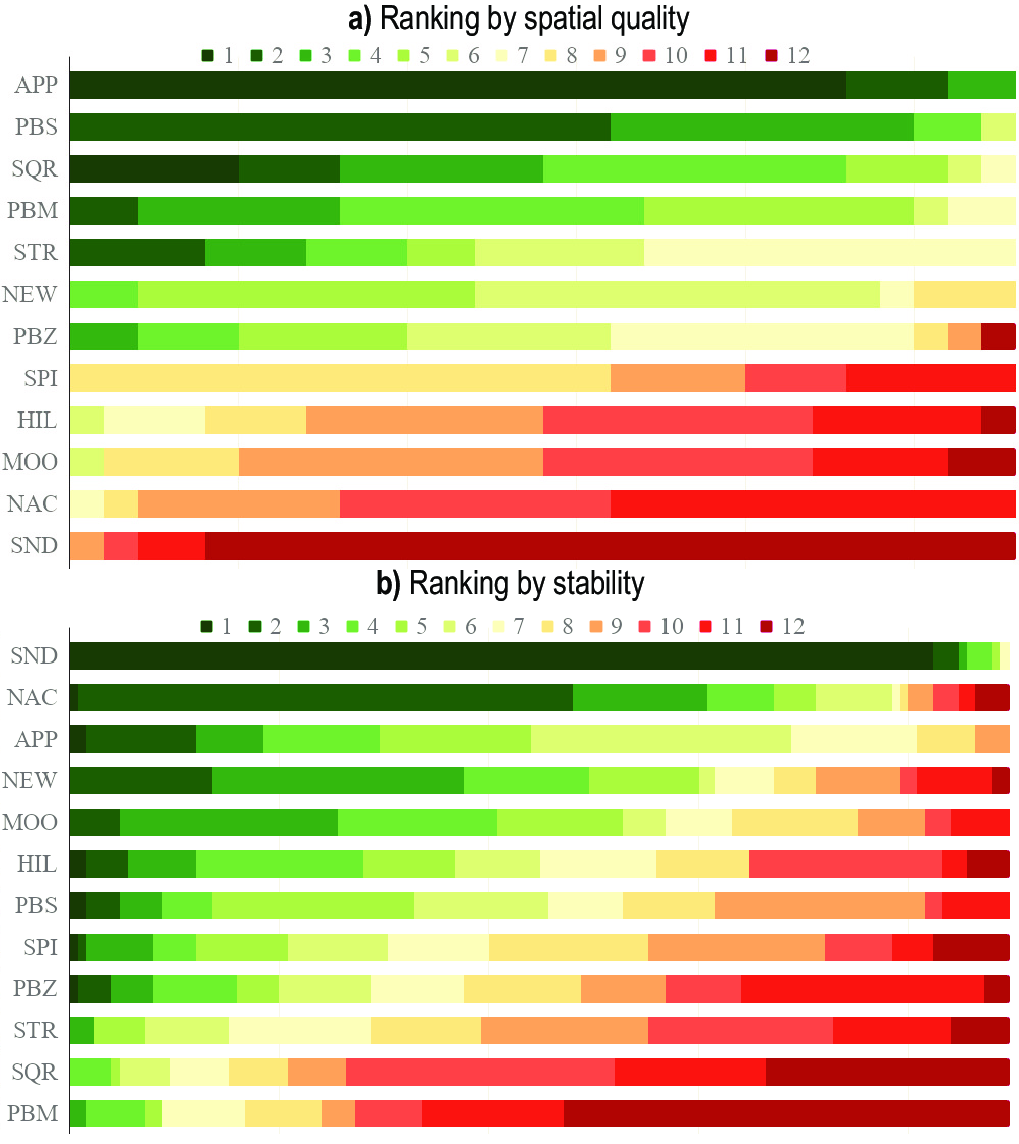
\includegraphics[width=0.9\textwidth]{figures/initial-treemap-evaluation/rank-vertical.png}
\vspace{-0.1cm}
\caption{Ranking of the 12 methods showing the percentage of times they scored a certain rank with respect to spatial quality (a) and averaged stability (b).}
\vspace{-0.2cm}
\label{fig:rankchart}
\end{figure*}

\subsection{How to summarize the comparison (Q4)?}
\label{sec:q4}
%
%
The visualizations so far (Q1--Q3) have given us several insights: We have seen that APP, PBS, and SQR are the best methods with respect to spatial quality, while SND performs poorly for that, but it is the best for stability; different methods have quite different spreads of quality over a given tree sequence, some delivering more consistent results than others, but for most algorithms do not degrade over time; and several of the proposed stability metrics are strongly correlated. It is now useful to \emph{summarize} our findings to present a compact ranking of the tested methods. For this, we use two stacked bar charts. Each bar maps one method and is divided into segments. A segment's length tells the percent of the total number of versions (of all datasets) for which that method had a specific rank regarding spatial quality (Fig.~\ref{fig:rankchart}a) and averaged stability metrics (Fig.~\ref{fig:rankchart}b). We color segments by an ordinal colormap to show these ranks (1 being the best and 12 being the worst). Bars (methods) are sorted in each chart to put the one with highest average rank, weighted by the percents of the total number of versions for all obtained ranks, at the top (Fig.~\ref{fig:rankchart}). From Fig.~\ref{fig:rankchart}, we first see that spatial quality and stability are strongly inversely correlated -- methods that score well on one tend to score poorly on the other. We also see that the top methods in both charts are very good for \emph{most} of the tested datasets, \emph{i.e.}, it is easy to find a method that optimizes either spatial quality or stability, but not both. Interestingly, APP (a less known method) is better in spatial quality, and significantly better in stability, than SQR (arguably the method of choice for creating good aspect-ratio treemaps), so it should be preferred to SQR. Similarly, for stability, APP and NEW (two less known methods) are in the top-four most stable methods, and while worse than SND (very well known method), they have higher spatial quality, so they should be preferred to SND.

\begin{figure}[htbp!]
\centering
%\includegraphics[width=.4\textwidth]{figures/starplot.eps}
\includegraphics[width=.85\linewidth]{figures/initial-treemap-evaluation/starplot.eps}
\vspace{-0.1cm}
\caption{Summarized comparison of all methods (colored dots) on all datasets (colored lines) \emph{vs} spatial quality and stability.}
\vspace{-0.2cm}
\label{fig:starplot}
\end{figure}

A disadvantage of the rank charts in Fig.~\ref{fig:rankchart} is that they do not easily allow linking spatial quality and stability. To alleviate this, we propose a final visualization which uses a start plot metaphor (Fig.~\ref{fig:starplot}). The scatterplot points (circles, categorically colored) are methods attributed by their average spatial quality and stability over all datasets, all revisions. Each method is linked with the 28 tested datasets by same-color lines; a line's endpoint has the average spatial quality and stability over all its revisions for the corresponding method. The plot conveys several insights: First, methods follow roughly a concave curve (Fig.~\ref{fig:starplot}, thick dashed curve), telling the trade-off between spatial quality and stability. Variation in average spatial quality is much larger (roughly 45\%) than in average stability (roughly 8\%). The fan-out of lines from a method shows how predictable that method is, and here we see large variation over methods, with \emph{e.g.} APP being quite consistent in spatial quality, while MOO, STR, and SND show large dataset-dependent variations in both spatial quality and stability (see Fig.~\ref{fig:starplot}, thin dashed curves). The latter is especially interesting: Even though SND has the highest average stability, it can also score worse than many other methods on certain datasets.

To conclude, it is hard to designate an `optimal' method, as this strongly depends on which of stability and spatial quality users see as most important for their concrete use-cases, and by how much. Still, based on all our insights, we believe that APP offers a very good compromise -- very high spatial quality and overall stability similar to most methods, surpassed only (and not in all cases) by SND.


\section{Discussion}
\label{sec:init-discussion}
%
%
Let us discuss our results in the light of the dimensions of evaluating treemap algorithms for software evolution visualization (Sec.~\ref{sec:current_state}):\\

\noindent\textbf{Algorithms:} We consider 12 well-known treemap methods, in contrast to typically 2--3 techniques in current treemap evaluations in software visualization papers. We argue that this gives valuable insights on the suitability of such well-known methods for handling evolving software trees, so it makes the choice of a given method easier for the software visualization practitioner. For instance, our evaluation can tell the interested user which are the advantages (or limitations) of a \emph{given} algorithm \emph{vs} another given algorithm, from the perspectives of spatial quality or stability.\\

\noindent\textbf{Datasets:} Our treemap benchmark cannot cover all variations of trees extracted from software evolution use-cases. However, it measures in total roughly $1.9 \cdot 10^{9}$ treemap cells for 28 tree sequences up to 321 time-steps (revisions). The size and variability of tree sequences covered by our study is larger than all existing similar evaluations of dynamic treemaps in software visualization. However, we admit that we cannot \emph{extrapolate} from this evaluation to draw statistically strong conclusions concerning the quality of a given treemap algorithm for the \emph{entire} space of evolving software hierarchies. Doing so would require (a) a characterization of this space in terms of objective metrics (\emph{e.g.}, tree size, depth, type of structure, type of changes); (b) a targeted search of software repositories to extract trees which `sample' well all these dimensions; (c) an evaluation of our metrics on this benchmark; and (d) most importantly, finding possible correlations between the measured performance of algorithms and the characteristics of the tree sequences they work on. We acknowledge these limitations, and outline them as important directions for future work.\\

\noindent\textbf{Metrics:} We measure treemap stability by essentially considering the first derivative of the treemap algorithm function mapping from tree-node weights to rectangular cell-sets. We detail four variants for measuring stability this way, and observe that three of them, while quite different in terms of actual definitions, yield very similar results. We believe this is an important finding, as it motivates the idea of defining stability by relating visual change to data change. The fourth stability metric (Pearson correlation) showed however to be of limited practical use, as typical dynamic treemaps exhibit a too low correlation of the data and visual changes as compared to other phenomena where this metric is used. This can also indicate that dynamic treemaps may exhibit a more \emph{complex} form of data \emph{vs} visual change correlation than a \emph{linear} one. 
Concluding, we argue that measuring stability by involving both visual and data change is desirable, but we acknowledge that more work is needed to further refine the definition of the proposed stability metric, so that it avoids potential normalization biases, and it also captures in a more demonstrable way what actual users perceive as `unstable'.\\

\noindent\textbf{Result exploration:} We present five visualizations of treemap quality metrics, covering all involved dimensions: cells, revisions, datasets, metrics, and algorithms. As the dimensionality of this data space is large, we obviously cannot cover \emph{all} possible viewpoints. Yet, our visualizations help finding novel insights on the behavior of dynamic treemaps for evolving software hierarchies, and also confirm earlier observations, \emph{e.g.} the known stability of SND. Our visualizations can be used to both analyze fine-grained details (at cell level) and present aggregated conclusions (at algorithm level). They can help the practitioner in understanding what is gained, and/or lost, by choosing a certain treemap algorithm instead of another one.\\

\noindent\textbf{Replicability:} All our results (datasets, treemap and visualization code, measurements) are available online at~\citep{benchmark}. To our knowledge, this is the first benchmark for (dynamic) treemaps for applications in software evolution understanding. It can serve both for practitioners interested in choosing an algorithm based on specific quality criteria, but also for researchers aiming to benchmark their new algorithms, with limited effort, against existing ones.\\

\noindent\textbf{Limitations:} There are several points which can be covered better. First and foremost, as mentioned, we need a more principled sampling of the space of trees extracted from software evolution to gain more confidence in the obtained quality results (or how these would differ as a function of the tree sequences' characteristics). We argue that our current work, \emph{i.e.} the \emph{automated} set-up of the extraction pipeline of dynamic trees from software repositories, computation of the proposed quality metrics, and visualizations that aggregate these, forms the necessary basis for such extensions, which we consider as future work. Separately, more treemap algorithms could be considered, \emph{e.g.}, Voronoi, hybrid, or bubble ones. This will require an adaptation of the spatial quality and stability metrics so they can be used for non-rectangular cells.\\

\noindent\textbf{Threats to validity:} Similar to software quality, we measure treemap quality by a number of `proxy' metrics. While we argue for these metrics at technical level (see the stability metric \emph{vs} function continuity discussion) or, separately, reuse well-known metrics (see the aspect-ratio metric), we do not have hard evidence that such metrics truly capture quality as seen by the eyes of the beholder (end user). The advantage of using such `intrinsic' quality metrics is that they can be computed automatically, on a large benchmark, and are independent on actual tasks, users, or use-cases. This allows for direct and objective comparisons, parallel to what is done on the context of \emph{e.g.}  Graph Drawing \citep{hachul,battista}, where metrics such as number of crossings, angle of crossings, and distribution of edge lengths are used to rank the quality of graph drawing algorithms. 
The disadvantage is that we cannot directly infer, from such metrics, how fit to purpose a given treemap technique will be given a specific user, use-case, type of dataset, and task. We argue for our approach as follows: \emph{if} for a given user, use-case, and task, one agrees that a good treemap algorithm should have the properties captured by our quality metrics, \emph{then} one can use our evaluation and related artifacts (benchmark, metrics, visualizations) to find the best suitable algorithms.


\section{Conclusions}
\label{sec:conclusions}
%
We have presented an evaluation of treemap algorithms for the visualizaton of dynamic tree sequences extracted from the evolution of software repositories. For this, we proposed a benchmark formed by 28 datasets extracted from well-known software repositories, five metrics that aim to capture spatial quality and stability, and 12 known treemap methods. We also propose six visualizations aimed at interpreting the measurement results from several angles, covered by four types of questions. All results (datasets, treemap implementations, measurement code, and visualizations) are publicly available and can constitute the basis of a benchmark for treemap evaluation for visualizing evolving software hierarchies. 

Several directions exist for extending this work. First and foremost, a finer-grained analysis of the space of evolving software trees can be made to elicit correlations between characteristics of the datasets and measured quality of the tested treemap methods. Secondly, and at a higher level, it would be useful to extend this type of benchmarking to other application domains that generate dynamic trees and use treemap methods to visualize their evolution in time. This second direction of work will be further explored in the next chapter.


\chapter{Generalized Treemap Evaluation}
\blfootnote{This chapter is based on the paper ``Quantitative Comparison of Time-Dependent Treemaps'' \citep{vernier_treemap}}
\label{ch:tree-eval}

\newcommand{\mypar}[1]{\smallskip\noindent{\bfseries #1.}}


% The Eurovis 2020 paper with Betina's group is hosted at 
% https://www.overleaf.com/project/5b72c3461a742c3da836ed6b

% What’s the big diff in Ch 3 vs Ch 2? That we now use a far wider set of dataset types, and we think on how to sample the ‘space’ of timedep hierarchies. We’re not looking only at hierarchies from software, but many more. So, this chapter extends the approach, evaluation, etc from Ch 2 to simply a larger space of datasets. Again, make sure you make this clear in the abstract.

\textit{
In the previous chapter, we have presented an evaluation of 12 algorithms designed for construction of static treemaps for the visualization of dynamic hierarchies. 
The evaluation has outlined that there is no ideal treemapping algorithm that optimally balances stability against visual quality. While these results 
indicate that better treemapping algorithms could be designed for the visualization of dynamic hierarchies obtained from evolving software systems, an important question is whether we can extrapolate
these findings to dynamic hierarchies that emerge from datasets coming from different domains. Additionally, there are more treemapping algorithms, and more ways to gauge their quality, than those 
which have been considered in the previous chapter. In this chapter, we extend the evaluation from the previous chapter to cover the above directions. First and foremost, we consider dynamic hierarchies produced by a wide range of application domains, and, to
address this aspect, we propose a strategy to comprehensively sample the space of time-dependent hierarchical datasets. Secondly, we consider additional quality metrics and ways to compare the performance of the studied algorithms. Finally, we consider a few recent treemapping algorithms that were not used in the evaluation in the previous chapter. Taking all these aspects together, the work presented in this chapter represents the most comprehensive quantitative evaluation of dynamic treemaps presented in the literature.
}

\vspace{5mm} %5mm vertical space


\noindent \textbf{Abstract:}
Rectangular treemaps are often the method of choice to visualize large hierarchical datasets. Nowadays such datasets are available over time, hence there is a need for (a) treemaps that can handle time-dependent data, and (b) corresponding quality criteria that cover both a treemap's visual quality and its stability over time.
%
In recent years a wide variety of (stable) treemapping algorithms has been proposed, with various advantages and limitations. 
We aim to provide insights to researchers and practitioners to allow them to make an informed choice when selecting a treemapping algorithm for specific applications and data. To this end, we perform an extensive quantitative evaluation of rectangular treemaps for time-dependent data.
%
As part of this evaluation we propose a novel classification scheme for time-dependent datasets. Specifically, we observe that the performance of treemapping algorithms depends on the characteristics of the datasets used. We identify four potential representative features that characterize time-dependent hierarchical datasets and classify all datasets used in our experiments accordingly. We experimentally test the validity of this classification on more than 2000 datasets, and analyze the relative performance of 14 state-of-the-art rectangular treemapping algorithms across varying features. Finally, we visually summarize our results with respect to both visual quality and stability to aid users in making an informed choice among treemapping algorithms.
All datasets, metrics, and algorithms are openly available to facilitate reuse and further comparative studies.

\section{Introduction}
\label{sec:introduction}

Treemaps are one of the best-known methods for visualizing large hierarchical datasets. Given an input tree whose leaves have several attributes, treemaps recursively partition a 2D spatial region into cells whose visual attributes (area, color, shading, or annotation) encode the tree's data attributes. Compared to other methods such as node-link techniques, treemaps effectively use all available screen pixels to show data, and thus can display trees of tens of thousands of nodes on a single screen. Most treemaps use rectangles, although there are alternative models such as Voronoi treemaps~\citep{balzer05b}, orthoconvex and L-shaped treemaps~\citep{deberg14}, and Jigsaw treemaps~\citep{jigsaw}. 
In this paper, we focus exclusively on rectangular treemaps.

The input for a rectangular treemap is a rectangle $R$ and a set of non-negative values $a_1, \ldots, a_n$ together with a hierarchy on these values (represented by a tree). The output is a treemap $T$, which is a recursive partition of $R$ into a set $\mathcal{R}=\{R_1, \ldots, R_n \}$ of interior-disjoint rectangles, where $(a)$ each rectangle $R_i$ has area $a_i$, and $(b)$ the regions of the children of an interior node of the hierarchy form a rectangle (associated with their parent). Such a partition of a rectangle into a set of disjoint rectangles is also called a \emph{rectangular layout}, or \emph{layout} for short. Typically the input values are \emph{normalized}, that is, the sum $A = \sum_i a_i$ corresponds to the area of $R$.

Nowadays, large hierarchical datasets are also available over time. Hence, there is a need for \emph{time-dependent} treemaps which display changing trees and data values. Ideally, such time-dependent treemaps enable the user to easily follow structural changes in the tree and in the data. In a time-dependent setting, the input values become functions $a_i\colon [0, X] \rightarrow \mathbb{R}_{\geq 0}$ for each $i$, where the discrete domain $[0, X]$ represents the different time steps in the data. We assume that the hierarchy on the values and $R$ are not time-dependent, and that the values $a_i$ are properly normalized for each time step separately. We use the special value $a_i(t) = 0$ to represent that data element $i$ is not present at time $t$; and we speak of insertions or deletions if $a_i(t)$ starts or stops to be nonzero, respectively.

The \emph{visual quality} of rectangular treemaps is usually measured via the aspect ratio of its rectangles. This indicator can become arbitrarily bad: Consider a treemap that consists of only two rectangles. If the area of one of these rectangles tends towards zero, then its aspect ratio tends towards infinity. \cite{nagamochi07} describe an algorithm (APP) which computes, for a given set of values and a hierarchy, a treemap which provably approximates the optimal aspect ratio. \cite{deberg14} prove that minimizing the aspect ratio for rectangular treemaps is strongly NP-complete. ~\cite{Kong2010} propose perceptional guidelines to improve treemap design and \cite{Zhou2017} perform user studies to test the effectiveness of different rectangular treemapping algorithms. Recently \cite{lu2017golden} argue that the optimal aspect ratio for treemaps should, in fact, be the golden ratio. In Section~\ref{sec:algorithms-2}, we describe the state-of-the-art of rectangular treemaps in detail along with the various characteristics of rectangular treemaps.

For time-dependent treemaps, a second quality criterion is \emph{stability}. Ideally, small changes in the data should result only in small changes in the treemap. Such stable behavior ensures that the only changes the user sees are due to the data, and not due to the decisions the algorithm makes.
%
In recent years a few non-rectangular treemaps were specifically developed for time-dependent data. \cite{hahn10} and \cite{hees17} describe stable versions of Voronoi treemaps. \cite{Chen2017} propose a small-multiple metaphor to visualize time-dependent hierarchies. Their algorithm computes a global layout for all time steps simultaneously, but does not handle insertions or deletions. \cite{Scheibel2018} give an algorithm that maps changes in the data onto an initial layout. However, ``treemaps'' of subsequent time steps are not proper rectangular layouts as white space is introduced when resolving overlaps between rectangles.
%
%Finally, Lukasczyk~\emph{et al.}~\citep{lukasczyk2017nested} and K{\"o}pp and Weinkauf~\citep{kopp2019temporal} show how to compute static overviews of the whole evolution of time-dependent hierarchical data sets, while
%Guerra-G{\'o}mez~\emph{et al.}~\citep{StemView} and Card~\emph{et al.}~\citep{TimeTree} present interactive visualization tools.

A different approach to visualizing time-varying hierarchical data is taken by 
\cite{lukasczyk2017nested}, \cite{kopp2019temporal}, and \cite{li19}, who show how to compute static overviews of the entire evolution of the tree. Alternatively, \cite{StemView} and \cite{TimeTree} use interactivity to explore time-varying data. 
For a broader perspective on tree visualizations, \cite{graham10} present a survey of visualizations that compare multiple trees, while \cite{schulz11_treesurvey} and \cite{scheibel20} present, respectively, a survey and a taxonomy for the visualization of a single tree. 
%Finally H.J. Schulz~\citep{treevis} maintains a large collection of tree visualisation methods. EITHER INCLUDE THIS SENTENCE OR SIMILAIR, OR WRITE SOMETHING IN THE RESPONSE TO REVIEWER WHY WE DON'T WANT TO INCLUDE A WEBSITE (GUARANTEE THAT IT WILL BE MAINTAINED IS MY MAIN ISSUE WITH THAT)

%Our contribution differs significantly from these survey works: We focus specifically on time-varying treemap algorithms (many of which are not covered by these earlier works), and propose and measure quality metrics to quantitatively compare their performance.

\mypar{Contribution} Despite their enduring popularity, a comprehensive evaluation of treemaps is currently lacking, even more so for the time-dependent case. Individual papers tend to report on only a few algorithms and evaluate only a few datasets, often without a principled discussion of quality metrics. To provide insights to both researchers and practitioners and to allow them to make an informed choice when selecting a treemap for their specific application and data, we perform an extensive quantitative evaluation of rectangular treemaps for time-dependent data. Our three main contributions are:

\noindent
\textbf{(1)} We introduce a new method to measure the stability of time-dependent treemaps which explicitly considers the input data (Section~\ref{sec:stablity}). An algorithm is stable if small changes in the input data result in small changes in the layout, that is, data change and layout change correlate positively. Previously proposed stability metrics measure only the layout change and conclude that small layout changes are a sign of a stable algorithm. However, to properly measure stability, we also need to capture the data change and then correlate data and layout change. Here, we have to
overcome the difficulty that the data and the layout space are a priori incomparable. We solve this problem by introducing the concept of a \emph{baseline treemap} $T^*$ which represents the minimum amount of change that any time-dependent treemap must incur (given the input data) when moving from treemap $T$ to the next treemap $T'$.

\noindent
\textbf{(2)} We propose a novel classification scheme for time-dependent datasets. Specifically, based on our discussion of the state-of-the-art of treemaps in Section~\ref{sec:algorithms-2}, we observe that the performance of treemaps depends on the characteristics of the datasets used. We identify four potential representative features that characterize time-dependent hierarchical datasets and classify all datasets used in our experiments accordingly. We experimentally test the validity of this classification on 2405 datasets, and analyze the relative performance of 14 state-of-the-art rectangular treemapping algorithms across varying features. Generally we conclude that our proposed features do indeed have predictive value, both with respect to visual quality and stability. We also observe that algorithms that are designed to be stable tend to in fact be more stable across features.

\noindent
\textbf{(3)} We perform a quantitative evaluation of 14 rectangular treemapping algorithms on more than 2000 datasets. We visually summarize our results with respect to both visual quality and stability to aid users in making an informed choice among treemaps. All datasets, metrics, and algorithms are openly available~\citep{URLTreemaps}. Section~\ref{sec:exploration} reports on our experimental results, we conclude in Section~\ref{sec:discussion-2}.

%Studying how hierarchy visualization algorithms perform has a strong history. For example,
%Li \emph{et al.}\,\citep{li19} and Bremm \emph{et al.}\,\citep{bremm11} present comparisons of multiple hierarchies. Schulz \emph{et al.}\,\citep{schulz11_treesurvey} and Graham and Kennedy\,\citep{graham10} present  broad surveys of tree visualization methods. McGuffin and Robert\,\citep{mcguffin10} propose methods to quantify the space efficiency of various tree visualizations. Finally, Scheibel \emph{et al.}\,\citep{scheibel20} proposes a taxonomy of space-partitioning visualization methods for tree data. Our contribution differs significantly from these works: We focus specifically on time-varying reemap algorithms (many of which are not covered by these earlier works), and propose and measure quality metrics to quantitatively compare their performance.

\section{Rectangular Treemaps}
\label{sec:algorithms-2}
We next discuss the most well-known rectangular treemapping algorithms. For a fair comparison during our experiments, we require that treemap rectangles have exactly the correct areas and partition the input rectangle. Algorithms that do not satisfy these requirements are not included in our evaluation. 
%
 Recall that the input for a rectangular treemap is a rectangle $R$ and a set of non-negative values $a_1, \ldots, a_n$ together with a hierarchy on these values (represented by a tree). The children of a node in this hierarchy are given in a particular order in the input. We distinguish two classes of treemaps, which either do or do not use this order. For time-dependent data we also distinguish between state-aware and stateless treemaps. Contrary to stateless treemaps, state-aware treemaps do not compute the treemap separately at a time step, but (can) use the layout of the previous time step to compute a new layout. Most treemaps are stateless; we discuss the state-aware algorithms separately. 

\smallskip\noindent
\textbf{Unordered treemaps} do not (need to) adhere to the input nodes' order when computing the layout. Typically, input weights are sorted to help the algorithm achieve good visual quality. Unordered treemaps in our evaluation include Squarified treemaps (\textbf{SQR})~\citep{sqr} and Approximation treemaps (\textbf{APP})~\citep{nagamochi07}. APP comes with a guaranteed upper bound on the worst-case aspect ratio, while SQR often achieves near-optimal aspect ratios in practice.
%
The visual quality of unordered treemaps is relatively unaffected by high \emph{weight variance}, as reordering weights allows the layout to group similar-size rectangles in the treemap, typically leading to better aspect ratios. Yet, the sorted order of the weights may change rapidly over time, especially if the \emph{weights change} much over time or if the \emph{weight variance} is low. This can negatively affect the stability of the treemaps. 

\smallskip\noindent
\textbf{Ordered treemaps} are required to adhere to the order of nodes as given in the input, which roughly ensures that rectangles close to each other in the input are close to each other in the resulting treemap. This typically improves the stability of treemaps, but may worsen visual quality. We include nine ordered treemaps in our evaluation. The first ordered treemaps~\citep{ordered} include the Pivot-by-Middle (\textbf{PBM}), Pivot-by-Size (\textbf{PBZ}), and Pivot-By-Split (\textbf{PBS}) algorithms. Similar algorithms are the Strip algorithm (\textbf{STR})~\citep{bederson02} and the Split algorithm (\textbf{SPL})~\citep{engdahl}. Other algorithms, like the Spiral algorithm (\textbf{SPI})~\citep{spiral}, and the Hilbert (\textbf{HIL}) and Moore (\textbf{MOO}) algorithms~\citep{hilbert_moore}, lay out rectangles following a space-filling curve. Finally, the very first treemap algorithm (Slice-and-Dice (\textbf{SND})) by \cite{shneiderman92} can also be considered an ordered treemap. While not ordered by design, the resulting (combinatorial) layout depends only on the hierarchy and not on weights. In fact, SND uses the depth in the hierarchy to compute the layout (slicing vertically on even depth and horizontally on odd depth), rather than simply applying the same algorithm recursively. Hence, SND's visual quality strongly depends on the \emph{number of levels} in the input hierarchy. 
%
Typically, laying out large rectangles near small rectangles leads to poor aspect ratios. Hence, the visual quality of ordered treemaps is negatively affected by high \emph{weight variance}. However, ordered treemaps are relatively stable over time compared to unordered treemaps, as order is maintained. Finally, \emph{insertions and deletions} may affect the visual quality and stability of ordered treemaps to varying degrees, depending on how they are handled exactly.

\smallskip\noindent
\textbf{State-aware treemaps}
can use the layout of the previous time step to compute a new layout and so can largely control their stability. 
The treemap for the first time step is typically an existing unordered treemap. 
The first state-aware treemap was introduced by \cite{sondag17}. Their Local Moves algorithm (LM) is initialized with APP, and allows only a small number of local modifications to the (combinatorial) layout between time steps. They also show how to update areas between time steps without significantly changing the layout (layouts remain ``order-equivalent''). In our evaluation we include the Local Moves algorithm with 4 local moves between time steps (\textbf{LM4}), and without local moves (\textbf{LM0}). A similar algorithm is the Git algorithm (\textbf{GIT}) \cite{vernier18git}, which is initialized with SQR, and does not allow any changes to the (combinatorial) layout between time steps. Git is described in full detail in Chapter~\ref{ch:git}, as it is a particular contribution to this thesis.
Both state-aware treemaps also support insertions and deletions, updating the layouts locally where necessary (for insertions, the position in the layout can be chosen to maximize visual quality).
%
By design, the stability of state-aware treemaps is relatively unaffected by frequent \emph{weight changes} over time. Also, the visual quality of the initial treemaps should be relatively high. However, since the layouts cannot change much over time, the visual quality of state-aware treemaps will decrease over time if weights change significantly. Frequent \emph{insertions and deletions} may also cause treemaps with poor visual quality, as treemaps are not recomputed as a whole. However, many insertions can help to correct rectangles with bad aspect ratio caused by weight changes over time. This is especially helpful for state-aware algorithms that do not allow any changes to the layout, like LM0 and GIT. Note that SND has a fixed layout if the input hierarchy does not change and is hence very stable, but it does not explicitly use the previous state.

Finally, note that the \emph{number of levels} in the input hierarchy can have a strong effect on all classes of algorithms. In general, more levels imply less freedom in the layout strategy. As a result, unordered treemaps become more similar to ordered treemaps. Overall, the visual quality tends to decrease and the stability tends to increase. 

\section{Metrics}
\label{sec:metrics-2}
\cite{jigsaw} identifies several desirable properties of treemaps: (1) nicely shaped regions (visual quality), (2) stability with regard to changing leaf values, (3) stability with regard to changing tree structure, and (4) preservation of order information. Regarding Property (3), the tree structure can change in various ways; for example, nodes can merge or split, nodes can change parents, or there are general insertions and deletions. In our experiments we do not make any assumptions on the type of changes to the tree structure, and hence treat them as general insertions and deletions. Furthermore, we do not assume that the order of the values in the data is meaningful in general. Thus, we consider the following two important criteria to evaluate treemaps: \emph{visual quality} and \emph{stability}. We discuss well-established metrics for both below. We also introduce a new method to measure the stability of time-dependent treemaps which captures inherent data changes. We compute metrics for each leaf rectangle separately and then aggregate these values for each algorithm and dataset (see Section~\ref{sec:exploration} and ~\citep{URLTreemaps} for details). Note that we do not compute metrics for non-leaf nodes. 

\subsection{Visual quality}
\label{sec:aspectratio}
The weight information in a treemap is conveyed by the areas of its rectangles. Since areas of rectangles closer to squares are visually easier to estimate than areas of elongated rectangles, visual treemap quality is commonly measured by the aspect ratio of its rectangles. Although it has been proposed that the ratio should be close to the golden ratio~\citep{lu2017golden} instead of the minimum aspect ratio of $1$, it is commonly accepted that strongly elongated rectangles hinder readability of treemaps. We thus aim for the overall goal of making rectangles as square as possible, or similarly, minimizing the number of elongated rectangles. For a rectangle $R_i$ of width $w(R_i)$ and height $h(R_i)$, we define the aspect ratio $\rho(R_i)$ as
%
\begin{equation}
\rho(R_i) = \min(w(R_i), h(R_i)) / \max(w(R_i), h(R_i)).
\label{eqn:rho}
\end{equation}
%
Observe that this definition is the inverse of the usual definition for aspect ratio. Its values range from 0 to 1, where values of $\rho$ close to $0$ are considered ``bad'' and values close to $1$ are considered ``good''. The bounded range allows for easy aggregation. Note that, compared to the usual definition of $1/\rho$, rectangles with larger aspect ratios have a smaller influence on the aggregated score.
%especially when computing the mean visual quality of a treemap.

\subsection{Stability}\label{sec:stablity}
%
Evaluating the stability of a treemap is more involved than evaluating visual quality. Consider treemaps at two consecutive time steps $T(t)$ and $T(t+1)$. Since stability does not \emph{explicitly} depend on the value of $t$, we denote the former and the new treemap by $T$ and $T'$ respectively, to simplify notation. We also denote the rectangle areas in $T$ and $T'$ by $\{a_1, \ldots, a_n\}$ and $\{a'_1, \ldots, a'_n\}$, respectively. For a stable treemapping algorithm, the (visual) difference between $T$ and $T'$ should roughly correspond to the difference between $\{a_1, \ldots, a_n\}$ and $\{a'_1, \ldots, a'_n\}$. Note that the combination of large changes in data values and small changes in the layouts is unlikely since rectangle areas in treemaps must exactly match the data values. Hence, we actually want to measure \emph{instability}, that is, large layout changes that are not caused by large data changes.

Most existing treemap stability metrics consider only the visual change in the treemap's layout $d(T, T')$, usually computed by evaluating the change $\delta(R_i, R'_i)$ for each rectangle separately and aggregating it over all rectangles. \cite{ordered} define $\delta$ as the Euclidean distance between the vectors $(x(R_i), y(R_i), w(R_i), h(R_i))$ and $(x(R'_i), y(R'_i), w(R'_i), h(R'_i))$, where $x$, $y$, $w$, and $h$ are the coordinates of the top-left corner, width, and height of a rectangle, respectively. They then define $d$ as the average over all rectangles. Hahn~\emph{et al.}~\citep{hahn10,hahn2015comparing} simplify this metric by defining $\delta$ as the distance moved by the centroid of a rectangle, again defining $d$ as the average. \cite{hilbert_moore} use the same $\delta$ as~\citep{ordered}, but define $d$ as the variance over all values computed by $\delta$. They also propose a drift metric, which measures how much a rectangle moves away from its average position over a long period. Recently, \cite{Scheibel2018} introduced two new layout change metrics: The \emph{average aspect ratio change} defines $\delta$ as the relative change between the aspect ratios of $R_i$ and $R'_i$, and defines $d$ as the average. The \emph{relative parent change} defines $\delta$ as the relative change of the distance between the center of a rectangle and the center of its parent, again defining $d$ as the average. \cite{Chen2017} propose a metric to quantify the ability of users to track time-dependent data in treemaps, which is closely related to the drift metric~\citep{hilbert_moore}. A different approach measures layout change using pairs of rectangles. \cite{Hahn2017} introduce the \emph{relative direction change}, which, for every pair of rectangles $R_i$ and $R_j$, measures how much the angle from the center of $R_i$ to the center of $R_j$ changes. Finally, \cite{sondag17} proposed the \emph{relative position change}, which, for every rectangle pair $(R_i, R_j)$, measures how much the relative position of $R_i$ with respect to $R_j$ changes. The distance $d$ is then defined as the average over all rectangle pairs. 

Summarizing the above, we distinguish two types of layout change metrics: (1) \emph{absolute} metrics measure how much individual rectangles move/change, and (2) \emph{relative} metrics measure how much positions of pairs of rectangles change relative to each other. For our experiments, we use both an absolute and a relative metric. In particular, as an absolute metric, we use the \emph{corner-travel distance}, which is a well-known metric used in computer vision to quantify change between two shapes using feature points~\citep{tuytelaars07,szeliski10}. In the vision community, it was established already many years ago~\citep{shi1994good,biederman87} that corners are a perceptually useful feature to identify and track.
Besides this perceptual validation, the corner-travel metric lies also within a small bounded factor of the original metric introduced by \cite{ordered}. Specifically, let $w(R)$ and $h(R)$ be the width and height of an input rectangle $R$, respectively. Let $p_i$, $q_i$, $r_i$, and $s_i$ ($p'_i$, $q'_i$, $r'_i$, and $s'_i$) be the positions of the corners of a rectangle $R_i$ ($R'_i$). We define the normalized corner-travel (CT) distance for a rectangle as
%
\begin{equation}
\delta_{\text{CT}}(R_i, R'_i) = \frac{\|p_i - p'_i\|_1 + \|q_i - q'_i\|_1 + \|r_i - r'_i\|_1 + \|s_i - s'_i\|_1}{4 \sqrt{w(R)^2 + h(R)^2}}.
\label{eqn:delta_ct}
\end{equation}
%
where $\|x\|_1$ denotes the $\ell_1$ norm. Simply put, $\delta_{\text{CT}}$ is the corner-to-corner correspondence distance between $R_i$ and $R'_i$. Note that $0 \leq \delta_{\text{CT}}(R_i, R'_i) \leq 1$, since a rectangle corner can travel by at most the length of the diagonal of $R$.

As a relative metric, we use the relative position change~\citep{sondag17}. We established experimentally that the corner-travel and the relative position change metric correlate clearly on more than 2000 data sets. Hence in Section~\ref{sec:exploration} we report only on experiments using the corner-travel distance. All other data can be found here~\citep{URLTreemaps}.

\begin{figure*}[t]
\centering
        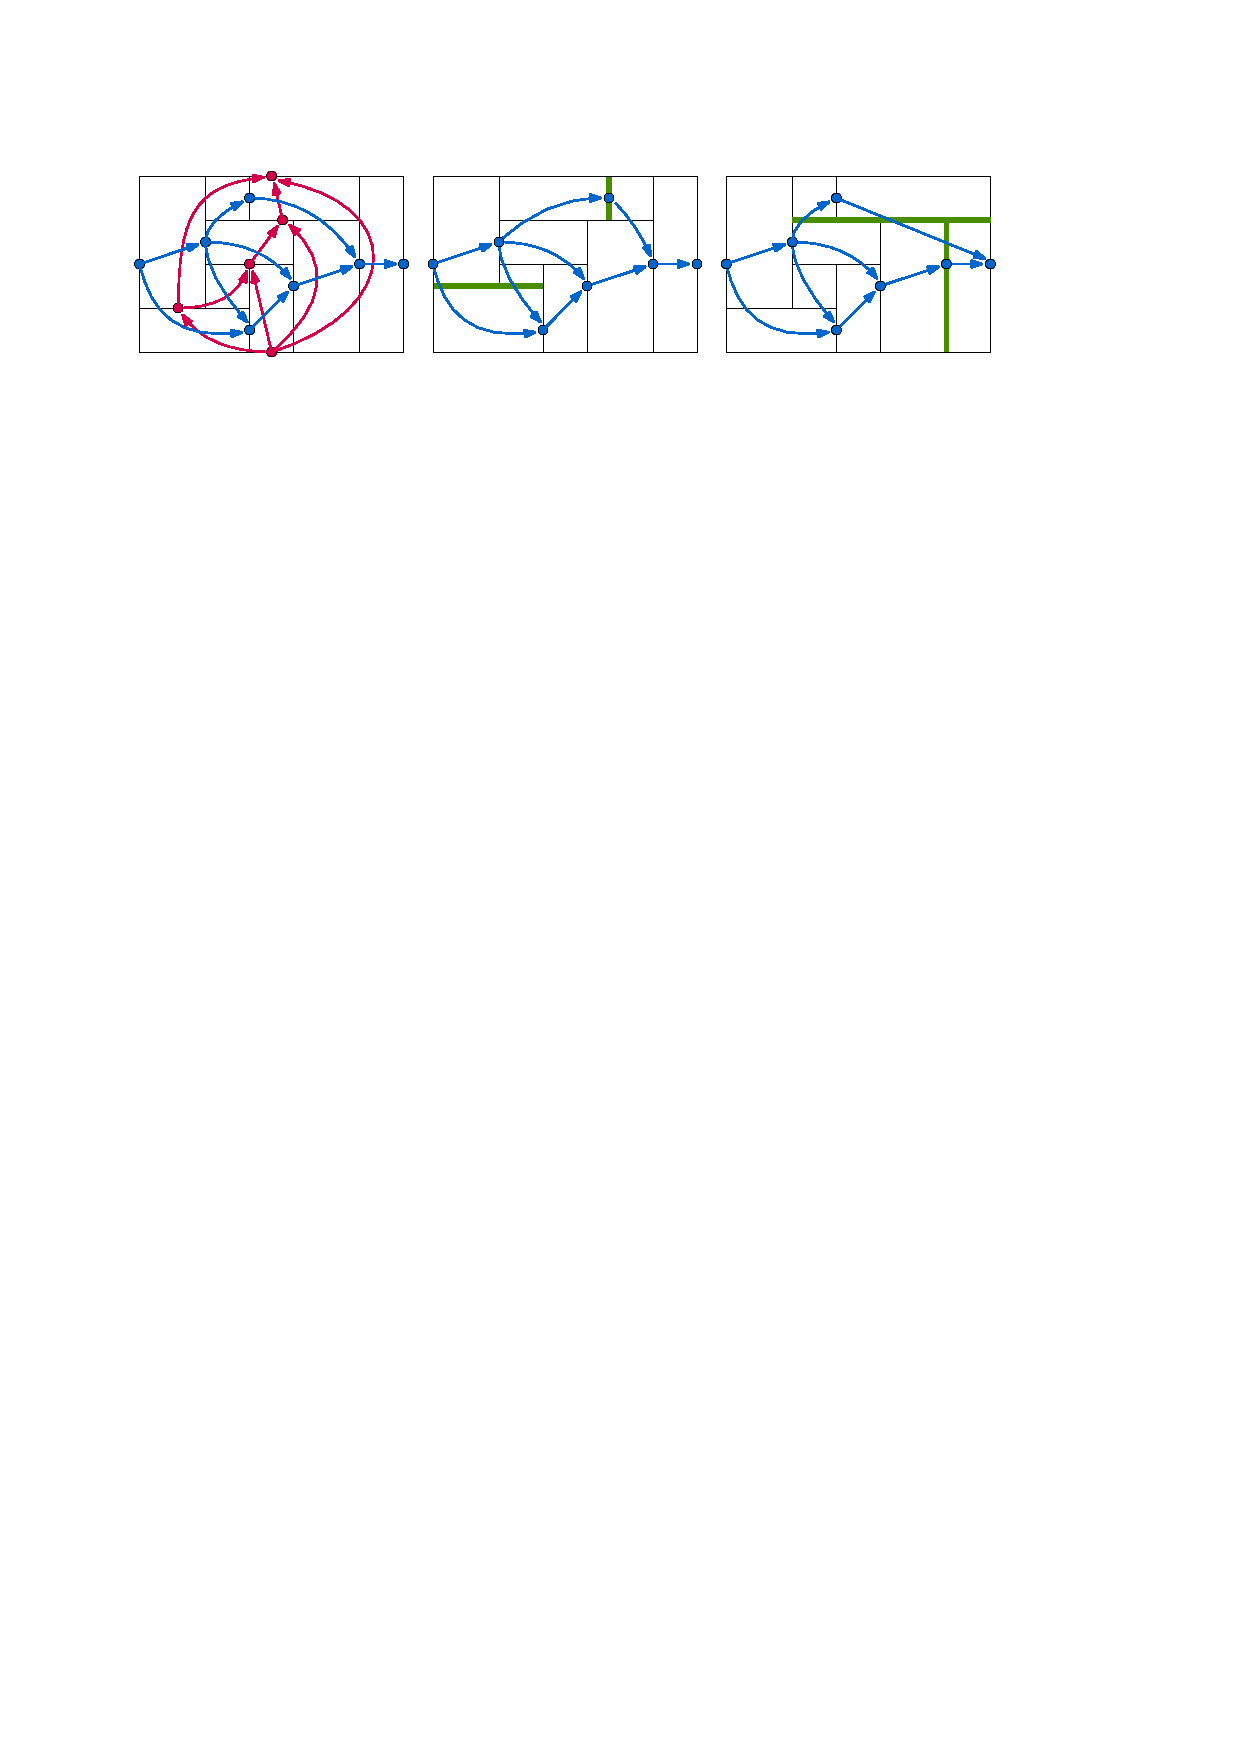
\includegraphics[width=\textwidth]{figures/treemap-evaluation/order-equivalent}
    \caption{Left: Partial orders of the maximal segments. Middle: a layout order-equivalent to the left figure, changed maximal segments highlighted in green. Right: a layout not order equivalent to the other two figures. Red/blue arrows: relations between maximal segments.}
     \label{fig:partialOrder}
\end{figure*}

\mypar{Data change}
%
The stability metrics discussed above do not take data change into account. If data changes by a large amount, then the layouts should be allowed to change significantly without considering this to be instability. To add data change to a stability metric, one can consider the difference or ratio between the layout change and the data change~\citep{vernier18software,vernier18git}.
However, there are two problems: (1) we need a way to measure data change, and (2) the metric spaces for data and layouts need to be comparable. For example, data change can be measured in terms of changes of rectangle \emph{areas} (since these correspond to the data). However, layout changes such as the corner-travel distance measure \emph{lengths}, not areas. Areas and lengths are not directly comparable, and thus their ratios or differences may not be meaningful. 
Although such metrics could be made comparable by suitable normalization, such adaptations are necessarily metric-specific and ultimately result in numbers whose meaning is not clear.% and do not provide a generic solution.

\mypar{Baseline treemap} We overcome the above issues with a new method that captures data change \emph{in the layout space}. For this, we define a \emph{baseline} treemap $T^*$ with respect to $T$ and $T'$. The layout of $T^*$ (that is, the combinatorial structure of the rectangular subdivision which constitutes $T^*$) is based on the layout of $T$. However, the areas of the rectangles in $T^*$ are the areas $\{a'_1, \ldots, a'_n\}$ of $T'$. The idea is that $T^*$ aims to minimize the layout distance to $T$ among all treemaps with the areas of $T'$. Put differently: $T^*$ approximates the minimum amount of change that any time-dependent treemap must incur when moving from $T$ and its associated area values $\{a_i\}$ to the next treemap $T'$ and its area values $\{a'_i\}$. As a result, $d(T, T^*)$ is a good metric for data change in the layout space.

We construct $T^*$ for each tested algorithm and each time step using a hill-climbing algorithm, which was proven to converge in~\cite{eppstein2009area}. For a rectangular layout (treemap) $T$, a \emph{maximal segment} is a maximal contiguous horizontal or vertical line segment contained in the union of the borders of all rectangles in $T$ (for example, the green segments in Figure~\ref{fig:partialOrder}). Put simply, a horizontal maximal segment (which is not part of the input rectangle $R$) always has endpoints on the interior of two vertical segments and vice versa. For two horizontal maximal segments $s_1$ and $s_2$, we say that $s_1 < s_2$ if there is a rectangle in $T$ whose bottom side coincides with $s_1$ and whose top side coincides with $s_2$. This defines a partial order on horizontal maximal segments. We define a partial order on vertical maximal segments analogously (Figure~\ref{fig:partialOrder}). We say that $T$ is \emph{order-equivalent} to $T^*$ if the corresponding partial orders on maximal segments are isomorphic. For every possible set of areas, there exists an order-equivalent treemap to $T$ that correctly represents those areas~\cite{eppstein2009area}. In particular, we can initially define $T^*$ as the treemap order-equivalent to $T$ (computed with any of the tested algorithms) with the areas $\{a'_1, \ldots, a'_n\}$ of $T'$.

If rectangles are inserted or deleted, the baseline treemap cannot be order-equivalent to $T$, so we handle insertions and deletions separately. Dealing with deletions is easy: we simply let the areas go to zero. For insertions, we must be more careful. Indeed, while we consider only rectangles present in both $T$ and $T'$ when measuring stability ($R_i$ and $R_i'$ in Equation~\ref{eqn:delta_ct}), inserted rectangles can strongly impact the positions of rectangles in $T^*$. We observe that the baseline treemap does not need to be a proper treemap: it only needs to capture how much rectangles must minimally move to update to the new data. To minimize the movement of the rectangles due to insertions (and hence be as stable as possible), we distribute the cumulative area of the inserted rectangles over the ``walls'' (borders) of treemap $T$ as evenly as possible. To do so, we replace every maximal segment $e$ in $T$ by a rectangle, and assign each such rectangle a portion of the inserted area corresponding to the length of $e$ (Figure~\ref{fig:baseline}). Hence all walls become equally thick and the original rectangles of $T$ need to move as little as possible to yield $T^*$.

The baseline treemap $T^*$ as proposed here is not a perfect baseline, as it does not always minimize the movement of every rectangle. However, the layout change between $T$ and $T^*$ is still a very good estimate for the minimum necessary layout change between $T$ and $T'$, and thus a good measure for data change (see Figure~\ref{fig:CTDvsBase}: nearly all points lie on or below the diagonal). 
% Also, note that $T^*$ is not an actual treemap that represents the input data. Instead, $T^*$ it is an artificially created treemap (thus, the name `baseline'), which has many additional (gray) rectangles that represent the data change between time steps.

%
\begin{figure}[ht]
\centering
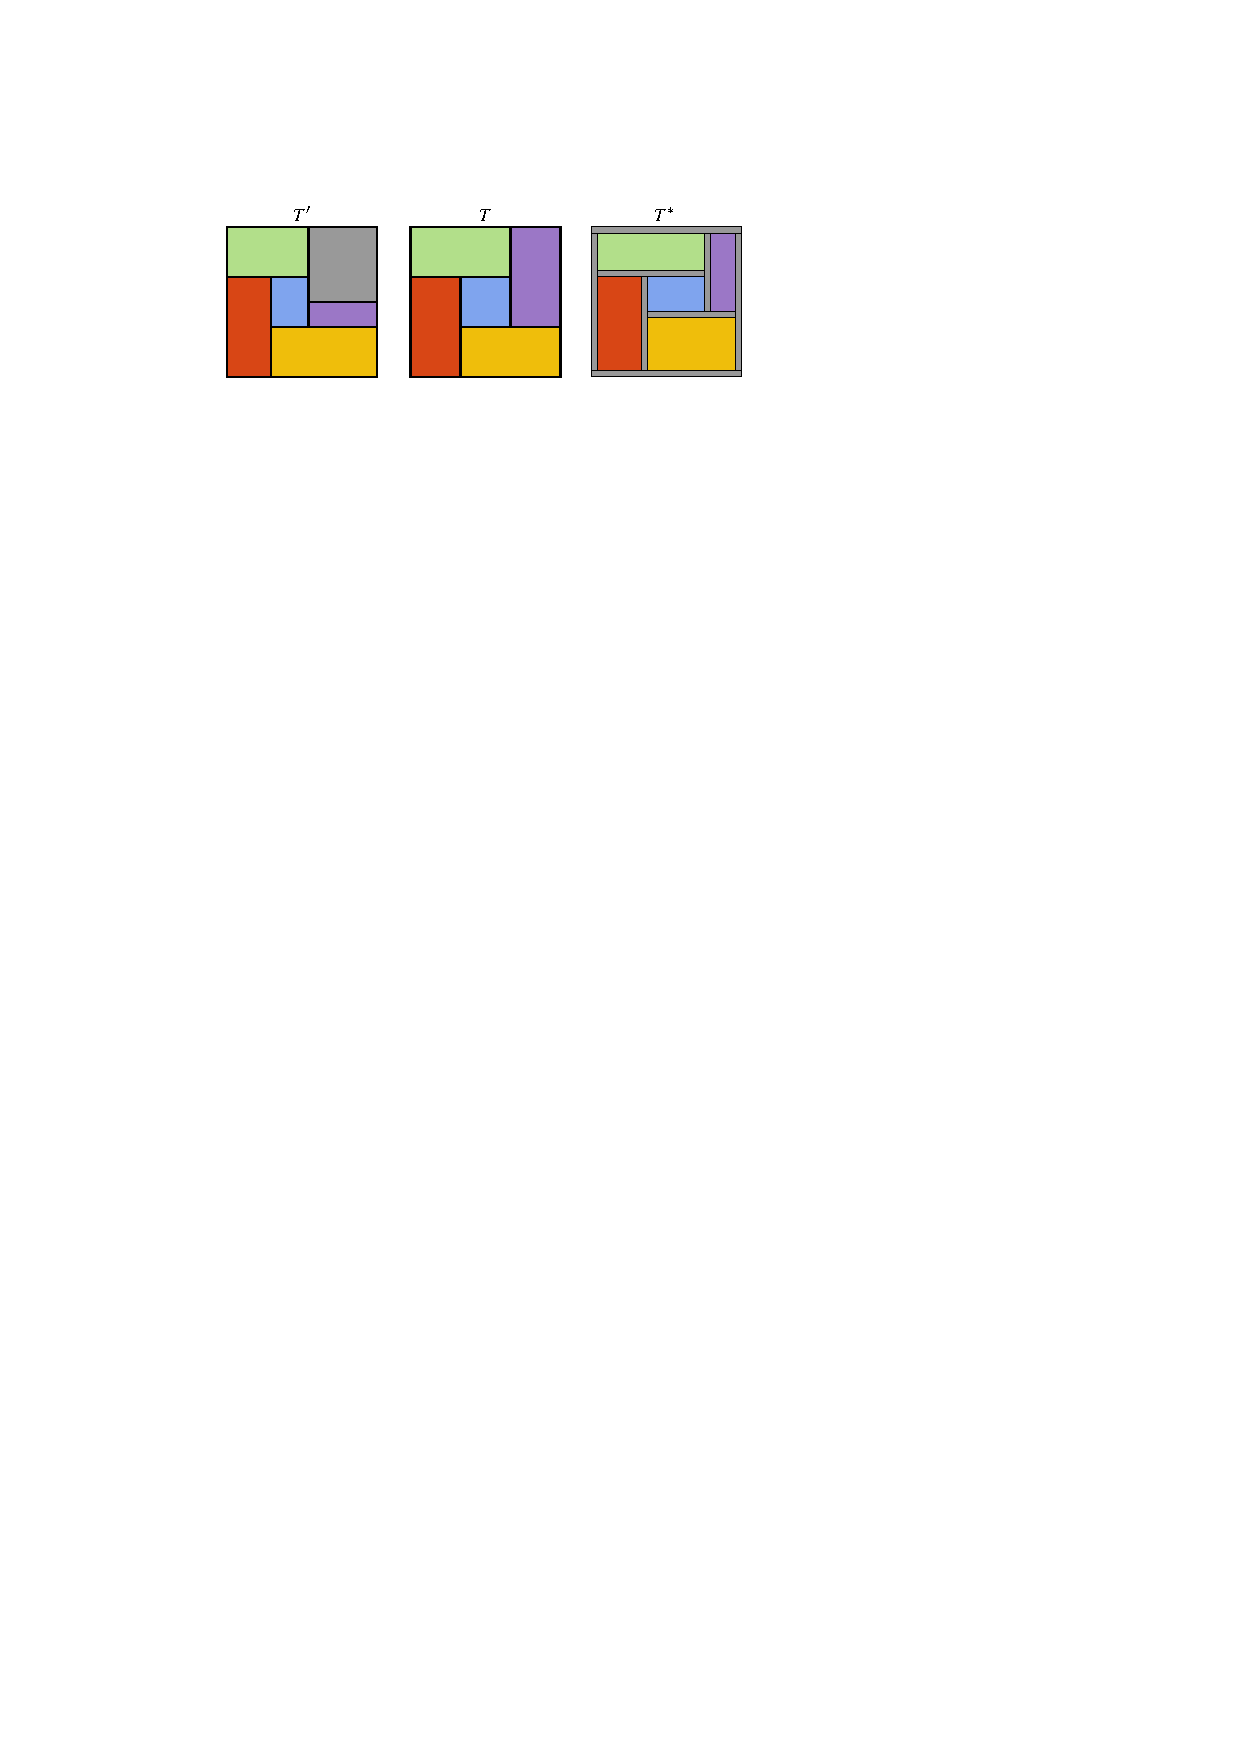
\includegraphics[width=.8\textwidth]{figures/treemap-evaluation/baselineRow}
    \caption{Treemaps $T'$ (with gray rectangle inserted), $T$, and $T^*$ (with gray area spread over maximal segments).}
     \label{fig:baseline}
\end{figure}
%

\begin{figure}[ht]
    \centering
    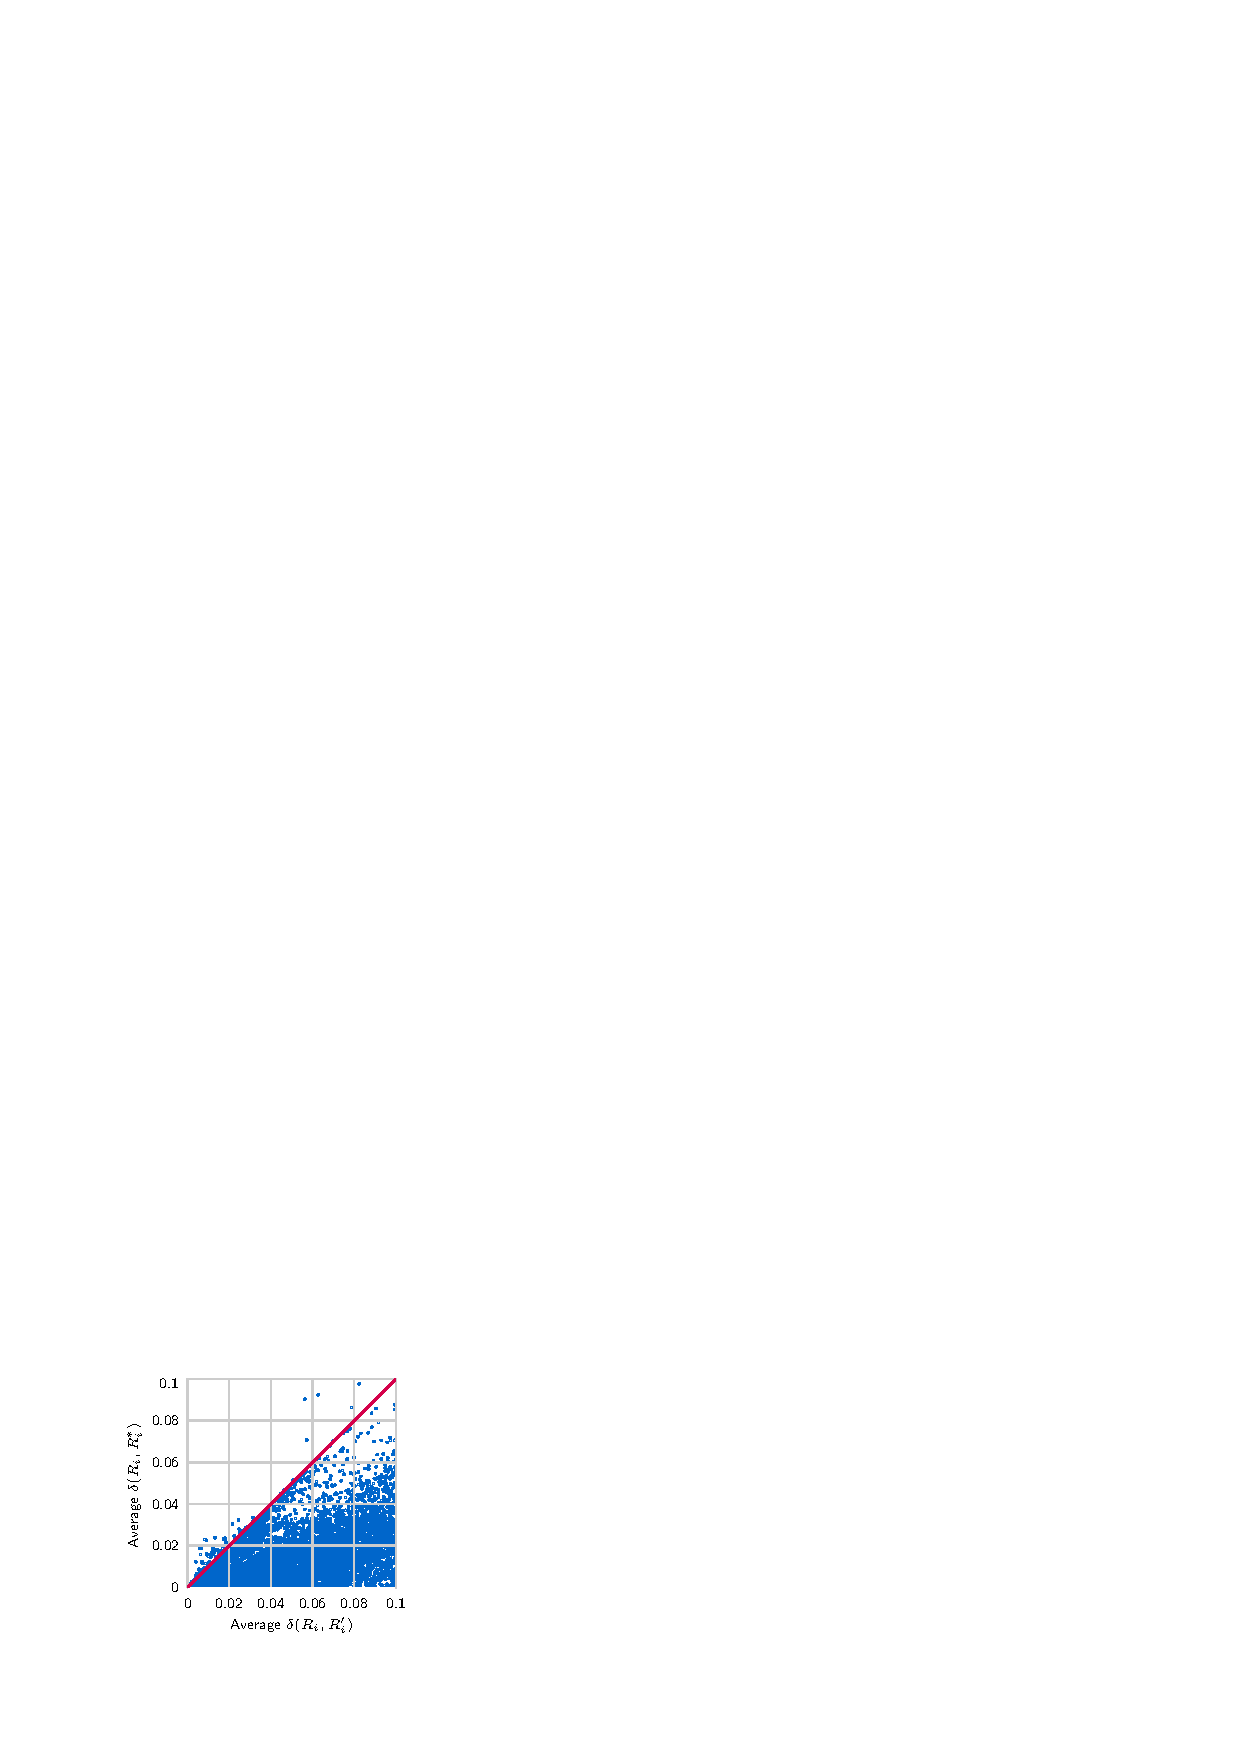
\includegraphics[width=.5\textwidth]{figures/treemap-evaluation/BaselineVerificationv5}
    \caption{Scatter plot of the average layout change between $T$ and $T'$ or $T^*$ for a random 25\% sample of all algorithms and datasets.}
    \label{fig:CTDvsBase}
\end{figure}

\mypar{Stability metric}
We can now define a stability metric that takes data change into account. Consider a rectangle $R_i$ and the corresponding rectangles $R'_i$ and $R^*_i$ in $T'$ and $T^*$, respectively, and let $\delta$ be the layout change function for single rectangles. Two natural choices for spatial stability are the difference or ratio between $\delta(R_i, R'_i)$ and $\delta(R_i, R^*_i)$. Our experiments showed that the difference is typically more informative, that is, it exhibits clearer, more pronounced patterns, than the ratio. Hence, we define the stability of a single rectangle 
% the corner-travel distance 
as
%
\begin{align}
\sigma(R_i) &= \max(0, \delta(R_i, R'_i) - \delta(R_i, R^*_i)) \label{eqn:sigma_ct}
\end{align}
%
Note that $\sigma(R_i) = 0$ if $\delta(R_i, R'_i) \leq \delta(R_i, R_i^*)$, which is possible. Indeed, a value of $0$ for $\sigma(R_i)$ represents ``very stable'', and $R_i^*$ is considered to be (roughly) as stable as possible.

\mypar{Limitations} The stability metrics we use focus only on consecutive time steps. The stability of time-varying treemaps could conceivably be influenced by effects that span multiple time steps, which our metrics do not capture directly. However, we believe that the most salient events influencing stability occur between consecutive time steps and hence we focus on this scenario.


\section{Data}
\label{sec:data}
%
The visual quality and/or stability of treemaps clearly depends on the datasets used. Simply measuring the average performance over a (large) collection of datasets does not reveal such information. We aim to provide sufficient insight so that both practitioners and researchers can make informed choices about which algorithm to use for their data. For this, we study the performance of treemaps as a function of the characteristics of the input data. We classify the datasets into data classes along with explicit features and evaluate the metrics of different treemapping algorithms for each class. 

\subsection{Data features}
\label{sec:dataspace}
%
Our methodology is inspired by the framework proposed by \cite{smith2014towards} to objectively measure the performance of algorithms across datasets. For each dataset, we compute a number of features that (hopefully) capture the characteristics influencing the relative performance of treemapping algorithms. As a result, every dataset is represented by a point in a low-dimensional \emph{feature space} $\mathcal{F}$. Similar feature-based approaches are also used to measure the relative performance of dimensionality-reduction methods~\citep{Espadoto19} or in machine learning~\citep{bishop06}. Based on the discussion of treemapping algorithms in Section~\ref{sec:algorithms-2}, we identify the following four features: \textbf{1.} Levels of hierarchy, \textbf{2.} Variance of node weights, \textbf{3.} Weight change, and \textbf{4.} insertions and deletions.


Obviously, other features could be used to characterize (time-dependent) trees, such as the minimum, maximum, and average node degrees, the (im)balance of the tree structure~\citep{boorman73,kuhner14}, and the number of nodes. Two seemingly obvious candidates for features that we do not currently consider are the \emph{number of nodes} and the \emph{branching factor} (i.e., the average internal node degree). Arguably the number of levels in the hierarchy, the branching factor, and the number of nodes correlate to some degree. For example, if the hierarchy has only one level, then the branching factor and the number of leaves are the same. Hence, we should include at most two of these features in our analysis. Among these three features, the number of levels is with certainty a discriminating factor between algorithms, see our discussion in Section~\ref{sec:algorithms-2}. Furthermore, all algorithms we consider, with the exception of SND, are recursive and treat each level independent from the preceding ones. Hence one can argue that the branching factor, which determines the number of nodes that have to be handled during a single step of this recursion, is a more relevant data feature than the total number of nodes. Nevertheless, we decided not to include the branching factor in our experiments, for the following two reasons. First of all, from the description of the algorithms, it seems that the branching factor is likely less relevant for their \emph{relative} performance than the other four chosen features. That is, the descriptions of the algorithms do no give an indication that the branching factor is able to predict if an algorithm $A$ will perform better than an algorithms $B$ on a given dataset. Second, it is very difficult to define  meaningful value-ranges for the branching factor and then to find datasets that cover these ranges in combination with all other data features. Given that the number of data classes and, correspondingly, the number of datasets needed for a meaningful evaluation, grows exponentially with the number of features chosen (see Section~\ref{sec:datasampling}), we decided to restrict ourselves to four features. While we cannot exclude that the branching factor may influence relative performance, we do believe that the four features chosen have higher predictive value.

%While such features will influence performance aspects of treemaps such as running time, we believe they are less discriminative for treemaps. Separately, we must limit the number of features used to describe $\mathcal{F}$ to make analysis of feature type the sampling thereof practical in terms of the number of resulting datasets, and further quality computations done on these, as outlined next.

\subsection{Data classes}
\label{sec:datasampling}
%
Using the feature space $\mathcal{F}$, we partition all datasets into classes. For each feature we define a small number of subclasses based on only that feature. The data class of a dataset is then defined as the combination of the subclasses for each feature. We determined the value-ranges defining the subclasses by analyzing the distribution of feature values over our 2405 real-world tree datasets.  

%\todo{Add a bit more to this, couple to the algorithms directly.}

\mypar{Levels of hierarchy (3 subclasses)} We use three ranges for classification: 1 level (1L), 2 or 3 levels (2/3L), and more than 3 levels (4+L). Most hierarchical datasets we have analyzed have 2 or 3 levels. This number of levels is quite common for datasets that are visualized via treemaps, since they frequently concern geo-spatial subdivisions such as countries, continents, and their subregions, grouped by a classification scheme, such as the World Bank regional classification. Furthermore, visually understanding the node nesting in deeper treemaps becomes difficult~\citep{vliegen,sqr}.
% or the United Nations geoscheme. 
% mainly because visually understanding the node nesting in deeper treemaps becomes difficult~\citep{vliegen,sqr}. This is also recognized by Tableau\footnote{Tableau visualization software. \url{www.tableau.com}} where treemaps having more than a few levels are not explicitly supported by visual cues. 
A special case are datasets with only 1 level, that is, sets of weight values. Such datasets are also often visualized by treemaps, as these are more space-filling than alternatives such as bar charts~\citep{vliegen}. These datasets are challenging for treemaps that implicitly use the depth of the hierarchy. Finally, we consider datasets with more than 3 levels, which correspond to deep hierarchies such as, for example, file systems or software architectures~\citep{hahn10,Hahn2017,vernier18software}.

\mypar{Variance of node weights (2 subclasses)} We distinguish between low variance (LWV) and high variance (HWV). To ensure that the total number of tree nodes does not strongly influence our classification, we use the coefficient of variation $\sigma/\mu$ to determine the subclass. The standard deviation $\sigma$ and the mean $\mu$ are computed over all leaf weights over all time steps. We say that there is low variance if $\sigma/\mu \leq 1$ and high variance if $\sigma/\mu > 1$, respectively.

\mypar{Weight change (3 subclasses)} We distinguish between low weight change (LWC), regular weight change (RWC), and spiky weight change (SWC). The weight change of a single rectangle is measured by the absolute difference in the relative area (with respect to the input rectangle R) between time steps. The weight change of a treemap between two time steps is defined as the sum of weight changes of all rectangles. To determine the subclass of a dataset, we use the distribution of weight changes between time steps over all time steps in the dataset, specifically the mean $\mu$ and the standard deviation $\sigma$. Datasets with low weight change have $\mu < 5\%$ and $\sigma < 5\%$. Datasets with a larger mean ($5\% \leq \mu < 20\%$) and a relatively small coefficient of variation ($\sigma/\mu \leq 1$) are classified as having regular weight change. The weights of these datasets steadily change over time, without any extreme changes. Remaining datasets are classified as having spiky weight change. In those datasets weights change drastically ($\mu > 20\%$), or there is large variation ($\sigma/\mu > 1$) along with substantial changes ($\mu > 5\%$ or $\sigma > 5\%$). 

%Let $\mathcal{A}^+$ denote the set of nonzero weights at two consecutive time steps $t$ and $t+1$, and let $A^+(t)=\sum_{\mathcal{A}^+} a_i(t)$ and $A^+(t+1) = \sum_{\mathcal{A}^+} a_i(t+1)$ be the sum over all $a_i(t)$ and $a_i(t+1)$, respectively, for those $a_i$ that are in $\mathcal{A}^+$. We measure the weight change between $t$ and $t+1$ as $WC(t) = \sum_{\mathcal{A}^+} |a_i(t)/A^+(t) - a_i(t+1)/A^+(t+1)|$. We define the weight change as small if both the mean and standard deviation of $WC(t)$ over all time steps $t$ are less than $5\%$. In this case, the dataset's weight changes are small with few outliers present. We define the weight change as regular if the coefficient of variation $\sigma/\mu$ of $WC(t)$ is at most 1, the mean is less than $20\%$, and the weight change is not small. In this case, significant changes happen but the number of outliers is small. Finally, we define the weight change as spiky if it is not small nor regular. In this case, either very large changes ($\mu > 20\%$) continuously occur, or the coefficient of variation is large ($\sigma/\mu > 1$) and changes are somewhat substantial ($\mu > 5\%$ or $\sigma > 5\%$).

\mypar{Insertions and deletions (3 subclasses)} We distinguish between low insertions and deletions (LID), regular insertions and deletions (RID), and spiky insertions and deletions (SID). We measure the impact of insertions and deletions between two time steps $t$ and $t+1$ as the cardinality of the symmetric difference between the two sets of rectangles with non-zero weights at $t$ and $t+1$, divided by the number of rectangles with non-zero weights at $t$. We again classify the datasets based on the distribution ($\mu$ and $\sigma$) of impact values over all time steps. Same as for the weight change, LID is defined by $\mu < 5\%$ and $\sigma < 5\%$, RID is defined by $\mu < 20\%$ and $\sigma/\mu \leq 1$, and the remaining datasets are in SID. 


%For two consecutive time steps $t$ and $t+1$, let $\mathcal{A}^+(t)$ and $\mathcal{A}^+(t+1)$ denote the set of non-zero weights at $t$ and $t+1$, respectively. We measure the impact of insertions and deletions $ID(t)$ as the cardinality of the symmetric difference between $\mathcal{A}^+(t)$ and $\mathcal{A}^+(t+1)$, relative to the cardinality of $\mathcal{A}^+(t)$, that is, $ID(t) = \lvert\mathcal{A}^+(t) \oplus \mathcal{A}^+(t+1)\rvert / \lvert\mathcal{A}^+(t)\rvert$. As above and with the same reasoning, we denote the impact of insertions and deletions as small if both the mean and standard deviation of $ID(t)$ over all time steps $t$ is less than $5\%$; we denote it as regular if the coefficient of variation $\sigma/\mu$ of $ID(t)$ is at most 1, its mean is less than $20\%$, and the data is not classified as small; and we denote the impact as spiky if it is not classified as small nor as regular.



\medskip
\noindent
The full classification results in $3 \times 2 \times 3 \times 3 = 54$ data classes. In Section~\ref{sec:exploration}, we evaluate how the performance of treemapping algorithms depends on the classes, that is, if the classification is sensible. 

%This sampling of $\mathcal{F}$ yields $3 \times 2 \times 3 \times 3 = 54$ dataset categories. We next describe how we practically executed a sampling of $\mathcal{F}$ along this grid to evaluate treemap performance.


\subsection{Datasets}
\label{sec:datasets-2}
%
We collected a total of 2405 time-dependent hierarchical datasets from a variety of sources, detailed below. We found at least one dataset for 46 (out of 54) instances of our proposed data classes. See Figure~\ref{fig:datasets_summary} for the distribution of datasets over classes: clearly not all classes arise with equal frequency in our data sources.

\begin{figure}[t]
    \centering
    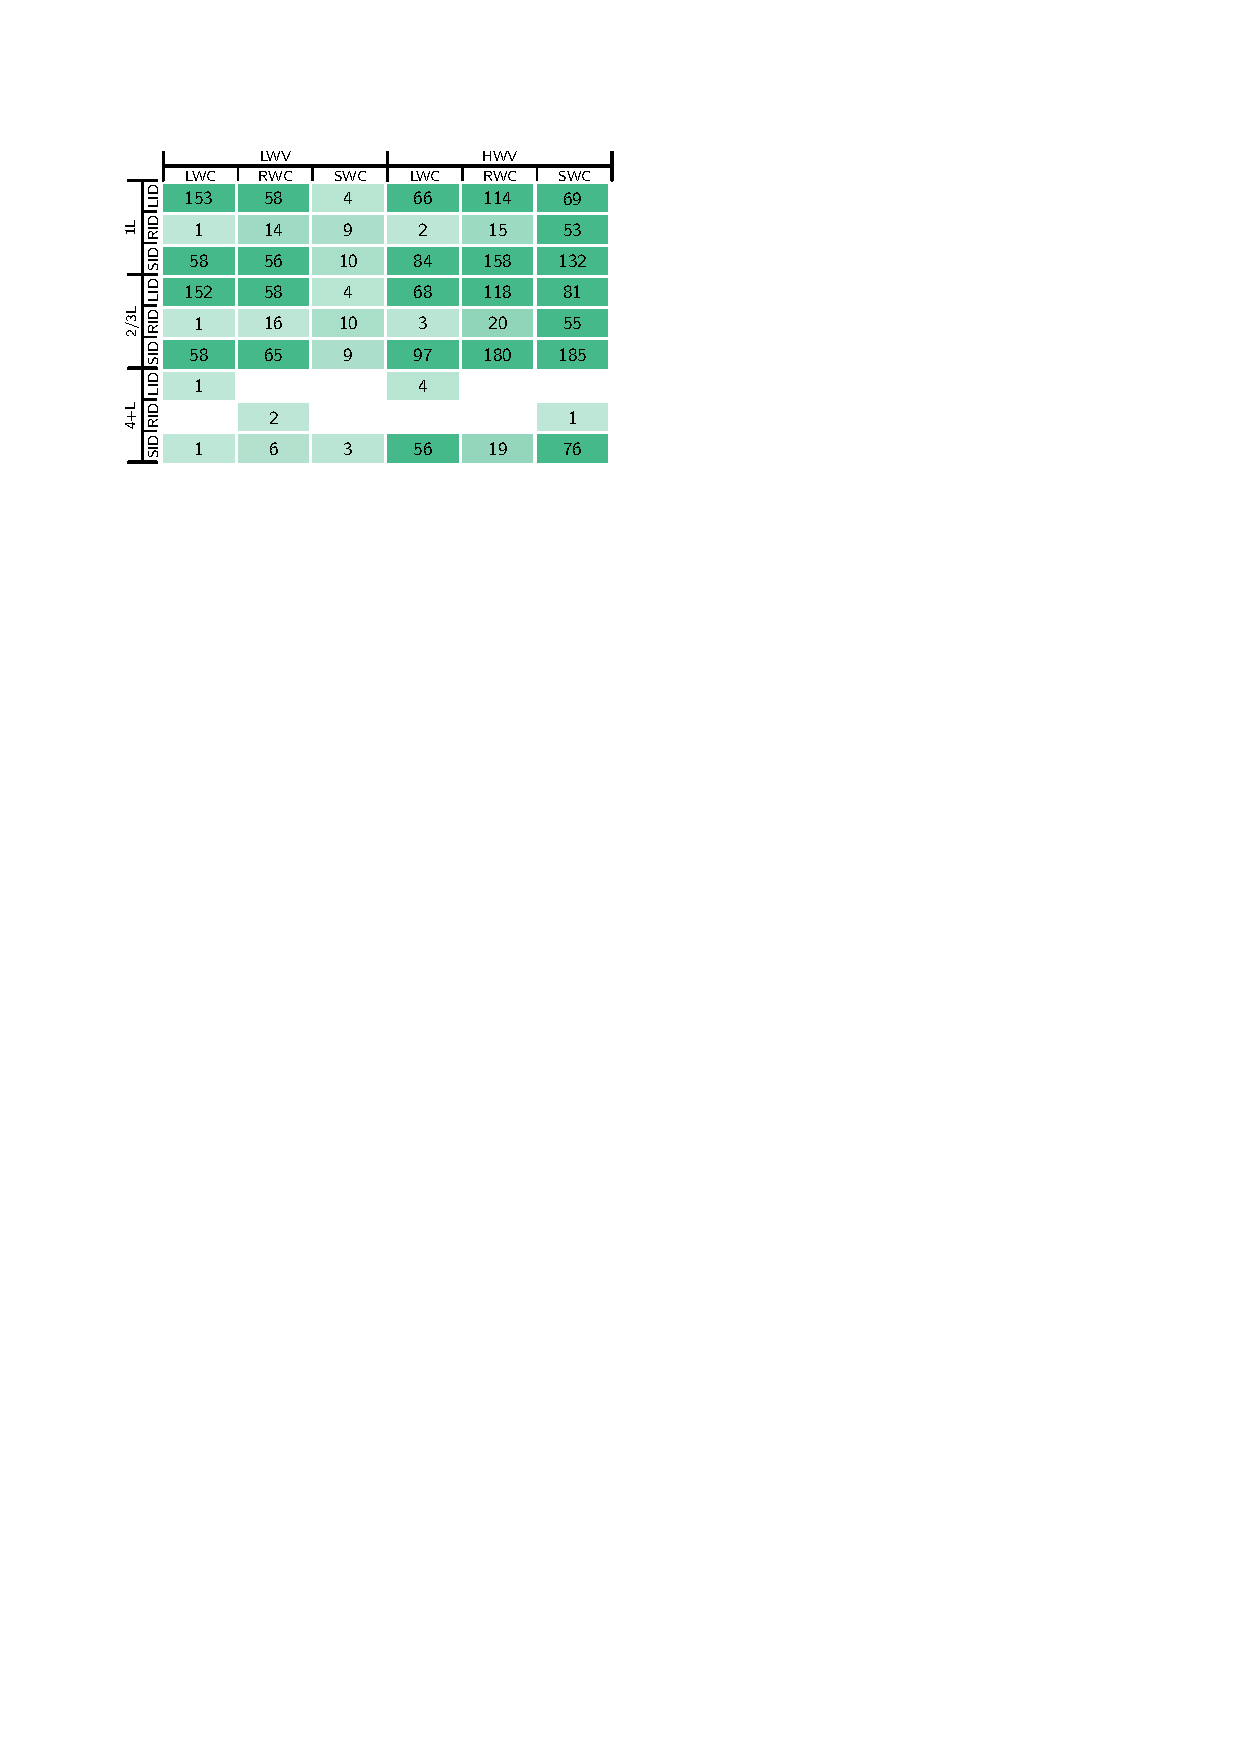
\includegraphics[width=.7\textwidth]{figures/treemap-evaluation/count}
    \caption{Distribution of datasets over classes.}
    \label{fig:datasets_summary}
\end{figure}

\begin{description}
\item[World Bank \citep{URLWorldbank}:] (2142 datasets) World development indicators such as agriculture, rural and urban development, education, trade and health. Hierarchy either according to the World Bank regional classification, grouping countries into subregions and continents, or no hierarchy present.
\item[GitHub \citep{URLGit}:] (150 datasets) Hierarchies of folders, files, and classes, weighted by the number of code lines, extracted from all revisions of several GitHub repositories using Scitools~\citep{URLscitools}.
\item[Movies:] (107 datasets) Movies from MovieLens \citep{harper2016movielens} and \emph{TMDB}~\citep{URLmdb}. We constructed a time-dependent hierarchy using the group-rows-by-attribute-value partitioning method~\citep{tablelens,vliegen}. The hierarchy groups movies based on their genres, actors, release date, and keywords. Each leaf is a movie, whose weight corresponds to its rating over a given period of time.
%stores a statistical measure (sum, mean, standard deviation, or count) of that movie's ratings over a given period of time.
\item[Custom:] (6 datasets) Several individual datasets were added: %to widen the provenance areas of our data.
%We added several hand-picked datasets to cover classes that did not appear in the automatically mined datasets:
\emph{Dutch Names}~\citep{urlmeertens} contains the frequency of popular baby names in the Netherlands per year; \emph{UN Comtrade Coffee}~\citep{URLComtrade} contains the amount of coffee each country imported per year; \emph{ATP} contains personal information, historical rankings, and match results from 1968 to 2018 for ATP tennis players~\citep{URLatp}; and \emph{Earthquakes} contains the time, location, depth and intensity of seismic phenomena provided by the USGS Earthquake Hazards Program~\citep{URLearth}.
%, and also to widen the provenance areas of our data.
\end{description}
%
Importantly, note that the above selection of dataset sources is \emph{orthogonal} to the description of the feature space $\mathcal{F}$. The former covers the \emph{origin} of data (which may cover application-specific aspects not captured by our feature space); the latter covers application-independent data aspects as captured by the data classes of $\mathcal{F}$. The distributions of data classes covered by our different data sources can be found in the supplementary material. The large and varied collection of World Bank datasets is able to cover all data classes with at most 3 levels of hierarchy (to which it is inherently limited). The GitHub and Movies datasets further cover a number of data classes with 4+ levels of hierarchy. 

% To collect data from World bank, GitHub, MovieLens, and TMDB, we wrote several automation scripts to download the raw data, filter it to eliminate unusable (corrupted) datasets, create the hierarchies by grouping and binning data entries as needed, and finally compute the data features (Sec.~\ref{sec:data}).


\section{Experimental Results}
\label{sec:exploration}

We ran all 14 algorithms on all time steps of all 2405 datasets, generated the baselines for all these instances (Section~\ref{sec:metrics-2}), and recorded all layouts, that is, the positions of all rectangles $R_i(t)$ at all time steps $t$. Per dataset we aggregate our results for all metrics and algorithms by first by taking the mean over all rectangles in a single time step, and then by taking the mean again over all time steps. This is necessary since the number of rectangles may differ per time step. 

%This data (about 100GB) serves as the basis for our analysis, further described in this section.

% \todo{Mean/median and aspect ratio is too long. Should be compressed.}

% Due to the large amount of data, we need to aggregate our metrics to be able to analyse our results. As both the visual quality and stability metrics are defined on a  rectangle level, we aggregate them in the same way.
% We first take the mean over all rectangles in a single timestep. This gives us a score that is independent of the amount of nodes. We then take the mean over all timesteps, which gives a score independent of the amount of timesteps. We use this score as our basis for comparison. Thus we have a single score for every algorithm run on each dataset. 

% Alternatively, instead of the mean we could have used the median to aggregate the metrics. The main advantages of using the median is that it is more robust against outliers, which would allow us to use the non-inverted aspect ratio, which is easier to parse but prone to outliers. When doing this we however lose too much resolution in the data for meaningful comparison. Often, especially for stability, a large amount of rectangles have very low scores, but a long tail is present in the distribution which should not be simply ignored.

We focus on two specific questions: We first explore the \emph{validity} of our data classification (Section~\ref{sec:validity}) and then we study the \emph{performance} of all algorithms with respect to visual quality and stability across varying data features (Section~\ref{sec:acrossfeatures}).
In the supplementary material we additionally compare the performance of all algorithms on each data \emph{class} separately. We believe that the resulting visual summary will help researchers and practitioners choose a suitable treemapping algorithm for their data.

\begin{figure}[ht]
    \centering
    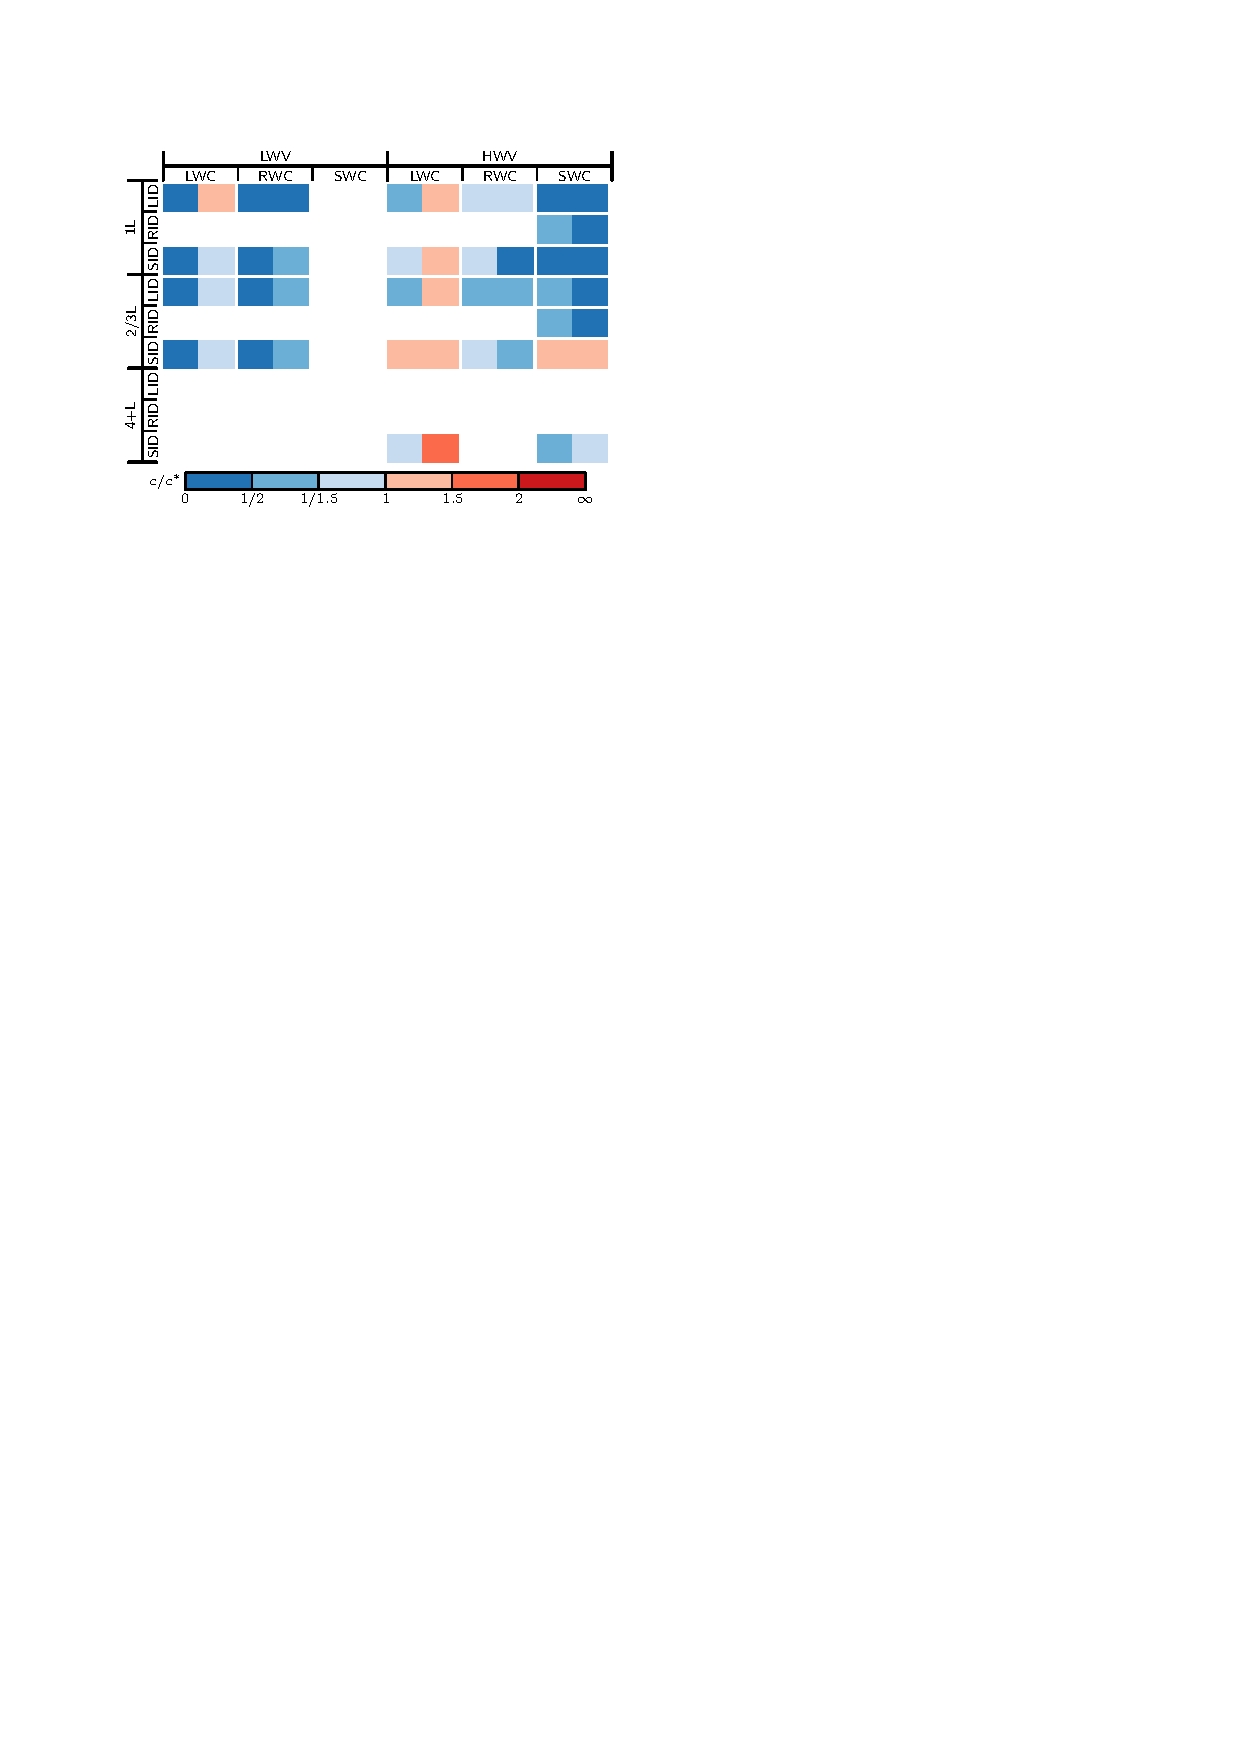
\includegraphics[width=.7\textwidth]{figures/treemap-evaluation/VarianceTable}
    \caption{For each data class with at least 50 datasets, the ratio of the consistency score (visual quality on the left, stability on the right) between the data class and the baseline. }
    \label{fig:variancetable}
\end{figure}

\begin{sidewaysfigure}
% \begin{figure*}[]
    \centering
    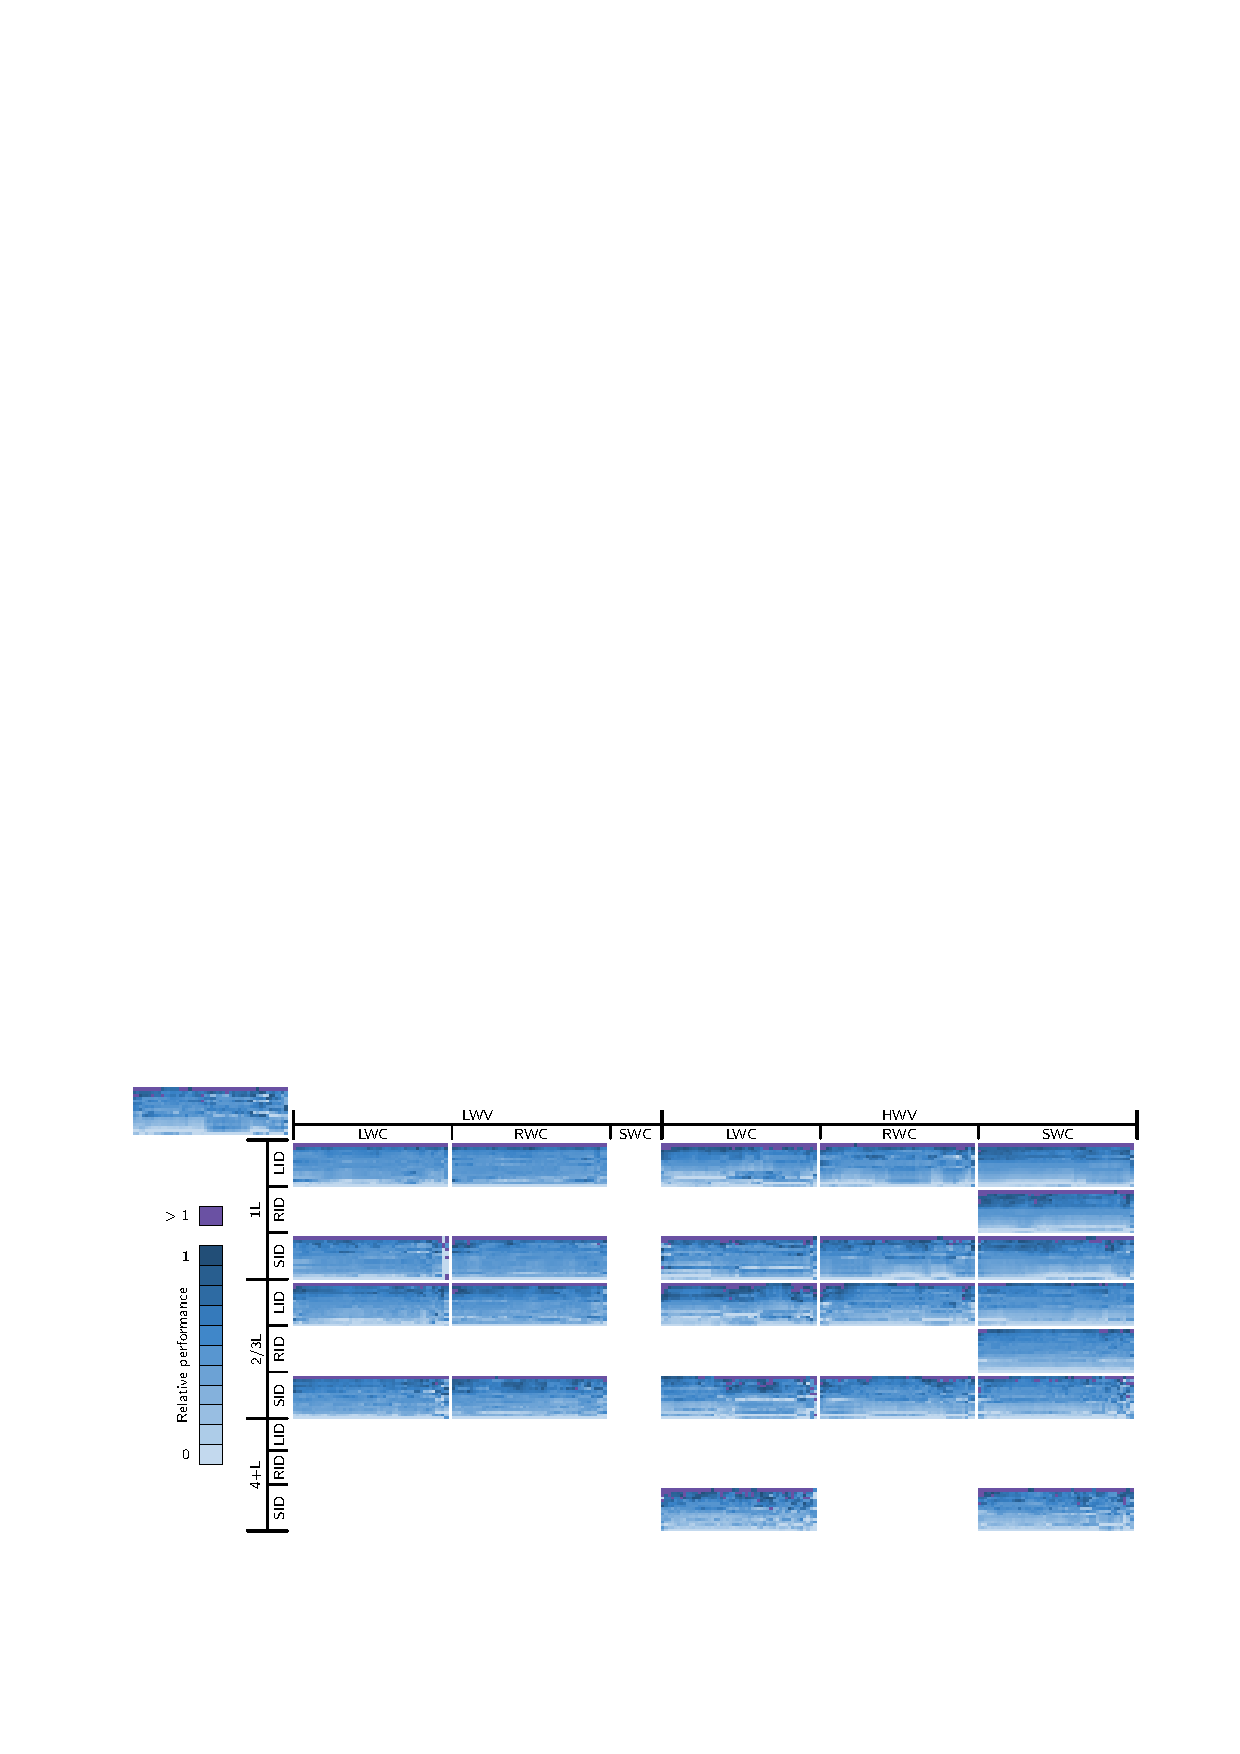
\includegraphics{figures/treemap-evaluation/MeanArRug}
    \caption{Visual quality: matrix plots for each data class with at least 50 datasets plus baseline (left top). In each matrix plot, rows correspond to algorithms, columns to datasets. The lighter the color, the better the relative performance, capped at 1 (purple).}
    \label{fig:meanrug}
% \end{figure*}
\end{sidewaysfigure}


\begin{sidewaysfigure}
% \begin{figure*}[]
    \centering
    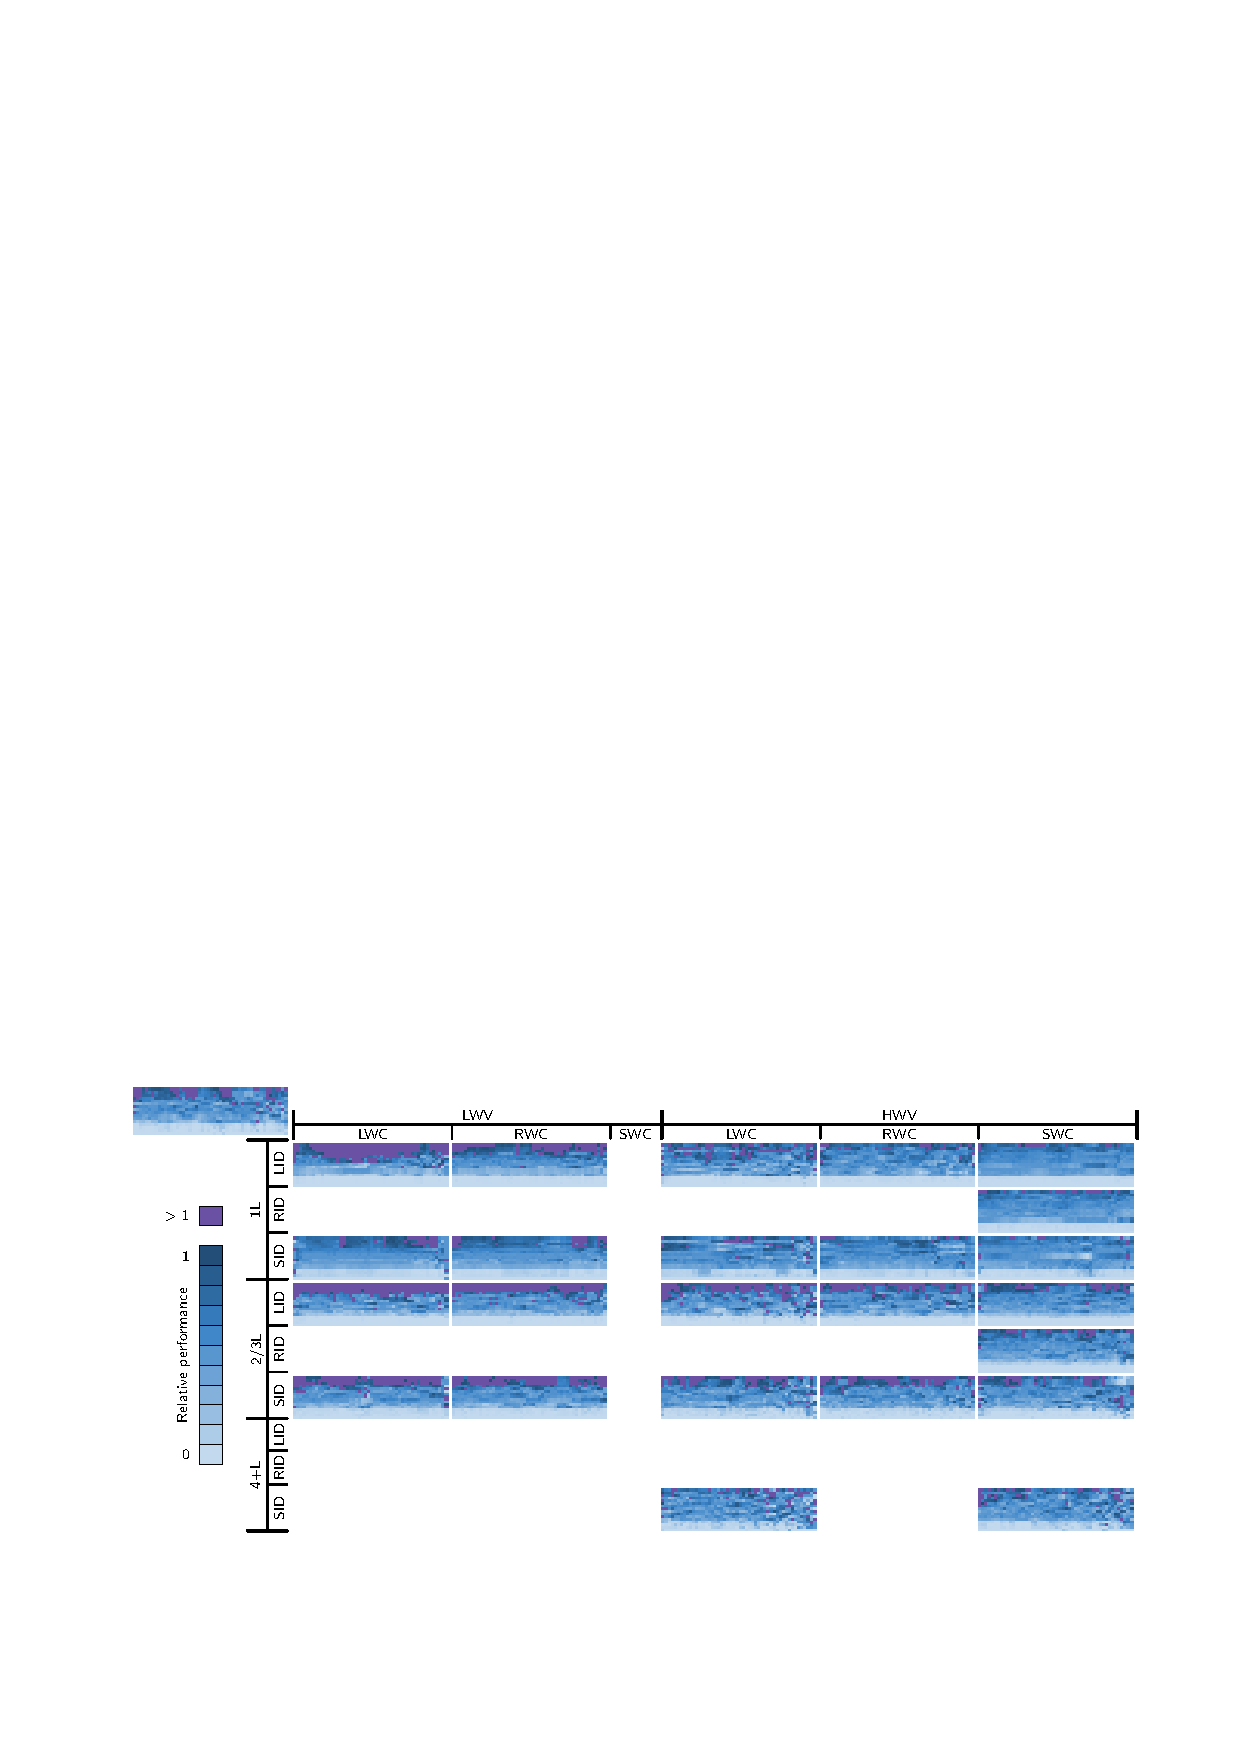
\includegraphics{figures/treemap-evaluation/baseCTDRug}
    \caption{Stability: matrix plots each data class with at least 50 datasets plus baseline (left top). In each matrix plot, rows correspond to algorithms, columns to datasets. 
    The lighter the color, the better the relative performance, capped at 1 (purple).}
    \label{fig:ctdrug}
% \end{figure*}
\end{sidewaysfigure}


\subsection{Data classification analysis}\label{sec:validity}

We evaluate if the relative performance of treemapping algorithms is more consistent within a data class than for an arbitrary collection of datasets. To perform this analysis we need to establish how we can capture the consistency of relative performance for a collection of datasets, and how we can compare this consistency between multiple collections. 
%
We restrict our analysis to data classes that contain at least 50 datasets, for otherwise the observed consistency is not sufficiently reliable. For each such data class, we randomly sample 50 datasets to use in this analysis. We also randomly sample 50 datasets among all 2405 datasets (all classes) as a baseline for comparison. Note that all collections must have the same number of datasets in the analysis to ensure that the comparisons are fair.

Now consider a single collection of datasets. To measure the consistency of relative performance among different datasets in this collection, we cannot directly use the computed metrics for visual quality and stability, as these values may differ greatly between datasets. Alternatively, we could rank the algorithms per dataset, but then algorithms with very similar performance may imply a greater variance in relative performance than is the case. Instead, we define the \emph{relative performance} (separately for visual quality and stability) per dataset as follows. We compute both the best value (maximum for visual quality, minimum for stability) and the median value over all algorithms over this dataset. The \emph{relative performance score} for each algorithm on this dataset is then computed by linearly interpolating between these two values, where the best algorithm receives score $0$, and the median algorithm receives score $0.5$. The relative performance score is capped at $1$, to avoid outliers. The resulting scores are comparable between different datasets.



We next analyze the consistency of relative performance within collections of datasets in two different ways. First, we use a quantitative approach: for each algorithm we compute the variance of the relative performance scores over all datasets in a collection, and we sum up these variances over all algorithms. This results in a \emph{consistency score} $c$ for a collection of datasets. Figure~\ref{fig:variancetable} displays the consistency scores (for visual quality and stability) of all data classes (with at least 50 datasets) compared to the consistency scores $c^*$ of the baseline collection (created by random sampling). A cell is colored blue (more consistent) if $c$ is smaller than $c^*$; a cell is colored red (less consistent) if $c$ is larger than $c^*$.

Nearly all data classes for visual quality and most data classes for stability are more consistent than the baseline. This indicates that our features are splitting the datasets into valid data classes where the relative performance of an algorithm is easier to predict than in the baseline.
However, the stability column for high weight variance and low weight change is less consistent than the baseline. As discussed in Section~\ref{sec:algorithms-2}, the stability of unordered treemaps becomes worse compared to ordered treemaps when the weight variance is low or the weight change is high, due to reordering of the input weights. As a result, the difference with respect to stability between ordered and unordered treemaps is less pronounced for these data classes; the relative performance is hence influenced more by accidental details of individual datasets and less by structural differences between the algorithms. Additionally there are two data classes where the visual quality is less consistent than the baseline. 
%These two classes both have height weight change, 2/3 levels, and spiky insertions and deletions. 
It is not clear to us at this point what the cause of these inconsistencies is; one possibility are hidden correlations in the data classes.

Second, we use a more qualitative approach to assess the consistency of relative performance. For each data class we create a matrix plot, that shows the relative performance scores of all algorithms for all datasets in the collection (see Figures~\ref{fig:meanrug} and~\ref{fig:ctdrug}). Each column in the matrix plot represents a dataset, and each row represents an algorithm. The color of every ``cell'' in the matrix plot indicates the relative performance score of an algorithm on a dataset, where lighter colors indicate better (lower) relative performance scores. Relative performance scores that were capped at $1$ are indicated with purple. To better enable the visual assessment of consistency among the different datasets in a collection, we order the datasets (columns) so that those with similar scores are next to each other as much as possible. Also, we order the algorithms (rows) so that the algorithms with better average score are lower in the matrix plot. In particular, the order of algorithms in the matrix plots for different data classes can be different. Figure~\ref{fig:meanrug} shows the matrix plots for visual quality, with the corresponding matrix plot for the baseline collection at the left-top. Figure~\ref{fig:ctdrug} shows the matrix plots for stability.

% brightness = 85-relativePerformanceScore*55. (score =1 => outlier)
%HSB color scale

First consider the matrix plot for visual quality (Figure~\ref{fig:meanrug}). For the low weight variance subclass we indeed see that the matrix plots are much smoother than the baseline, which confirms the results in Figure~\ref{fig:variancetable}. 
%
% For the high weight variance subclass the relative performance of an algorithm becomes much more dependent on the dataset and the matrix plot is thus a lot less smooth.
We also observe an increasing number of irregularities when going from 1 level treemaps to 2/3 levels or 4+ levels, since more levels impose more restrictions on the layout and hence all algorithms perform more similarly. 

Consider now Figure~\ref{fig:ctdrug}. First of all, we notice that there is a set of four algorithms at the bottom of every matrix plot. These are the state-aware algorithms and SND. For nearly all datasets, regardless of the specific data class, these four algorithms are much more stable than any of the others. 
%
There is a large difference between the low weight variance and high weight variance subclasses. For low weight variance there is a set of algorithms that perform consistently much worse than the median (purple cells). These include the unordered treemaps which are particularly sensitive to changes in such data.


\subsection{Performance analysis across features}
\label{sec:acrossfeatures}
%
%Note that we do not limit ourselves to equivalence classes that only have 50 datasets here. We use the full range of equivalence classes available and use all datasets available in this equivalence class.
%
The analysis in Section~\ref{sec:validity} shows that our data classification is valid. We now study how visual quality and stability depend on the \emph{features} of the datasets. 
We aim to understand how sensitive a given algorithm is to variations in one or several features of its input data.
%
For each data class we calculate the average visual quality and stability. For each subclass of a feature we then take the average over all data classes that belong to it. This ensures that even though we have different numbers of datasets in each data class, they are all weighted equally. We show this data in Figures~\ref{fig:depth},\ref{fig:weightVariance},\ref{fig:weightChange},\ref{fig:insertionsDeletions}. Each point in each figure represents the score for one algorithm on one subclass of the feature, for example, low weight variance. We draw a polyline that connects the points of one algorithm and use glyphs to indicate the different subclasses. The different algorithms are indicated with categorical colors (see figure legends).



Recall that a low value for the stability metric indicates a \emph{stable} algorithm and that the visual quality metric (aspect ratio) is bounded between 0 and 1. In particular, note that visual quality ($\rho$) of 0.5 for a single rectangle indicates a 2-by-1 rectangle.  
A $\rho$ of 0.25 however is perceptually much worse than a $\rho$ of 0.5 in terms of area perception as can be inferred from \cite{Kong2010}, coming close to their "extreme aspect ratios" of 4.5.



\mypar{Levels of hierarchy} Figure~\ref{fig:depth} considers the levels of hierarchy feature, which has three values: 1L, 2/3L, and 4+L. 
From Figure~\ref{fig:depth}, we see that all algorithms, in particular the stateless ones, are more stable as the number of levels increase. In contrast to most other algorithms, the visual quality of state-aware algorithms (LM0, LM4, GIT) as well as SND increases with the number of levels. 
We also see that SQR and PBS have the longest polylines, that is, they are the most sensitive to the number of levels.  

\mypar{Variance of node weights} Figure~\ref{fig:weightVariance} considers the weight variance feature, which has two values: LWV and HWV. 
Increasing the weight variance decreases the visual quality for all algorithms, except for APP (and SND). Additionally we see that the unordered treemaps are indeed more sensitive to this feature in terms of stability compared to the other algorithms. These algorithms reorder the data based on the weight to determine their layout, and if the weight are close to each other this happen more often.

\mypar{Weight change} Figure~\ref{fig:weightChange} considers the weight change feature, which has 3 values: LWC, RWC, and SWC. The near-vertical polylines for the stateless algorithms show that visual quality seems to be largely unaffected by this feature. The stability however decreases quickly. Conversely, for the state-aware algorithms the polylines are mostly near-horizontal: the stability is largely unaffected, but the visual quality decreases. As the only state-aware algorithm that allows changes to the layout, LM4 makes an explicit tradeoff between stability and visual quality (see the slightly sloping line).

\mypar{Insertions and deletions} Finally, Fig.~\ref{fig:insertionsDeletions} considers the insertions and deletions feature, which has three values: LID, RID, and SID.
The plot shows a similar variation of visual quality and stability as seen for the weight change feature (Fig.~\ref{fig:weightChange}). 
Yet, the polylines for the stateless algorithms now show a `kink' at the midpoint (RID, regular insertions/deletions). Hence these algorithms are most unstable for regular insertions/deletions, and stabler for linear and spiky insertions/deletions. Interestingly, the state-aware methods (LM0, LM4, GIT) show a similar kink but oriented differently. These methods thus achieve poorest visual quality for regular insertions/deletions and highest quality on the other two values of this feature.

\begin{figure*}[h!]
 \centering
    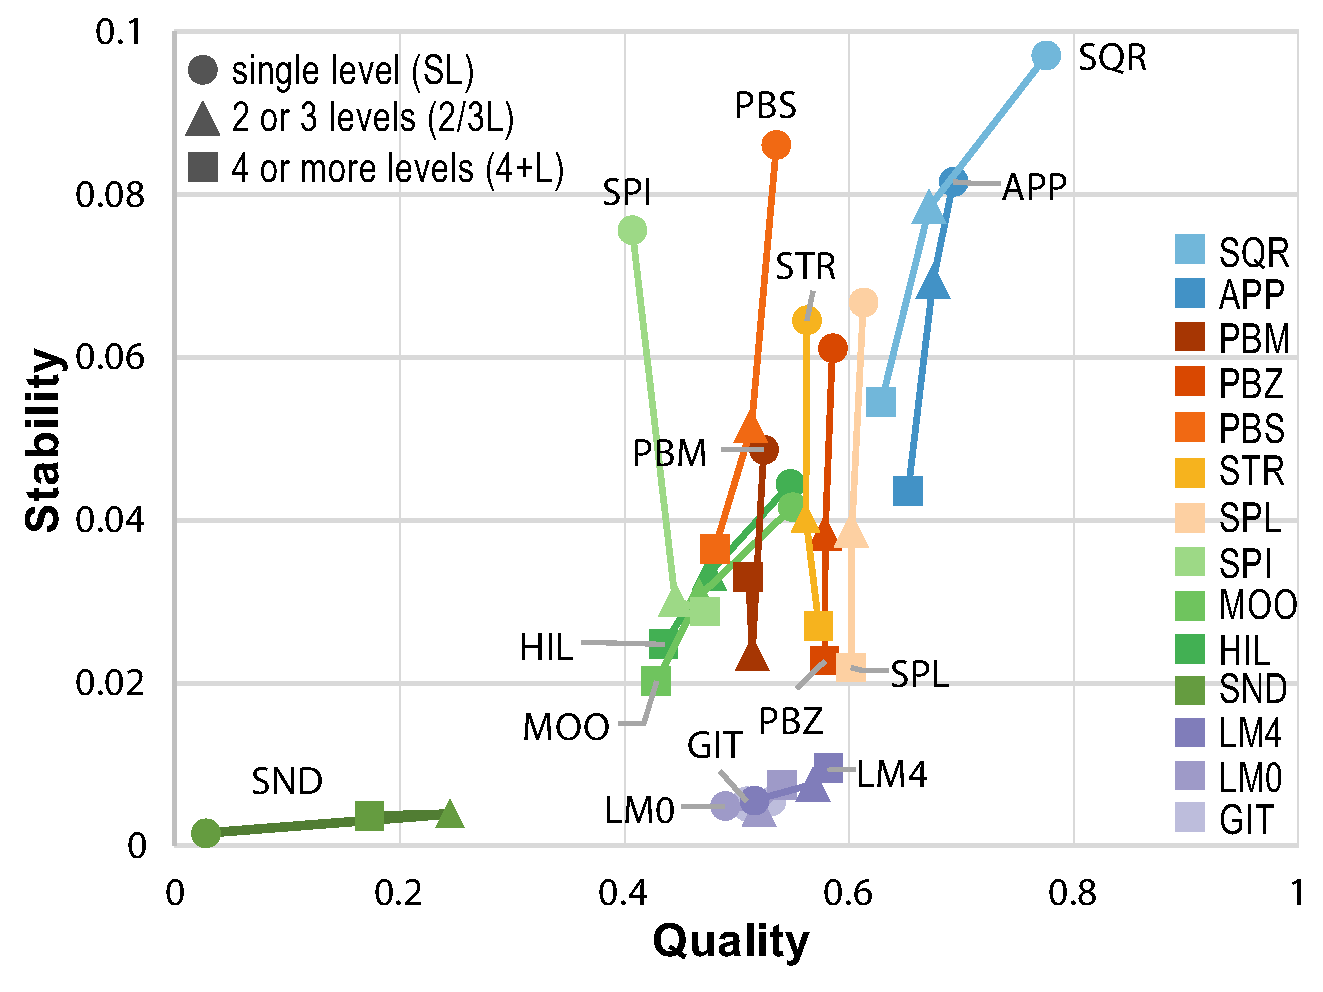
\includegraphics[width=.7\linewidth]{figures/treemap-evaluation/DepthPlot}
    \caption{Visual quality \emph{vs} stability as function of the levels of hierarchy feature.}
    \label{fig:depth}
\end{figure*}

\begin{figure*}[h!]
\centering
    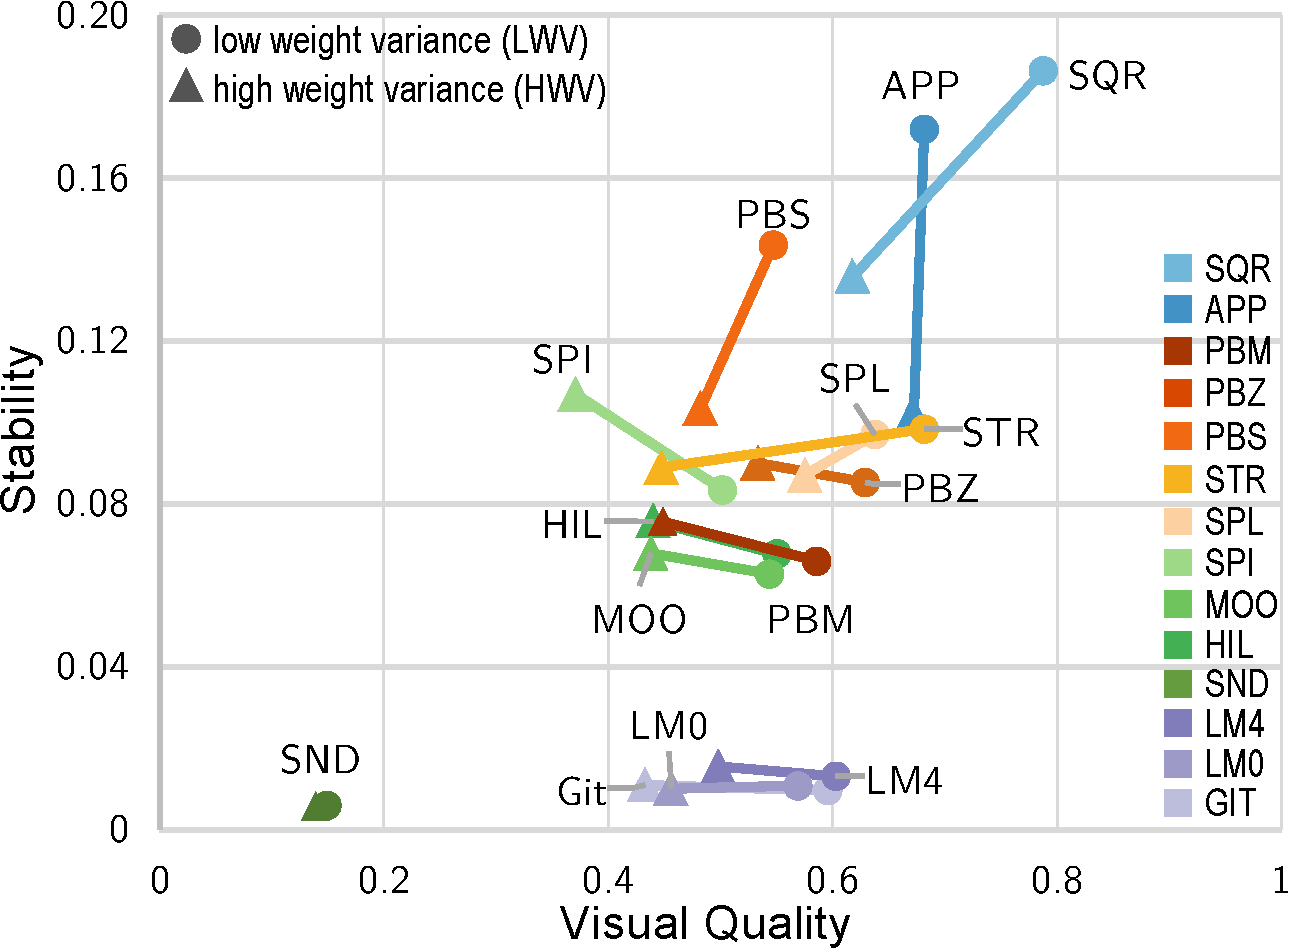
\includegraphics[width=.7\linewidth]{figures/treemap-evaluation/weightVariancePlot}
    \caption{Visual quality \emph{vs} stability as function of the variance of node weights feature.}
    \label{fig:weightVariance}
\end{figure*}

\begin{figure*}[h!]
  \centering
    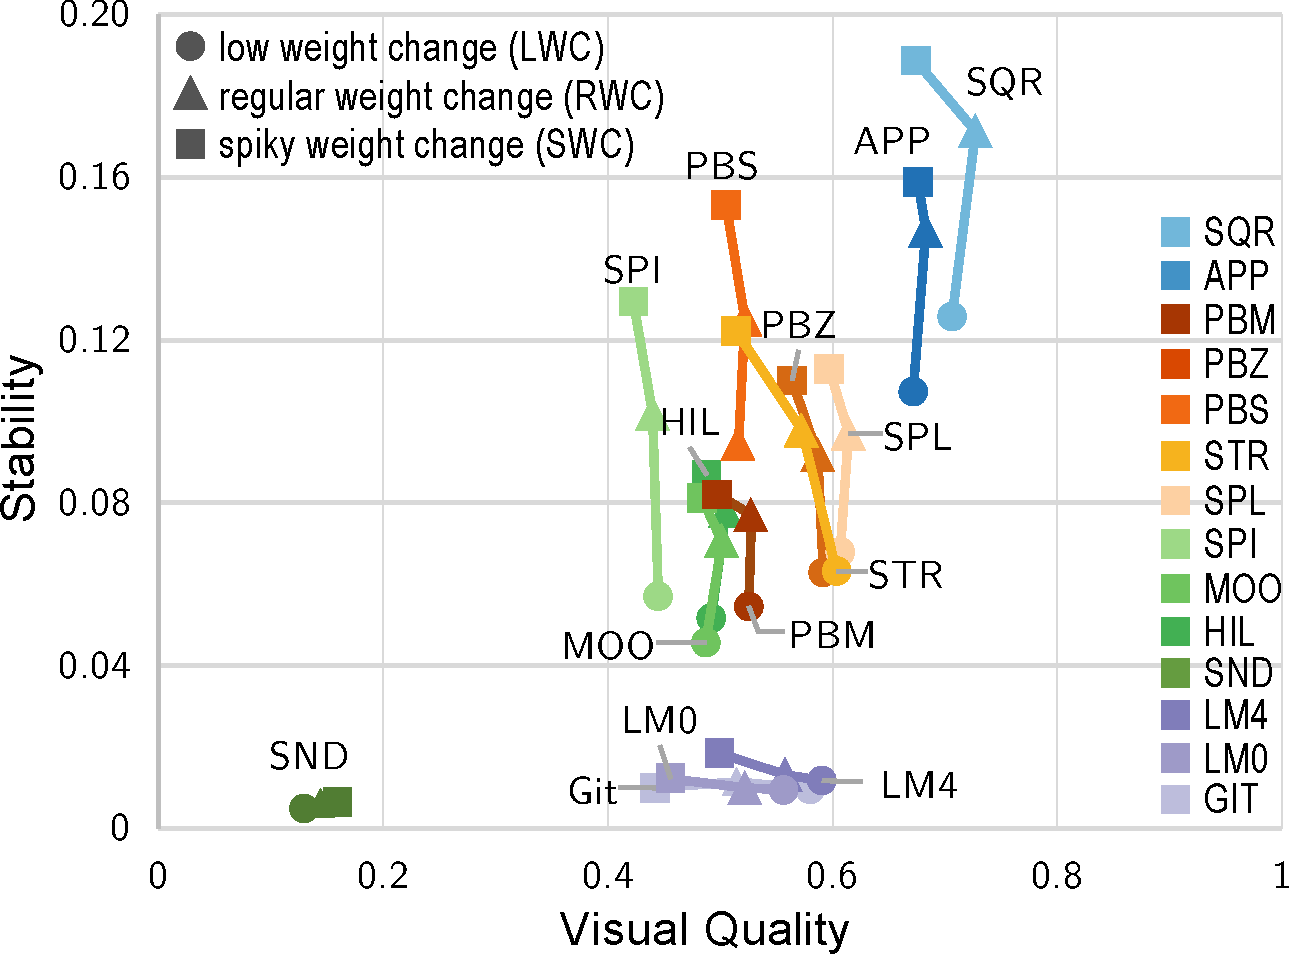
\includegraphics[width=.7\linewidth]{figures/treemap-evaluation/WeightChangePlot}
    \caption{Visual quality \emph{vs} stability as function of the weight change feature.}
    \label{fig:weightChange}
\end{figure*}

\begin{figure*}[h!]
    \centering
    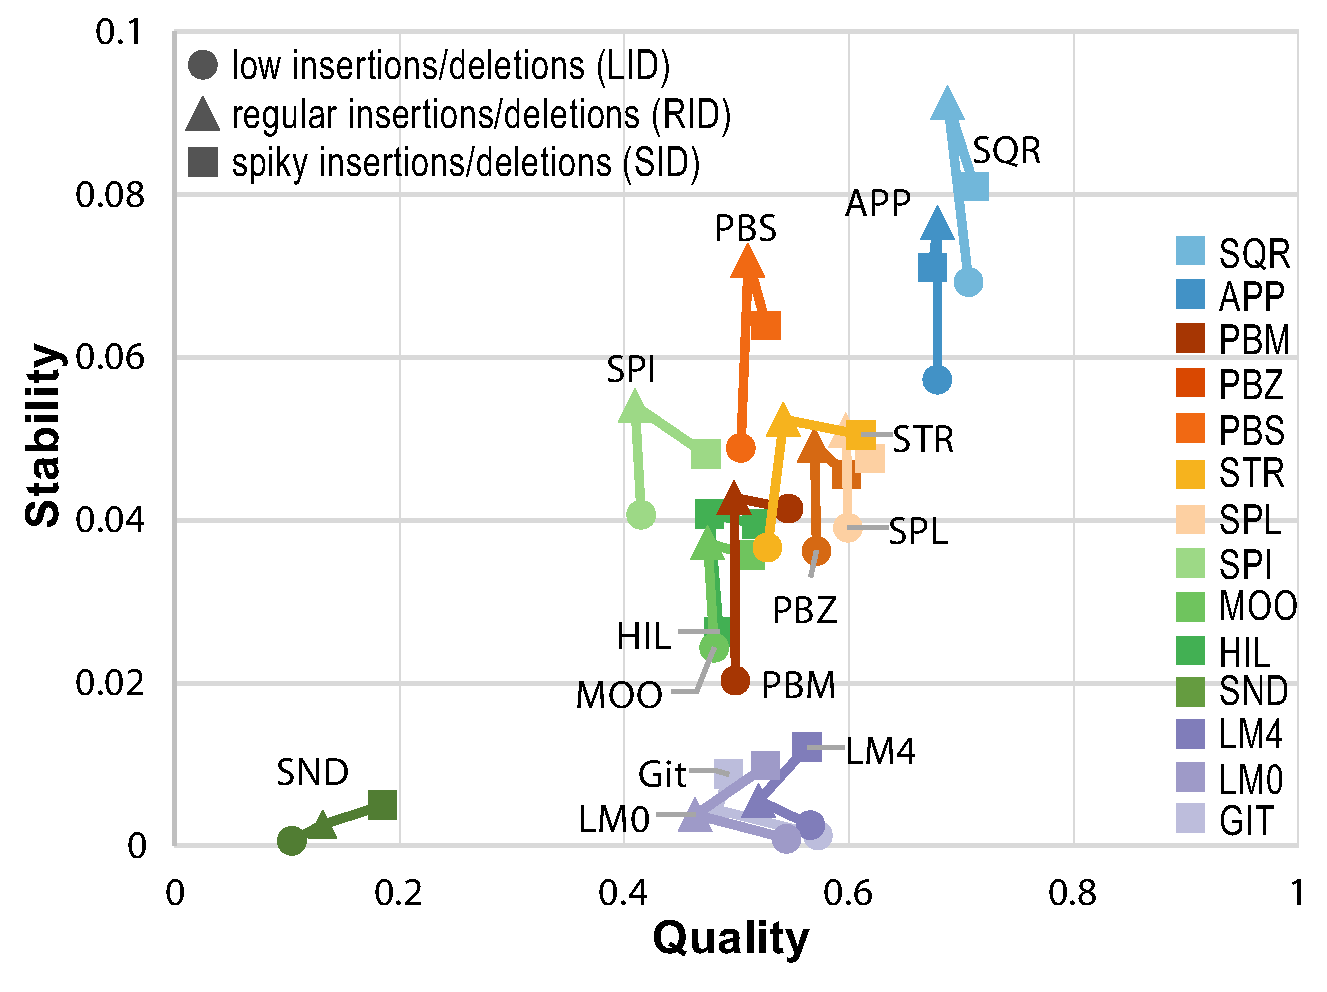
\includegraphics[width=.7\linewidth]{figures/treemap-evaluation/insertionsDeletionsPlot}
    \caption{Visual quality \emph{vs} stability as function of the insertions and deletions feature.}
    \label{fig:insertionsDeletions}
\end{figure*}

%Summarize makes sense? Might want to include, but I don't think it makes sense. Not that much text to read.

%Summarizing the insights obtained from this analysis, we see that
%\begin{itemize}
    %\item SND seems to be the least affected by the considered features, as it is consistently very %stable but of poor visual quality;
    %\item State-aware methods (LM0,LM4,GIT) are little affected by changes in any of the features. %They yield consistently average visual quality and are very stable.
    %\item Unordered methods (SQR,APP) get high visual quality but are very unstable for all feature %values.
    %\item The stability of the remaining methods (ordered, stateless) is strongest affected by the %levels of hierarchy and weight change features; their stability is strongest affected %by the variance of node weights feature.
%\end{itemize}


\subsection{Comparison of data classes}
\label{sec:comparison}
%
We next compare the relative performance of all algorithms separately on all data classes. 
% This information refines the insights obtained in Section~\ref{sec:acrossfeatures} in helping users to choose a suitable algorithm for a given data class. 
\cref{fig:rankingtable-a,fig:rankingtable-b,fig:rankingtable-c} support this comparison as follows: it is structured as a matrix of tables, one per data class.
Each table shows the average visual quality (left column) and average stability (right column) of all algorithms for all datasets in the respective data class. The two columns are sorted separately to show the best-ranking algorithms at the top. Cells show the algorithm names and scores, and are categorically color-coded on the algorithm name, following the same color scheme as in Section~\ref{sec:acrossfeatures}. Empty cells indicate data classes for which we did not find datasets.
\cref{fig:rankingtable-a,fig:rankingtable-b,fig:rankingtable-c} can answer the following practical questions:
%
\begin{description}
\item[Which method is best for my data?] Given a family of datasets with known characteristics (feature values), we search for the corresponding cell and pick the top algorithm(s) in visual quality, stability, or a combination of both, depending on the application requirements. When doing this, we should examine the actual values, since several algorithms score quite close to each other.
\item[How is a given algorithm performing in general?] We scan the table following the color of the respective algorithm, and detect its rank (with respect to visual quality and/or stability) over all data classes. In this way we can find patterns and outliers in the data for this algorithm: for example, LM0 and LM4 are always near the top in stability, and GIT's performance on visual quality fluctuates widely depending on the data class.
\item[Which algorithms perform similarly?] We locate groups of neigh\-boring rows with the same color pattern in all tables. These indicate algorithms which score similarly regardless of data class.
\end{description}
%
%We can read Figure~\cref{fig:rankingtable-a,fig:rankingtable-b,fig:rankingtable-c} in several ways. 

There are a number of additional insights we can obtain from \cref{fig:rankingtable-a,fig:rankingtable-b,fig:rankingtable-c}. When we consider only the visual quality, we see that SQR is usually the best for low-weight variance data, but for high weight variance APP is just as often the best algorithm. If the dataset contains only 1 level, SQR performs better, but for the other depth subclasses it depends on the exact data class.
%
If only the stability is important, SND almost always scores best regardless of the data class, but likewise it consistently scores the poorest on visual quality. 
The state-aware algorithms all perform very well on stability. While LM0 is better in terms of stability than LM4, their exact order as well as their relative order to GIT varies depending on the data class.
%
When considering which algorithm is best for both stability and visual quality, there are no easy answers. There is no algorithm that performs best on both in any of the data classes and hence the answer depends on the desired trade-off and the data class in question.



%\begin{figure*}[htbp!]
%\centering
%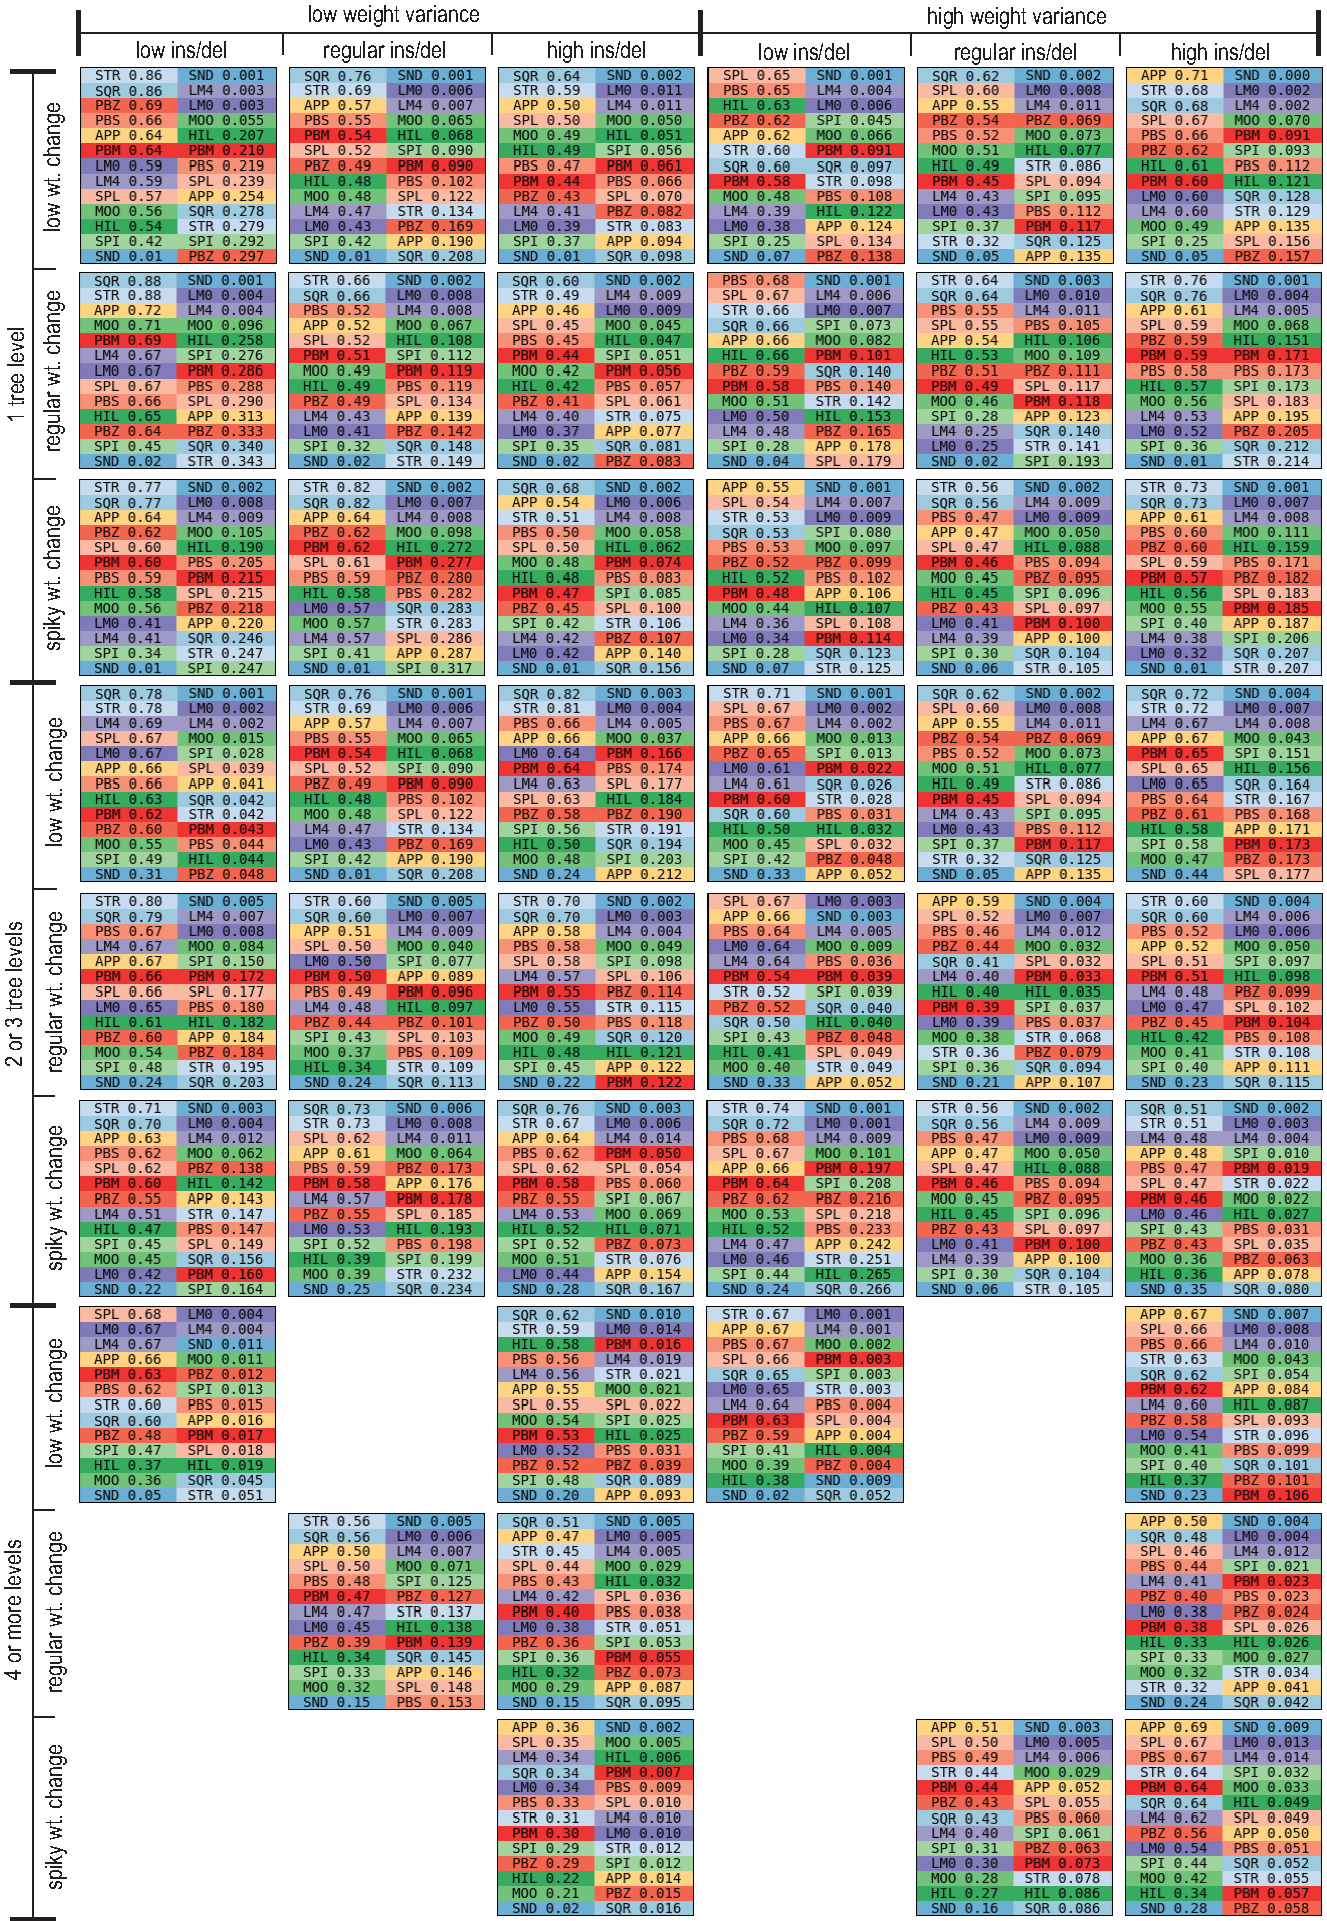
\includegraphics[width=\linewidth]{figures/treemap-evaluation/rankingtable.png}
%\caption{Relative ranking of treemapping algorithms for all data classes. Each table cell shows algorithms in top-down decreasing order of average visual quality (left column) and average stability (right column).}
%\label{fig:rankingtable-a,fig:rankingtable-b,fig:rankingtable-c}
%\end{figure*}

\begin{sidewaysfigure}
% \begin{figure*}[]
\centering
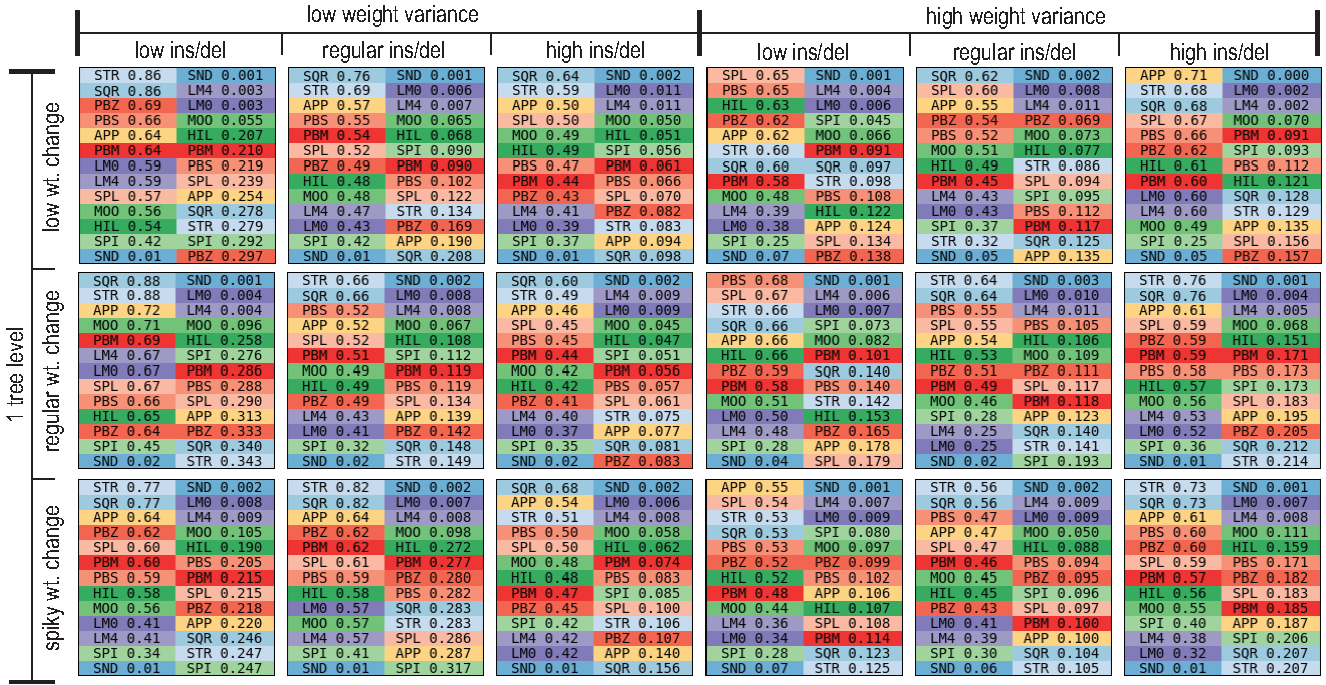
\includegraphics[width=\linewidth]{figures/treemap-evaluation/table-a.png}
\caption{Relative ranking of treemapping algorithms for all data classes. Each table cell shows algorithms in top-down decreasing order of average visual quality (left column) and average stability (right column).}
\label{fig:rankingtable-a}
% \end{figure*}
\end{sidewaysfigure}

\begin{sidewaysfigure}
% \begin{figure*}[]
\centering
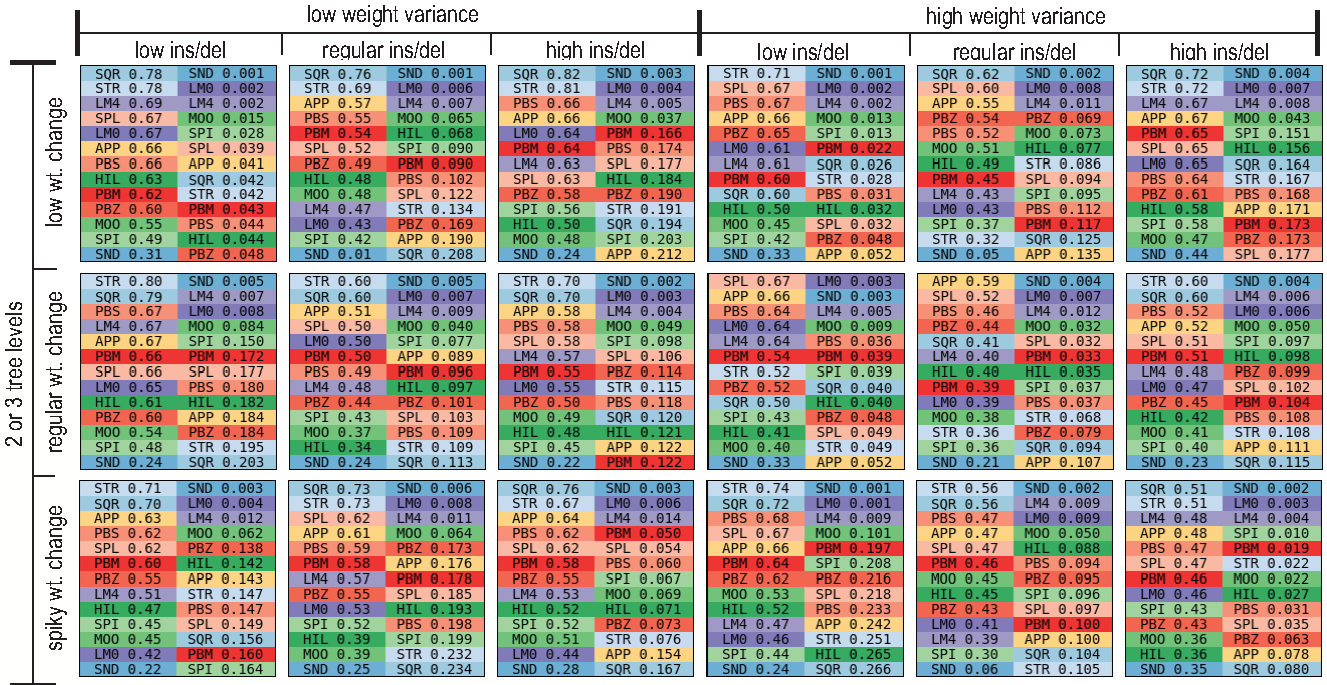
\includegraphics[width=\linewidth]{figures/treemap-evaluation/table-b.png}
\caption{Relative ranking of treemapping algorithms for all data classes. Each table cell shows algorithms in top-down decreasing order of average visual quality (left column) and average stability (right column).}
\label{fig:rankingtable-b}
% \end{figure*}
\end{sidewaysfigure}

\begin{sidewaysfigure}
% \begin{figure*}[]
\centering
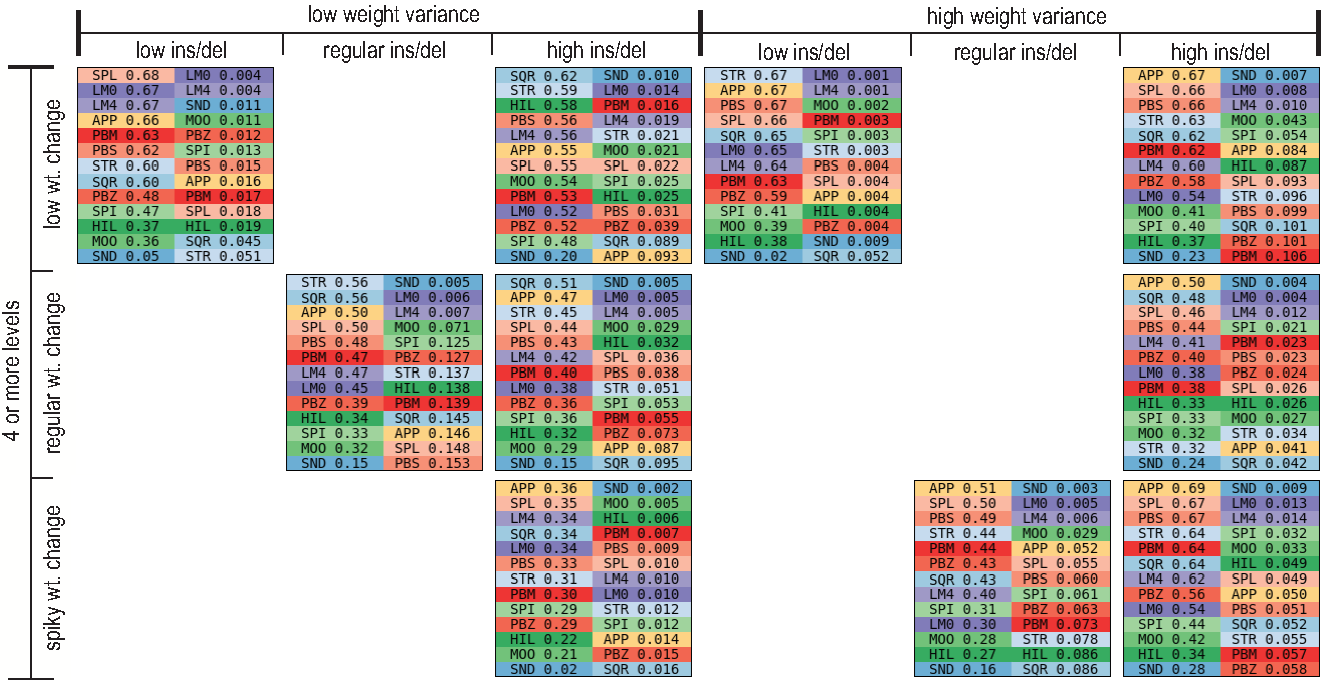
\includegraphics[width=\linewidth]{figures/treemap-evaluation/table-c.png}
\caption{Relative ranking of treemapping algorithms for all data classes. Each table cell shows algorithms in top-down decreasing order of average visual quality (left column) and average stability (right column).}
\label{fig:rankingtable-c}
% \end{figure*}
\end{sidewaysfigure}


\section{Discussion and Conclusion}
\label{sec:discussion-2}

We performed an extensive quantitative evaluation of rectangular treemaps for time-dependent data. To do so, we introduced a new methodology based on baseline treemaps to measure the stability of time-dependent treemaps. Baseline treemaps enable us to measure the change in the input data in a manner that is mathematically comparable to the measures for the layout change of the corresponding treemaps. Furthermore, we proposed a novel classification scheme for time-dependent data sets via a four-dimensional feature space (weight variance, weight change, tree depth, and the pattern of insertions and deletions). These four features naturally arose from a discussion on various types of state-of-the-art treemapping algorithms. Our experimental analysis shows that our proposed classification is valid in general and that most data classes are well suited to predict the performance of treemapping algorithms. For most data classes, our visual summary comparing all algorithms across all data classes and both metrics can hence serve as a reliable resource for researchers and practitioners. Last but not least, all datasets, metrics, and algorithms used in our evaluation are openly available~\citep{URLTreemaps}.

\mypar{Limitations and future work} Our experiments show that our identified features and the resulting feature space generally work well and result in a meaningful classification of datasets. However, there are whole sets of data classes for which we could not find sufficiently many (or even any) datasets. This is partially inherent in the classification and somewhat natural: data sets with low weight variance hardly ever exhibit spiky weight change behavior, so that particular column in our table is essentially empty. But among the 18 classes of treemaps with 4 or more levels we found a significant number of datasets only for two classes, which both are essentially populated by datasets stemming from software repositories. The question remains if there are other significant types of time-dependent hierarchical datasets which have four or more levels and which escaped our searches. As it is, the results for these two particular classes are representative for only a restricted type of data.

Our classification works well for visual quality, with the exception of two cases (2/3 level, spiky insertions and deletions, high weight variance, and low or spiky weight change). We have a large number and variety of datasets at our disposal for these two classes, but nevertheless, it is unclear to us what causes these inconsistencies in the performance of the tested algorithms. There might be a hidden correlation in these datasets and one or more additional features might be needed to separate these classes further.

While we do have a significant number of datasets at our disposal and hence can validate our claims with some certainty, we still might be observing some bias in our collection. As stated above, essentially all datasets with 4 or more levels stem from software repositories. Furthermore, all World Bank datasets have at most 3 levels. It would be interesting to analyze if and how this bias in the data influences our results.
To overcome possible data bias, we would also like to construct, and evaluate on, synthetic datasets. Doing so is not trivial; creating datasets that avoid sampling biases and are representative of real-world datasets (for a suitable definition of ``real-world'') is a challenging (but important) question in its own right in information visualization in particular and in data science in general.

To complement our quantitative evaluation it would naturally be of interest to evaluate the performance of treemapping algorithms in various usage scenarios through user studies. The two metrics we use for visual quality and stability are both perceptually salient according to studies performed in previous work. However, a study that evaluates the combination of and the trade-offs between visual quality and stability could deliver important insights as to where on the Pareto-front an optimal treemapping algorithm should lie.

Finally, our evaluation currently does not measure the run-time and correspondingly the computational scalability of the algorithms used in our experiments. Our implementations are not (equally) optimized and hence a fair comparison is currently risky if not impossible. Scalability is clearly an important factor in online usage scenarios, and we hope to be able to complement our current set of implementations with optimized versions in the near future.


\chapter{Treemap Algorithm}

% https://github.com/EduardoVernier/git-latex
% A Stable Greedy Insertion Treemap Algorithm for Software Evolution Visualization

\section{Introduction} \label{sec:intro}
%
%
Understanding the evolution of large and long-lasting software projects is a major aspect of program comprehension. Typically, evolution data for such projects is mined by fact extraction tools from existing software control management systems handing software repositories, such as Git\cite{git}, Subversion\cite{subversion}, and CVS\cite{cvs}.
% I'm not sure how to cite these Source Control Managers, so I'm just linking to their official webpage.
Several types of data attributes are collected (and explored) in this way, including the identity of software items of interest (\emph{e.g.}, packages, folders, files, classes, methods), various quality attributes measured on them (\emph{e.g.}, testability, maintainability, modularity, and readability metrics~\cite{lanza06}), and relations that interrelate these items. \emph{Hierarchy} relations, which describe the containment or aggregation of software items, play a central role in virtually all such evolution analyses, since they offer a powerful and natural way to examine the (typically large) evolution data at multiple levels of detail. As such, methods that can depict time-dependent hierarchies are a central element of the program evolution toolset.

Dynamic, or time-dependent, treemaps are one of the most effective techniques for displaying time-dependent hierarchies. Compared to other techniques, such as node-link tree layouts, they use basically every pixel of the available screen space to display information, and as such scale to tens of thousands of items (tree nodes) per time step. Many treemap methods exist for handling static (time-independent) hierarchies~\cite{shneiderman92,sqr}, which also have been shown to optimize various quality measures that help readability, such as aspect ratio~\cite{sqr, nagamochi07} and relative positions of nodes~\cite{sot,ordered,Ghoniem2015, Buchin2011,nmap}. However, far fewer methods are available for dynamic trees~\cite{hahn10,sondag17,htm}. One key problem for dynamic treemapping is \emph{instability}, \emph{i.e.}, the fact that relatively small changes in a tree can induce disproportionately large changes in the resulting treemaps. Finding a good way to quantify and reduce instability is an open problem for dynamic treemap algorithms.

In this paper, we address the above limitations with two main contributions. Firstly, we propose a new dynamic treemap algorithm, called Greedy Insertion Treemap (GIT). GIT aims to preserve treemap-cell neighborhoods over time by constructing an initial so-called Layout Tree (LT), which is next incrementally updated as the tree data changes, so as to minimize undesired treemap-layout changes.
Secondly, we evaluate the quality of GIT both in the spatial domain and the temporal domain against a large set of well-known treemap algorithms using several established quality metrics, and on a large set of dynamic hierarchies extracted from real-world software repositories. Our evaluation results show that GIT strikes a better balance between spatial and temporal quality than the existing competing methods we evaluated against. As GIT has a simple and computationally scalable implementation, we argue that it represents a valuable contribution to the toolset of techniques needed by program evolution comprehension.

The structure of this paper is as follows. Section~\ref{sec:related_work} outlines existing work on (dynamic) treemapping and related quality metrics, and their use in program evolution comprehension, and also introduces the treemap methods we compare against. Section~\ref{sec:git} details our new GIT algorithm. Section~\ref{sec:evaluation} presents our evaluation methodology for GIT and the obtained results are revealed in Section~\ref{sec:results-3} . Section~\ref{sec:conclusion-3} discusses our proposal and outlines directions for future improvement.


\section{Related Work}
\label{sec:related_work}

In this section, we will discuss the Algorithms (Section~\ref{sec:algorithms}) and Quality Metrics (Section~\ref{sec:metrics-3}) present in the dynamic treemap literature.
Let $T= \{n_i\}$ be a hierarchy (tree) with nodes $n_i$, each having a weight value $a_i \geq 0$. Weights are given for leaf nodes and computed for non-leaf nodes as the sum of their children weights, respectively. Let ${\cal T}(T)$ be the treemap layout of $T$, with a rectangle cell $r_i$ assigned to each $n_i$, so that the area of $r_i$ equals $a_i$.

\subsection{Algorithms}
\label{sec:algorithms}
%
Time-dependent hierarchies $T(t)$ are a central artifact to explore in program evolution comprehension. Since such analyses usually involve tens or even hundreds of time steps $t$, small-multiple visualizations (one image per time step) do not scale well, hence showing an animated layout of the changing hierarchy is preferred~\cite{diehl08}. For this, several techniques construct a so-called union tree $\cup_tT(t)$, build a single layout of this union tree, display it using Icicle plots~\cite{Kruskal1983} or Sunburst diagrams~\cite{sunburst}, and then highlight changes of $T(t)$ over time in it~\cite{ersoy_sequence}. While this approach minimizes instability (layout changes) over time, and is simple to implement, it cannot handle long time sequences and/or large trees.

Treemaps cope well with the need for handling large trees~\cite{schulz11_treesurvey,hci_treemaps,treevis,landesberger11}.  Slice and dice (SND) treemaps introduced the idea but were found to create poor aspect-ratio (AR) cells which are hard to see\,\cite{shneiderman92}. Squarified treemaps (SQR) propose a heuristic that yields good (close to one) AR values\,\cite{sqr}. A subsequent algorithm (APP) was designed to approximate the optimal AR\,\cite{nagamochi07}. While treemaps were originally designed to handle time-independent trees, the need for \emph{stability} was soon revealed -- that is, small changes in the input tree $T$ should yield only small changes in the treemap ${\cal T}(T)$.
Several algorithms were designed to improve stability. Ordered treemaps (OT)~\cite{ordered} and Strip treemaps (STR)~\cite{bederson02} lay out cells $r_i$ using a given order of the nodes of $T$, using different heuristics -- Pivot-by-Middle (PBM), Pivot-by-Size (PBZ), and Pivot-By-Split-Size (PBS)~\cite{ordered}. Other algorithms lay out cells along a space-filling fractal-like curve, \emph{e.g.}, Spiral (SPI)~\cite{spiral}, and Hilbert (HIL) and Moore (MOO) methods~\cite{hilbert_moore}. Yet another ordering technique considers node similarities: Spatially-Ordered Treemaps (SOT)~\cite{sot} processes sibling nodes ordered by decreasing similarity; NMap~\cite{nmap} places cells according to the similarity of their nodes using dimensionality reduction. Variants thereof include NMap Alternate Cuts (NAC), which splits the screen space alternating horizontal and vertical slices; and NMap Equal Weights (NEW) which aims to create similar-size cells.

Stability becomes a major concern when treemapping time-independent trees with potentially long evolution and large variations. However, only a few methods explicitly aim to treat dynamic data. Stable treemaps~\cite{sondag17} aim to improve both AR and stability by using non-sliceable layouts. However, this method is computationally expensive and not trivial to implement. Voronoi treemaps~\cite{balzer05,balzer05b}
achieve, in general, good AR values, and have been adapted to also handle dynamic trees to visualize software structure evolution~\cite{hees17,gotz11}. There exist also methods that propose other cell shapes, or combinations of multiple shapes, such as bubble treemaps~\cite{bubble}, jigsaw treemaps~\cite{jigsaw}, and orthoconvex treemaps~\cite{deberg14}. However, such methods have not been specifically designed with the aim of maximizing stability.
% I believe hybrid was, so I removed it from this list: hybrid treemaps~\cite{htm}


\subsection{Metrics}
\label{sec:metrics-3}
%
As outlined in Sec.~\ref{sec:algorithms}, treemap quality consists of two main components:

\emph{Spatial} quality captures how readable the treemap geometry is. The best known, and most used, metric for this is the aspect ratio (AR) of the cells $r_i$ which should ideally reach one. The so-called readability metric measures how often a user's gaze changes direction while reading an ordered treemap along the predefined node ordering~\cite{bederson02}. The continuity metric measures how often cells of nodes which are close in the given node ordering are far apart in the treemap~\cite{spiral}. % A very similar concept is used to quantify the quality of dimensionality reduction methods~\cite{lamp,martins}. Couldn't find the references...

\noindent\emph{Stability} metrics capture how easily can a user understand the changing geometry of a dynamic treemap. This is measured essentially by quantifying the visual change $\delta(r_i(t), r_i(t+1))$ of the cells $r_i$, and then aggregating such visual changes into a single value using some function $S$. Early on, Shneiderman and Wattenberg~\cite{ordered} defined the Layout Distance Change metric, where they used for $\delta$ the distance between the vectors $(x_i(t), y_i(t), w_i(t), h_i(t))$ and $(x_i(t+1), y_i(t+1), w_i(t+1), h_i(t+1))$, $x$ and $y$ being the coordinates of the top-left corner, and $w$ and $h$, the width, and the height of a rectangle $r_i$. They defined $S$ as the average of $\delta$ for all cells and revisions. Later, Hahn \emph{et al.}~\cite{hahn10} use for $\delta$ the distance between the centers of $r_i(t)$ and $r_i(t+1)$ and also average for $S$. Tak and Cockburn~\cite{hilbert_moore} use for $S$ the variance and define $\delta$ as~\cite{ordered}. They also propose a drift metric, which measures how much a cell's center moves away from its average position over long time intervals. Recently, we have seen new metrics that measure stability not by looking only at a single cell's position relative to its past states, but take into consideration the relationships between all cells in the layout. Hahn et al.~\cite{Hahn2017} propose the relative direction change, which measures angle differences between all centroids in the layout between consecutive time-steps, and Sondag \emph{et al.}~\cite{sondag17} propose similar metric, where $\delta$ measures how a cell moves with respect to all its neighbors, where $S$ is again the average.
We will discuss these metrics further, and also propose a new one in Section~\ref{sec:eval_metrics}.

\section{Greedy Insertion Treemap}
\label{sec:git}
%
As outlined in Sec.~\ref{sec:related_work}, many treemapping methods exist in the literature, and these have been evaluated by several metrics for both spatial quality and stability. However, examining the above in more detail, we find two limitations: (a) most existing treemap methods have been designed without the \emph{explicit} aim of maximizing stability; (b) among the few methods where stability was an aim, there is no clear optimal method which yields both good spatial quality and stability for long time sequences of trees exhibiting a high dynamics in terms of node additions, deletions, and weight changes. We next propose a method, Greedy Insertion Treemap (GIT), that aims to outperform the current state-of-the-art in these two respects.


GIT is designed from the start with the aim of increased stability. For this, GIT aims to preserve cell neighborhoods in the treemap over time. To this end, we use a so-called Layout Tree ($LT$) help data structure (not to be confused with the tree $T$ we want to visualize).
Each node $l \in LT$ represents a treemap cell, and may have two subtrees: (a) $R(l)$ is rooted at the top-right corner of $l$; and (b) $B(l)$ is rooted at the bottom-left corner of $l$. Together with the cell weights, $LT$ fully encodes a treemap ${\cal T}$. Indeed, we can construct ${\cal T}$ by traversing $LT$ breadth-first.
During this, for each $l \in LT$, we compute the total weight of its subtrees $R(l)$ and $B(l)$, and cut the remaining drawing space vertically and horizontally according to these summed weights, as illustrated in Fig.~\ref{fig:space-partition}.

\begin{figure}
\centering
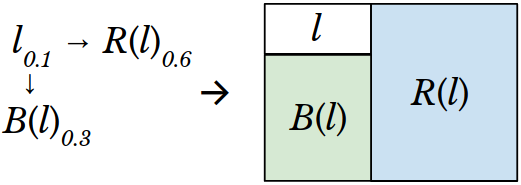
\includegraphics[width=.8\textwidth]{figures/treemap-algorithm/space-partition.png}
\caption{Space partitioning from $LT$.}
\label{fig:space-partition}
\end{figure}

GIT proceeds in two phases: initialization and update, as follows.\\

\noindent\textbf{Initialization:} To start with, we need to construct $LT$ from the first tree $T(t=0)$ in our sequence. For this, we can use basically any method ${\cal T}_{init}$ that constructs a (static) treemap for $T(0)$ from which we can next generate $LT$ with the properties (a) and (b) mentioned above. We have experimented with two such initialization methods. First, we constructed $LT$ from a squarified treemap (\emph{i.e.} ${\cal T}_{init}$ is the SQR algorithm), since SQR is well known to yield very good AR values. Alternatively, we propose a simple heuristic ${\cal T}_{init}^{direct}$ that directly builds $LT$ from the initial tree $T(0)$. Both initialization methods are compared next in Sec.~\ref{sec:results-3}.

To explain our heuristic ${\cal T}_{init}^{direct}$, consider a single-level tree $T = [(n_i,a_i)]  =  [ (A, 10), (B, 2), (C, 8), (D, 4), (E, 1), (F, 3) ]$, to be laid our, for simplicity, in a square drawing area $S$ of size 1; handling general trees is trivial by top-down recursion. We build $LT$ by sequentially adding each $n_i \in T$ to it (Fig.~\ref{fig:git_example}). After each addition, we rebuild ${\cal T}$ from the current $LT$ as explained above, so it covers the entire $S$. Thus, existing nodes are `squeezed' to make space for the new nodes. In our example, we first add node $A$, which will cover the entire $S$. To add $B$, we find the node $n \in LT$ having the worst aspect-ratio cell $c \in {\cal T}$. If $w_c \geq h_c$, we add $B$ directly right of $n$ (as in our example), else we add $B$ directly below $n$, and update ${\cal T}$ from the new $LT$ again. For the third node $C$, as the worst-aspect-ratio cell is $B$, and since $h_B > w_B$, we add $C$ below $B$ and update ${\cal T}$ from $LT$ again. Fig.~\ref{fig:git_example}(d-f) shows the addition of the remaining nodes of $T$.\\

\begin{figure}[htbp!]
\centering
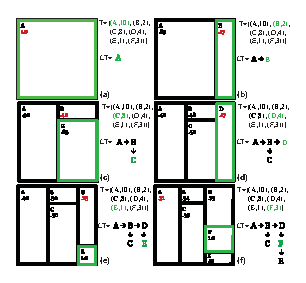
\includegraphics[width=.8\textwidth]{figures/treemap-algorithm/git_example.eps}
\caption{Building the initial layout tree $LT$ (green: inserted cells).}
\label{fig:git_example}
\end{figure}

For didactic purposes, nodes were added in alphabetical order, but in reality, we want nodes to be added in random order, hence when dealing with truly hierarchical data, one sub-tree is not completely laid out before its siblings, which could cause it to be `squeezed'.

\noindent\textbf{Update:} We now have an initial treemap ${\cal T}$ and its $LT$. We next edit $LT$ to handle weight changes, node additions, and node deletions as $T$ changes. \emph{Weight} changes do not change $LT$. \emph{Additions} are handled just as adding regular nodes when building the initial $LT$ using ${\cal T}_{init}^{direct}$. Additions tend to increase the cells' aspect ratios, so we do them after node removals and weight changes. \emph{Removals} are done by editing $LT$ as follows (see also Fig.~\ref{fig:git_removal}):

\begin{enumerate}
\item If a node $n\in LT$ has a $B(n)$ subtree, we replace $n$ by $B(n)$;
\item else if $n$ has a $R(n)$ subtree, we replace $n$ by $R(n)$;
\item else $n$ has no subtrees, so we just remove it from $LT$.
\end{enumerate}

After handling all changes in a new revision of $T$, we rebuild ${\cal T}$ from $LT$, as already explained. As we show next in Sec.~\ref{sec:results-3}, GIT scores a very good balance of spatial quality \emph{vs} stability.

\begin{figure}[htbp!]
\centering
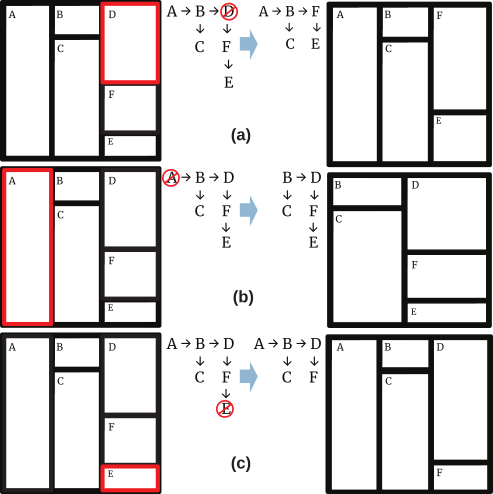
\includegraphics[width=.8\textwidth]{figures/treemap-algorithm/git_removal.eps}
\caption{Removal of nodes (red) from layout tree and its treemap.}
\label{fig:git_removal}
\end{figure}


\section{Evaluation}
\label{sec:evaluation}
%
To evaluate GIT, we considered the following aspects:

\subsection{Metrics}
\label{sec:eval_metrics}
%
To evaluate the quality of GIT, we proceed as follows. For spatial quality, we use the well-known Aspect Ratio metric ($AR$)~\cite{sqr}. For each cell $c$ in a treemap ${\cal T}$, $AR_c = min(w_c, h_c)/max(w_c, h_c)$. This metric is considered by virtually all rectangular treemap evaluations we are aware of.

For stability, we compute three metrics. The first two are the Shneiderman-Wattenberg's Layout Distance Change ($LDC$)~\cite{ordered} and Tak-Cockburn's Location Drift ($LD$)~\cite{hilbert_moore}, already introduced in
Sec.~\ref{sec:related_work}. The $LDC$ metric captures the instability of a cell between consecutive revisions. In contrast, the $LD$ metric captures the deviation of a cell's position over all timesteps.

We also propose a (new) third metric, which extends $LDC$ to also consider the change of the \emph{data}. We define the \emph{visual change} of a cell $c_i$ as the Euclidean distance traveled by the four corners of the rectangle $r_i$ between $t$ and $t+1$, normalized by the treemap diagonal $\sqrt{W^2+H^2}$, so $\delta v_i \in [0,1]$. Next, we define the \emph{data change} of $c_i$ as $\delta a_i = |a_i(t)-a_i(t+1)|$, where $a_i$ is the relative weight of node $c_i$. With these, we define the stability $Q_i$ of a cell $c_i$ in a treemap as

\begin{equation}
Q_i =  (1-\delta v_i) / (1 - \delta a_i).
\label{eqn:stab_ratio}
\end{equation}

We define the stability $Q$ of an entire treemap as the average of its cells' stabilities $Q_i$. In contrast to $LDC$, $Q$ measures how much a rectangle changes \emph{in relation to its data change}. Measuring only absolute changes of rectangles ($LDC$) does not, we believe, fully characterize stability. Indeed, a rectangle could (and should) change a lot if its underlying cell's weight changes a lot. However, this does not mean necessarily that the treemap algorithm is unstable.

\subsection{Techniques}
%
We tested GIT against 14 other treemapping algorithms: Approximate (APP), Hilbert (HIL), Stable treemaps (LM0, LM4), Moore (MOO), NMap-Alternate-Cuts (NAC), NMap-Equal-Weights (NEW), Pivot-by-Middle (PBM), Pivot-by-Size (PBZ), Pivot-by-Split-Size (PBS), Slice- and-Dice (SND), Spiral (SPI), Squarified (SQR), and Strip (STR). For NMap, we use as seed layout the one computed by SQR~\cite{nmap}. We did not consider non-rectangular treemap methods in the evaluation, since not all the metrics in Sec.~\ref{sec:metrics-3} directly generalize to non-rectangular cells.

\subsection{Datasets}
%
We extracted 28 dynamic hierarchies by mining the structure of software projects (folders, files, classes) from 28 corresponding public GitHub repositories, using a custom automated pipeline that scans all available revisions and extracts the code structure using Understand~\cite{understand}. As weights $w_i$, we use the number of lines of code of the respective items. Other software quality metrics delivered by Understand can be used instead, if desired. For more details on this process, we refer to~\cite{vmv}. The considered repositories have quite different sizes, number of revisions, hierarchy depths and shapes, number of developers, and code type (programming languages and application types). Statistics about the datasets are available in Table~\ref{tab:datasets-3}.

\begin{table}[htbp!]
\small
\centering
\scalebox{0.9}{
\begin{tabular}{|l|l|r|r|}
\hline
\textbf{Dataset} & \textbf{Revisions} & \textbf{Nodes (total)} & \textbf{Average depth} \\
\hline
animate.css & 50 & 3454 & 2.87\\
AudioKit & 22 & 11178 & 6.95\\
bdb & 62 & 2658  & 3.83\\
beets & 106   & 9844 & 3.75\\
brackets &  88  & 120292 & 12.85\\
caffe & 44 & 12969   & 4.93\\
calcuta & 50 & 2882 & 10.76\\
cpython   & 321 & 584821 & 6.50\\
earthdata-search   &  46& 18539 & 6.82\\
emcee & 64 & 1746  & 3.62\\
exo & 97 &  36436  & 11.88\\
fsharp   & 69 & 22906 & 7.89\\
gimp   & 72 &  170418 & 5.19\\
hospitalrun-frontend   & 38 &  16759 & 5.71\\
Hystrix & 61 & 15530  & 13.29\\
iina & 74 &  6849  & 4\\
jenkins & 137  & 277185 & 11.94 \\
Leaflet &  84  & 13381 & 4.86 \\
OptiKey   & 36 & 9782 & 6.72\\
osquery  & 37 & 14111 & 5.75 \\
PhysicsJS   & 20 & 2022 & 4.6\\
pybuilder   & 53 & 5457 & 7\\
scikitlearn   & 88 & 48468 & 5.75\\
shellcheck   & 53 & 746 & 2.39\\
soundnode-app   & 35 & 3196 & 6.88\\
spacemacs   & 51 & 10201 & 4.96\\
standard   & 29 & 203 & 2\\
uws & 122 & 4093 & 2.76\\
\hline
\hline
\textbf{Totals:} & 2132 & 1458036 & 5.77\\
\hline
\end{tabular}
}
\caption{Software evolution tree datasets used in the evaluation.}
\label{tab:datasets-3}
\end{table}


\section{Results}
\label{sec:results-3}
%
We evaluate GIT on the aforementioned datasets, algorithms, and metrics collection from several perspectives, by answering a series of questions. Below, average stability $S$ refers to the average of the $LDC$ and $Q$ metrics introduced in Sec.~\ref{sec:metrics-3}. All results that we were not able to fit in the paper can be found at our online repository\cite{git-benchmark}.

\subsection{How does GIT's initialization affect its quality?}
%
As outlined in Sec.~\ref{sec:git}, we can initialize GIT with various treemap layouts, such as squarified (SQR) or using the direct initialization illustrated in Fig.~\ref{fig:git_example}. Intuitively, one would think that SQR initialization is to be preferred, since SQR is well known for its high $AR$ values. To test this, we ran GIT using both initializations for all datasets. After initialization, the same regular GIT update mechanism is used in both cases. Figure~\ref{fig:git_vs_sqr} shows the per-dataset average stability and $AR$ values. Interestingly, we see that the higher-$AR$ SQR initialization actually yields slightly worse $AR$ values for the entire sequence. For stability, the two initializations behave basically identically. We can explain this result by the fact that the GIT direct initialization follows the same heuristics as the update steps, while SQR forces GIT to start with a layout which needs more substantial updates next as the tree data changes. At a higher level, this experiment suggests that GIT performs very well using direct initialization. As such, we use this initialization in all subsequent experiments.

\begin{figure}[htbp!]
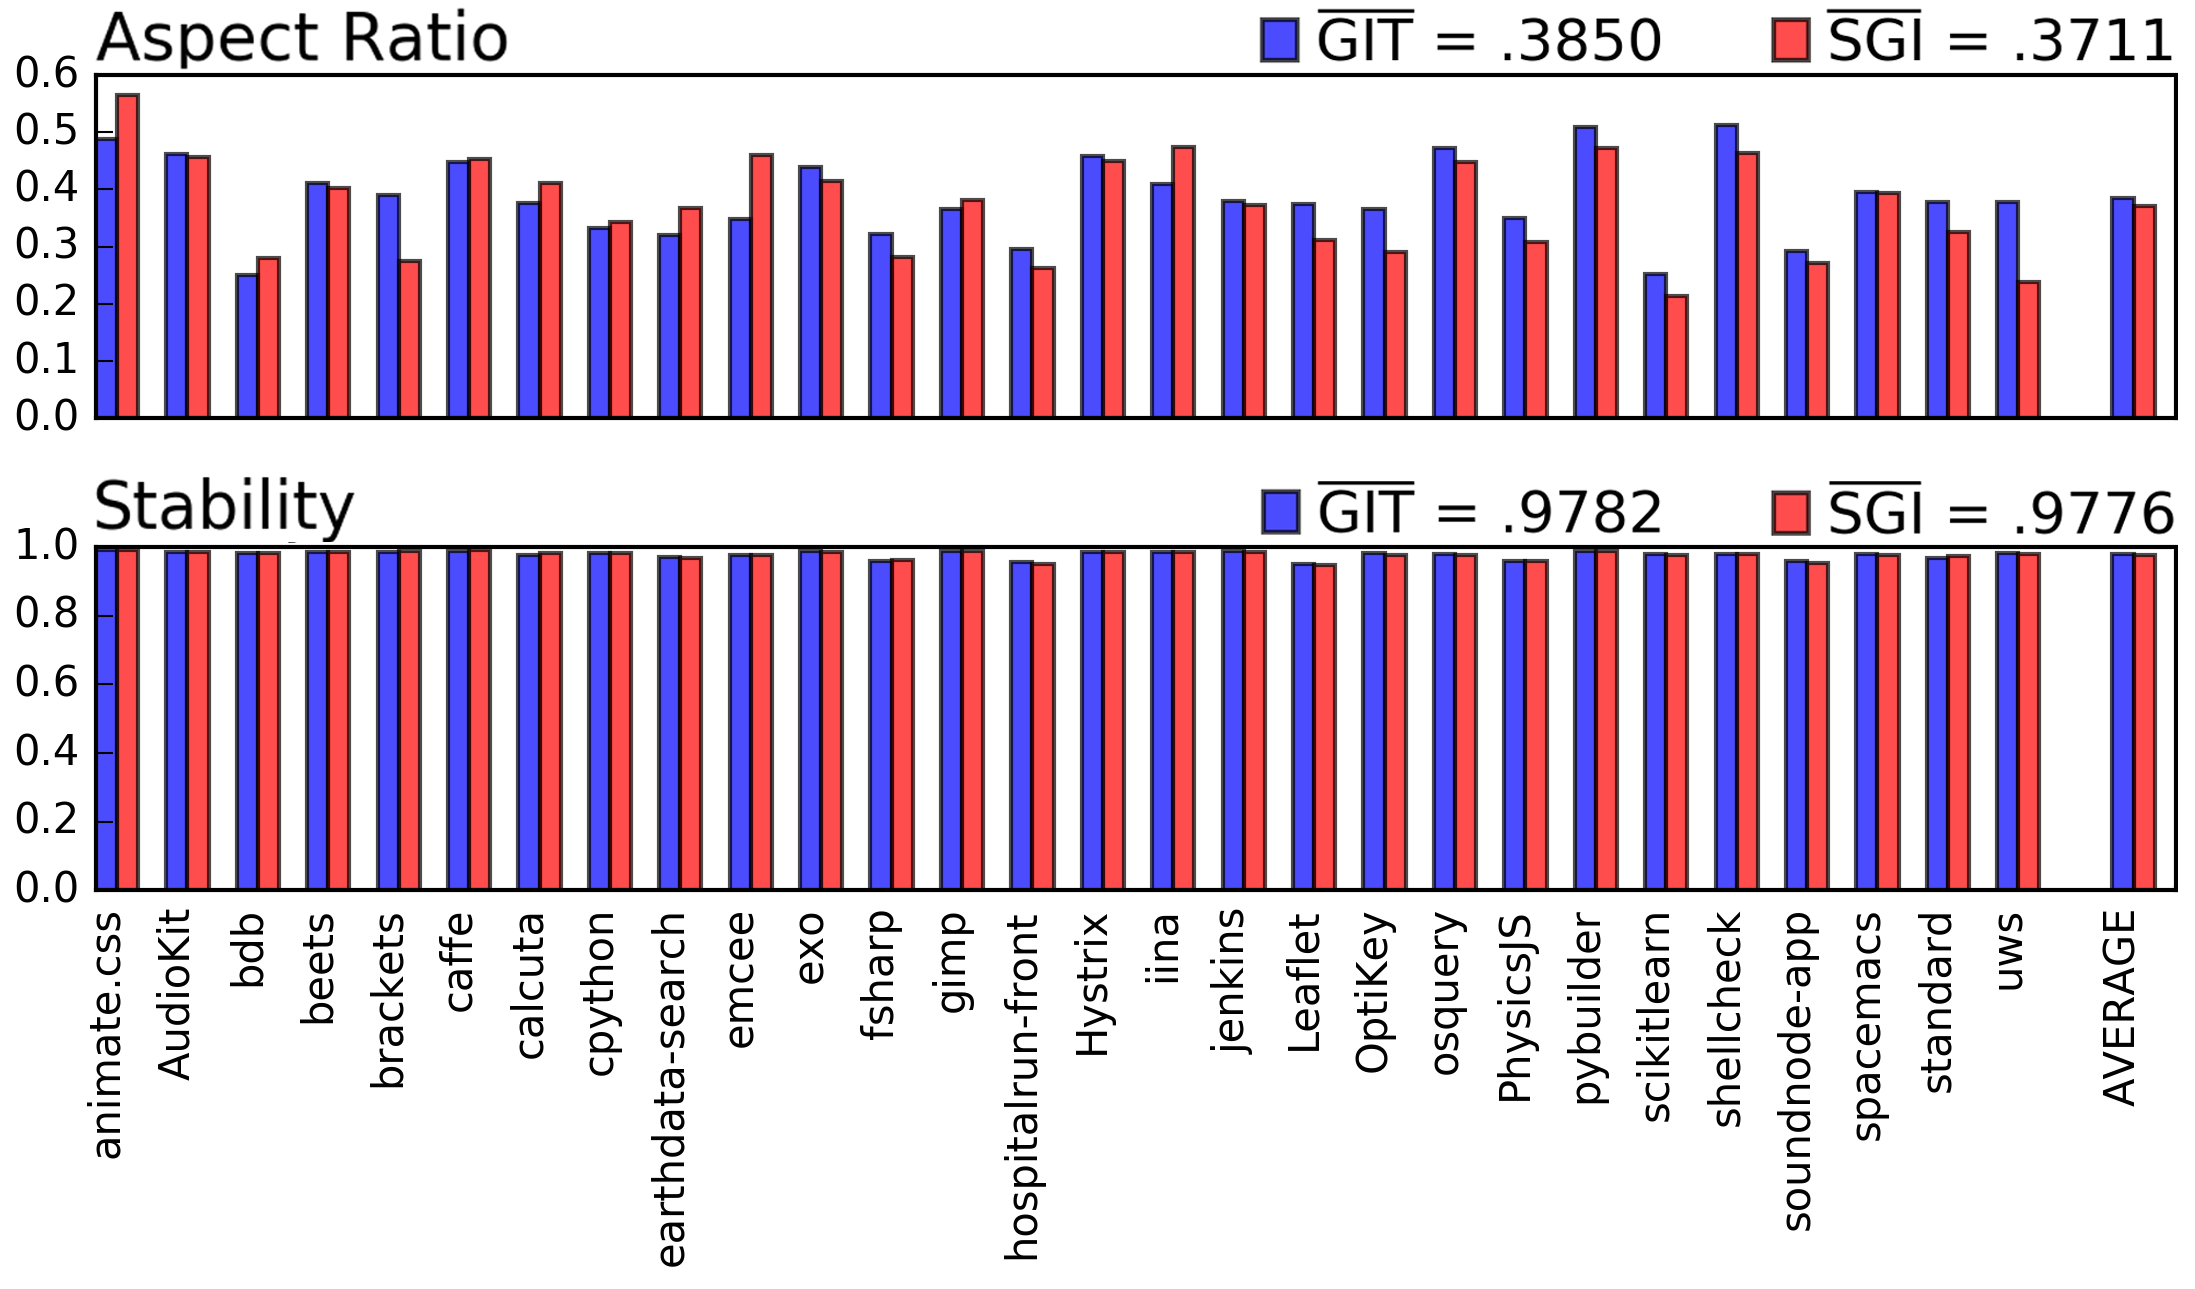
\includegraphics[width=\textwidth]{figures/treemap-algorithm/git-vs-sqrgit-both.png}
\caption{GIT performance using ${\cal T}_{init}^{direct}$ (GIT) \emph{vs} squarified initialization (SGI). }
\label{fig:git_vs_sqr}
\end{figure}

\subsection{How do visual quality and stability vary over time?}
%
As we have already noted, spatial quality and stability are roughly inversely correlated desiderates -- a treemap that scores well for one of these metrics tends to score less well for the other one. Hence, comparing how these metrics change in time is interesting. To answer this, we display, for one dataset and all tested algorithms, two charts showing the median (black), 25-75\% range (green), and 5-95\% range (gray) of the $AR$ and $S$ metrics (Fig.~\ref{fig:boxplots}). We see that APP and SQR have the best $AR$ values, and SND the worst $AR$ values. The other algorithms, including GIT, score in-between. In contrast, GIT, LM0, and SND score the best for stability, while all other algorithms exhibit a non-negligible number of unstable time moments. This suggests that GIT strikes a good compromise between stability and aspect ratio.


\begin{sidewaysfigure}
% \begin{figure*}[htbp!]
\centering
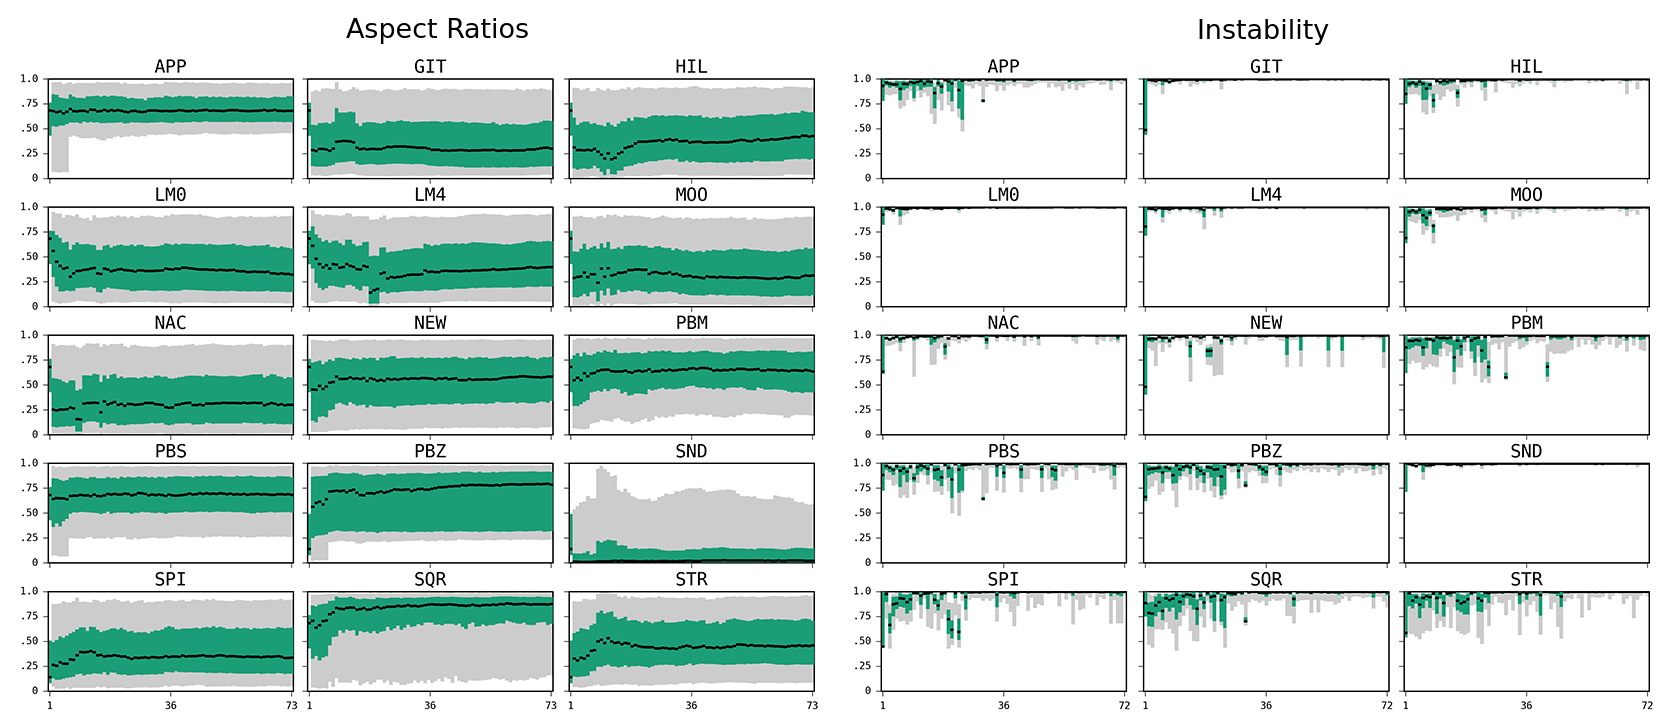
\includegraphics[width=\textwidth]{figures/treemap-algorithm/boxplots-gimp.png}
%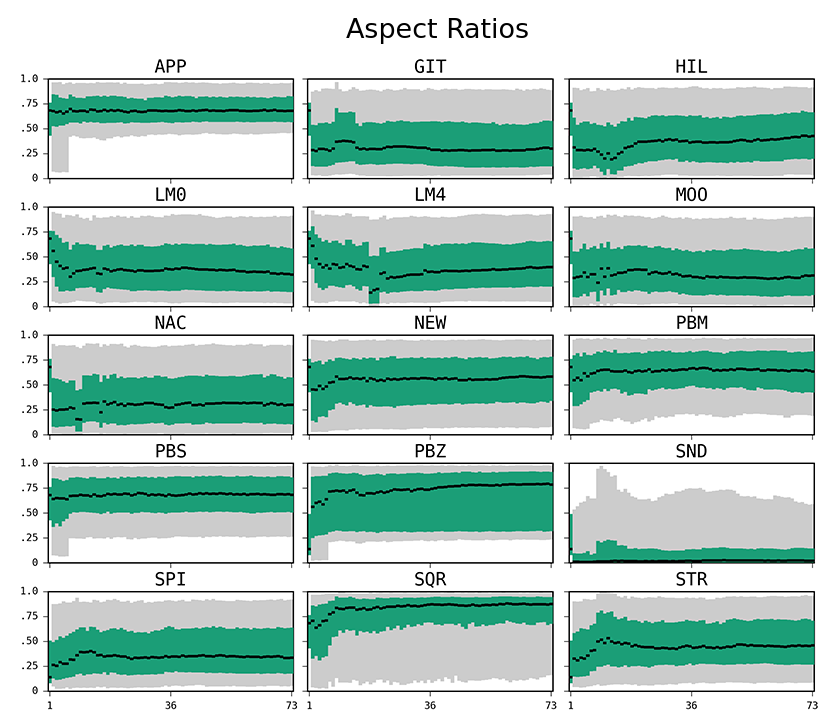
\includegraphics[width=0.69\linewidth]{figures/boxplots-gimp-ar.png}
%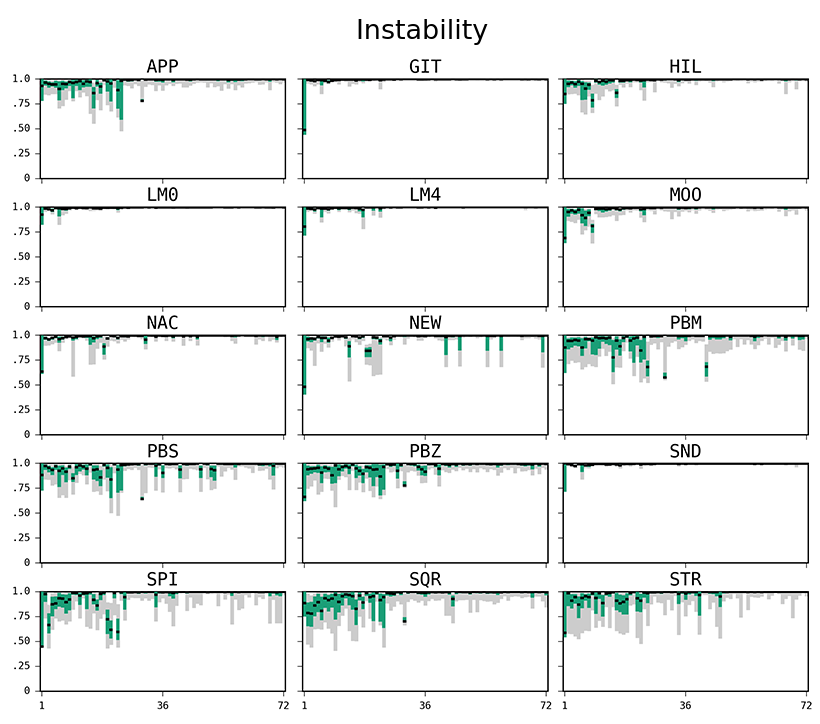
\includegraphics[width=0.69\linewidth]{figures/boxplots-gimp-st.png}
\caption{Distribution of aspect ratio ($AR, left$) and average stability ($S$, right) values over time for the GIMP dataset.}
\label{fig:boxplots}
% \end{figure*}
\end{sidewaysfigure}

While Fig.~\ref{fig:boxplots}(right) shows how the per-timestep stability changes over time, it does not show us which actual instability patterns each method is prone to deliver. Knowing this is useful, as we can better understand what to expect in terms of (undesired) cell moves from a certain algorithm, including GIT. To show this, we plot the trails connecting all centers $k_i(t)$ of all rectangles $r_i(t)$ for consecutive $t$ values over a given tree sequence (Fig.~\ref{fig:centroids}). We set the opacity of each line segment $(r_i(t), r_i(t+1))$ to the Euclidean distance $\| k_i(t) - k_i(t+1)\|$ normalized by the square root of the number of time steps. Hence, dark long lines show big moves (instability) while small moves (close to stability) are hardly visible. The image confirms the high stability of GIT --  in contrast to most other methods, except SND, GIT creates smaller cell moves (shorter dark lines), and most of these are close to horizontal or vertical. Interestingly, we see that other methods create quite different move patterns: SQR, PBS, PBZ, and PBM have mostly (large) diagonal moves. SPI shows a coil-like movement and in STR we see no vertical travel. Overall, we see that GIT is more stable not only because it yields smaller moves, but also because it constrains these to fewer motion directions, thus causes less complex dynamics (that the user must follow) in the resulting visualization. This can be also checked by watching the actual videos showing the algorithms in action~\cite{git-benchmark}.

\begin{figure*}[htbp!]
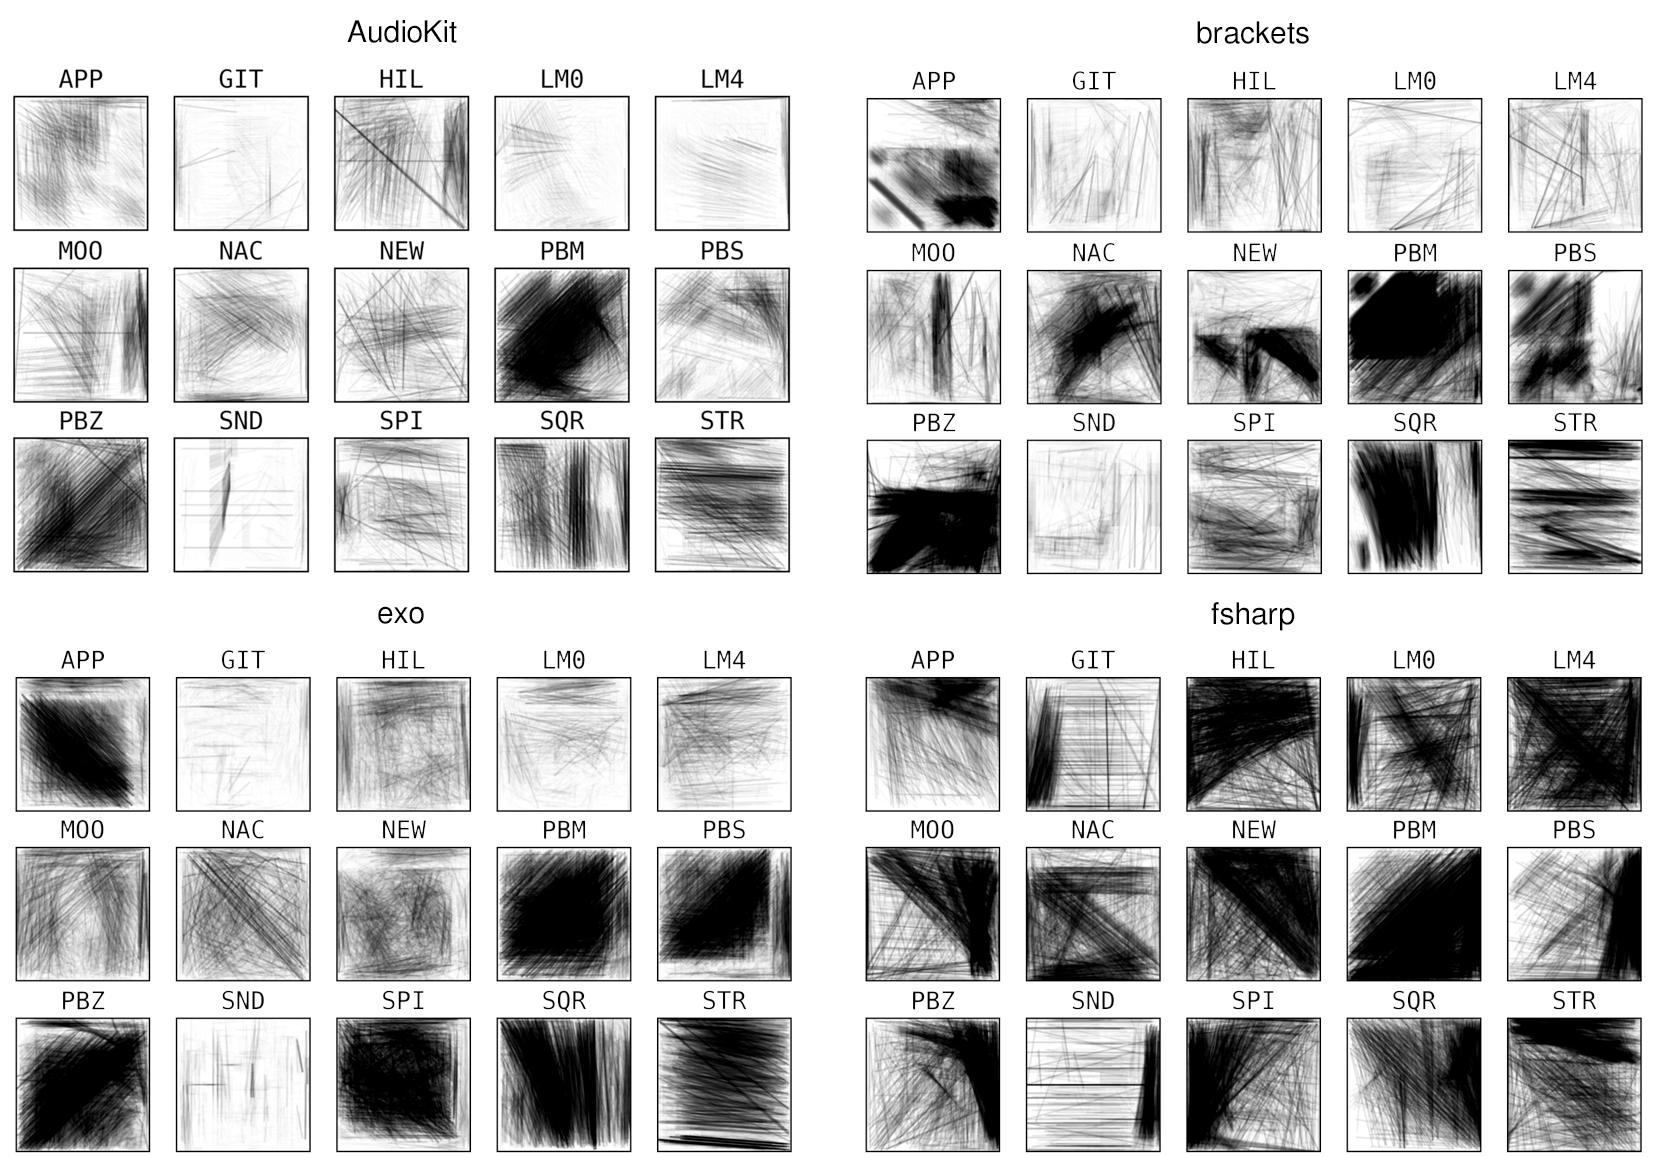
\includegraphics[width=\textwidth]{figures/treemap-algorithm/centroid-4.png}
\caption{Instability (cell center motion) patterns, all methods, \emph{AudioKit}, \emph{brackets}, \emph{exo} and \emph{fsharp} datasets.}
\label{fig:centroids}
\end{figure*}

\subsection{How do all quality metrics vary over all datasets?}
%
The experiments so far do not show the individual stability metrics (including $LD$, which can be only computed for an entire sequence), nor, for space reasons, the metrics over all 28 tested tree sequences. To get more insight in how GIT performs in these respects, we show the per-dataset average values (for $AR$ and the three stability metrics) for all tested methods, all datasets (Fig.~\ref{fig:tables}). Cells are colored using a purple (low values) to yellow (high values) colormap. We observe the following: For $AR$, APP scores consistently better for most datasets than all other tested methods. SQR reaches the highest $AR$ values, but only for a very few datasets. SND, as expected, scores overall the poorest. The remaining methods can be divided roughly into two groups, with NEW, PBM, PBS, STR, and PBZ scoring overall higher than GIT, HIL, LM0, LM4, MOO, and NAC. Concerning stability, SND scores consistently the best for all three considered metrics, and GIT, LM0, and LM4 come in the second place. This strengthens our earlier observation that GIT strikes a good balance between stability and spatial quality.

\begin{figure}[htbp!]
%\includegraphics[width=.5\textwidth]{figures/tables.png}
\includegraphics[width=.8\linewidth]{figures/treemap-algorithm/tables.png}
\caption{Average metric values for all techniques and all datasets.}
\label{fig:tables}
\end{figure}

\subsection{How to summarize GIT's quality?}
%
As noted, GIT seems to strike a good balance between spatial quality and stability. We summarize both these metrics for GIT and all other algorithms using a star plot (Fig.~\ref{fig:star-3}). The figure shows a scatterplot with $x$ mapping average stability $S$ and $y$ aspect ratio $AR$, respectively. Categorically colored points, one color per method, indicate the tested methods, attributed by their $S$ and $AR$ values over all datasets, all time steps. From each point (method), we draw lines connecting it with the $S$ and $AR$ values obtained for all the 28 tested datasets. A good algorithm has thus its `star' center placed top-right and relatively short star arms, indicating consistent quality over the entire dataset collection. We see several patterns, as follows.

At a high level, stability is roughly inversely correlated with spatial quality -- methods that score very well on one tend to score worse on the other. We see three groups of methods: APP, PBS, SQR, PBM, STR, PBZ and NEW score well on spatial quality, but poorly (except NEW) on stability. SND is the opposite outlier, scoring best on stability but clearly poorest on spatial quality. A middle group of methods (GIT, LM0, LM4, MOO, NAC, SPI, and HIL) trades well stability \emph{vs} spatial quality. Within these, GIT scores the best stability, and LM0 the best spatial quality. As such, GIT and LM0 can be considered complementary methods with respect to the stability \emph{vs} spatial quality trade-off. However, LM0 has a considerably more complex and slower implementation than GIT -- for details, we refer to~\cite{sondag17}. Separately, we see that GIT's star size (convex hull containing the lines emerging from the GIT point) is one of the smallest of all tested methods. Hence, GIT offers one of the most consistent behaviors over the entire dataset collection from all tested algorithms.

\begin{figure}[htbp!]
  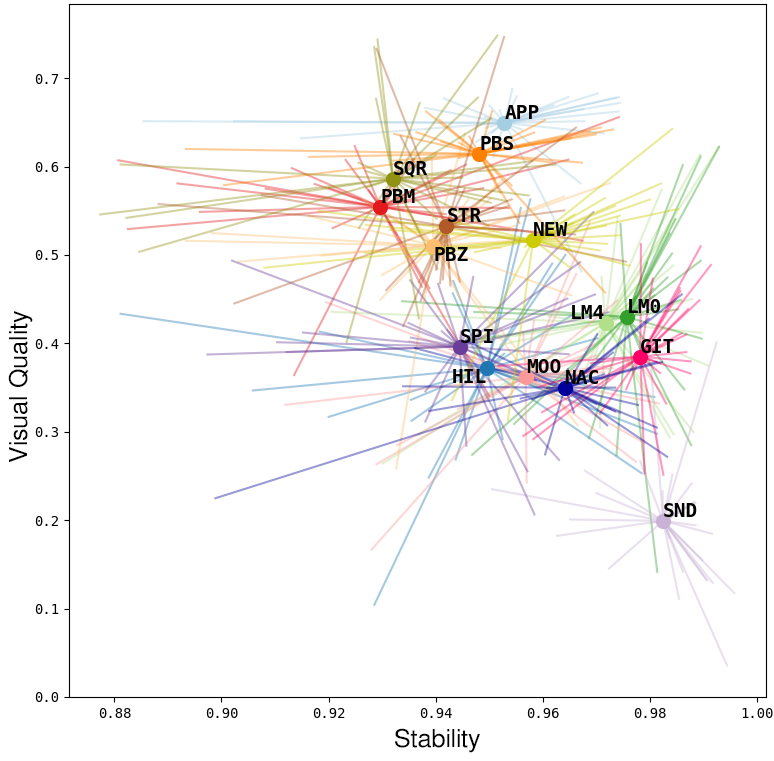
\includegraphics[width=1.0\linewidth]{figures/treemap-algorithm/star.png}
\caption{Star plot summarizing both visual quality and stability, all algorithms, all datasets.}
\label{fig:star-3}
\end{figure}

\section{Conclusion}
\label{sec:conclusion-3}
We have presented a new method for computing treemap layouts for time-dependent hierarchies. As discussed earlier, there are only a few methods in the literature that consider quality aspects pertaining to \emph{both} spatial quality and stability of such treemaps. Our contribution, in brief, is proposing a new method that takes both these quality aspects into account; and evaluating our method comprehensively on a broad dataset of 28 time-dependent hierarchies extracted from real-world dynamic dataset (software repositories), against 14 well-known treemapping methods, and using 4 quality metrics. Our results show that our new method strikes a good balance between spatial quality and stability as compared to state-of-the-art methods. Additionally, our method is simple to implement, fast, generic (with respect to the considered dynamic hierarchies), and has no hidden free parameters. More importantly, our method is an addition of a very small set of so-called \emph{stateful} methods that consider the evolution of a dynamic tree sequence when computing suitable treemaps thereof. Most existing treemapping methods are not designed to consider tree state, which arguably makes them suboptimal for handling inherently stateful datasets like dynamic trees.

Several future work directions are possible, as follows. Firstly, it is interesting to extend our evaluation to dynamic hierarchies from other domains than software evolution. This may show how much our proposal can effectively handle such more diverse datasets. Secondly, we argue that more refined quality metrics are needed (in general, for our new method but also any other treemapping methods) to capture the quality of such methods, as perceived by end users and in sync with their tasks. Finally, understanding the trade-off between the (algorithmic) reasons behind spatial quality and stability, \emph{i.e.} what to do to optimally satisfy both these requirements, is an open problem, to which we believe to have contributed to with our current work.

\chapter{Evaluating Dynamic Projections}
\blfootnote{This chapter is based on the paper ``Quantitative Evaluation of Time-Dependent Multidimensional Projection Techniques'' \citep{Vernier2020}}
\label{ch:proj-eval}
% Quantitative Evaluation of Time-Dependent Multidimensional Projection Techniques

% So far, we have explored how to use TM algos to visualize abstract, time-dependent, data. We have presented evaluations of existing TM methods, and also introduced a new concept of stability which is key to characterizing dyn treemaps. However, TMs are not the only way to visualize dynamic data. Projections are another main class of methods, useful especially when (a) the #attributes in the data is large and (b) there is no explicit data hierarchy. Similar to our work in Chs 2-3, we propose an evaluation of existing dyn proj algos. In particular, this evaluation will focus on stability, which is conceptually the same metric we introduced in Chs 2-3. We propose a stability metric for dyn projs, inspired by our earlier work on dyn TMs. Separately, we also consider visual quality (also considered in Chs 2-3 for TMs), for which we outline analogous metrics for projections. […etc]


\textit{
The first part of this thesis has explored how to use treemapping algorithms to visualize hierarchical and time-dependent data. We have presented evaluations of existing treemap methods, and also introduced a new concept of stability which is key to characterizing dynamic treemaps. We have also presented a new dynamic treemapping algorithm that scores better than existing ones on the joint requirements of stability, spatial quality, simplicity, and computational scalability. However, treemaps only address the visual exploration for weighted time-dependent hierarchical data.\\
The second part of this thesis focus on time-dependent multidimensional data, \emph{i.e.}, data with a large number or attributes or dimensions whose values change over time. 
To make sense of such multidimensional datasets, dimensionality reduction methods (or projections) represent one of the most popular and effective approaches. Similarly to the situation regarding the literature of \textbf{dynamic} treemaps, there are few works that consider \textbf{dynamic} projections, that aim to visualize time-dependent multidimensional data. 
Following the approach presented in Chapters \ref{ch:soft-eval}-\ref{ch:tree-eval}, we attack this problem by presenting here an extensive evaluation for dynamic projection algorithms, also introducing new suitable ways to define and measure the stability of such algorithms in the presence of data changes.
}

\vspace{5mm} %5mm vertical space


\noindent \textbf{Abstract:}
Dimensionality reduction methods are an essential tool for multidimensional data analysis, and many interesting processes can be studied as time-dependent multivariate datasets. There are, however, few studies and proposals that leverage on the concise power of expression of projections in the context of dynamic/temporal data.  In this chapter, we aim at providing an approach to assess projection techniques for dynamic data and understand the relationship between visual quality and stability. Our approach relies on an experimental setup that consists of existing techniques designed for time-dependent data and new variations of static methods. To support the evaluation of these techniques, we provide a collection of datasets that has a wide variety of traits that encode dynamic patterns, as well as a set of spatial and temporal stability metrics that assess the quality of the layouts.  We present an evaluation of 9 methods, 10 datasets, and 12 quality metrics, and elect the best-suited methods for projecting time-dependent multivariate data, exploring the design choices and characteristics of each method. Additional results can be found in the online benchmark repository. We designed our evaluation pipeline and benchmark specifically to be a live resource, open to all researchers who can further add their favorite datasets and techniques at any point in the future.

\section{Introduction}
%
Dimensionality reduction (DR) methods, also called projections, are used in many applications in information visualization, machine learning, and statistics. Compared to other high-dimensional data visualization techniques, projections are especially effective for datasets with many observations (also called samples or points) and attributes (also called measurements, dimensions, or variables)\,\citep{Liu2017}. Many projection techniques exist, with wide varieties of computational efficiency, ease of use, ability to preserve and/or enhance different data patterns. Surveys have also focused on assessing quantitative and qualitative aspects of projection techniques\,\citep{Nonato2019,vanderMaaten2009,Espadoto19}, thereby helping practitioners in choosing a suitable one for a given context.

Most projection techniques have been designed and evaluated only for \emph{static} data. Projecting dynamic (time-dependent) data is, however, equally important. Such data is found in most science and engineering areas, such as biology\,\citep{Teo2017}, medicine\,\citep{GRILLENZONI2019134}, and finance\,\citep{KRAPL2019101506}. The body of research in time series visualization is rich\,\citep{time0}, thereby underlining the importance of visualizing such data. Yet, there are only few examples of projecting time-dependent data\,\citep{Hu2010,Mao2007,Ward2011,bws12,Nguyen2017,Jackle2016}. Even fewer works focus on designing projection techniques specifically for dynamic data\,\citep{Rauber2016,Fujiwara2019}. In particular, it is not clear how to measure \emph{and} trade-off two key aspects of such projections: \emph{visual quality} and \emph{stability}. While visual quality was studied well for static projections, stability, seen as the ability to create a set of projections that allows users to maintain a cohesive mental map through time, is recognized as essential for dynamic data visualization\,\citep{Archambault2011,Brehmer2019ACE}, but has not been formally defined nor quantified for dynamic projections.

We work towards filling this gap in assessing projection techniques for dynamic data with the following main contributions:
\begin{itemize}
  \item We propose novel variations of existing static projection \emph{techniques} for the context of visualizing time-dependent data;
  \item We propose a set of \emph{metrics} to quantify the stability of dynamic projections;
  \item We \emph{benchmark} the visual quality and stability of dynamic projections on a dataset collection to get insights on which methods favor which of the measured quality aspects.
\end{itemize}

Our work can help researchers in targeting the identified challenges of current dynamic projection techniques, therefore potentially leading to improved ones. Separately, practitioners can use our findings into the process of determining which dynamic projection technique is best suited to their given user context. Finally, our creation of an open benchmark for assessing dynamic projections (containing datasets, techniques, metrics, visualizations, and associated workflows) should benefit both user types by providing a basis via which such techniques can be transparently compared.

The structure of this chapter is as follows. Section~\ref{sec:related} outlines related work and evaluation techniques for projections for static and dynamic data. Section~\ref{sec:experiment} details the proposed experiment we conducted to quantitatively assess the behavior of projection techniques for dynamic data, including techniques, datasets, and evaluated metrics. Section~\ref{sec:results-4} presents the obtained results. Section~\ref{sec:discussion} discusses the causes of the observed dynamic projection behavior. Finally, Section~\ref{sec:conclusion} concludes the chapter. For replication purposes, all our datasets, code, workflow, and results are openly available\,\citep{repo}.


%-------------------------------------------------------------------------
\section{Related work}
\label{sec:related}

%-------------------------------------------------------------------------
\subsection{Preliminaries}
\label{sec:preliminaries}
%
We first introduce some notation. Let
%$\mathbf{x}=(x^{1}, \ldots, x^{n}), x^{i} \in \mathbb{R}, 1 \leq i \leq n$
$\mathbf{x} \in \mathbb{R}^n$
be an $n$-dimensional sample. A revision $\mathbf{R}^t = \{\mathbf{x}_i^t\}$, or timestep, of our data consists of a set of $N$ samples $\mathbf{x}_i^t$, $1 \leq i \leq N$ measured at the same time moment $t$. A dynamic dataset $\mathbf{D}$ is a list of $T$ revisions $\mathbf{D}=\left \{ \mathbf{R}^{t} \right \}, 1 \leq t \leq T$. For simplicity of exposition and implementation, but without loss of generality, we consider next that the sample count $N$ is constant over time. In this case, $\mathbf{D}$ can be represented as a set of $T$ $N$-by-$n$ matrices, one for each timestep.

A projection technique is a function $P: \mathbb{R}^{n} \rightarrow \mathbb{R}^{q}$, where $q \ll n$. For visualization purposes, $q \in \{2,3\}$. Since 2D projections are by far the most commonly used, we next only consider the case $q=2$. We denote the projection of observation $\mathbf{x}$ by $P(\mathbf{x})$. For each timestep $t$, let $P(\mathbf{R}^{t})$ be the 2D scatterplot of all points in
$\mathbf{R}^{t}$. Finally, let $P(\mathbf{D})$ be the set of $T$ scatterplots for all timesteps of dataset $\mathbf{D}$. These can be rendered as animations, small multiples, trail sets, or other visualization encodings.

% Note that for all revisions, the number of samples $N$ remains the same, that is, there are no observations being added or removed between consecutive revisions. This is due to a limitation of the dt-SNE implementation.

Visualization of high dimensional data\,\citep{Liu2017} is a well studied topic populated with many techniques such as parallel coordinate plots\,\citep{Inselberg1990}, table lenses\,\citep{Rao2003}, scatterplot matrices\,\citep{Becker1996}, and dimensionality reduction (DR) methods\,\citep{Nonato2019,vanderMaaten2009,Espadoto19}. From all these we next focus only on DR techniques, both for static and dynamic data, and evaluation methods for both of these technique classes.

\subsection{Techniques for \textit{static} dimensionality reduction}
%
The body of research that encompasses static DR is large and spans the fields of Information Visualization and Machine Learning. There are dozens of static techniques designed to optimize different objectives and to work well under different constraints. These can be classified and categorized using several taxonomies\,\citep{vanderMaaten2009} that guide users in choosing methods that meet their requirements. We do not further elaborate on such techniques, as several surveys extensively discuss static projections. \cite{fodor02_survey} present, to our knowledge, the first survey of DR techniques covering non-linear, vector quantization, and deep learning methods. \cite{yin07_survey} surveys non-linear DR methods. \cite{bunte11} proposes a framework to quantitatively compare nine DR methods. \cite{cunningham15_survey} presents a theoretical comparison of 15 linear DR techniques. A similar survey, extended to 30 DR techniques, both linear and non-linear, is provided by \cite{sorzano14_survey}. Additional surveys look at DR methods in the larger context of high-dimensional data visualization, thus comparing and contrasting them with other visualization techniques\,\citep{buja96,hoffman02,engel12,kehrer13}. The most recent survey in this area\,\citep{Nonato2019} discusses technical aspects of DR methods, and also how such methods satisfy various user-level tasks.

\subsection{Evaluations of \emph{static} dimensionality reduction}
\label{sec:eval_static}
%
Taxonomies as the ones listed above, compare DR methods mainly from technical (algorithmic) and task-suitability aspects. An increasingly visible alternative approach is to compare techniques by measuring various quality \emph{metrics} on several techniques and datasets. A wealth of such quality metrics exist -- for recent overviews, see \citep{polzlbauer04_survey,Lee2009,lueks13,Nonato2019,Espadoto19}. Different metrics gauge different desirable aspects of a projection, and usually, several metrics are jointly used to assess DR quality\,\citep{gisbrecht15}. Just as for DR techniques, metrics can be organized using different taxonomies. Following \citep{Espadoto19}, these are as follows. \emph{Aggregate} metrics, such as trustworthiness, continuity, neighborhood hit, distance and class consistency\,\citep{sips09,tatu10}, cluster visual separation metrics\,\citep{albuquerque11,sedlmair13,sedlmair15}, and metrics that capture human perception based on machine learning\,\citep{sedlmair16} characterize an entire 2D scatterplot by a single scalar value. This is convenient when comparing (many) different scatterplots to choose a suitable one, such as in scagnostics applications. However, a scatterplot may exhibit different quality values in different areas, so a single aggregated value may not be suitable\,\citep{Joia2011,Nonato2019}. \emph{Point pair} metrics address this by measuring how point pairs $(P(\mathbf{x}), P(\mathbf{y}))$ in a projection relate to their corresponding sample pairs $(\mathbf{x}, \mathbf{y})$. These include Shepard diagrams\,\citep{Joia2011} and co-ranking matrices\,\citep{Lee2009}. Finally, \emph{local} metrics gauge separately every (small) neighborhood in a projection, thus providing the highest level of detail, and are typically visualized atop of the projection itself. These include the projection precision score\,\citep{schreck10}, stretching and compression\,\citep{aupetit07,lespinats11}, and false neighbors, missing neighbors, and average local errors\,\citep{Martins2014,Martins2015}.

Since all the above metrics aim to capture spatial aspects of the projection, we refer to them next as spatial quality metrics. Recent surveys have proposed extensive evaluations of spatial quality metrics on benchmarks containing a variety of datasets and DR methods\,\citep{Espadoto19,vanderMaaten2009}. However, time-dependent datasets were not considered.

\subsection{Techniques for \emph{dynamic} dimensionality reduction}
%
The literature is much less rich regarding DR methods that \emph{explicitly} consider dynamic data. The dynamic t-SNE (dt-SNE) method of \cite{Rauber2016} extends the well-known t-SNE method\,\citep{tsne} by adding a stability factor $\lambda$ to the objective function. Such a factor jointly minimizes the Kullback-Leibler divergence proposed by t-SNE to preserve high-dimensional point neighborhoods and also restricts the amount of motion $\| P(\mathbf{x}^{t+1}) - P(\mathbf{x}^t) \|$ that points can have between consecutive timesteps. More recently, \cite{Fujiwara2019} proposed a PCA-based method to deal with streaming data. Note that this is a harder (and different) problem from the one we aim to study since one cannot anticipate changes occurring upstream in the data when optimizing for placement of points in 2D. As such, analyzing this (and similar) methods is out of our scope. Separately, several authors use DR methods to create static maps that describe multivariate time series. \cite{Hu2010} use Self-Organizing Maps\,\citep{Kohonen1997} to create 2D trails that capture the dynamics of human motion data. \cite{Rauber2017} use similar trails, created by dt-SNE, to visualize the learning process of a neural network. \cite{Mao2007} use PCA to project text feature evolution in text sequences. \cite{Ward2011}, \cite{bws12} and, more recently, \cite{Ali2019} use similar approaches to find cyclic behavior, outliers, and trends in temporal data from medical, financial, and earth sciences domains.
%
In contrast to the previous methods, m-TSNE\,\citep{Nguyen2017} describes multivariate time series at a higher level of aggregation as single points instead of trails or polylines. Temporal MDS\,\citep{Jackle2016} projects $\mathbf{D}$ as a series of 1D projections, creating a map where the x-axis is time, and the y-axis shows the similarity of observations.

\subsection{Evaluation of \textit{dynamic} dimensionality reduction}
\label{sec:eval_dynamic}
%
Evaluating dynamic DR methods can be split into two aspects. First, just like for static DR methods, one is interested to see how well techniques capture the \emph{spatial} aspects of the underlying data. For this, one typically uses the same types of spatial quality metrics as for static projections (Sec.~\ref{sec:eval_static}). A separate important aspect for dynamic DR methods is \emph{stability}. Loosely put, stability describes how a dynamic DR technique encodes \emph{changes} in the data into \emph{changes} in the 2D metaphor used to visualize the data -- note that this definition of stability is the same as the one we used in the first part of this thesis for dynamic treemapping techniques.
Such 2D metaphors can be grouped into spatial ones, where different timesteps map to different plots, such as in small multiples; and animation-based ones, where different timesteps are encoded into frames of a 2D animation.

Stability metrics were proposed and evaluated to assess the quality of other visualizations of dynamic data such as time-dependent treemaps\,\citep{sondag17,vernier18git,vernier18software} (see also Chapters~\ref{ch:soft-eval}-\ref{ch:tree-eval}).
Stability is related to the capacity of a DR technique to deal with so-called out-of-core data. Simply put, this means the ability for a projection, created from a given dataset $\mathbf{D}$, to add extra points $\mathbf{X} \notin \mathbf{D}$ to the resulting 2D depiction $P(\mathbf{D})$, without distorting this depiction too much so that its understanding becomes hard. While recent works consider out-of-core and stability as key properties for DR projections\,\citep{Nonato2019,Boytsov2017,MateusEspadoto,Garcia-fernandez2013,Buja2008}, we are not aware of specific quality metrics that quantify these.


%-------------------------------------------------------------------------
\section{Experimental setup}
\label{sec:experiment}
%
To evaluate how dynamic DR techniques perform, we follow a methodology similar to the one proposed in \cite{Espadoto19} for evaluating static DR techniques, as follows.
We first select a set of dynamic DR \emph{techniques} to evaluate. Next, we select a collection of \emph{datasets} that cover various aspects, or \emph{traits}, that characterize high-dimensional dynamic data. Thirdly, we evaluate both spatial quality and stability \emph{metrics} on all combinations of techniques and datasets; in this step, we also propose novel metrics to gauge stability. We describe all these steps next. The analysis of the discovered correlations between techniques, dataset traits, and quality metrics obtained from our experiments is discussed afterwards in Sec.~\ref{sec:results-4}.

\subsection{Techniques}
\label{subsec:techniques}
%
We selected the dynamic DR techniques to evaluate based on the following considerations. First, we only consider techniques $P$, which, given a dataset consisting of several timeframes $\mathbf{R}^t$, produce corresponding 2D scatterplots $P(\mathbf{R}^t)$. We argue that this is the most generic definition of a dynamic projection -- from such scatterplots, other types of visualizations can be constructed next as desired (animation, small multiples, trails). This is analogous to expecting a generic static projection technique to deliver a 2D scatterplot. Hence, techniques that deliver different output types, such as m-TSNE\,\citep{Nguyen2017} and temporal MDS\,\citep{Jackle2016}, are excluded from our evaluation. Secondly, we only consider techniques that (1) are generic with respect to the input data (size, dimensionality, provenance) they can handle; (2) well-known and often used in practice, so their evaluation arguably serves a sizeable user group; and (3) easy to set up, control, and have publicly available implementations, for reproducibility. We next describe the selected techniques.\\
%replication purposes.



\noindent\textbf{t-SNE and variants:} Probably the simplest way to project dynamic data is to compute a single, global, projection $P(\mathbf{D})$ for the entire dataset $\mathbf{D}$ and next visualize the timeframes by using the desired method, be it animation, trails, or small multiples. We next call this the \emph{global} (G) approach. While this arguably favors stability (since $P$ sees all data $\mathbf{D}$ at once), it likely yields limited spatial quality, since $P$ has the challenging task of placing well \emph{all} points from \emph{all} revisions in $\mathbf{D}$. An equally simple approach is to compute independent projections $P(\mathbf{R}^t)$ for each revision $\textbf{R}^t$. We call this next the \emph{per-timeframe} (TF) approach. This arguably favors spatial quality, since $P$ must only optimize positions for each revision $\mathbf{R}^t$ separately, rather than the entire $\mathbf{D}$. However, this approach can yield poor stability, since timeframes are projected without knowledge of each other. Both the global and timeframe approaches were suggested, but not quantitatively evaluated, in the dt-SNE paper\,\citep{Rauber2016}. Given this, and also the fact that t-SNE is a very well-known static technique, we next consider G-t-SNE, TF-t-SNE, and dt-SNE in our evaluation.\\

\noindent\textbf{UMAP}: This recent DR technique\,\citep{umap} has a mathematical foundation on Riemannian geometry and algebraic topology. According to recent studies\,\citep{Espadoto19,Becht2019}, UMAP offers high-quality projections with lower computational cost and better global structure preservation than t-SNE, being thus an interesting competitor in the DR arena.  We consider in our evaluation both the global (G-UMAP) and per-timeframe (TF-UMAP) variants of this technique.\\


\noindent\textbf{PCA:} Following \citep{Fujiwara2019,Mao2007,Ward2011}, we also consider Principal Component Analysis\,\citep{pca}, implementing the global and timeframe strategies. In detail, PCA performs a linear mapping of the data $\mathbf{D}$ to, in our case, 2D by maximizing the data variance in the 2D representation. The global strategy implies computing PCA once for the entire $\mathbf{D}$. In contrast, timeframe PCA means computing PCA separately for each revision $\mathbf{R}^t$. Given the widespread use of PCA in many fields of science, and also its out-of-core ability (which, as outlined in Sec.~\ref{sec:eval_dynamic}, is related to stability), we consider both G-PCA and TF-PCA next in our evaluation.\\

\noindent\textbf{Autoencoders:} Often used in dimensionality reduction and representation learning, autoencoders\,\citep{aes,Ballard1987} are hourglass-shaped neural networks. They are composed of an encoder that takes the original data $\mathbf{D}$ and compresses it into a compact (latent) representation $P(\mathbf{D})$ of lower dimensionality (two in our case), and a decoder, which takes $P(\mathbf{D})$ and aims to reconstruct a good approximation of the original data $\mathbf{D}$. While autoencoders have been often used to create static projections of high-dimensional data, they have not, to our knowledge, been quantitatively evaluated for their ability to handle dynamic data. We evaluated four types of autoencoders, as follows. \emph{Dense autoencoders} (AE) are comprised of only fully-connected (dense) layers and are the standard variant. \emph{Convolutional autoencoders} (CAE)\,\citep{Masci2011} have both fully-connected and convolutional layers. The convolutional layers apply a non-linear transformation to the data that takes into account the spatial correlation between attributes, for instance, the proximity of pixels in an image. \emph{Variational autoencoders} may have both fully-connected layers (VAE)\,\citep{Kingma2013} and convolutional layers (CVAE). The main difference between dense and variational autoencoders is the addition of stochastic behavior in the intermediate layer of the latter. The encoder produces two vectors -- an intermediate representation (IR) and an uncertainty degree $\sigma$ for each IR value. The decoder tries to reconstruct the input through a sample from the latent space distribution with mean IR and variance $\sigma$, thus forcing the network to learn similar representation for similar inputs.
Convolutional based architectures are not generic regarding input and a meaningful spatial relationship between attributes is expected (such as found on image data). We, therefore, restrain the analysis on this document to AE and VAE. The results of CAE and CVAE runs for the image based datasets (fashion and quickdraw) can be found on the online material\,\citep{repo}.\\


\noindent\textbf{Implementation:} We implemented the chosen dynamic DR techniques (G-t-SNE, TF-t-SNE, dt-SNE, G-UMAP, TF-UMAP, G-PCA, TF-PCA, AE, CAE, VAE, CVAE) as follows. For t-SNE and PCA, we used scikit-learn\,\citep{scikit-learn} with default parameters. For dt-SNE and UMAP, we used the implementation provided online by the authors\,\citep{Rauber2016,umap}. Finally, we implemented the four autoencoder models using Keras\,\citep{chollet2015keras}, with different numbers of layers, nodes per layer, optimizers, and training routines. Tab.~\ref{tab:hyperparams} shows the values, for each autoencoder and dataset, that delivered the best results, and which we used next. The code, notebooks, and instructions to recreate our results are available online\,\citep{repo}.

\begin{table}[tb]
\centering
\fontfamily{lmss}\selectfont
\scriptsize
%\setlength\tabcolsep{2pt} % default value: 6pt
%\scriptsize
%\centering
\caption{Hyperparameters of the autoencoder-based DR methods}
% (Sec.~\ref{subsec:techniques}).}
\label{tab:hyperparams}
\begin{tabular}{llcll}
\hline
dataset    & technique & \# hidden layers & \begin{tabular}[c]{@{}l@{}}\# nodes/layer\end{tabular} & \# epochs \\ \hline
%\hline
%dataset    & technique & \begin{tabular}[c]{@{}l@{}}\# hidden layers\end{tabular} & \begin{tabular}[c]{@{}l@{}}\# nodes/layer\end{tabular} & \# epochs \\ \hline
cartolastd & AE  & 2                & 10, 10                      & 50        \\
cartolastd & VAE  & 2                & 10, 10                      & 100       \\
cifar10cnn & AE  & 2                & 10, 10                      & 20        \\
cifar10cnn & VAE  & 2                & 100, 10                     & 20        \\
esc50      & AE  & 2                & 10, 10                      & 40        \\
esc50      & VAE  & 2                & 100, 10                     & 20        \\
fashion    & AE  & 3                & 500, 500, 2000              & 40        \\
%fashion    & CAE & 4                & 32c, 32c, 32c, 1586         & 40        \\
fashion    & VAE  & 3                & 2048, 1024, 512             & 20        \\
%fashion    & CVAE & 4                & 32c, 64c, 128c, 6272        & 40        \\
gaussians  & AE  & 2                & 10, 10                      & 20        \\
gaussians  & VAE  & 2                & 100, 10                     & 20        \\
nnset      & AE  & 2                & 10, 10                      & 20        \\
nnset      & VAE  & 2                & 100, 10                     & 20        \\
qtables    & AE  & 2                & 10, 10                      & 20        \\
qtables    & VAE  & 2                & 100, 10                     & 20        \\
quickdraw  & AE  & 3                & 500, 500, 2000              & 40        \\
%quickdraw  & CAE & 4                & 32c, 32c, 32c, 1586         & 40        \\
quickdraw  & VAE  & 3                & 2048, 1024, 512             & 20        \\
%quickdraw  & CVAE & 4                & 32c, 64c, 128c, 6272        & 40        \\
sorts      & AE  & 2                & 10, 10                      & 20        \\
sorts      & VAE  & 2                & 100, 10                     & 20        \\
walk       & AE  & 2                & 10, 10                      & 20        \\
walk       & VAE  & 2                & 100, 10                     & 20        \\ \hline
\end{tabular}
\vspace{-0.15cm}
\end{table}


\subsection{Datasets}
\label{subsec:datasets}
%
There is, to our knowledge, no standardized benchmark for evaluating DR techniques. \cite{Espadoto19} took a first step towards providing such a benchmark containing 19 datasets. However, all these are time-independent, thus not suitable for us. We followed here a similar approach, \emph{i.e.} collecting a set of 10 high-dimensional and dynamic datasets that exhibit significant variations in terms of provenance, number of samples $N$, number of timesteps $T$, dimensionality $n$, intrinsic dimensionality $\rho_n$ (percentage of $n$ dimensions that explain 95\% of the data variance), and sparsity ratio $\sigma_n$ (percentage of zeros in the data). All datasets are labeled into 3 to 10 classes. We only use labels for visualization and quality assessment and not the projection itself. Table \ref{tab:datasets-4} shows the characteristics, or traits, for these datasets. Further details on them are listed below.

\begin{itemize}
  \item \textbf{cartolastd:} Player statistics for the second turn of the 2017 Brazilian football championship. Data was extracted from an open-source project\,\citep{dataset:cartola} that scrapes the Cartola FC football platform. Each timestep corresponds to a tournament round. Variables relate to per-match performance of a given player (number of goals, assistances, fouls, defenses, etc.). Players are labeled by their playing position (goalkeeper, right or left-back, defender, midfielder, forward).
  \item \textbf{cifar10cnn:} Last hidden layer activations after each training epoch for a convolutional network trained to classify the CIFAR10\,\citep{dataset:cifar10} dataset.
  \item \textbf{esc50:} Sound samples of 8 classes (brushing teeth, chainsaw, crying baby, engine, laughing, rain, siren, wind) compressed to 128 frequencies and smoothed over time. Extracted from Piczak's ESC50 dataset\,\citep{dataset:esc50}.
  \item \textbf{fashion:} 100 images from each of the 10 classes (T-shirt/top, trouser, pullover, dress, coat, sandal, shirt, sneaker, bag, ankle boot) of the FashionMNIST\,\citep{dataset:Xiao2017} dataset with decreasing amounts of noise over time.
  \item \textbf{gaussians:} Synthetic dataset used to evaluate dt-SNE\,\citep{Rauber2016}. Isotropic gaussian blobs in $nD$ with diminishing spread over time.
  \item \textbf{nnset:} Internal states (weights and biases) of several neural networks during training with the MNIST dataset\,\citep{dataset:mnist}. The networks have the same architecture but use different optimizers, batch sizes, and training-set sizes.
  \item \textbf{qtables:} Internal state of agents learning to move a car up a hill using the reinforcement learning algorithm Q-learning. The classes represent variations of learning rates and discounts.
  \item \textbf{quickdraw:} Drawing sequences for 600 objects of 6 different classes drawn by random people. Extracted from the ``Quick, Draw!'' Google AI experiment\,\citep{dataset:quickdraw}.
  \item \textbf{sorts:} This dataset was designed to compare the behavior of eight sorting algorithms. The algorithms sort different arrays of 100 random values in $[0,1]$. As they do so, we take snapshots of the intermediate states, until sorting is over. Each observed point is an (algorithm, array) run, and its feature vector is the partially sorted array at a given time.
  \item \textbf{walk:} Synthetic dataset with similar structure to \emph{gaussians}. It contains 3 high-dimensional clusters oscillate (approach, intermingle and cross, and then drift apart) in $\mathbf{R}^{100}$ over time. We designed this dataset to see how well the studied DR techniques can capture the approaching, mingling, and drifting-away dynamics mentioned above.
  % Consider 3 points in $a$, $b$, and $c$ in 1D. Each located roughly at coordinates -1, 0, and +1, respectively. Consider that point $a$ is moving in a jittery motion towards point $c$'s initial position and vice versa. Point $b$ jitters roughly around its starting position. Next, extrapolate this dynamic for 100 dimensions and 100 points for each of the three initial positions (classes).
\end{itemize}


% \red{ALEX: Very important: If these datasets come from somewhere and/or were used in other papers, SAY THIS (so we don't have to explain all about them, readers can look there). Also, within space limits, try to explain what are the attributes (or give some examples at least, if these are too many) and classes. You did this for some of the datasets but not all, so this affects next e.g. the fine-grained discussion later on, since we don't know at what kind of data we look.}

Covering all variations of high-dimensional datasets with a benchmark is already daunting for static data\,\citep{Espadoto19}, thus even more for dynamic data, as there are many types of dynamic patterns possible. Hence, we cannot claim that our benchmark is \emph{exhaustive} in terms of the space it samples. However, we believe that the included datasets exhibit a rich variety of different traits (Tab.~\ref{tab:datasets-4}). Also, no two datasets are redundant, \emph{i.e.}, have all traits similar. Given that, to date, no other benchmark exists for this task, we believe ours is a good start in supporting the intended evaluation.

\begin{table}
\centering
\caption{Datasets and their traits used in the evaluation.}
\label{tab:datasets-4}
\vspace{-0.15cm}
\includegraphics[width=.99\linewidth]{figures/projection-evaluation/datasets.eps}
\vspace{-0.15cm}
\end{table}

\vspace{-0.15cm}
\subsection{Metrics}
\label{subsec:metrics}
%
We measure the quality of all projection techniques (Sec.~\ref{subsec:techniques}) on all datasets (Sec.~\ref{subsec:datasets}) using both spatial quality and stability metrics, similarly to other evaluations of multivariate dynamic data visualizations such as treemaps\,\citep{sondag17,vernier18git,vernier18software}. In our evaluation, we use the same metrics as the survey\,\citep{Espadoto19} (and a few extra ones) over all revisions $\mathbf{R}^t$, as follows.


\subsubsection{Spatial metrics}
\label{sec:spatial-4}
%
\noindent
\textbf{Neighborhood preservation ($S_{NP}$):} With values in $[0,1]$, with 1 being the best, this is the percentage of the k-nearest neighbors of $\mathbf{x} \in \mathbf{D}$ that project in the k-nearest neighborhood of $P(\mathbf{x})$.\\

\noindent
\textbf{Neighborhood hit ($S_{NH}$):} With values in $[0,1]$, with 1 being the best, this is the fraction of the k-nearest neighbors of a projected point $P(\mathbf{x})$ that have the same class label as $P(\mathbf{x})$. Since we know that our datasets exhibit reasonably well-separated classes in $\mathbb{R}^n$, a proper DR technique (from the perspective of class separation tasks) should yield a high neighborhood hit.\\

\noindent
\textbf{Trustworthiness ($S_{Trust}$):} With values in $[0,1]$, with 1 being the best, this measures how well the $k$ nearest neighbors $NN^k(P(\mathbf{x}))$ of a projected point $P(\mathbf{x})$ match the $k$ nearest neighbors $NN^k(\mathbf{x})$ of a data point $\mathbf{x}$. Simply put, trustworthiness measures how few missing neighbors\,\citep{Martins2014} a projected point has. Formally, if $U^k(\mathbf{x})$ is the set of points that project in $NN^k(P(\mathbf{x}))$ but are not in $NN^k(\mathbf{x})$,
and $r(\mathbf{x},\mathbf{y})$ is the rank of $\mathbf{y}$ in the ordered set of nearest neighbors $NN^k(P(\mathbf{x}))$, trustworthiness is then defined as \linebreak
$1-\frac{2}{N k(2 N-3 k-1)} \sum_{x=1}^{N} \sum_{y \in U^k(\mathbf{x})}(r(x, y)-k)$.\\
%$1 - \sum_{\mathbf{y} \in U^k(\mathbf{x})}(r(\mathbf{x}, \mathbf{y})-k)$.

\noindent
\textbf{Continuity ($S_{Cont}$):} With values in $[0,1]$, with 1 being the best, this measures how many missing neighbors\,\citep{Martins2014} a projected point has. Following the above notations, let $V^k(\mathbf{x})$
be the points that are in $NN^k(\mathbf{x})$ but do not project in $NN^k(P(\mathbf{x}))$. Let also $\hat{r}(\mathbf{x}, \mathbf{y})$ be the rank of $\mathbf{y}$ in the ordered set of neighbors $NN^k(\mathbf{x})$. Continuity is then defined as \linebreak
$1-\frac{2}{N k(2 N-3 k-1)} \sum_{x=1}^{N} \sum_{y \in V^k(\mathbf{x})}(\hat{r}(x, y)-k)$.
%$1- \sum_{\mathbf{y} \in V^k(\mathbf{x})}(\hat{r}(\mathbf{x}, \mathbf{y})-k)$.

% We compute all the above metrics locally for each projection point $P(\mathbf{x})$ and, for presentation purposes, average them next as required by the analysis at hand.
In contrast to \cite{Espadoto19}, we compute neighborhood preservation, trustworthiness, and continuity for multiple (20) neighborhood sizes equally spread between $k=1\%$ and $k=20\%$ of the point count $N$. Similarly, for the neighborhood hit, we use 20 values for $k$, ranging from 0.25\% to 5\%. This allows us next to study the spatial quality of projections at different scales\,\citep{Martins2015}.\\

\noindent
\textbf{Normalized stress ($S_{Stress}$):} With values in $\mathbb{R}^{+}$, lower meaning better distance preservation, stress measures the pairwise difference of distances of points in $nD$ and $qD$. We define $S_{Stress}$ as  $\sum_{i j}\left(d_{i j}^t - \overline{d_{i j}^t}\right)^{2} / \sum_{i j} (d_{i j}^t)^{2}$,
where $d_{i j}^t$ and $\overline{d_{i j}^t}$ are the Euclidean distances between data points $\mathbf{x}_i^t$ and $\mathbf{x}_j^t$, and between their projections $P(\mathbf{x}_i^t)$ and $P(\mathbf{x}_j^t)$, respectively, for $1 \leq t \leq T$, for every point pair $(i,j)$. To ease analysis, we scale distances using standardization.\\
% $\mathbf{x}^{norm} = \frac{\mathbf{x} - X_{min}}{X_{max}-X_{min}} $
% $\mathbf{x}^{std} = \frac{\mathbf{x} - \mu(X)}{\sigma(X)}$.

\noindent
\textbf{Shepard diagram metrics:} The Shepard diagram is a scatterplot of $d_{ij}$ by $\overline{d_{ij}}$, for every pair $(i,j)$ in $\mathbf{D}$ (see Fig. \ref{fig:trails_cartolastd}b). It visually tells how different ranges of distances between points are affected by a projection. Plots close to a diagonal indicates good distance preservation.
Deviations from this highlight patterns such as poor preservation of long/short distances, creation of false neighborhoods, or stretching and compression of the manifold on which the data is defined\,\citep{Joia2011}. We summarize and quantify Shepard diagrams by measuring the relationship between the two distances. Following \cite{Espadoto19}, we use Pearson correlation to measure the linearity of the relationship, and we add Spearman and Kendall correlation to measure the monotonicity of the relationship. The three resulting correlation metrics $S_{Pearson}, S_{Spearman}, S_{Kendall}$ range from -1 to 1, where 1 means perfect positive correlation.

\subsubsection{Temporal stability metrics}
%
As previously stated, there are no metrics in the literature specially designed to measure the temporal stability of DR methods. We next propose two such metrics, as follows. The two variables whose relationship we want to measure are the \emph{change of the attributes} of a sample $\mathbf{x}$ from time $t$ to $t+1$, measured as the $n$D Euclidean distance
$ \delta^t = \|\mathbf{x}^t - \mathbf{x}^{t+1}\|$, and \emph{movement of the projection point $P(\mathbf{x})$} from time $t$ to $t+1$, measured as the 2D Euclidean distance
$ \overline{\delta^t} = \|P(\mathbf{x}^t) - P(\mathbf{x}^{t+1})\|$. Ideally, for a temporally stable $P$, we want $\overline{\delta^t}$ to be proportional to $\delta^t$. However, this may be a too hard constraint for $P$ to satisfy, just as perfect $n$D to 2D distance preservation is hard to achieve for static projections. A more relaxed requirement for a temporally stable $P$ is to have
 $\overline{\delta^t}$ a monotonic increasing function of $\delta^t$. Indeed, if this constraint were not obeyed by $P$, then if an observation $\mathbf{x}^t$ changes only slightly over time, its projection  $P(\mathbf{x}^t)$ could move a lot. That is, if  $\delta^t \ll \overline{\delta^t}$, the projection $P$ is unstable, and would convey the user the wrong impression that data is changing a lot. Conversely, if $\mathbf{x}^t$ strongly changes over time, but $P(\mathbf{x}^t)$ remains roughly static, \emph{i.e.} if $\delta_i^t \gg \overline{\delta_i^t}$, then the user gets the wrong impression that the data is not changing. Hence, for a temporally stable $P$, the two changes $\overline{\delta^t}$ and ${\delta^t}$ should be positively correlated.

To measure the relationship of ${\delta^t}$ and $\overline{\delta^t}$, we adapt the static spatial quality metrics introduced in Sec.~\ref{sec:spatial-4} as follows:\\

\noindent
\textbf{Normalized temporal stress ($T_{Stress}$):} We define temporal stress as $\sum_{i\, t}{(\delta_{i}^{t}-\overline{\delta}_{i}^{t})^{2}} / { (\delta_{i}^t)^{2}}$, where the subscript $i$ indicates sample point $\mathbf{x}_i$. As for the spatial normalized stress, we normalize distances using standardization. Low stress values indicate that the 2D changes $\overline{\delta^t}$ reflect closely their $n$D counterparts ${\delta^t}$, which is desirable.\\

\noindent
\textbf{Temporal Shepard diagram metrics:} Akin to the spatial metrics defined on Shepard diagrams, we measure the Pearson, Spearman, and Kendall correlations $T_{Pearson}, T_{Spearman}, T_{Kendall}$
between $\delta$ and $\overline{\delta}$ for every observation and consecutive timesteps. High correlation values indicate that the 2D changes $\overline{\delta^t}$ are strongly correlated with their $n$D counterparts ${\delta^t}$, which is desirable.

\alex{At this point, it is further interesting to follow the parallel of the concept of stability as defined for dynamic treemaps (Chapter~\ref{ch:tree-eval}) and as defined here above for dynamic projections, respectively. As indicated in Sec.~\ref{sec:eval_dynamic}, at a conceptual level, the two forms of stability are identical -- they both measure how much change in the visualization (treemap or 2D projection, respectively) follows the change in the data (hierarchy or $n$D dataset, respectively). However, there are some important technical differences. For dynamic hierarchies, data change in a hierarchy is hard to measure (see the discussion in Sec.~\ref{sec:stablity}), and it resides in a different space than the visual (treemap cell) change, making it hard to relate the two in a single formula. As such, for defining treemap stability, we use a proxy method based on the so-called baseline treemap. For projections, the situation is different: Both $n$D (data) and 2D (projection) spaces are of the same nature, meaning, we can quantify change in both by using Euclidean distances. Hence, we can relate both changes in a single formula (or formulas) as done above with the normalized temporal stress and temporal Shepard diagram metrics.}




%-------------------------------------------------------------------------
\section{Evaluation and Results}
\label{sec:results-4}
%
We evaluate the 12 quality metrics introduced in Sec.~\ref{subsec:metrics} on all (dataset, method) pairs formed by the selected 9 DR methods and 10 datasets, and analyze next the results. We do this by proposing several metric visualizations, from highly aggregated (to help forming first insights) to detailed (to examine more subtle points). For a direct impression, see also the videos showing the actual dynamic projections in action, available online at\,\citep{repo}.

\subsection{Aggregated results}
\label{sec:aggregate}
%

Figure~\ref{fig:aggregated} shows average metric values computed over all datasets and techniques.
% except the convolutional (variational) autoencoders (CAE, CVAE), as these techniques can only use the two image datasets (\emph{fashion} and \emph{quickdraw}), so their comparison with the other nine methods would not be fair.
Light colors represent high metric values (preferred). The colormap in Fig.~\ref{fig:aggregated} was normalized independently by the min and max of each column (metric), and it was inverted for the stress-based metrics, as low values mean preferred results for these. At the bottom of each cell, a 1D scatterplot with density mapped to luminance shows the distribution of the values of the (metric, method) pair corresponding to that cell over all datasets. The red line shows the distribution mean. The table in Fig.~\ref{fig:aggregated} is divided into three blocks: The two left blocks show spatial metrics for distance and neighborhood preservation, respectively. The right block shows stability metrics.

\begin{figure}[tb]\centering
  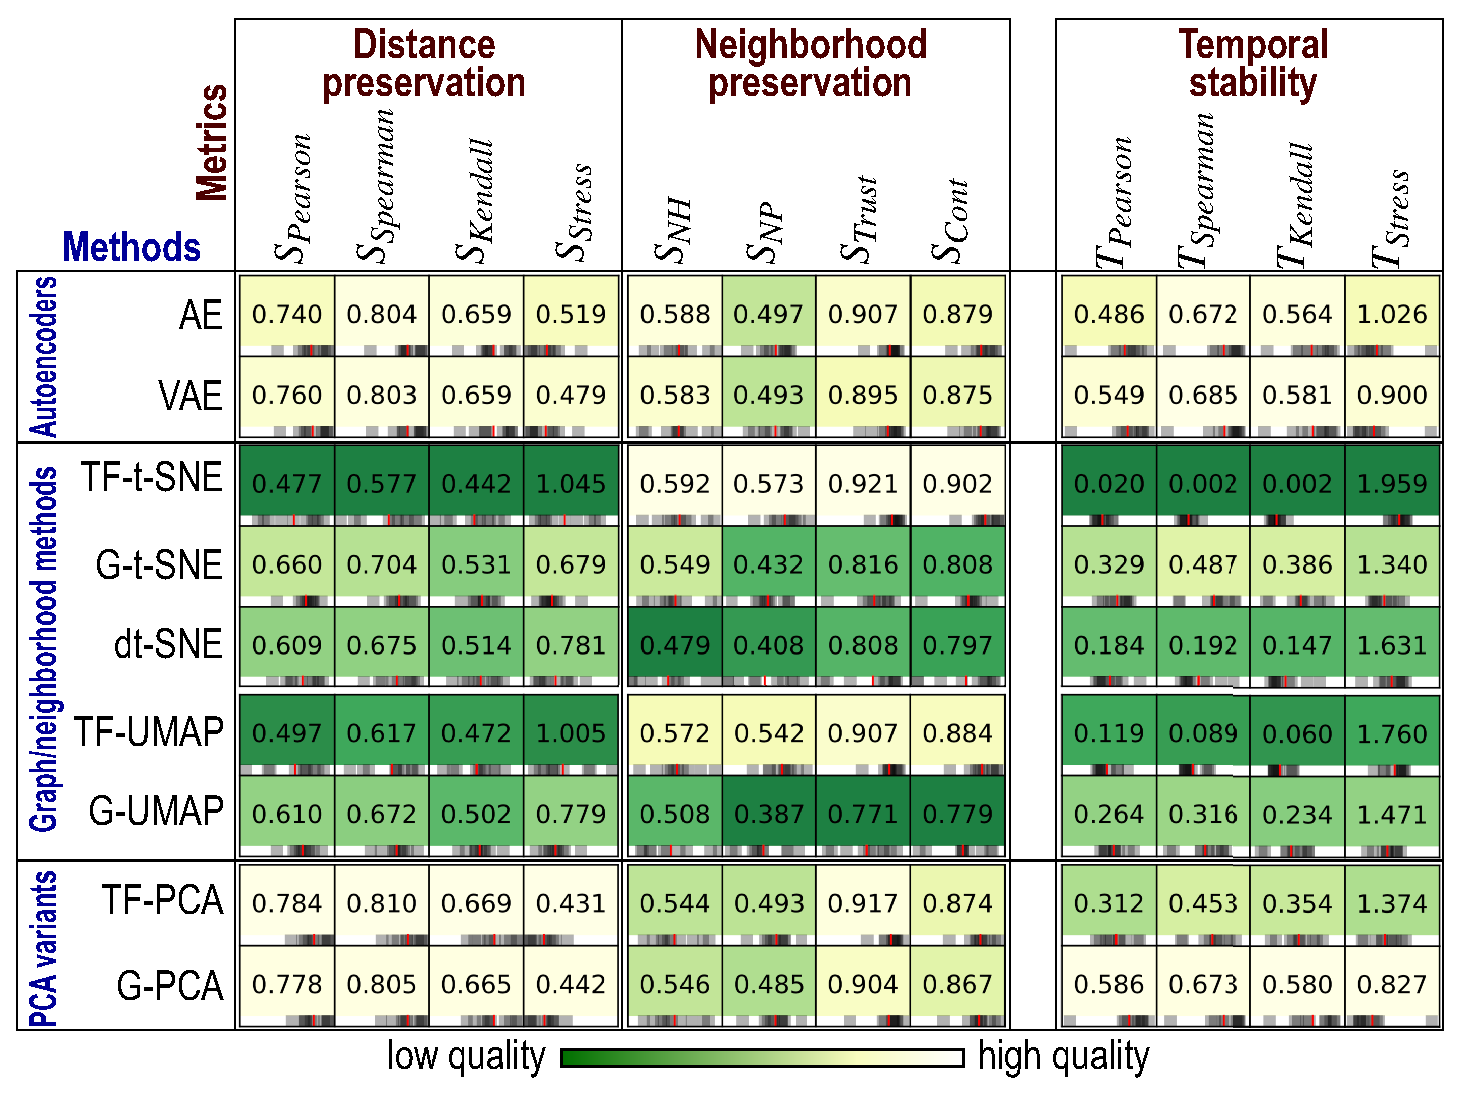
\includegraphics[width=.95\linewidth]{figures/projection-evaluation/aggregate_matrix.eps}
  \caption{Aggregated metric results over all datasets.}
  \label{fig:aggregated}
\end{figure}

\begin{figure*}[tb]\centering
  \vspace{-0.2cm}
  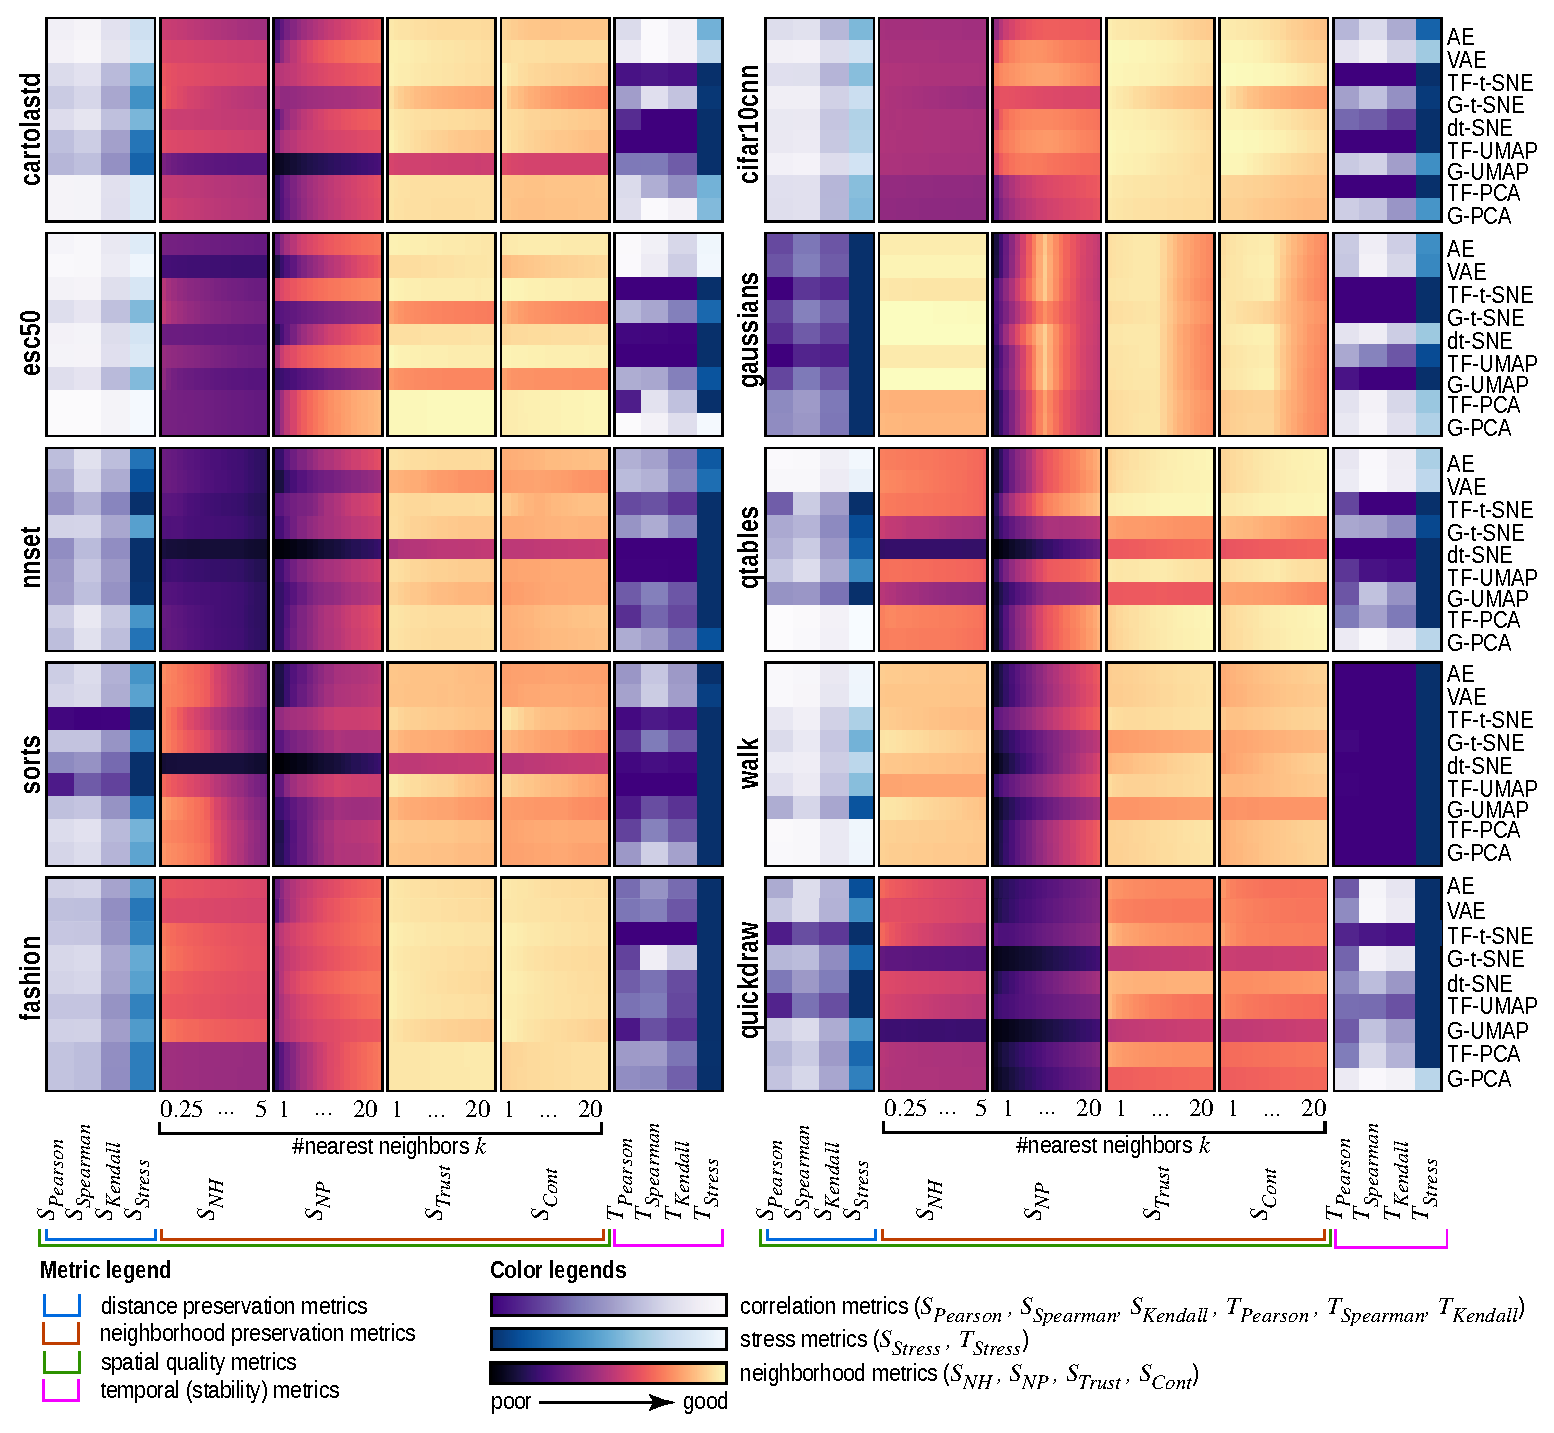
\includegraphics[width=\linewidth]{figures/projection-evaluation/f2.eps}
  \caption{Twelve spatial quality and temporal stability metrics evaluated for 9 DR  methods run on ten datasets.}
  \vspace{-0.2cm}
  \label{fig:all_datasets}
\end{figure*}


Figure~\ref{fig:aggregated} helps us to find methods that strike a balance between spatial quality and stability. In this sense, (variational) autoencoders and G-PCA score, overall, the best. The other methods are good in one aspect but not the other: Timeframe t-SNE has high neighborhood metric values but poor distance preservation and the poorest stability from all assessed methods. Timeframe PCA has high distance preservation but relatively low stability. dt-SNE appears to be as good spatially as G-t-SNE, but slightly less stable. This is an interesting finding since dt-SNE was explicitly designed (but not quantitatively assessed) to aid stability.

\subsection{Dataset-wise results}
%
Figure~\ref{fig:aggregated} is simple to read but heavily aggregated, so it does not show how the quality of specific methods depends on specific \emph{datasets}. To see this, Fig.~\ref{fig:all_datasets} shows all metric results for all datasets without aggregation. As in Fig.~\ref{fig:aggregated}, light colors mean good results. Columns are now not normalized. Column groups (a-f) represent spatial metrics, and columns (g-h) represent stability metrics. We use different quantitative colormaps to indicate different types of measured data. By examining Fig.~\ref{fig:all_datasets}, we obtain the following insights:\\

\noindent\textbf{Unstable methods:}  TF-t-SNE is always unstable regardless of the dataset. This refines the instability finding over TF-t-SNE (Sec.~\ref{sec:aggregate}) by showing that this occurs irrespective of the dataset. Also, it confirms the same observation in \cite{Rauber2016}, which, however, was not quantitatively confirmed there. The reason for this instability is the stochastic nature of t-SNE, which strongly manifests itself if we run the method from scratch on every new revision (timeframe). We could attribute the instability of TF-UMAP to the same reason.\\

\noindent\textbf{Poor spatial quality:} G-t-SNE and G-UMAP score poorly on distance and neighborhood preservation on most datasets. This is the aforementioned difficulty (Sec.~\ref{subsec:techniques}) of constructing a \emph{single} projection covering many samples in many timeframes. This is much harder than constructing a projection that preserves only neighborhoods formed by points in a \emph{single} timeframe. We see here again the trade-off between spatial quality and stability.\\

\noindent\textbf{Neighborhood preservation:}
%The four metrics $S_{NH}$, $S_{NP}$, $S_{Trust}$, and $S_{Cont}$ in Fig.~\ref{fig:all_datasets} change little as function of the neighborhood size $k$, with overall lower values for low $k$ and higher values for higher $k$. This shows that the considered projections tend to preserve larger neighborhoods better.
Here we see dataset-specific behavior: For \emph{gaussians}, $S_{NP}$, $S_{Trust}$, and $S_{Cont}$ peak at a neighborhood size of roughly 10\% of the dataset size. This makes sense since this is the size of the clusters present in this dataset -- when $k$ exceeds this value, the metrics will start considering points in other clusters, thus decrease. More interestingly, we see some outliers (dark bands in the heat-colormapped plots). These are techniques that score poorly for any $k$ value. Among these, we find G-t-SNE, dt-SNE, and G-UMAP. At the other extreme, TF-t-SNE and TF-UMAP score the best results at neighborhood preservation, followed by AE, VAE, G-PCA, and TF-PCA.\\


\noindent\textbf{Dynamic t-SNE:} In contrast to the good results qualitatively observed on the single \emph{gaussians} dataset showed in \cite{Rauber2016}, dt-SNE performs less well in both spatial quality and stability for several other of the considered datasets, being quality-wise somewhere between TF-t-SNE and G-t-SNE for all considered metrics.\\

% \begin{figure}[]\centering
%   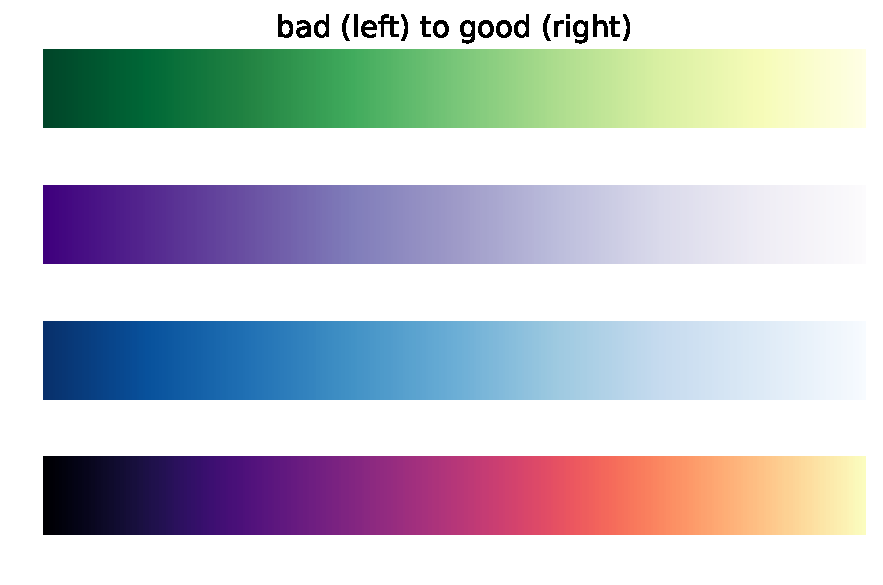
\includegraphics[width=.99\linewidth]{figures/projection-evaluation/cmaps.pdf}
%   \caption{\red{colormaps. Merge with other figures later on post processing.}}
%   \label{fig:cmaps}
% \end{figure}
%
% \begin{figure}[]\centering
%   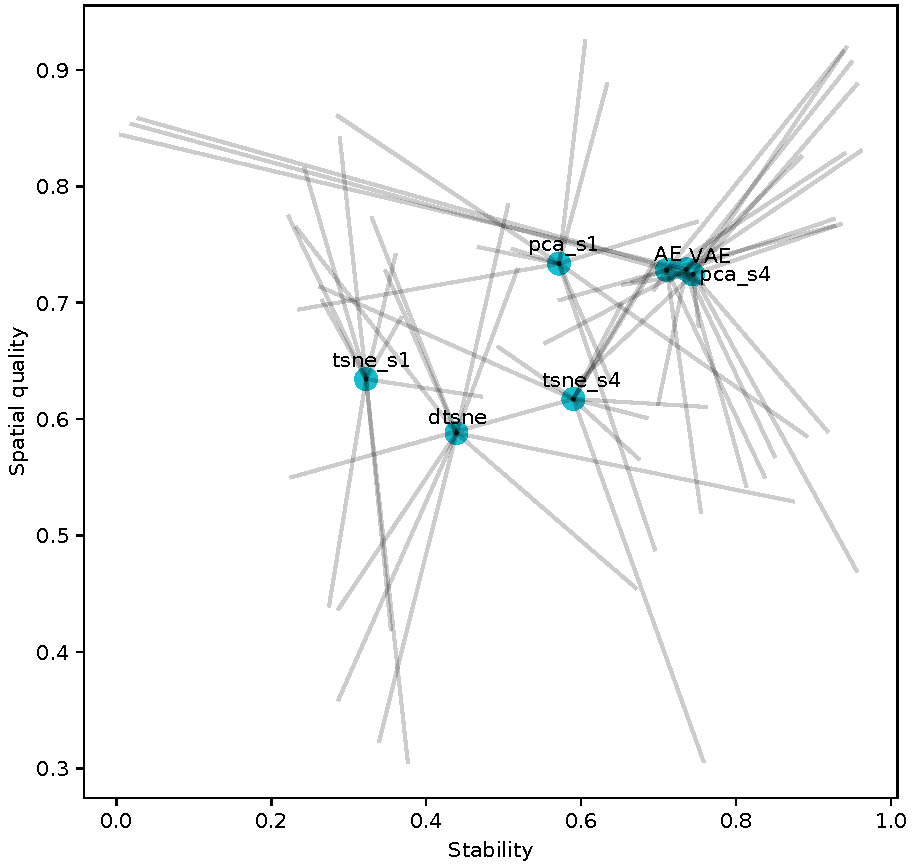
\includegraphics[width=.99\linewidth]{figures/projection-evaluation/star.pdf}
%   \caption{Star plot - \red{not sure I like this aggregation. Maybe it`s too much. ALEX: Agree; remove and replace by the two t-SNE plots of all projection techniques and all datasets.} Also see \href{https://docs.google.com/spreadsheets/d/1hfuTqH5VQadqbUBEIHHN05QlN8pKX5u8sZMd__NBAlA/edit?usp=sharing}{here}.}
%   \label{fig:star}
% \end{figure}




\noindent\textbf{Dataset difficulty:} Some datasets are considerably harder to project with good quality than others, no matter which technique we use. For example, \emph{walk} has poor stability for all techniques. In contrast, \emph{gaussians} has good stability for all techniques (except the t-SNE and UMAP variants) and good neighborhood preservation for all techniques. To study how dataset characteristics influence quality, we compute the correlation of the distance-preservation, neighborhood, and temporal stability metrics (measured over all techniques) with the six traits that we used to characterize our datasets (Tab.~\ref{tab:datasets-4}). Table~\ref{tab:corr_table} shows the results. A few things stand out: As the number of samples $N$ increases, the difficulty to preserve distances also increases, but neighborhoods are preserved better. Conversely, as sparsity $\sigma_n$ increases, it becomes harder to preserve neighborhoods. Separately, we do not find any strong (positive or negative) correlation of temporal stability with any of the traits. Overall, this suggests that the traits are useful in predicting \emph{spatial} quality of projections. However, we need additional traits that capture the data dynamics to reason about the projections' temporal stability.

\begin{table}[tb]
\centering
\caption{Correlation between metric types and dataset traits.}
\label{tab:corr_table}
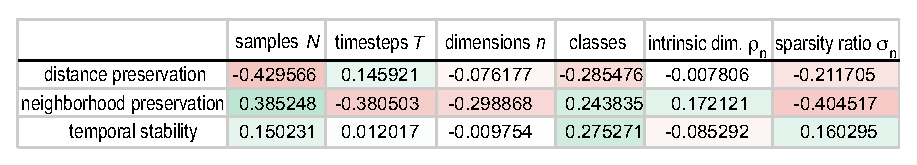
\includegraphics[width=1.01\linewidth]{figures/projection-evaluation/corr_table.eps}
\end{table}

\begin{figure*}[tb]\centering
\hspace*{-0.02\linewidth}
  \includegraphics[width=1.0\linewidth]{figures/projection-evaluation/detailed_cartolastd.pdf}
  \caption{Detailed analysis of distances and movements produced by all DR techniques on the \emph{cartolastd} dataset. \alex{Maybe rotate this fig so it becomes bigger.}}
  \vspace{-0.15cm}
  \label{fig:trails_cartolastd}
\end{figure*}

\begin{figure*}[tb]\centering
  \includegraphics[width=\linewidth]{figures/projection-evaluation/instability.eps}
  \caption{Examples of instability in TF-t-SNE (a,b) and TF-PCA (c,d,e).}
  \vspace{-0.15cm}
  \label{fig:instability}
\end{figure*}


\subsection{Fine-grained analysis}
%
While Fig.~\ref{fig:all_datasets} shows all computed metrics for each (dataset, method) combination, metric values are still aggregated to a single scalar per combination. This does not show how metrics vary over the \emph{extent} of a projection and/or over \emph{time}. There are more patterns in dynamic projections than we can capture by a set of metrics, no matter how good these are. To get such insights, we next present a fine-grained analysis that aggregates the metrics even less (see Figure~\ref{fig:trails_cartolastd}) for a single dataset (\emph{cartolastd}, chosen as it is alphabetically the first in our benchmark).
%, and all techniques, except CAE and CVAE which, as explained, are designed for spatially arranged data.
Similar visualizations for all other datasets in the benchmark are available online\,\citep{repo}. We next analyze these methods for this dataset from several perspectives, as follows.\\

\noindent\textbf{Stability visual assessment:} Figure~\ref{fig:trails_cartolastd}a shows the actual dynamic projections with point trails $(P(\mathbf{x}_i^1),\ldots, P(\mathbf{x}_i^T))$, one per player $i$. Colors map the players' labels. This visualization already says a lot about the behavior and similarities of the studied DR methods (see also the submitted videos). The instability of TF-t-SNE and TF-UMAP becomes apparent, as their trails cover a very large area in the projection space. However, these methods achieve a quite good separation of same-label clusters. In contrast, dt-SNE shows trails that depict much local movement. Both PCA variants show relatively little movement, with points oscillating along two main axes, which are the main eigenvectors computed by the methods. At the other extreme, AE, VAE, and G-t-SNE show the least motion. However, this does not imply by itself a high quality: G-t-SNE, for instance, achieves indeed a better visual spreading of samples in the available projection space, but it has very poor neighborhood preservation (see G-t-SNE results in Fig.~\ref{fig:all_datasets}) and, as already discussed above, it also has very poor stability.\\

\noindent\textbf{Distance preservation:} Figure~\ref{fig:trails_cartolastd}b shows the Shepard diagram of distances, which is a scatterplot of $d_{ij}$ by $\overline{d_{ij}}$, for every pair $(i,j)$ in $\mathbf{D}$, that helps us understand the distance preservation aspect of each technique. We see that the AE and PCA variants have overall better distance preservation (plots closer to the diagonal) than the t-SNE/UMAP variants. Also, we see that AE and PCA typically \emph{compress} $n$D distances to 2D (points mainly under the main diagonal), whereas the t-SNE/UMAP variants both compress and stretch these (points are located both under and above this diagonal).\\

Inspired by the Spearman and Kendall correlations, we consider next the agreement of \emph{ranks} instead of aggregating it to a single value. Figure~\ref{fig:trails_cartolastd}c shows this, for distance preservation, by a histogram of the \emph{absolute} rank differences of $n$D and 2D distances between point pairs. In a projection with $S_{Spearman} = S_{Kendall} = 1$, such differences would be minimized, \emph{i.e.}, the $k^{th}$ largest 2D distance $\overline{d_{ij}}$ should correspond to the $k^{th}$ largest $n$D distance $d_{ij}$ for every point pair $(i,j)$. In this case, all rank differences are zero, which would yield a histogram showing a single high bar at zero (left of the histogram). Significant rank differences spread the histogram to the right, showing poor monotonicity between the two variable ranks. From these plots, we see, again, that AE and VAE score the best, followed by G-PCA, TF-PCA, and then the t-SNE and UMAP variants.\\

\noindent\textbf{Stability metrics:} Figure~\ref{fig:trails_cartolastd}d shows Shepard diagrams for the point movements, \emph{i.e.}, scatterplots of $\delta$ by $\overline{\delta}$ for every sample compared to itself in the next timestep, for all timesteps. Note that, in these scatterplots, every point is a \emph{sample}, whereas in the classical Shepard diagrams (Fig.~\ref{fig:trails_cartolastd}b), every point is a \emph{pair} of samples. Ideally, we want $\delta$ to be positively correlated to $\overline{\delta}$, which means a plot close to the main diagonal.
The AE and PCA variants show the closest plots to the main diagonal, thus, best stability. At the other extreme, TF-t-SNE shows widely varying 2D change for similar $n$D change, thus, high instability. Finally, Figure~\ref{fig:trails_cartolastd}e shows the absolute rank difference histograms for change. Their interpretation follows the one for the distance-preservation histograms (Fig.~\ref{fig:trails_cartolastd}c):
Left peaked histograms indicate high stability, whereas flatter ones indicate a discrepancy in 2D \emph{vs} $n$D changes. These histograms strengthen the insights obtained so far, making it even clearer that the AE and G-PCA methods are far stabler than the t-SNE, UMAP and TF-PCA.


% \begin{figure*}[]\centering
%   \includegraphics[width=.75\linewidth]{figures/projection-evaluation/trails.png}
%   \caption{\red{not sure if I want to keep this due to space.}}
% \end{figure*}


\vspace{-0.15cm}
\section{Understanding dynamic projection behavior}
\label{sec:discussion}
%
The coarse-grained and fine-grained analyses presented so far highlighted that there are significant differences in the behavior of dynamic DR methods that depend on both the method and the dataset.
In this process, we also saw that visual quality and stability seem to be, in general, mutually competing for concerns -- methods that are good in one are not the best in the other.
We further explore these observations as follows. First, we analyze the causes of the observed (lack of) stability and link these to the way the studied DR techniques operate (Sec.~\ref{sec:unstable}). Next,
we summarize all our findings and propose a workflow to assist the practitioner in selecting a suitable DR technique for projecting dynamic data (Sec.~\ref{sec:choice}).

\begin{figure*}[!tb]
\centering
\includegraphics[width=\linewidth]{figures/projection-evaluation/summary_plots.eps}
\caption{Projection of projections map showing the similarity of all evaluated techniques on all datasets (Sec.~\ref{sec:choice}).}
\label{fig:tsne_0}
\vspace{-0.15cm}
\end{figure*}


\subsection{Analysis of (un)stable behavior}
\label{sec:unstable}
%
Beside empirically measuring and observing that different DR techniques have widely different stabilities, it is useful to analyze the \emph{causes} of these differences, which we do next.\\

\noindent\textbf{t-SNE and UMAP:} Our results tell that TF-t-SNE and TF-UMAP, that is, projections computed independently for each timestep, are the most unstable of the assessed techniques.
This is so since these are stochastic methods that optimize non-convex objective functions using randomly seeded gradient descent. Hence, different runs with the same data can create projections where different clusters might be formed and/or placed at different 2D positions. Figure~\ref{fig:instability}a,b shows the last scenario. From timesteps 1 to 2 of the TF-t-SNE run of the \textit{fashion} dataset, even though the local structure remains the same, the absolute position of the points and clusters changes drastically. In conclusion, using t-SNE/UMAP independently per timeframe is definitely not a good option for dynamic data.\\

\noindent\textbf{dt-SNE:} We encountered several cases where dt-SNE seems to have trouble optimizing its objective function -- for details, see the videos for \textit{qtables} and \textit{sorts}. In both these cases, dt-SNE did not capture any of the spatial structures present in the data, nor produced any sensible movement. These visual findings can be confirmed by the dark lines (low-quality values) in Fig. \ref{fig:all_datasets}. We also noticed that dt-SNE is very sensitive to the choice of hyperparameters. Concluding, whereas the initial findings in \cite{Rauber2016}, obtained on a single dataset (\emph{gaussians}) position this technique as a good option for projecting dynamic data, our additional findings raise questions about the practical value of this technique.\\

\noindent\textbf{PCA:} We also see instability in TF-PCA, but for different reasons than the ones discussed above. Specifically, if there is a change in rank of the top two eigenvectors from timestep $t$ to the next one, \emph{i.e.}, one of the associated eigenvalues becomes larger than the other, the projection exhibits an artifact that resembles a \emph{reflection} -- see the \emph{quickdraw} dataset in the two timesteps in Fig.~\ref{fig:instability}b,c. Alternatively, if the data changes sufficiently for the eigenvectors to change considerably, the projection shows a \emph{rotation}-like artifact -- see the two timesteps in Fig.~\ref{fig:instability}d,e. In contrast to t-SNE and UMAP, these artifacts are not due to stochastic seeding, but due to the way PCA works. Given the above, it is now clear why G-PCA is very stable -- it chooses the two largest-variation axes for the \emph{entire} dataset (all timesteps). The price to pay for this stability is that G-PCA may not yield the axes that best describe the data variation at each timestep, thus not the best spatial quality.\\

\noindent\textbf{Autoencoders:} Similarly to G-PCA, these techniques are stable since they train with the entire dataset (all timesteps) to learn a latent representation that encodes the global data distribution. Once trained, the encoder is a deterministic function that maps $nD$ data to 2D. The main disadvantage of autoencoders over G-PCA is usability: PCA is simple to implement and use. Autoencoders, in contrast, have the `usual' deep learning challenges, most notably finding the optimal network architecture and hyperparameter values.

% Figure \ref{fig:inverse_proj} gives us intuition about the inner workings of an AE. On the first plot, we see the output of the encoder when we input nD data ($enc :nD \rightarrow qD$), in this case, the last revision of the \textit{quickdraw} dataset. We can see class separation and a set of clusters. Conversely, the bottom image is the result of entering a uniform grid of 2D points into the decoder and getting as output the corresponding nD reconstructions ($dec :qD \rightarrow nD$). This second plot gives us a good idea of what is happening in the latent space. If we look at matching regions on the two plots, we can see that the reconstructed inputs look alike the original data in nD. That is, we see the cellos (orange dots) on the top left corner of the top plot, and matching decoded images that resemble cellos on the plot below. At the bottom left of the first plot we see the baseball cluster and matching reconstructions that resemble rounded shapes on the bottom plot. We can also see regions were classes merge and how their reconstructions combine. This static global map, which represents the shape of the latent space, provides stability to autoencoders.


% \begin{figure}[htb]
% \centering
% \includegraphics[width=.9\linewidth]{figures/projection-evaluation/inverse_proj}
% \caption{Projection of the last revision of \textit{quickdraw} and its latent space map.}
% \label{fig:inverse_proj}
% \end{figure}


\subsection{Finding similarly behaving techniques}
\label{sec:choice}
%
Figure~\ref{fig:aggregated} showed a high-level aggregated view of the quality metrics of the studied DR techniques, outlining that the autoencoders and PCA variants score better, in general, on both spatial quality and stability, than graph neighborhood techniques (t-SNE, dt-SNE, and UMAP). However, that image (and related analysis) was too aggregated. At the other extreme, Fig.~\ref{fig:all_datasets} and related discussion showed a fine-grained analysis of all metrics measured for all techniques run on all datasets. From both these analyses, it is quite hard to understand how (and when) different techniques behave similarly. This is arguably important for practitioners interested in choosing a technique in a given context (dataset type and metrics to maximize).

Figure~\ref{fig:tsne_0} supports this similarity analysis, as follows. Each point is here a technique run on a dataset, attributed by the computed 12 quality metrics. We project these points to 2D using UMAP, thus, creating a `projection of projections' map. The four images in Fig.~\ref{fig:tsne_0} use different visual codings to reveal several insights, as follows. Image (a) shows the techniques and datasets, coded by glyph, respectively categorical colors. Points in this plot are clustered more due to \emph{datasets} than \emph{techniques} -- that is, quality is more driven by the dataset nature than by which projection technique is used. For instance, we see the \emph{sorts} dataset well-separated as the purple cluster bottom-left in Fig.~\ref{fig:tsne_0}a. Images (b-d) show the same projection, colored by stability, distance preservation, and neighborhood preservation, respectively. The left part of the projection (orange dashed line, Fig.~\ref{fig:tsne_0}b) shows cases where stability and distance (and/or neighborhood) preservation are mutually complementary, \emph{i.e.}, when we obtain high stability, we get low distance/neighborhood preservation and conversely. The top-right part of the projection  (red dashed line, Fig.~\ref{fig:tsne_0}b) shows cases where both stability and spatial quality are quite high. All these cases use the AE, VAE, and G-PCA techniques. The central area of the projection is covered mainly by t-SNE, dt-SNE and UMAP, telling that these projections have average behavior (as compared to autoencoders and PCA variants). Looking at the color-coded plots (images b-d), we see that these projections do not score highest on any of the considered metrics.


% \begin{figure}[htb]
% \centering
% \includegraphics[width=\linewidth]{figures/projection-evaluation/tsne_0}
% \caption{\red{see FigureExplanation.odt for details.}}
% \label{fig:tsne_0}
% \end{figure}


The plots in Fig.~\ref{fig:tsne_0} can guide choosing a DR technique to project dynamic data: Given a dataset $\mathbf{D}$ to project, (1) find the most similar dataset $\mathbf{D}'$ in the benchmark, \emph{i.e.}, that contains data of similar nature (\emph{e.g.}, natural images, sounds) and is obtained via a similar acquisition process; (2) decide what is important for the dynamic projection of $\mathbf{D}$ -- stability, distance preservation, neighborhood preservation, or a mix of them; (3) find the projection techniques $P$ in the respective quality plots that have the desired qualities on $\mathbf{D}'$, and possibly also consider other projection techniques that behave similarly (close points in the plots). These techniques $P$ are then good candidates to project $\mathbf{D}$ with.

\section{Conclusion}
\label{sec:conclusion}
%
This chapter is an initial step towards understanding the behavior of dimensionality reduction techniques in the context of dynamic/temporal data. We hope that the information and results presented here help practitioners who want to understand their complex data and that this work can be used by authors interested in developing DR techniques as a tool for evaluation and comparison.
We proposed a publicly available benchmark with 9 methods, 10 datasets, and 12 quality metrics. To evaluate the viability of different techniques for the task, we computed spatial and temporal stability metrics for all possible combinations, thus providing an extensive collection of results. Based on the results, we presented a discussion that elaborates on the causes for understanding the dynamic behavior. All our experiments are documented and detailed online \citep{repo} to allow further analysis and reproducibility.

There are many ways this work can be extended in the future.
The benchmark can be extended with new methods, a better way to choose hyperparameters, new datasets, and new metrics. With a larger number of datasets, we can perform a robust test of the impact of dataset traits on the metrics.
We can also integrate streaming data techniques, datasets, and tests. In this sense, it is definitely interesting to consider a more principled sampling of the `universe' of all dynamic high-dimensional datasets, in the same way we considered the sampling of the universe of dynamic weighted hierarchies for the treemap evaluation in Chapter~\ref{ch:tree-eval}. This is a challenging endeavor, since we need to define relevant traits that describe different classes (types) of such datasets, as well as their dynamics. An equally challenging issue is finding representatives (samples) for these dataset classes. For treemaps, while difficult, we managed to find the relevant dynamic hierarchies, as there is a wide offer of such hierarchies from various data sources. For dynamic multidimensional datasets, we found it comparatively far harder to locate such datasets in the public domain. As such, forming a good impression of what are relevant traits for these datasets, and next collecting relevant samples to evaluate dynamic projections, is an endeavor that we leave for future work.

\alex{I adapted a bit the conclusion to make again parallels with the treemap evaluation.}

\newpage
    

\chapter{Guided Stable Dynamic Projections}
\blfootnote{This chapter is based on the paper ``Guided Stable Dynamic Projections'' \citep{Vernier2021}}
\label{ch:proj-algo}
% In Ch 5, we evaluated dyn projs from the dual perspective of visual quality and stability, just as we did for dyn TM algos in Chs 2-3. And, just as for the dyn TM algos, we found that there is no winning dyn projection that scores best for both vis quality and stability. In this chapter, similar to our earlier attempt in Ch 4 to improve dyn TMs, we aim to improve dyn projections from the perspective of the two aforementioned metrics.  For this, we propose two new dyn proj algos [….etc etc, link to the existing abstract]

\textit{
In Chapter \ref{ch:proj-eval}, we evaluated dynamic projections from the dual perspective of visual quality and stability, just as we did for dynamic treemap algorithms in Chapters \ref{ch:soft-eval}-\ref{ch:tree-eval}. And, just as for dynamic treemap algorithms, we found that there is no winning dynamic projection method that scores best for both visual quality and stability. In this chapter, similar to our earlier work in Chapter \ref{ch:git} to improve dynamic treemaps, we aim to improve dynamic projections from the perspective of the two aforementioned metrics. For this, we propose two new dynamic projection algorithms: PCD-tSNE and LD-tSNE. The former uses information given by the Principal Components of the data over all timesteps to stabilize tSNE. The latter makes use of landmarks that guide points through stable trajectories. We compare these two new algorithms with existing methods for dynamic projection, and show their advantages, following the benchmark proposed in Chapter~\ref{ch:proj-eval}.
}

\vspace{5mm} %5mm vertical space


\noindent \textbf{Abstract:}
Projections aim to convey the relationships and similarity of high-dimensional data in a low-dimensional representation.
Most such techniques are designed for static data. When used for time-dependent data, they usually fail to create a stable and suitable low dimensional representation.
We propose two dynamic projection methods (PCD-tSNE and LD-tSNE) that use global guides to steer projection points. This avoids unstable movement that does not encode data dynamics while keeping t-SNE's neighborhood preservation ability. PCD-tSNE scores a good balance between stability, neighborhood preservation, and distance preservation, while LD-tSNE allows creating stable and customizable projections. We compare our methods to 11 other techniques using the quality metrics and datasets presented in \cref{ch:proj-eval}.
    
\section{Introduction}
%

Many domains produce datasets with large numbers of observations (also called samples or points) and attributes (also called measurements, dimensions, or variables). Dimensionality reduction techniques, also called projections, are an established tool for visualizing such datasets in a simplified, compact, and scalable way.

The literature on static projections -- that address the visualization of time-independent datasets -- is quite rich, with many techniques, surveys, and benchmarks on the subject\,\citep{Nonato2019,Espadoto19,sorzano14_survey,cunningham15_survey}. In contrast, far fewer techniques and comparisons thereof exist for projecting time-dependent datasets, in which the sample values change over time -- which is a much harder problem.

Besides faithfully capturing the data structure -- a desiderate shared with static projections -- dynamic projections also face the challenge of maintaining temporal coherence. Failing this will create false motion artifacts in the projection, which can mislead the user into thinking there are data changes where none exist, or conversely. Figure~\ref{fig:demo-instability} illustrates this: We have a 100-dimensional dataset of 2000 samples covering 10 distinct isotropic Gaussian distributions that collapse in linear trajectories into 10 single points over 10 timesteps\,\citep{Rauber2016}. The images depict the results of three dynamic projection techniques (G-PCA, TF-PCA~\citep{pca}, and TF-tSNE~\citep{vanderMaaten2008}) for this dataset, showing the trajectories of all data points over the ten timesteps. Knowing the dataset, we can tell that G-PCA renders quite faithfully the data dynamics and structure; TF-PCA creates an artificial amount of spiraling; and TF-tSNE creates a very large amount of apparently random and unstable motion that is not present in the data. If such variability in the projection results is seen for this simple, synthetic dataset, the choice of a good dynamic projection method for real-world datasets is clearly very hard.


% \red{There are different ways to project a dynamic dataset \red{(cite a few non-animation works)}, but we will focus on creating animation-like representations, where we project the $N$ samples of the original dataset into $2D$ space for each timestep $t$, as demonstrated in Fig.\,\ref{fig:animation}.}

% % https://docs.google.com/drawings/d/15hzYRNaO8qreoUQrndlu_6f5Sn1c8ebI0HuE5yEEOVY/edit
% \begin{figure}[!h]\centering
%   \includegraphics[width=\linewidth]{figures/projection-algorithm/gaussians-pca-s4.png}
%   \caption{caption}
%   \label{fig:animation}
% \end{figure}

% https://docs.google.com/drawings/d/1XENnHkpmsl6AqJfx5l2b-H4bSuKonbjgjYY_E599Q5c/edit
\begin{figure*}[h]
 \centering
 \includegraphics[width=\linewidth]{figures/projection-algorithm/demo-instability-trails-rebuttal-with-color-3.eps}
%  \includegraphics[width=0.48\linewidth]{figures/projection-algorithm/demo-instability-trails-rebuttal-with-color.pdf}
 \caption{A time-dependent collapsing 100-dimensional 10-Gaussian-distributions dataset (2000 points) is visualized by three projection methods. Point trails are colored by time (top) and class (bottom). The images show increasing amounts of instability artefacts.}
 \label{fig:demo-instability}
 \vspace{-0.15cm}
\end{figure*}

Motivated by these challenges of understanding and quantifying the quality of dynamic projections, in the previous chapter we evaluated nine such techniques, and came to the conclusion that there is no perfect method, and that an inherent trade-off between stability and spatial quality (i.e., neighborhood and distance preservation) exists. The methods that scored the best on both criteria were autoencoder-based methods and Global PCA. Neighborhood-based methods, such as t-SNE and UMAP, strongly showed a lack of stability. At the same time, these are among the favorite methods for static projection, given their high capability in preserving data structure.

We aim to cover the above-identified gap by proposing ways to add stability to the neighborhood preservation ability of static projections, in particular t-SNE. We propose two approaches that use global influences to steer projected points:
Our first method, LD-tSNE, offers similar flexibility in steering dynamic projections via landmarks as known for static projections, and also reaches good quality values. Our second method, PCD-tSNE, increases neighborhood influences atop an already stable Global PCA dynamic projection, scoring better than all compared counterparts in terms of spatial quality combined with stability. The global influence of both methods can be controlled via simple user parameters to find the best balance between stability and spatial quality. We compare our methods with 11 existing dynamic projections on a benchmark of 10 high-dimensional datasets using 12 metrics for both spatial quality and stability. 

Section~\ref{sec:background} overviews related work on dynamic projections of high-dimensional data. Section~\ref{sec:methods} introduces our two new methods. Section~\ref{sec:experimental-setup} presents the experimental setup we used in comparing our new methods with existing ones. Section~\ref{sec:results} presents and discusses the evaluation results. Finally, Section~\ref{sec:conclusion-5} concludes the chapter.

  
%-------------------------------------------------------------------------
\vspace{-0.15cm}
\section{Related work}
\label{sec:background}

\subsection{Preliminaries}
%
Following the same notation of \cref{ch:proj-eval}, let $\mathbf{x} \in \mathbb{R}^n$
be an $n$-dimensional sample (also called data point or observation). A timestep $\mathbf{D}^t = \{\mathbf{x}_i^t\}$ of our data consists of a set of $N$ samples $\mathbf{x}_i^t$, $1 \leq i \leq N$, 
measured at the same time moment $t$. A dynamic dataset $\mathbf{D}$ is a list of $T$ timesteps $\mathbf{D}= ( \mathbf{D}^{t} ), 1 \leq t \leq T$. For simplicity of exposition and implementation, but without loss of generality, we consider next that the sample count $N$ is constant over time. In this case, $\mathbf{D}$ can be represented as a set of $T$ $N$-by-$n$ matrices, one per timestep $t$.

A projection technique is a function $P: \mathbb{R}^{n} \rightarrow \mathbb{R}^{q}$, where $q \ll n$. For visualization purposes, $q \in \{2,3\}$. Since 2D projections are by far the most commonly used, we next only consider the case $q=2$. We denote the projection of sample $\mathbf{x}$ by $P(\mathbf{x})$. For a timestep $t$, let $P(\mathbf{D}^{t}) = \{ P(\mathbf{x}^t) | \mathbf{x}^t \in \mathbf{D}^{t} \}$ be the 2D scatterplot of the projections of all points in
$\mathbf{D}^{t}$. Finally, let $P(\mathbf{D})$ be the set of $T$ scatterplots for all timesteps of dataset $\mathbf{D}$. These can be rendered as animations (see additional material\,\citep{repo-guided}), trail sets (as in Fig. \ref{fig:demo-instability}), small multiples\,\citep{Rauber2016}, or other visual encodings. 


\subsection{Visualization of high-dimensional data}
\label{sec:rw_vis_dynamic}
%

Visualization of static high dimensional data\,\citep{Liu2017} is a well studied topic populated with many techniques such as parallel coordinate plots\,\citep{Inselberg1990}, table lenses\,\citep{Rao2003}, scatterplot matrices\,\citep{Becker1996}, and dimensionality reduction (DR) methods or projections\,\citep{vanderMaaten2009}. Compared to other methods, projections scale visually very well, being able to accommodate datasets of millions of samples and hundreds up to thousands of dimensions in limited screen space. Several quality metrics have been proposed to gauge how faithfully projections capture the structure of high-dimensional data, \emph{e.g.}, trustworthiness and continuity\,\citep{venna06}, normalized stress and Shepard diagrams\,\citep{Joia2011}, neighborhood hit\,\citep{Paulovich2008}, class consistency\,\citep{tatu10}, and distance consistency\,\citep{sips09}. Tens of different projection algorithms exist for static data; detailed taxonomies of such methods, benchmarks, and qualitative and quantitative evaluations are available in a range of surveys\,\citep{Nonato2019,Espadoto19,fodor02_survey,cunningham15_survey,sorzano14_survey,vanderMaaten2009}.

%Comparatively few works use projections to explore temporal (time-dependent) high-dimensional data. Most importantly, few authors explicitly propose techniques and strategies for creating stable projections for temporal\,\citep{Rauber2016,Vernier2020} and for streaming data\,\citep{Neves2020}.

\subsection{Strategies for dynamic projections} 
\label{sec:taxonomy}
%
All current dynamic projection techniques that we are aware of are based on methods that were initially designed for static data. These base methods are adapted to achieve two goals: (a) obtaining good \emph{spatial quality}, measured by the various static projection metrics outlined earlier in Sec.~\ref{sec:rw_vis_dynamic}; and (b) obtaining good \emph{stability}, defined as the ratio between changes, over time, of the projection $P(\mathbf{D})$ \emph{vs} changes of the data $\mathbf{D}$\,\citep{Vernier2020}. Besides projections, similar definitions of stability have been used to quantify dynamic treemapping algorithms\,\citep{vernier_treemap,vernier18software}.  We next propose to classify these techniques as a function of how they `adapt' the underlying base (static) projection algorithm, denoted further $P_B$, to handle spatial quality and stability for dynamic data.\\

%A number of these strategies were proposed by Rauber \emph{et al.} \citep{Rauber2016} using t-SNE as testbed, but were not implemented or quantitatively tested. 
%Later, Vernier \emph{et al.} \citep{Vernier2020} explored the idea further, benchmarking the proposed methods and applying these strategies to other base algorithms. These strategies, according to our taxonomy, are:

\noindent\textbf{Per-timeframe (TF):} 
In this simplest strategy, $P_B$ is applied to each timestep $\mathbf{D}^t$ to create an independent projection $P_B(\mathbf{D}^t)$. Hence, $P(\mathbf{D}) = ( P_B(\mathbf{D}^t))_{ 1 \leq t \leq T}$. In other words, the base method $P_B$ is not allowed to ``look at the past or future'' when projecting a given timestep $t$ -- it only sees the data in $\mathbf{D}^t$. Given the popularity of PCA\,\citep{pca}, t-SNE\,\citep{vanderMaaten2008}, and UMAP\,\citep{umap}, the per-timeframe strategy is often used for these base projections, leading to variants we call next TF-PCA, TF-tSNE, and TF-UMAP, respectively. Several further variations of this strategy exist. \cite{bsk16} propose time curves which connect consecutive positions $P_B(\mathbf{x}_i^t)$ of the same point $i$ for all moments $t$, using MDS for $P_B$. Similar curves have been used by \cite{bws12} (using PCA for $P_B$). \cite{Brich2020} use time curves and argue for the pro's and con's of PCA \emph{vs} MDS for $P_B$. However, none of the studied base projections was found ideal concerning stability and spatial quality. At a more general level, the same strategy was used to connect different 2D scatterplots created by other means than projections\,\citep{hkf16}. \cite{Jackle2016} use MDS for $P_B$ to project all $n$ spatial dimensions of $\mathbf{D}$ to a single dimension and use the second dimension of the screen space to map time. 
Overall, the per-timeframe strategy favors spatial quality, which can be as high as delivered by $P_B$. However, stability can be (very) low since $P_B$ is applied independently to the timeframes. \\

\noindent\textbf{Global (G):}
At the other end of the spectrum, global methods apply $P_B$ to the entire dataset, and then separate the projected points based on their timesteps, \emph{i.e.}, $P(\mathbf{D}) = (\{\mathbf{y}^t \in P_B(\mathbf{D})\})_{1 \leq t \leq T}$, where $\mathbf{y}^t = P_B(\mathbf{x}^t)$ and $\mathbf{x}^t \in \mathbf{D}^t$. Like per-timeframe, this strategy is also simple to implement. It maximizes stability by construction. As such, many applications use this strategy, \emph{e.g.} \cite{Hu2010} that project 72-dimensional human body keypoints using LLE, or \cite{Fujiwara2018} who project entire dimensions (time series) using MDS and t-SNE for computer performance analysis. The latter method was also extended to use PCA and UMAP as $P_B$\,\citep{Fujiwara2020}.

When $\mathbf{D}$ is large, either in terms of number of samples or number of timesteps, computing a single projection $P_B(\mathbf{D})$ can be expensive. Also, the spatial quality of global techniques is typically lower than for the per-timeframe strategy since $P_B$ now has to optimize the relative placement of points in \emph{all} timeframes, even if such points never co-exist at the same time. Out-of-sample projection (OOS) methods can help with these issues. Simply put, an OOS technique $P$ is constructed to optimize the projection of a subset $\mathbf{D}_s \subset \mathbf{D}$ according to one's desired quality metrics. Next, $P$ is used to extrapolate the projection to the entire $\mathbf{D}$. Out-of-sample strategies have been proposed for many static projection methods\,\citep{oos}. Recently, \cite{MateusEspadoto} have shown how to use deep learning to construct out-of-sample approximations of any static projection technique. Hence, OOS techniques can be used to accelerate and potentially increase the quality of global projection methods. However, the challenge is in how to select the small subset $\mathbf{D}_s$ so as to represent well the entire time-dependent dataset $\mathbf{D}$. To our knowledge, no studies of this aspect exist for dynamic projections.\\

\noindent\textbf{Continuous (C):} This strategy applies to base methods that iteratively optimize neighborhood configurations, such as t-SNE and UMAP. In the following, we call these variants C-tSNE and C-UMAP, respectively. The projection $P(\mathbf{D}^{t})$ continues the gradient descent from the positions of the previous timestep $P(\mathbf{D}^{t-1})$, with the updated cost function for $t$. This reduces significantly the non-deterministic behavior created by removing consecutive initialization steps. Still, this can fail to produce stable projections as points are still allowed to move significantly during optimization. Dynamic t-SNE (D-tSNE)\,\citep{Rauber2016} aims to alleviate this by adding a penalty term to the continuous strategy using t-SNE for $P_B$. This limits, up to a certain extent, too large point movements between consecutive timesteps.
Incremental PCA\,\citep{ross08} projects points in a streaming fashion and is therefore amenable to project time-dependent data. \cite{Fujiwara2020} further increase incremental PCA's stability by using Procrustes analysis to align consecutive projections, a method also proposed independently by \cite{Joia2011}. \cite{Neves2020} propose Xtreaming, an incremental technique that handles streaming high-dimensional data by continuously adapting UPDis\,\citep{updis}, a projection with out-of-sample capability, thus, good stability. Overall, continuous strategies achieve a good balance between spatial quality and stability. However, this balance can be hard to tune in practice. 

Vernier \emph{et al.}'s evaluation\,\citep{Vernier2020} found that PCA and (Variational) Autoencoders with the global strategy -- called next G-PCA, G-VAE, and G-AE respectively -- were the best-suited methods for projecting temporal data. The global strategy, however, does not seem to work well with graph or neighborhood-based methods, such as t-SNE and UMAP -- we denote these methods next as G-tSNE and G-UMAP, respectively. 

%-------------------------------------------------------------------------
\section{Guided methods for dynamic projection}
\label{sec:methods}
%
Many guided methods exist in the static projection literature\,\citep{Nonato2019,sorzano14_survey}. Simply put, all these methods select a subset of samples $\mathbf{L} \subset \mathbf{D}$ to create $P$, by extrapolating $P(\mathbf{L})$ to $P(\mathbf{D})$. Conceptually speaking, the continuous strategy (Sec.~\ref{sec:taxonomy}) can be seen as a type of guidance, where $P(\mathbf{D}^{t+1})$ is steered by the earlier projection $P(\mathbf{D}^{t})$. Similarly, the out-of-sample global strategy (Sec.~\ref{sec:taxonomy}) can be seen as a type of guidance where $P(\mathbf{D}_s)$ steers $P(\mathbf{D})$. However, even though this works for simple datasets, when the data present complex dynamics and large changes over time, existing continuous strategies become too restrictive. We propose two new guided methods for dynamic projection that use global influences (landmarks or suggested placements) to steer and stabilize the projection while still accounting for neighborhood preservation. The two methods use t-SNE as base projection given (a) t-SNE's high popularity for the static projection case; and (b) the difficulty of using t-SNE in a dynamic context (see Sec.~\ref{sec:taxonomy}), which we want to overcome.
Importantly, while guided strategies mainly aim to address \emph{scalability} for static projections, our different aim of using guidance is to address \emph{spatial quality} and \emph{stability}. 

%-------------------------------------------------------------------------
\subsection{Landmark Dynamic t-SNE (LD-tSNE)}
\label{sec:ld-tsne}
%
One idea that has been successfully used in the static case, and can be utilized to our advantage for dynamic data, is the use of \emph{landmarks}. 
Landmarks or similar control point-based mechanisms are well known and have been used to aid different tasks on static data. Examples include performance improvement~\citep{Pekalska1999,DeSilva2003,DeSilva2004,Vladymyrov2013,Paulovich2008,Kruiger2017a}, support of out-of-sample capability~\citep{Boytsov2017,Policar2019}, and projection customization~\citep{Joia2011,updis}.
Yet, we are not aware of any work that combines landmarks or control points to stabilize \emph{dynamic} projections. We use landmarks to give the base projection $P_B$ method a sense of global structure, in an attempt to reduce the instability inherent to neighborhood-based projection techniques such as t-SNE.

Two main aspects must be considered when using landmarks as guides: how to generate the landmarks and how to use the landmarks to steer points, as follows.\\

\vspace{-0.15cm}
\noindent\textbf{Landmark generation:} Each landmark $\mathbf{l}=\left(\mathbf{l}^n, \mathbf{l}^q\right)$ consists of a high-dimensional component $\mathbf{l}^n \in \mathbb{R}^n$ and a component $\mathbf{l}^q \in \mathbb{R}^q$ in the projection space.
It is important that the set $\mathbf{L} = \{ l^n \}$ captures well the structure of the high-dimensional dataset $\mathbf{D}$, otherwise the ``steering'' may become uneven. There are different ways of achieving this goal\,\citep{DeSilva2005}. For simplicity and speed, we opted to create $\mathbf{L}$ by randomly sampling $k$ points from $\mathbf{D}$, where $k$ is a fraction of the size of $\mathbf{D}$. For most of our tests, we set $k=N$, \emph{i.e.}, the number of points in a timeframe (see \cref{ch:projection-algorithm-appendix} for the precise numbers). To generate the low-dimensional points $\mathbf{l}^q$, we simply project $\mathbf{L}$ using a user-chosen method. We experimented here with both PCA and t-SNE, and selected the landmark projection which yielded the best results (more information available in \cref{ch:projection-algorithm-appendix}).\\

\vspace{-0.15cm}
\noindent\textbf{Landmark steering:} The first step towards steering is to select a neighborhood-based projection technique to use. We chose here t-SNE due to its popularity and previous good results in extending it for dynamic data\,\citep{Rauber2016}. To describe how steering takes place, let us consider the original t-SNE cost function, given by the Kullback-Leibler (KL) divergence between the joint-probability distributions $\mathcal P$ and $\mathcal Q$ that describe point-neighborhoods in $\mathbb{R}^n$, respectively $\mathbb{R}^q$
%
\begin{equation}
C_{tsne} = D_{KL}\left(\mathcal{P}||\mathcal{Q}\right) =  \sum_{i=1}^{N} \sum_{j\neq i} p_{i j} \log \frac{p_{i j}}{q_{i j}},
\label{eqn:c_tsne}
\end{equation}
%
where $ p_{ij}=\frac{p_{i | j}+p_{j | i}}{2 N}$ models the distance of two points $\mathbf{x}_i$ and $\mathbf{x}_j$ in $\mathbb{R}^n$ and
%
$$ p_{j | i}=\frac{\exp \left(-\left\|\mathbf{x}_{i}-\mathbf{x}_{j}\right\|^{2} / \left(2 \sigma_{i}^{2}\right)\right)}  
{\sum_{k \neq i}^{N} \exp \left(-\left\|\mathbf{x}_{i}-\mathbf{x}_{k}\right\|^{2} /\left(2 \sigma_{i}^{2}\right)\right)}. $$
%
Here, $p_{j|i}$ can be seen as a relative measure of similarity based on the local neighborhood of a point $\mathbf{x}_i$. The effective number of neighbors considered for each point is given indirectly by a user-chosen perplexity value $\mu$: The value of $\sigma_i$ is computed so that, for the user-given $\mu$ and each $i$, $\mu=2^{-\sum_{j}^{N} p_{j | i} \log _{2} p_{j | i}}$.

A Student's t-distribution with one degree of freedom is used to compute the joint-probability distribution in $\mathbb{R}^q$ as
%
$$q_{i j}=\frac{\left(1+\left\|\mathbf{y}_{i}-\mathbf{y}_{j}\right\|^{2}\right)^{-1}}{\sum_{k, i \neq k}\left(1+\left\|\mathbf{y}_{i}-\mathbf{y}_{k}\right\|^{2}\right)^{-1}}.
$$
The gradient of the cost function, given by
%
\begin{equation}
 \frac{\partial C_{tsne}}{\partial \mathbf{y}_{i}}=4 \sum_{j}\left(p_{i j}-q_{i j}\right)\left(\mathbf{y}_{i}-\mathbf{y}_{j}\right)\left(1+\left\|\mathbf{y}_{i}-\mathbf{y}_{j}\right\|^{2}\right)^{-1} 
 \label{eqn:grad_tsne}
\end{equation}
%
is used to incrementally move the points $\mathbf{y}_i$ to reduce the cost $C_{tsne}$.

To add landmark influence to t-SNE we will, similarly to \cite{Rauber2016}, add a second term to the cost function. In their work, the extra term was used to penalize \emph{any} kind of 2D movement. In our case, we want to \emph{guide} the placement of points $\mathbf{y}_i$ based on the similarity of $\mathbf{x}_i$ with the landmarks $\mathbf{l}^n$. Figure~\ref{fig:ldtsne} illustrates these global and local influences. In Fig.~\ref{fig:ldtsne}a, the landmarks in $\mathbf{L}$ (light blue) produce attraction and repulsion forces to guide the placement of the red point $\mathbf{y}_i$. In Fig.~\ref{fig:ldtsne}b, the remaining points $\mathbf{y}_j$, $j \neq i$ (gray in the figure), exert similar forces, influencing and being influenced by $\mathbf{y}_i$, just like in a regular t-SNE projection.

We weigh the global and local influences by a factor $\lambda  \in [0, 1]$ giving the total cost function
%
\begin{equation}
C = (1-\lambda)C_{tsne} + \lambda C_{landmarks}. 
\label{eqn:c_ours}
\end{equation}
%
In the above, $C_{landmarks}$ is similar to the original t-SNE cost function $C_{tsne}$. However, instead of considering $p_{ij}$ for all pairs of points in $\mathbf{D}$ or $\mathbf{D}^t$, we let only the landmarks $ \mathbf{l} \in L$ act upon each $\mathbf{y}_i$, \emph{i.e.} 
%
\begin{equation}
C_{landmarks}=\sum_{i} \sum_{l \in L} p_{i|l} \log \frac{p_{i|l}}{q_{il}}.
\label{eqn:c_land}
\end{equation}
%
For these influences to work consistently through all time steps $t$, several aspects differ from the original t-SNE. In Eqn.~\ref{eqn:c_land}, we use the \emph{asymmetric} $p_{i|l}$ instead of the symmetric $p_{il}$ used in Eqn.~\ref{eqn:c_tsne}. Indeed, we want the landmarks to influence the points, not the other way round. Secondly, for the computation of $\sigma_l$ for each landmark, we only take into consideration the landmark points $\mathbf{L}$. These two modifications ensure that the forces are consistent and do not fluctuate depending on the local density of points in $\mathbf{D}$ or $\mathbf{D}^t$.

From Eqns.~\ref{eqn:grad_tsne}, \ref{eqn:c_ours}, and~\ref{eqn:c_land}, we find the gradient of $C$ as
%
\begin{equation*}
  \begin{aligned}
    \frac{\partial C}{\partial \mathbf{y}_{i}} =(1-\lambda)\left(4 \sum_{j}\left(p_{i j}-q_{i j}\right)\left(\mathbf{y}_{i}-\mathbf{y}_{j}\right)\left(1+\left\|\mathbf{y}_{i}-\mathbf{y}_{j}\right\|^{2}\right)^{-1}\right) \\
    +\lambda\left(4 \sum_{l \in L}\left(p_{i | l}-q_{i l}\right)\left(\mathbf{y}_{i}-\mathbf{y}_{l}\right)\left(1+\left\|\mathbf{y}_{i}-\mathbf{y}_{l}\right\|^{2}\right)^{-1}\right).
  \end{aligned}
\end{equation*}


To accelerate convergence, improve initialization, and create tighter clusters, exaggeration terms are used \citep{vanderMaaten2008,vanderMaaten2015,Linderman2017,Linderman2017a}. These are scalars that multiply $p_{i j}$, suggesting greater similarity between points than $\mathcal P$ captures. We do the same by adding two factors $\alpha$ and $\beta$ to grant additional influence on how much points in $\mathbf{D}^t$ affect each other ($\alpha = $ local), respectively how much the landmarks ``pull'' the projected points ($\beta$ = global), leading to the final cost gradient
%
\begin{equation*}
 \begin{aligned}
  \frac{\partial C}{\partial \mathbf{y}_{i}} =(1-\lambda)\left(4 \sum_{j}\left(\alpha p_{i j}-q_{i j}\right)\left(\mathbf{y}_{i}-\mathbf{y}_{j}\right)\left(1+\left\|\mathbf{y}_{i}-\mathbf{y}_{j}\right\|^{2}\right)^{-1}\right) \\
  +\lambda\left(4 \sum_{l \in L}\left(\beta p_{i | l}-q_{i l}\right)\left(\mathbf{y}_{i}-\mathbf{y}_{l}\right)\left(1+\left\|\mathbf{y}_{i}-\mathbf{y}_{l}\right\|^{2}\right)^{-1}\right).
 \end{aligned}
\end{equation*}
%

%
% drawing at https://docs.google.com/drawings/d/1eweekZraQIyAtnmhA89MoFp0af11ic91d_qjd08Je5M/edit
\begin{figure}[h]\centering
  \includegraphics[width=\linewidth]{figures/projection-algorithm/ldtsne.pdf}
  \caption{Effect of landmarks (a) and regular projection points (b) upon a point $\mathbf{y}_i$ in LD-tSNE. See Sec.~\ref{sec:ld-tsne}.}
  \label{fig:ldtsne}
\end{figure}

Regarding algorithmic complexity, the original unoptimized implementation of the t-SNE method is $\mathcal{O}(n^2)$ for both computation and memory\,\citep{vanderMaaten2008}. Our LD-tSNE algorithm has an additional cost $\mathcal{O}(ln)$ given by the interaction of the landmarks with the points in the projection, where $l$ is the number of landmarks and $n$ the number of points in the projection. Therefore, the final time and memory complexity are given as $\mathcal{O}(n^2 + ln)$, or, since $n^2$ dominates the cost, LD-tSNE can be considered $\mathcal{O}(n^2)$. 

%-------------------------------------------------------------------------
\subsection{Principal Component Dynamic t-SNE (PCD-tSNE)} 
\label{sec:pcd-tsne}
%
Our second dynamic projection, PCD-tSNE, is a guided method that combines the stability of G-PCA with the neighborhood preservation capabilities of t-SNE.
Just like D-tSNE and LD-tSNE, it includes an additional term to the t-SNE cost function that adds stabilization to the otherwise unstable C-tSNE. 

The first step in PCD-tSNE is to compute a projection matrix $W$ constructed from the top-$q$ eigenvectors of the covariance matrix of $\mathbf{D}$. Simply put, $W$ describes the (two, in our case) orthogonal axes of largest data variation over the whole dataset. For each point $\mathbf{x}_i \in \mathbf{D}$, we apply a transformation $\mathbf{x}_i W$ to map $\mathbf{x}_i$ to $\mathbb{R}^q$. More specifically, this places $\mathbf{x}_i$ exactly as G-PCA would, which was proven earlier in \cref{ch:proj-eval} to create \emph{stable} projections.

The placement of each projection point $\mathbf{y}_i$ is next given by two factors (see Fig.~\ref{fig:pcdtsne}): an attraction to the position $\mathbf{x}_i W$, marked in light blue in Fig.~\ref{fig:pcdtsne}a; and the influence of all other points in $\mathbf{D}^t$ 
upon $\mathbf{y}_i$, as given by tSNE, these points being shown in gray in Fig.~\ref{fig:pcdtsne}b. With these elements, the gradient of our cost function is given by:  

% It uses the pricipal components of $\mathbf{D}$ to guide the placement of points by trying to minimize the distance of a point $y_i$ to the point $x_i W$ (i.e., G-PCA position of $x_i$ given $\mathbf{D}$), where $W$ is the projection matrix constructed from the top-$q$ eigenvectors of $\mathbf{D}$.
% The gradient is therefore given by:
%

\begin{equation}
\label{eqn:pcd-tsne}
\frac{\partial C}{\partial \mathbf{y}_{i}} = (1-\lambda) \frac{\partial C_{tsne}}{\partial \mathbf{y}_{i}} + \lambda \|\mathbf{y}_i - \mathbf{x}_i W \|.
\end{equation}

%
Here, $\lambda \in [0,1]$, similarly to LD-tSNE, weighs the balance of local and global influences. More specifically, by adjusting $\lambda$, we can achieve an exact C-tSNE projection ($\lambda=0$), an exact G-PCA projection ($\lambda=1$), or a projection in between these variants.

%% \red{pc scaling}

% drawing at https://docs.google.com/drawings/d/1mXEM_zlZUVlTNV5UF2N3M5ZlHzy08v1lBFvJipaSt90/edit
\begin{figure}[h]\centering
  \includegraphics[width=\linewidth]{figures/projection-algorithm/pcdtsne.pdf}
  \caption{Effect of global influence (a) and regular projection points (b) upon a point $\mathbf{y}_i$ in PCD-tSNE. See Sec.~\ref{sec:pcd-tsne}.}
  \label{fig:pcdtsne}
\end{figure}

Regarding complexity, for PCD-tSNE, the first step is to compute the top-2 eigenvectors of the original data. There are many numerical methods designed to efficiently perform this computation  with cost as low as $\mathcal{O}(kn)$ for $k$ singular values \citep{svd-complexity,cline2006computatio}.
Once the PCD-tSNE optimization starts, the additional term introduced in Equation~\ref{eqn:pcd-tsne} represents a simple convex function, which means that convergence is reached efficiently and PCD-tSNE performs similarly to C-tSNE, that is, in $\mathcal{O}(n^2)$ time.


%-------------------------------------------------------------------------
\section{Evaluation procedure} 
\label{sec:experimental-setup}
%
We next present our evaluation of the two proposed dynamic projection methods, LD-tSNE and PCD-tSNE. We build upon the work done in \cref{ch:proj-eval}, using the same set of metrics and datasets, while adding 4 new methods (LD-tSNE, PCD-tSNE, C-tSNE, and C-UMAP) to the evaluation.  
All source code, datasets, and obtained results can be found in our online repository\,\citep{repo-guided}. 

\subsection{Methods}
\label{sec:eval-methods}

The \cite{Vernier2020} benchmark (described in the previous chapter) contains 9 methods -- five global ones (G-AE, G-VAE, G-tSNE, G-UMAP, G-PCA), three per-timeframe ones (TF-tSNE, TF-UMAP, TF-PCA), and one continuous (D-tSNE).  Atop of those, we added C-tSNE and C-UMAP, and the two newly proposed methods, LD-tSNE and PCD-tSNE. The parameters used in the benchmark are available in \cref{ch:projection-algorithm-appendix}.

\subsection{Quality Metrics}
\label{sec:metrics}
%
Following the methodology of the previous chapter, we used 8 \emph{spatial} and 4 \emph{temporal} quality metrics, as follows. Temporal metrics measure the correspondence of movement of projection points in $\mathbb{R}^q$ with regard to their change in the data space $\mathbb{R}^n$ space, \emph{i.e.}, stability. 

\subsubsection{Spatial metrics}
\label{sec:spatial}

Spatial metrics measure how well a projection maps the underlying high-dimensional data, and can be divided into neighborhood preservation metrics ($S_{NP}, S_{NH}, S_{Trust}, S_{Cont}$) and distance preservation metrics ($S_{Stress}, S_{Pearson}, S_{Spearman}, S_{Kendall}$ ). Note that these do not necessarily relate to how humans perceive the projection \citep{Wang2018}. Next, follows a short summary of each metric, for the full definition, see \cref{sec:spatial-4}\\

\noindent\textbf{Neighborhood preservation ($S_{NP}$)} is the fraction of the $k$-nearest neighbors of $\mathbf{x} \in \mathbf{D}$ whose projections are in the $k$-nearest neighbors of $P(\mathbf{x})$.\\

\noindent\textbf{Trustworthiness ($S_{Trust}$)} measures how well the $k$ nearest neighbors $\nu^k(P(\mathbf{x}))$ of a projected point $P(\mathbf{x})$ match the $k$ nearest neighbors $\nu^k(\mathbf{x})$ of a data point $\mathbf{x}$, specifically, how \emph{few} missing neighbors\,\citep{Martins2014} a projected point has.\\

\noindent\textbf{Continuity ($S_{Cont}$)} measures how \emph{many} missing neighbors a projected point has. \\

\noindent\textbf{Neighborhood hit ($S_{NH}$)} is the fraction of the $k$-nearest neighbors of a projected point $P(\mathbf{x})$ that have the same class label as $P(\mathbf{x})$.\\

All the above metrics range in $[0,1]$, with 1 indicating optimal value. 
We compute $S_{NP}$, $S_{Trust}$, and $S_{Cont}$ for multiple (20) neighborhood sizes equally spread between $k=1\%$ and $k=20\%$ of the point count $N$. For $S_{NH}$, we use 20 values for $k$, ranging from 0.25\% to 5\% of $N$. 
We next average the results for different neighborhood sizes $k$, following\,\citep{Vernier2020,Martins2015}.\\


\noindent\textbf{Normalized stress ($S_{Stress}$)} measures the pairwise difference of distances of points in $\mathbf{D}$ and $P(\mathbf{D})$. \\

\noindent\textbf{Shepard diagram metrics ($S_{Pearson}, S_{Spearman}, S_{Kendall}$)}. Based on a scatterplot of $\mathbf{D}$ and $P(\mathbf{D})$, we use Pearson correlation, Spearman rank, and Kendall tau to measure the linearity and monotonicity of their relationship.\\

\subsubsection{Temporal stability metrics}
%
We estimate how stable a projection is by studying the relationship of the \emph{data} change of a point from $\mathbf{x}_i^t$ to $\mathbf{x}_i^{t+1}$, measured by $ c_i^t = \|\mathbf{x}_i^t - \mathbf{x}_i^{t+1}\|$, 
and the movement of the corresponding \emph{projections} from $P(\mathbf{x}_i^t)$ to $P(\mathbf{x}_i^{t+1})$, measured by $ \kappa^t = \|P(\mathbf{x}_i^t) - P(\mathbf{x}_i^{t+1})\|$. 
For stable $P$, we ideally would want $\kappa_i^t$ to be proportional, or at least correlated with, $c_i^t$. We use the following metrics\,\citep{Vernier2020} to capture this notion of stability.\\

\noindent\textbf{Normalized temporal stress ($T_{Stress}$)} is defined as $\sum_{i\, t}{(c_{i}^{t}-\kappa_{i}^{t})^{2}} / { (c_{i}^t)^{2}}$. As for $S_{Stress}$, we normalize distances using standardization. Low $T_{Stress}$ values tell that the $\mathbb{R}^q$ changes $\kappa_i^t$ reflect closely their $\mathbb{R}^n$ counterparts ${c_i^t}$, which is what we want.\\

\noindent\textbf{Temporal Shepard diagram metrics:} We measure the Pearson and Spearman correlation and Kendall's tau ($T_{Pearson}, T_{Spearman}, T_{Kendall}$) 
between $c_i^t$ and $\kappa_i^t$ for every sample $i$ and timestep $t$. High values indicate that the $\mathbb{R}^q$ changes $\kappa_i^t$ are strongly correlated with their $\mathbb{R}^n$ counterparts $c_i^t$, which is desirable.

\subsection{Datasets}
\label{sec:datasets}
%
We used the same 10 public datasets as in the previous chapter (described in \cref{subsec:datasets}).  
These were all extracted from different sources and portray a wide range of temporal phenomena, such as videos, sound recordings, sports statistics, algorithm behavior, and a few synthetic datasets with easily recognizable dynamics\,\citep{repo-guided}.
The collection also exhibits significant variations in measurable traits such as the number of samples $N$, the number of timesteps $T$, dimensionality $n$, intrinsic dimensionality $\rho_n$ (percentage of dimensions that describe 95\% of the data variance), and sparsity ratio $\sigma_n$ (percentage of zeros in the data), as shown by Table~\ref{tab:datasets}. These traits have been used earlier\,\citep{Espadoto19} to indicate that a benchmark captures an as wide as possible (within the benchmark's size bounds) spread of phenomena of different natures. For more information on the nature, source, and meaning of each dataset, see \cref{subsec:datasets}.

\begin{table}
\centering
\caption{Datasets used and their traits (from \cite{Vernier2020}).}
\label{tab:datasets}
% \vspace{-0.15cm}
\includegraphics[width=\linewidth]{figures/projection-algorithm/datasets.eps}
% \vspace{-0.15cm}
\end{table}
  
%-------------------------------------------------------------------------
\section{Evaluation results}
\label{sec:results}
%
We used each of the selected 13 projection techniques (Sec.~\ref{sec:eval-methods}) to project the 10 datasets in the benchmark (Sec.~\ref{sec:datasets}). For every (dataset, method) pair, we compute 12 quality metrics (4 related to distance presentation, 4 related to neighborhood preservation, and 4 stability metrics, see Sec.~\ref{sec:metrics}), and analyze the results at different levels of aggregation.
For a direct impression, the animations of each (dataset, method) pair can be found in our online repository \citep{repo-guided}.

%-------------------------------------------------------------------------

% https://docs.google.com/drawings/d/1dUEZz5K3WcL8MpqT95sdXr2dMzeSUX-Vbu6Yg2-1Uv4/edit
%\begin{figure*}[htb!]
%  \centering
%  \includegraphics[width=\linewidth]{figures/projection-algorithm/cifar10grid-with-circles2.pdf}
%  \caption{Trails showing the ``hidden activity''\,\citep{Rauber2017} of a convolutional neural network trained on the \emph{CIFAR10}\,\citep{dataset:cifar10} dataset, computed by all 13 tested dynamic projections. Red circles show clusters of trail endpoints which indicate training convergence. Images without red circles show (suboptimal) projection methods where it is not possible to see this training convergence.}  
%  \label{fig:cifar}
%  \vspace{-0.5cm}
%\end{figure*}


\begin{figure*}[htb!]
  \centering
  \includegraphics[width=\linewidth]{figures/projection-algorithm/cifar-a.png}
  \caption{Trails showing the ``hidden activity''\,\citep{Rauber2017} of a convolutional neural network trained on the \emph{CIFAR10}\,\citep{dataset:cifar10} dataset, computed by all 13 tested dynamic projections. Red circles show clusters of trail endpoints which indicate training convergence. Images without red circles show (suboptimal) projection methods where it is not possible to see this training convergence.}  
  \label{fig:cifar}
\end{figure*}

\begin{figure*}[htb!]
  \centering
  \includegraphics[width=\linewidth]{figures/projection-algorithm/cifar-b.png}
  \caption{Identical trails to \cref{fig:cifar} but colored by data class.}  
  \label{fig:cifar-b}
\end{figure*}


\subsection{Visual comparison of dynamic projections}
\label{sec:visual_comp}
%
We start with a simple, visual comparison of dynamic projection results. Figure~\ref{fig:cifar} shows the trail-sets -- curves linking $P(\mathbf{x}_i^t)$ for all $t$ -- for the \emph{cifar10cnn} dataset, created by the 13 tested dynamic projection methods, organized following the taxonomy in Sec.~\ref{sec:taxonomy}. Points represent the last layer of neural network activations trained to classify the dataset, over 30 training epochs. Given the problem, we \emph{expect} that activations `segregate' into 10 distinct sets, corresponding to the 10 classes of images in the dataset. The trails should start from a roughly common area (middle of the projection), indicating lack of differentiation at training start, and evolve \emph{smoothy}, that is, without major twists and bends, over epochs, to increasingly differentiated clusters, a phenomenon shown earlier in for the (far) easier-to-classify MNIST dataset\,\citep{Rauber2017} by C-tSNE. We see that only a few dynamic projections exhibit this pattern: G-VAE, G-UMAP, and our proposals, PCD-tSNE and LD-tSNE. All other dynamic projections do not show the convergence of trails to (ten) distinct clusters (red circles in the figure). Saliently, all TF variants show far too high dynamics - long trails turning and twisting, suggesting chaotic dynamics, which we know it is not the case from\,\cite{Rauber2017}. Other projections (G-AE, G-PCA, G-tSNE, C-UMAP, D-tSNE) do not show a clear convergence of trails into 10 clusters, which again, we know should be expected. Overall, we argue that PCD-tSNE and LD-tSNE capture the (known) ground-truth of the training dynamics better than most tested counterparts.

\subsection{Overview of quality metrics}
\label{sec:overview_quality_metric}
%
Figure \ref{fig:swarm} shows the results for each method separated by metric class. The three swarm plots\,\citep{swarm} in the figure address each of the three metric categories outlined above (distance preservation, neighborhood preservation, temporal stability). Columns in a plot indicate methods. Each point in a column corresponds to the averaged result over the four normalized metrics in the respective class for a (method, dataset) pair. Methods in each plot are ordered by how high they score for a given metric class, with methods to the left scoring higher. Methods are categorically color-coded to ease comparison between the plots.

A method to be considered suitable for dynamic projections must be stable and achieve good distance and neighborhood preservation. Vernier \emph{et al.}'s benchmark \citep{Vernier2020} concluded that, from all their 9 tested methods, G-PCA and Autoencoder-based techniques (G-AE, G-VAE) struck the best balance between these desiderates. We argue that, in this light, our new PCD-tSNE method is even more effective at projecting dynamic data. Indeed, as Fig.~\ref{fig:swarm} (bottom plot) shows, PCD-tSNE's stability is comparable to G-PCA, G-AE, and G-VAE, being the third-most stable of all tested methods. At the same time, PCD-tSNE achieves better results in distance preservation, being the best of all tested methods. Regarding neighborhood preservation (Fig.~\ref{fig:swarm}, middle plot), PCD-tSNE is only surpassed by the TF (timeframe) and C (continuous) methods. This is not surprising since these methods do not have temporal constraints. This implies, as Fig.~\ref{fig:swarm} (bottom plot) confirms, that the TF and C methods score very poorly for stability. 

Additionally, PCD-tSNE overcomes two limitations of AE-based methods and G-PCA: Autoencoders are based on neural networks, which can be challenging to set up, optimize for the architecture, and train; PCA based methods are sensitive to outliers and do not explicitly try to preserve local features.

Concerning LD-tSNE, we see that this method did not achieve metric results as good as other state-of-the-art methods. Yet, it scores in the top half of all methods for all three considered metric classes. Also, its strength lies in its customizability (see next Sec. \ref{sec:landmark-placement}): If we want the projection to adhere to a certain shape, or we have some prior knowledge over the high-dimensional space and we want areas of the projections to carry a certain data-related semantic, we can easily place landmarks to drive the projection to that behavior. This extends the same flexibility, known earlier for static projections (see \emph{e.g.}\,\citep{Joia2011,Pekalska1999}), to dynamic projections.

\begin{figure}[htb!]\centering
 \includegraphics[width=0.92\linewidth]{figures/projection-algorithm/swarm.eps}
 \vspace{-0.25cm}
 \caption{
  Swarm plot ordering methods from best to worse for each metric class.
  Each point corresponds to the average metric result over the 4 metrics in a given class normalized to $[0,1]$ for each (method, dataset) pair.
  Horizontal lines show average metric values over all datasets for each (method, metric class) pair.
 }
 \vspace{-0.25cm}
 \label{fig:swarm}
\end{figure}

%-------------------------------------------------------------------------
\subsection{Stability and spatial quality trade-off}
\label{sec:starplot}
%
While the swarm plots in Fig.~\ref{fig:swarm} help us see which methods score best for a given metric class, they do not let us easily compare methods from the perspective of \emph{multiple} metrics. To achieve this, we use two star plots (Fig.~\ref{fig:star}), as follows. Each image is a scatterplot having temporal stability as the $x$ axis and distance and neighborhood preservation, respectively, as the $y$ axis. Each colored point shows the average metric values for a given technique over all datasets. Spokes emerging from a point show the average metric values for each of the 10 datasets run by the respective technique. For more insight into the behavior of the methods, we highlighted the spokes for the two best methods in each plot, \emph{i.e.} the points placed closest to the top-right corner of the plot. 

Figure~\ref{fig:star}a shows that PCD-tSNE and G-VAE are the best methods for distance preservation \emph{and} stability, closely followed by G-PCA. Yet, the spokes of PCD-tSNE (pink) are shorter than those of G-VAE (blue). That is, PCD-tSNE achieves a consistently higher distance preservation and stability over all 10 tested datasets than G-VAE, which has a higher variability. Similarly, Figure~\ref{fig:star}b shows that PCD-tSNE scores highest in terms of neighborhood preservation \emph{and} stability, closely followed by G-VAE and G-AE. Again, the spokes of PCD-tSNE are shorter than those of G-VAE, telling that PCD-tSNE achieves its high scores more consistently than G-VAE. We see that G-VAE performs worst for the \emph{walk}, \emph{nnset}, and \emph{fashion} datasets, from both the perspective of distance preservation and neighborhood preservation (longest blue spokes in Figs.~\ref{fig:star}a,b for G-VAE, indicated by a cross, triangle, and check icons); for these datasets, PCD-tSNE performs quite well (short pink spokes). Also, there seems to be an inverse correlation between neighborhood and distance preservation for TF-tSNE, TF-UMAP, and G-UMAP, indicating that these methods are very good at neighborhood, but not distance, preservation. Separately, we see that our two methods, PCD-tSNE and LD-tSNE, are the best methods, stability-wise, from the t-SNE class, and perform far better, on all three metrics, than D-tSNE. In other words, if one wants to leverage t-SNE's ability for dynamic datasets, our methods are the best from the considered variants. Finally, we see that temporal stability and distance preservation appear to be well correlated over all tested methods (points in Fig.~\ref{fig:star}a close to the diagonal), which is to our knowledge a new finding in the projection literature. In contrast, no similar correlation appears between stability and neighborhood preservation (Fig.~\ref{fig:star}b).


% https://docs.google.com/drawings/d/1ILKutH7vsdBAuz4Gd6PnaYQzuvehAU3Jy8q83Z6PCEA/edit
\begin{figure}[htb!]\centering
 \includegraphics[width=.73\linewidth]{figures/projection-algorithm/labbeled-starplot.pdf}
 \vspace{-0.2cm}
 \caption{Star plots compare dynamic projection methods from the perspective of stability \emph{vs} distance (a) and stability \emph{vs} neighborhood (b) preservation. A point shows the average values of these metrics for a given technique over all datasets. Spokes show the average metric values for each dataset for a given technique. Spokes of PCD-tSNE and VAE, the two techniques that score best, are in bold. Methods with big spoke fans show high variation on quality metrics. Short spokes show consistent results of a method over all 10 datasets.}
 \vspace{-0.5cm}
 \label{fig:star}
\end{figure}

%-------------------------------------------------------------------------
\subsection{Global \emph{vs} local influence control}
\label{sec:lambda}

As outlined in Sec. \ref{sec:pcd-tsne}, the PCD-tSNE method has a parameter $\lambda$ that modulates the amount of global influence applied to the points being projected. 
When projecting a sample $\mathbf{x}_i \in \mathbf{D}$, this global influence refers to minimizing the distance of $P(\mathbf{x}_i)$ to the position given by the transformation matrix $W$ composed of the top-$q$ eigenvectors of $\mathbf{D}$. 
Another way to interpret this global influence is to think of $\mathbf{x}_{i} W$ as the position that G-PCA would generate; and to think about $\lambda$ as how much we want PCD-tSNE to approximate G-PCA.

If we use high $\lambda$ values (close to 1), PCD-tSNE gets very close to G-PCA, a method that has shown to be very stable, produce good distance preservation, but has low neighborhood preservation (Fig.~\ref{fig:lambda}). Conversely, 
with low $\lambda$ values (close to 0), no global influences act upon PCD-tSNE, which turns into C-tSNE, a method that has high neighborhood preservation, but low stability and distance preservation (Fig.~\ref{fig:lambda}). 
For each dataset (rows), we compute the mean distance preservation (MDP), mean neighborhood preservation (MNP), and mean temporal stability (MTS) over the respective metrics in each class (see Sec.~\ref{sec:metrics}). For each table row, we normalize values between 0 and 1, to better see the spread of values of the respective metric for each dataset.
The leftmost column shows the metric results of G-PCA; the rightmost one shows the results of C-tSNE. The six middle columns
show the results of PCD-tSNE with $\lambda$ in $\{10^{-2}, 10^{-3}, 10^{-4}, 10^{-5}, 10^{-6}, 10^{-7}\}$. Cells are colored using an ordinal colormap (dark green=low, bright yellow=high metric values) on the normalized values. The color gradients show that PCD-tSNE indeed yields metric values that are very similar, for high, respectively low, $\lambda$ to those of G-PCA, respectively C-tSNE. Also, we see that PCD-tSNE can integrate characteristics of both C-tSNE and G-PCA and achieves the best balance between all quality metrics, as shown by the overall brightest columns in the middle of the table. Interestingly, PCD-tSNE is also often able to achieve the best result for certain quality metrics (maximum averages, marked bold in Fig.~\ref{fig:lambda}). This shows that PCD-tSNE does mpt simply \emph{interpolate} projections (like, for example, in\,\cite{kruiger_mdpi}), but uses the characteristics of both C-tSNE and G-PCA to create a better projection. In Fig.~\ref{fig:lambda}, note that different rows show different trends, which is expected since we consider different datasets and metrics. 

Finally, Figure~\ref{fig:lambda} shows that G-PCA and C-tSNE are not always optimal -- the best projection lies sometimes in between, which is what PCD-tSNE obtains. Separately, it shows that optimal parameters depend on the dataset. The considered MDP, MNP, and MTS quality metrics could be used for automatic finding of such optimal parameters -- or good preset values for all datasets -- by grid search, following the approach in\,\cite{Espadoto19} for static projections.

% https://docs.google.com/drawings/d/18Y6EjHYnk1McBokhSRCSHwiHzoDtwdT-Ddccpk9r-og/edit
\begin{figure}[htb!]\centering
 \includegraphics[width=.65\linewidth]{figures/projection-algorithm/lambda-influence-on-metrics.pdf}
 \caption{
Mean distance preservation (MDP), mean neighborhood preservation (MNP), and mean temporal stability (MTS) per dataset, as in Figs.~\ref{fig:swarm} and~\ref{fig:star}, but normalized over the 8 runs in each subplot.
  The leftmost column is for G-PCA. The next 6 columns are for PCD-tSNE with $\lambda \in \{10^{-2}, 10^{-3}, 10^{-4}, 10^{-5}, 10^{-6}, 10^{-7}\}$. The rightmost column is for C-tSNE.
  By changing $\lambda$, PCD-tSNE generates a smooth gradient, simulating G-PCA and C-tSNE at the extremes and producing hybrids in-between (Sec.~\ref{sec:pcd-tsne}). The best balance between all metric classes is often found in this compromise.}
  \vspace{-0.5cm}
 \label{fig:lambda}
\end{figure}

%-------------------------------------------------------------------------


\subsection{Using landmarks to steer dynamic projections} 
\label{sec:landmark-placement}
%
The key trait of LD-tSNE is that it allows steering a \emph{dynamic} projection by changing the landmark point positions $\mathbf{l}^q$. If we monitor a high-dimensional process and we know what final and failed states look like, we can place landmarks indicating these states. As the process evolves, we will have a clear picture of which samples failed or succeeded; which samples are on the ``right track''; and how similar samples are in in-between states among themselves and to these known states. Guiding landmarks are also valuable if we want a system that is consistent over slightly different datasets. 

Landmark-based methods present many challenges in practice: How to choose a small set of points in $\mathbb{R}^n$ that is representative of $\mathbf{D}$? How many points do we need, and how do we select these representatives? \cite{DeSilva2005} propose regression models for picking the best landmarks, while \cite{Pezzotti2016} use a hierarchical approach. Another option is to synthesize landmarks using models that approximate the manifold (e.g. Autoencoders). For simplicity, we select our landmarks by random sampling $\mathbf{D}$, as in earlier work considering static projections, \emph{e.g.}\,\citep{Joia2011,Pekalska1999}.

Figure~\ref{fig:landmark-placement} shows how landmark placement can steer a dynamic projection. We use the \emph{gaussians} dataset, as we know its dynamics, so we can assess how well landmark steering works on the resulting projections. Points are colored per cluster; landmarks are drawn white. Figure~\ref{fig:landmark-placement}a shows several timesteps of LD-tSNE with landmarks placed by G-PCA. We see how clusters `implode' over time. While clusters stay roughly in the same place over time in the projection (a good indication of stability), their \emph{spatial} organization is not ideal for monitoring the phenomenon. Figure~\ref{fig:landmark-placement}b shows LD-tSNE for the same dataset, with the same landmarks $\mathbf{l}^n$ selected from $\mathbf{D}$, but with the 2D landmarks $\mathbf{l}^q$ placed manually into 10 horizontally-aligned, similar-size, clusters. The images show the same `implosion' effect over time as in Fig.~\ref{fig:landmark-placement}a. We argue that the \emph{dynamics} of the data is now much easier to see due to the separation of clusters given by our 2D landmarks' placement. The point made is that the freedom of landmark placement of LD-tSNE allows one to separate the issues of spatial disentanglement of samples in the projection (done by the landmark placement) from monitoring the dynamics of the data (taken care of by LD-tSNE). \cref{ch:projection-algorithm-appendix} shows additional information on this and related experiments.

%Imagine we are tracking groups of patients in trial groups, and we want the $qD$-space to be coherent over the different groups
%(something similar could be done by locking the Principal Components in PCD-tSNE or G-PCA, but we wouldn't have control over the position of certain states). \old-alex{This is highly speculative, we don't show anything like this, so remove.}

%\red{talk about how difficult it is to choose nD representatives (how many landmarks do we want, sampling vs generating), and that different ways of projecting or manually placing those representatives into 2D will generate very different projections}

%\red{
%  Here I'm trying to show that by changing the position of the landmarks, we can steer the projection to a certain desired shape while still preserving the overall dynamics of the dataset. \\
%  This can be useful in tasks that envolve event monitoring, for example, or if you have area in nD that you know has some semantic attached to it. 
%}

% https://docs.google.com/drawings/d/1TKqYarp4TPveX8jyZx8E_A6-T2bSKxPmIFcOUgbj3ro/edit
\begin{figure}[h]\centering
 \includegraphics[width=0.95\linewidth]{figures/projection-algorithm/landmark-placement.pdf}
 \caption{Projection of the \emph{gaussians} dataset with landmarks (gray points) placed (a) by G-PCA and (b) manually according to cluster label. Points are colored by cluster label. The implosion dynamics known to be present in the data is visible in both cases. Yet, the manual landmark placement creates a less cluttered view.}
 \label{fig:landmark-placement}
 \vspace{-0.5cm}
\end{figure}


%-------------------------------------------------------------------------

\section{Conclusion}
\label{sec:conclusion-5}
%
We have presented two projection methods that leverage the good neighborhood-preservation ability of t-SNE for dynamic (time-dependent) data. For this, we use guidance in the form of landmarks (for our first method, LD-tSNE), respectively attractors to principal vectors (for our second method, PCD-tSNE). We compared our methods against 11 dynamic projection techniques on 10 datasets using 8 spatial quality and 4 stability metrics. The comparison showed that PCD-tSNE scores better than all compared methods on the combined spatial quality and stability criteria. LD-tSNE obtained second-best scores on neighborhood preservation, allowing flexible placement of landmarks to drive the shape of the resulting dynamic projection. While our work -- for sure -- does not solve the problem of dynamic projection of high-dimensional data, we argue that our methods bring added value to users interested in this goal.

We next aim to extend our methods to handle streaming data. Adapting our work to use deep learning, similar to\,\cite{MateusEspadoto}, would lead to high-quality and computationally scalable dynamic projections. Additional validation of our methods on more datasets, and with concrete use-cases and user tasks, is also important. Finally, developing new metrics to measure the quality of dynamic projections for specific tasks, thereby extending the insights in\,\cite{Nonato2019} for the dynamic case, is a long-term goal we aim to pursue.


\chapter{Hyperkinetic movement disorder analysis}
\label{ch:nemo}

\textit{
In this chapter we present a real world application for the dynamic projection methods introduced in \cref{ch:proj-eval,ch:proj-algo} in the context of hyperkinetic movement disorder analysis. These disorders manifest in the form of abnormal involuntary movements that highly affect the quality of life of the people that suffer from them. These involuntary movements may present a wide range of tendencies: they may be regular and rhythmic, as in tremors; swift ``lightning-like'' jerks or twitches, as in myoclonus; sustained and repetitive movements resulting in abnormal postures, as seen in dystonia; they may present a random, brief, and non-rhythmic character, as in chorea; or can be temporarily suppressible jerks, as in tics.
The diagnosis of these disorders is carried out via careful professional observation and can be extra challenging due to the circunstantial emergence of certain behaviours (trigged by a specific postures or tasks) and their manifestation via compound movements, which may include a combination of the various hyperkinesias. All these factors lead to professionals often disagreeing with diagnosis. 
In this chapter we describe how we transform the data collected during clinical experiments, we present our visual analystics tool, and show an example of data exploration that leads to useful clinical insights using spectral analysis and temporal dimensionality reduction.
}

\vspace{5mm} %5mm vertical space


\eduardo{This in an initial report, not necesarily what the chapter/paper will look like. It is supposed to help me think about how to write about this project and guide me through preliminary patient data analysis.
\\
In the introduction and initial sections we will need to: \\
1 - introduce hyperkinectic movement disorders \\ 
2 - talk about how their manisfestation in different people can differ wildly and how that makes them challenging to classify/diagnose even for medical especialists. \\
3 - talk about our goals creating this visual exploration tool and how this differs from a more traditional supervised learning approach. \\
\\
\\
After that we'll probably need a section introducing the different disorders and possibly explaining how they manifest in some of the tasks for illustration. \\
One thing that I'm not sure about is how familiar we expect the reader to be about these disorders.
\\
Then I think we should start to describe our contribution. And I would start by (1) describing the data itself and all the choices/transformations we make along the way until we get to the dynamic projection. 
\\
This includes: \\
\\
1 - Showing what the RAW data looks like \\
1.1 - General description of the experiment, including the tasks, sensor types, and possibly the different disorders (which must be introduced in a previous section). \\
1.2 - Show 3 axis accelerometer plot for 3 patients (e.g. healthy vs tremor vs chorea) \\
1.3 - Show spectrogram, interpret it, and talk about synchosqueezing \\ 
1.4 - Show how we get that spectrogram into a 'projectable' format: binning of the freqs + sliding window (width, stride) \\
1.5 - Show initial projections --  not sure what data to use here, maybe the 3 patients from before? Probably a more meaningful subset of the data would be better. Right now we have G-PCA, G-tSNE, and PCD-tSNE implemented. Explain dynamic projections and why they are useful and suitable for this application. Maybe do a trail vs single point comparisson.
\\
\\
Next we need to move into data exploration, where we want to find examples of when dynamic projections can bring us insights into the data dynamics and the high dimensional space. Here we will be interested in looking for clusters, outliers, erratic/regular behavior, failures in the data collection, etc.
\\ 
}

\eduardo{CODE: Check code to make sure I can switch sensors (DONE) and that I can 'stack' more than one sensor (NOT DONE))}

\noindent \textbf{Abstract:}

\section{Introduction}

\section{Related work}

\section{Hyperkinectic movement disorders and experiment design}

\section{Our approach}

Our goal was to design a visual analytics tool that supports the exploration of the motion data generated in the NEMO project. This is important given that the data is vast and has many axes that can be explored: there are over 100 patients, over 30 tasks, and 16 motion units which record accelerometer (3 axes), gyroscope (3 axes), and EMG (1 dimension) at up to 4370 samples per second, plus 3D video, and, for some experiments, page scans. 

Exploring this myriad of data is a challenge in itself, so we aim to provide the medical professionals a tool to effectively navigate and generate useful insights from patient motion patterns. This means our tool must have a few capabilities: we must be able to identify clusters, outliers, erratic observations, failures in the data collection, etc; or thinking in more medical terms, we must be able to compare various hyperkinesias to healthy behaviour, we must be able to identify under which circunstaces certain abnormal tendencies become incident, we must be able to compare the severity and variability of their manisfestation.

Another important aspect is meta analysis, that is, we want to know which combinations of sensors, tasks, patient groups, and preprocessing transformations generate representative data that may be useful in further investigation steps. This is useful if next we want to build a classifier and keep only ``good data'' or if we want to understand what are the minimal resources (sensors and tasks) needed when performing data collection in a third-party clinic.

We envisioned a design that supports Shneiderman's mantra: Overview first, zoom and filter, then details-on-demand. But to generate visualizations and interactions that implement these, we need to perform a series of transformations on the raw data which are explained in detail next (\cref{fig:nemo-pipe}). 

\begin{figure*}[ht]
\centering
\includegraphics[width=.5\linewidth]{figures/nemo/simple-pipeline.pdf}
\caption{Data transformation pipeline.}
\label{fig:nemo-pipe}
\end{figure*}

To illustrate all the transformations, we begin by inspecting the raw data given by an accelerometer sensor placed on the subjects right hand. The task we will investigate is described as ``Arms stretched forward, wrists straight, palms down, and suppress involuntary movements'' (\cref{fig:hands}).

\begin{figure*}[ht]
\centering
\includegraphics[width=.5\linewidth]{figures/nemo/hands.png}
\caption{Static position with arms and hands streched out in front of body for 20-30 seconds. The subject tries to surpress any involuntary movements.}
\label{fig:hands}
\end{figure*}

\cref{fig:acc} shows the accelerometer data collected during the experiments for three subjects. For each subject we see three colored lines corresponding to the X, Y, and Z axes measurements of a sensor placed on the right opisthenar (back of right the hand) recording at a rate of 148 samples per second. The lines are offset because the sensor is not only reading the subject's movement acceleration, but also the Earth's gravity, as an accelerometer at rest on the surface of the Earth will measure an upwards acceleration due to gravity of $g \approx 9.81 m/s^2$. 

The same sensor unit also records gyroscopic and EMG data. We decided to ignore EMG data for now due to the additional complexity introduced in the non-standard preprocessing steps that (usually) involve noise rejection/filtering, whitening, gain scaling, demodulation, smoothing and relinearization. For the next figures we will only focus on accelerometer data.


On the three subplots of \cref{fig:acc} we see acceleration the data corresponding to three subjects: 
\begin{itemize}
    \item Patient \textit{a} is the healthy control, the lines aren't perfectly straight indicating very low magnitude movement since it's impossible to hold this position perfectly still.
    \item Patient \textit{b}'s measurements show a very rhythmic and regular tremor of average magnitude for the disorder (\eduardo{can anyone check?}). This patient was diagnosed with essential tremor, the most common trembling disorder, often confused with Parkinson's disease.
    \item Patient \textit{c} was diagnosed with chorea and displays high amplitude random non-rythmic movements. \eduardo{Are we allowed to upload censored videos to a website?}
\end{itemize}
 

\begin{figure*}[ht]
\centering
\includegraphics[width=\linewidth]{figures/nemo/acc2.png}
\caption{Accelerometer data for 3 subjects classified by experts as (a) healthy, (b) diagnosed with essential tremor, and (c) diagnosed with chorea. The data corresponds to a task where the subject must hold their hands as still as possible in the position suggested in Fig. \ref{fig:hands}.
Each subplot corresponds to the accelerometer data collected during the experiment and broken down into 3 orthogonal components (X, Y, and Z axis). \eduardo{Are we allowed to upload censored videos to a website?}}
\label{fig:acc}
\end{figure*}


These simple line graphs are very useful for reasoning about the disorders and understanding their behaviour over time. However, they don't tell the full story, as we can get a different perspective on the data that reaveals relevant information hidden in the raw signal by decomposing it into the frequencies that form it. This can be done in two ways: with frequency-domain representation and time-frequency representation. The former assumes that the signal is stationary, which given the nature of our experiments, we know they aren't so we won't be using them. An example of technique used for in this case is the Fourier Transform. In contrast, time-frequency representation allows us to reason about how the the frequency-domain (the spectrum) of a signal changes \textit{over time}.

The technique we use for time-frequency analysis is called Synchrosqueezing Wavelet Transform \eduardo{cite}. It is an improvement over the original Wavelet transform \eduardo{cite} which provides a sparser, sharper, noise-robust, and partly denoised representation of the time-frequency information. \eduardo{how deep do we want to go here?}

This time-frequency representation can be of great relevance for the diagnosis of motion disorders. For example, studies suggest that 95\% of essential tremor cases exhibited frequencies in the 5--8Hz range. If we examine \cref{fig:freq}(b), we can see that throught the whole experient, there is a defined presence of frequences in this exact range, showing a regular and insuppressible tendency to the involuntary movement. We don't see the same ``horizontal line'' in that frequency range for patients \textit{a} and \textit{c}. Patient \textit{a} is able to hold his/her hand in a much more stable position, which translates into a darker spectrogram (less energy), while patient \textit{c} performs high amplitude random non-rythmic movements characteristic of chorea. The high amplitude can be seen represented by the light colors in the spectrogram, and the ``random non-rythmic'' aspect can be read as having no constant lines in the time-frequency representation, as seen on patient \textit{b}. Having both representations (\cref{fig:acc,fig:freq}) side-by-side helps us understand the phenomena as a whole. 
% https://www.ncbi.nlm.nih.gov/pmc/articles/PMC3475963/

For our purposes, the time-frequency representation is especially important as it facilitates comparisson between signals. Methods for computing similarity of signals in the time-domain (raw signals) exist (such as RMSE, cross-correlation, and Dynamic Time Warping \eduardo{cite all}), but these can be greatly affected by phase shift and small differences in frequency. By doing comparissons in the time-frequency domain, we get a better, more reliable, representation that is better suited for the next steps of the pipeline.

%The sensor reads acceleration in three orthogonal axes (X, Y, Z). For the next figures, we will focus on the Z axis, which points up/down for the hands shown in \cref{fig:hands}.

\begin{figure*}[ht]
\centering
\includegraphics[width=\linewidth]{figures/nemo/freq2.png}
\caption{Time-frequency representation of the acceleration of the Z axis (blue) in Fig. \ref{fig:acc}. This is the vertical axis which points up/down for the hands shown in \cref{fig:hands}. Light colors represent high energy in the spectral distribution, i.e., there is a large amplitude component in the subject's movement associated to a particular frequency or frequency distribution. \eduardo{add colormap}}
\label{fig:freq}
\end{figure*}

Before we project our data, we need to get it in a uniform and easily comparable format. As seen in \cref{fig:freq}, time-frequency information can vary slightly from recording to recording: they have different lenghts and different frequency precision. Both of these are due to the difference in experiment duration. Longer experiments have longer spectrograms and higher frequency definition since we are able to detect more frequencies in the lower range. The upper range of the frequency spectrum is set by the sampling rate of the sensor. The accelerometers we used are capable of collecting 148 readings per second, so the maximum frequency we are able to detect is 74 Hz. We also limit our frequency range to 100 logarithmic bins in the range of $0-74$ Hz. 

To get our data in this uniform and easily comparable format we use the Sliding Window method as illustrated in \cref{fig:sliding}. In this example, we set a stride of 1 second and a window width of 5 seconds. One additional advantage of using this method is that we can change the parameters on the fly to generate projections of different ``resolutions'', as seen on \cref{fig:nemo1-projections}. What is meant by resolution is the number of points (which connected create a polyline) that represent a recording in the projection.


\begin{figure*}[ht]
\centering
\includegraphics[width=\linewidth]{figures/nemo/sliding.png}
\caption{Before we project our data, we subdivide each spectrogram using the Sliding Window method. In this example, we use a window width of 5 seconds and a stride of 1 second to partition the data from Fig. \ref{fig:freq}c.}
\label{fig:sliding}
\end{figure*}

Since our data is multidimensional and temporal, naturally we will use dynamic projections to obtain further insights into our dataset.
For this prototype, we implemented three of the dynamic projection methods introduced in the previous two chapters. These are G-PCA, G-tSNE (\cref{ch:proj-eval}), and PCD-tSNE (\cref{ch:proj-algo}). 
G-PCA and PCD-tSNE are methods that achieve a great balance between visual quality and temporal stability, but they each have their own pros and cons. PCD-tSNE has better neighborhood and distance presevation than G-PCA and comparable stability, its main drawback for this particular application is the fact that there are a few parameters that need to be adjusted, which adds an undesired level of uncertainty when interactively exploring the data. This same trait outside of an interactive setting can be advantageous, as it allows us to create projections that borrow characteristics from both PCA and tSNE-based methods, as previously discussed in \cref{sec:results}. % chapter 6
G-tSNE is a relatively unstable technique, as benchmarked in \cref{ch:proj-eval}, however, it still provides interesting (non-temporal) insights into the high dimensional structure of the data.

\cref{fig:nemo1-projections} shows the data from patients \textit{a}, \textit{b}, and \textit{c} projected using the three methods. Because the spectrum signatures of the different patients are so different from each other, we see that the trails don't overlap. We can also see how PCD-tSNE creates a projection that borrows traits from both G-PCA and G-tSNE: the general position of all clusters and shape of the (c) trail resemble that of G-PCA, while the focus on intercluster neighborhood preservation for trails (a) and (b) (materialized as expanded clusters) are traits derived from the tSNE influence.

\begin{figure*}[ht]
\centering
\includegraphics[width=\linewidth]{figures/nemo/nemo1-projections.pdf}
\caption{The last step of the pipeline is to project (using dynamic methods) the data that has been subdivided by the Sliding Window method. Our tool supports 3 dynamic projection methods: G-PCA, PCD-tSNE, and  G-tSNE. We visualize the dynamic projections as trails, where we connect the consecutive spectrum ``windows'' via Akima spline \eduardo{cite}. The data corresponds to the patients presented in \cref{fig:acc,fig:freq}.}
\label{fig:nemo1-projections}
\end{figure*}

\section{Data exploration}

In this section, we will present an example of the kind of data exploration that our tool supports. The NEMO project has over 100 participants diagnosed with 6 different disorders \eduardo{how many?}. Each participant performed over 30 tasks whiled being measured by tens of sensors.

There are many ways to conduct data exploration depending on the goal of the analysis. Some relevant examples from a clinical standpoint are:
\begin{itemize}
    \item Understand the behaviour of different patients or patient groups for a given task; 
    \item Given new patient measurements, find patients with similar movement characteristics to assist diagnosis;
    \item Explore the movements that led to a specific diagnosis;
    \item Study the erratic/circunstantial nature of the appearance of certain symptoms;
    \item Understand how different task induce different behaviours on specific patients or patient groups. 
\end{itemize}

In the following analysis, we will perform an example analysis that will focus on the first goal. We want to understand the behaviour of essential tremor patients \textit{vs} healthy controls in a the context of the task described as ``arms stretched forward, wrists straight, palms down, and suppress involuntary movements'' (\cref{fig:hands}). In total, we have 24 healthy subjects and 11 tremor patients.
For the next figures we will use the reading from the Z axis of the accelerometer sensor placed on the right hand of the subject. Our tool supports interactive real-time change of all the filters set above.

Once we selected the data subset of interest, we need to choose how to project the data. \cref{fig:exp1-gpca} displays two G-PCA projections, the only difference is the size of the sliding window (\cref{fig:sliding}) which translates into the resolution and smoothness of the projection. The left projection has a sliding window size of 1 second and a stride of 1 second, meaning that there is no overlap between the consecutive windows, leading to more jaggedy trails. The right projection has a window size of 5 seconds instead, so consecutive windows share part of the same data, leading to a longer representation of temporal phenomena and smoother lines. Choice of windows size and stride also depend on the amount of data we are projecting, i.e., number of patients and length of experiments. For the following figures we will use a window size of 5 seconds and stride of 1 second. 

\begin{figure}
\centering
\begin{minipage}{.5\textwidth}
    \centering
    \includegraphics[width=\linewidth]{figures/nemo/exp1.png}
    % \captionof{figure}{A figure}
    % \label{fig:exp1-gpca-1s-1s}
\end{minipage}%
\begin{minipage}{.5\textwidth}
    \centering
    \includegraphics[width=\linewidth]{figures/nemo/exp1-5s-window.png}
    % \captionof{figure}{Another figure}
    % \label{fig:exp1-gpca-5s-1s}
\end{minipage}
\caption{G-PCA projection of 24 healthy (black) and 11 tremor (red) patients with window width and stride of [1s, 1s] on the left and [5s, 1s] on the right.}
\label{fig:exp1-gpca}
\end{figure}


With the projected data in front of us, we can start making some assumptions. For example, we see that most healthy patients (black trails) cluster together in a tight formation in the ``center'' of the projection, while the tremor patients' trails tend to be located to the right of this cluster and with a wider spread. The angle and distance from the central cluster must portray some trait in the data, but we can't confirm anything just yet.    

To better understand the overall structure of the projection, we can start by looking at a couple of trails drawn in its perifery. We start selecting patient 91 (\cref{fig:exp1-9196}-left). Note that the tool also displays the video recording of the experiment, but this is omitted on this chapter due to privacy concerns. 

Patient 91 presents a unique behaviour. Looking at the raw signal and spectrogram, we can tell that on the initial 2-3 seconds there is a presence of medium amplitude tremors, followed by high amplitude tremors until 13s, and then a big reduction in the intensity until the end of the experiment. We also see that the the movement is decomposed into a ``sharp'' spectrum, mostly focused on the range around 5 Hz. Without talking to the patient we can only speculate, but one hypothesis is that the patient is able to suppress involuntary movements after considerable effort and that is only possible after a few senconds into the experiment. This dynamic translates in a particular  projection trail (top-left): it starts a certain distance away from the certer of the projection, characteristic of ``unhealthy'' behaviour, and then ``shoots'' away to the top left as tremor intensity increases, only to finally move closer to the center of the projection, close to the healthy cluster as the amplitude is reduced. This hints that the distance from the ``center'' of the projection is related to the energy in the signal, that is, how large the movements are. 

The three plots on the right portray the data collected from patient 96 (\cref{fig:exp1-9196}-right). This patient was also diagnosed with essential tremors, but its manisfestation shows important differences compared to patient 91's. Patient 96 shows a more constant tremor, its amplitude is constantly high, showing that the patitient can't supress the movement. Another disssimilaty comes in the signature of the tremor: Patient 91 has a ``sharp'' histogram, meaning that his tremor has very sinusoidal tendencies, while the same is not true for patient 96, given the presence of high energy high frequencies on the spectrum. Upon detailed inspection of the video recording, this can be related to the fact that patient 96's tremor has a more lateral tendency (side-to-side instead of up-and-down). \eduardo{check} We also notice extra movement in the beginning of the recording as the patient gets into position, which can be identified in the projection as abnormal movements that make the trails start at the right-bottom at a considerable distance from where the rest of the trail is located.   

\begin{figure*}[ht]
\centering
\includegraphics[width=\linewidth]{figures/nemo/exp1-9196.png}
\caption{Our tool allows selection and inspection of patients. Other than the plots shown in the figure, the tool also displays a video recording of the experiment. \eduardo{do we have to hide the patient ids (91 and 96)? }}
\label{fig:exp1-9196}
\end{figure*}

The projection also allows us to investigate the border between the two classes, as these are potentially subjects of interest with difficult diagnoses.
\cref{fig:exp1-3942} shows two subjects whose trails are in the border and overlap each other. However, patient 39 (left) is classified as healthy, while patient 42 (right) was diagnosed with essential tremor. Comparing their signals, we see that subject 39's signal has larger amplitude and a sharper spectrum, which to the untrained eye could meant that he/she suffers from tremors. The subject's tremors, however, have a very high frequency main component (over 10 Hz), which puts him/her outside the normal range for essential tremor (5--8 Hz) -- maybe the subject just drank too much coffee in the morning. His/her tremor also doesn't seem to be very significant inpact in other tasks. Patient 42, however, does not display obvious tremor symptoms in this particular static task, but given its classification we must explore the reasons for the diagnosis. Further exploration tells us that this particular patient has a one side of the body more affected than the other, and that the condition appears to be more obvious when performing active tasks (instead of holding static positions), as witnessed by the Archimedes Spiral tests (\cref{fig:spirals}). Patient 42 shows signals of tremor for both hands, but on the left the tremor is much more apparent.



\begin{figure*}[ht]
\centering
\includegraphics[width=\linewidth]{figures/nemo/exp1-3942.png}
\caption{The trail representing the patient on the right is very close to the healthy group. If we look at only his right hand during the recording of this specific task, it is hard to tell that he/she suffers from tremors and it raises the question as to why was he/she diagnosed with tremors. Does it have a postural aspect to it that isn't captured in this task or perhaps it only appears in certain circunstances? \eduardo{these are very hard to see, not sure how I can make it better.}}
\label{fig:exp1-3942}
\end{figure*}


\begin{figure*}[ht]
\centering
\includegraphics[width=.7\linewidth]{figures/nemo/4-spirals.pdf}
\caption{Archimedes spirals for both hands of patients 39 and 42.}
\label{fig:spirals}
\end{figure*}
    


\begin{figure*}[ht]
\centering
\includegraphics[width=\linewidth]{figures/nemo/exp1-337.png}
\caption{Temporary tremors on the left, and premature end of experiment on the right.}
\label{fig:exp1-337}
\end{figure*}


\begin{figure}
\begin{tabular}{cc}
\subfloat[G-PCA]{\includegraphics[width=.5\linewidth]{figures/nemo/exp1-5s-window.png}} &
\subfloat[PCD-tSNE $\lambda=.1$]{\includegraphics[width=.5\linewidth]{figures/nemo/exp1-pcd0,1.png}} \\
\subfloat[PCD-tSNE $\lambda=.001$]{\includegraphics[width=.5\linewidth]{figures/nemo/exp1-pcd0,001.png}} &
\subfloat[PCD-tSNE $\lambda=.0001$]{\includegraphics[width=.5\linewidth]{figures/nemo/exp1-pcd0,0001.png}}\\
\subfloat[PCD-tSNE $\lambda=.000001$]{\includegraphics[width=.5\linewidth]{figures/nemo/exp1-pcd0,000001.png}} &
\subfloat[G-tSNE]{\includegraphics[width=.5\linewidth]{figures/nemo/exp1-gtsne.png}}
\end{tabular}
\caption{}
\end{figure}


\section{Discussion}

% right now we are only doing task-wise analysis, maybe we want to change the focus to the analysis of a given patient given what we know is normal and abnormal behaviour.

\section{Conclusions}


    

\chapter{Conclusion}


% -we examined the evaluation and improvement of viz algos for abstract dynamic data.
% -we considered 2 main instances of this data: hierarchies and high-dim datasets.
% -in both cases, we found out that quality can be described by two main criteria: vis quality and stability
% -in both cases, for vis quality, we could reuse existing metrics from vizzes for static data of those types
% -in both cases, for stability, there was nothing; we could propose new metrics for that, which are interestingly almost the SAME for the 2 kinds of data; they basically measure the DERIVATIVE of the visualization function (how much the vis changes when the data changes that much)
% -in both cases, we found that the 2 qual criteria are multually competing; also, we did benchmarks, and found there’s no clear winner in the existing algos; some optimize vis qual but thrash stability, some the other way round, some are kind of in the middle
% -in both cases, we proposed improvements to existing algos which overall increased BOTH qual metrics (vis qual, stability)

% Then, of course, you can add something in this section concerning

% -limitations: feel free to say what could have been done better 😊
% -future work: feel free to speculate here too 😊
% [I can of course suggest a lot here, but I don’t want to monopolize the writing]

% Anyways, the conclusion should be like 3-4 pages, not more.

In this thesis, we considered the visualization of two types of dynamic (time-dependent) data present in information visualization -- weighted hierarchies and high-dimensional datasets. Both data types are ubiquitous in many applications in machine learning, statistics, and data science; and, as identified at the beginning of the thesis, while many techniques have been proposed for the visualization of static (time-independent) forms of both data types, the investigation of techniques that handle the dynamic variants has only been touched in information visualization.

Throughout our work, we found interesting and insightful parallels between the two types of datasets, the challenges they pose to visualization and the visualization evaluation, and also the solutions that we designed to handle both.

Chapter~\ref{ch:soft-eval} kickstarted our work by considering treemap algorithms for the visualization of a particular type of data, namely hierarchies mined from evolving software projects. Already in this limited context, we found that quality of a treemapping algorithm contains two compoents, namely \emph{visual quality}, that captures how well the cells of the treemap are spread over the drawing space to reflect the data values and also generate easily readable patterns; and \emph{stability}, that measures how well the changes in the depicted treemaps follow the changes in the underlying hierarchies. We also found that the two quality aspects are, roughly speaking, in competition with each other: Algorithms that obtain a high visual quality do this by neglecting stability; and very stable algorithms yield a poor visual quality.

For both hierarchies and high-dimensional projections, we found well established metrics for gauging visual quality in the literature, \emph{i.e.}, when time is not taken into consideration and only the quality of individual layouts is measured. For treemaps, the quality of the layout tends is well quantified by the aspect ratio of the contained cells, considering that cells closer to squares form a more readable visualization; for projections, visual quality is measured by how well the distances and neighborhoods from the high-dimensional space are preserved by the low-dimensional embedding.

Regarding stability, however, there were no effective methods of quantifying the relationship between \emph{data change} and \emph{visual change}. As such, and recognizing that stability is an as important desirable property for dynamic visualization as their (static) visual quality, we proposed our own stability metrics. Concerning dynamic treemaps, an algorithm is stable if small changes in the input data result in small changes in the layout, that is, data change and layout change correlate positively. Previously proposed stability metrics measured only the layout change and concluded that small layout changes are a sign of a stable algorithm. However, to properly measure stability, we also need to capture the data change and then correlate data and layout change, an endeavor which we approached in Chapters \ref{ch:soft-eval} and \ref{ch:tree-eval}. This exact same principle applies to dynamic projections. However, in this case, we correlate high-dimensional data change to low-dimensional scatterplot layout change (Chapter \ref{ch:proj-eval}).  

As already mentioned, we found out that visual quality and stability are conflicting criteria, both for treemaps and projections. In order to improve stability, both treemapping and dimensionality reduction methods have to sacrifice visual quality, and conversely. Recognizing this challenge, we next aimed to create methods that improve this balance -- that is, yield overall higher stability and visual quality than existing methods in each class. For dynamic hierarchies, we proposed to this end Greedy Insertion Treemaps (Chapter \ref{ch:git}). For multidimensional projections, we proposed the LD-tSNE and PCD-tSNE methods (Chapter \ref{ch:proj-algo}). Greedy Insertion Treemap (or GIT) aims to preserve treemap-cell neighborhoods over time by constructing an initial so-called Layout Tree (LT), a data structure which is incrementally updated as the input tree data changes, so as to minimize undesired treemap-layout changes. Our state-aware GIT method is simple to implement, generic (handles any types of dynamic hierarchies), and fast (compared to the other state-of-the-art methods). For the dynamic projection challenge, both our newly proposed methods leverage the neighborhood-preservation ability of t-SNE for dynamic time-dependent data. LD-tSNE uses guidance in the form of landmarks, and PCD-tSNE uses information given by the Principal Components of the full temporal dataset. Our results show that PCD-tSNE scores a good balance between stability, neighborhood preservation, and distance preservation, making it one of the best suited general methods for dynamic projections, while LD-tSNE allows creating stable and customizable projections via landmarks selection and steering. 

Another common aspect concerning both dynamic hierarchies and dynamic high-dimensional datasets is the difficulty of \emph{evaluation}. This comprises multiple aspects. Besides the availability of suitable quality metrics -- which we solved as described above -- there is also the difficulty of finding good collections of datasets on which to evaluate existing visualization methods. Such so-called benchmarks were introduced -- only very recently -- for static projections. However, no comprehensive benchmarks existed, at the time of writing this thesis, for static treemapping, let alone for dynamic treemapping and dynamic projections. We created and evaluated several such benchmarks, starting with one for dynamic hierarchies obtained from software evolution (Chapter~\ref{ch:soft-eval}), which we extended next to a far more general benchmark for dynamic hierarchies mined from a wide spectrum of application domains (Chapter~\ref{ch:tree-eval}), and ending with a benchmark for dynamic projections (Chapter~\ref{ch:proj-eval}). 
Creating these benchmarks posed both conceptual problems, in terms of how to describe the huge variability of dynamic datasets along a set of independent traits, and next how to sample these traits; but also practical problems, in terms of how to find real-world datasets that sample the universe of these dynamic datasets, and providing actual reference implementations for the tens of algorithms for treemapping and projection that we need to evaluate. While our proposed benchmarks are, definitely, not fully covering the space of possibilities, they are the first in the dynamic treemapping and projection arenas. We made them fully open source (datasets, algorithms, visualization techniques, quality metrics, and obtained results). We argue that these are important resources for the visualization community which can, now, easily compare new and existing algorithms with new and existing datasets for both practical and research-oriented goals.

\alex{I expanded and restructured a bit the above text.}

\eduardo{possible application text goes here}

\section{Limitations and future work}


% Backmatter
\backmatter
\cleardoublepage\manualmark
\markboth{\spacedlowsmallcaps{\bibname}}{\spacedlowsmallcaps{\bibname}} 
\phantomsection 

\refstepcounter{dummy}
\addtocontents{toc}{\protect\vspace{\beforebibskip}}
\addcontentsline{toc}{chapter}{\tocEntry{\bibname}}

\bibliographystyle{plainabbrvnat}
\bibliography{bibliography-eurovis-treemaps.bib}

\cleardoublepage\manualmark
\markboth{\spacedlowsmallcaps{Acknowledgments}}{\spacedlowsmallcaps{Acknowledgments}} % work-around to have small caps also

\begingroup
\let\clearpage\relax
\let\cleardoublepage\relax
\let\cleardoublepage\relax

\chapter*{Acknowledgments}
\addcontentsline{toc}{chapter}{\texorpdfstring{\spacedlowsmallcaps{Acknowledgments}}{Acknowledgments}}

I would like to thank my advisors Prof. Alexandru Telea and Prof. Jo\~{a}o Comba for all the support and guidance they so skillfully and kindly provided to me during my PhD. I couldn't possibly imagine better companions for this journey.

I would like to thank my family for their love, their patience, their inspiration, and for always providing me all I've ever needed to succeed.

I would also like to thank all my friends both in Brazil and in the Netherlands. Krislen, Lianne, Alister, Samuel, Stefan, and Agathe, thank you for lifting me up whenever I was down.


\bigbreak

This thesis was financed in part by CAPES (Finance Code 001, Scholarship Code 88882.345509/2019-01), CNPq (Process 304336/2019-0), and by the University of Groningen. 
My sincere thanks to these organizations for their support.

\endgroup




\cleardoublepage\pagestyle{empty}

\null
\vfill

\pdfbookmark[0]{Colophon}{colophon}
\section*{Colophon}
This document was typeset using the typographical look-and-feel \texttt{classicthesis} developed by Andr\'e Miede. 
The style was inspired by Robert Bringhurst's seminal book on typography ``\emph{The Elements of Typographic Style}''. 
\texttt{classicthesis} is available for both \LaTeX\ and \mLyX: 
\begin{center}
\url{http://code.google.com/p/classicthesis/}
\end{center}
\noindent\finalVersionString

\end{document}


% NOTES/FIXES:
% - Add appendices
% - Figures that should be reworked for better fit: 
%   3.6 - make it one column
%   4.2 - make it one column
%   4.4 - two rows
%   5.4 - divide in two
% - References are using full names e.g. Vernier et al. (2019). instead of a ref number [102].
% - Find duplicates: for example, two chapter presenting the same datasets.